



\documentclass{book}%

%\usepackage{fancyhdr}
%\pagestyle{fancy}% sets the page style to 'fancy', comment out for normal style

%\fancyhead[LO,LE,RE,RO]{}
%\fancyhead[LO]{\leftmark}
%\fancyhead[RE]{\rightmark}
%\fancyhead[RE]{\leftmark}
%\fancyhead[LO]{\rightmark}
%\usepackage{soul}

%\fancyfoot[C]{\thepage\ \ \ {\it \url{\currfiledir\currfilename}}} %put current file in footer



\usepackage{colortbl}
\definecolor{Gray}{gray}{0.93}
\newcolumntype{x}{>{\columncolor{Gray}}l}
\newcolumntype{y}{>{\columncolor{Gray}}c}
\newcolumntype{z}{>{\columncolor{Gray}}r}

\usepackage{verbatim}
\usepackage{capt-of}
\usepackage{wrapfig}
\newcommand{\sidebar}[3][0.45]{
\begin{wrapfigure}{#2}{#1\textwidth}
\begin{center}
#3
\end{center}
\end{wrapfigure}
}

\definecolor{boxgray}{gray}{0.94}
\newcommand{\graytable}[3]{
  \begin{wrapfigure}{#1}{0.5\textwidth}
    \vspace*{-0.5\baselineskip}
    \colorbox{boxgray}{
      \begin{minipage}{0.45\textwidth}
        \vspace*{0.25\baselineskip}
        \centering\begin{tabular}#2 \end{tabular}
        \captionof{table}{#3}
      \end{minipage}
   }
 \vspace*{-0.5\baselineskip}
 \end{wrapfigure}
}


\usepackage[usenames]{xcolor}
\usepackage{amsmath}
\usepackage{amsfonts}
\usepackage{amssymb}
\usepackage{graphicx}
\usepackage{xspace}
\usepackage{amsmath}
\usepackage{amsfonts}
\usepackage{amssymb}
\usepackage{comment}
\usepackage{graphicx}%
\usepackage[sort]{natbib}
\usepackage{tikz}
\usepackage{array}
%\usepackage{url}
\usepackage{comment}
\usepackage{hyperref}

\newcommand{\norm}[1]{\left\|#1\right\|}

%\newcommand{\G}[1]{{\bf \textcolor{blue}{#1}}}      %Glenn
%\newcommand{\GTL}[1]{{\textcolor{blue}{GTL: #1}}}      %Glenn
\newcommand{\GTL}[2][]{\st{#1}{\textcolor{blue}{GTL: #2}}}      %Glenn
\newcommand{\GTLV}[2][]{#2}      %Glenn
\newcommand{\KHJ}[1]{{\bf \textcolor{purple}{KHJ: #1}}} %Karoline
\newcommand{\KHJV}[1]{#1}
\newcommand{\ATV}[1]{{\bf \textcolor{orange}{#1}}}    %Aslak
\newcommand{\half}{\frac{1}{2}}

\newcommand{\fig}[3][1.0]{\begin{figure}[hptb]\centering\includegraphics[width=#1\linewidth]{#2}\caption{#3}\label{#2}\end{figure}}

% development version, also shows the filename.
%\newcommand{\fig}[3][1.0]{\begin{figure}[hptb]\centering\includegraphics[width=#1\linewidth]{#2}\caption{\protect\url{#2} #3}\label{#2}\end{figure}}

%\newcommand{\code}[1]{\href{run:#1}{#1.\ }}
\newcommand{\code}[1]{Code: \url{#1}.\ }


\setcounter{MaxMatrixCols}{30}
\renewcommand{\cite}[1]{\citep{#1}}
\providecommand{\U}[1]{\protect\rule{.1in}{.1in}}
\newtheorem{theorem}{Theorem}
\newtheorem{acknowledgement}[theorem]{Acknowledgement}
\newtheorem{algorithm}[theorem]{Algorithm}
\newtheorem{axiom}[theorem]{Axiom}
\newtheorem{case}[theorem]{Case}
\newtheorem{claim}[theorem]{Claim}
\newtheorem{conclusion}[theorem]{Conclusion}
\newtheorem{condition}[theorem]{Condition}
\newtheorem{conjecture}[theorem]{Conjecture}
\newtheorem{corollary}[theorem]{Corollary}
\newtheorem{criterion}[theorem]{Criterion}
\newtheorem{definition}[theorem]{Definition}
\newtheorem{example}[theorem]{Example}
\newtheorem{exercise}[theorem]{Exercise}
\newtheorem{lemma}[theorem]{Lemma}
\newtheorem{notation}[theorem]{Notation}
\newtheorem{problem}[theorem]{Problem}
\newtheorem{proposition}[theorem]{Proposition}
\newtheorem{remark}[theorem]{Remark}
\newtheorem{solution}[theorem]{Solution}
\newtheorem{summary}[theorem]{Summary}
\newenvironment{proof}[1][Proof]{\noindent\textbf{#1.} }{\ \rule{0.5em}{0.5em}}
%\newcommand{\Ca}[1]{Ca$^{2+}$\ }
\newcommand{\Ca}{Ca$^{2+}$\ }
\newcommand{\ca}{Ca$^{2+}$\ }
%\newcommand{\Na}{Na$^{+}$\ }


%\usepackage[inline]{showlabels}
%\usepackage{showlabels}
%\usepackage{currfile}


\begin{document}


\title{Computing characterizations of drugs for ion channels and receptors using Markov models}
%
\author{Aslak Tveito$^{1,2}$, Glenn Lines$^{1}$,
\\{\small{$^{1}$Simula Research Laboratory, Center for Biomedical Computing,
P.O. Box 134, Lysaker 1325, Norway}}
\\{\small{ $^{2}$Department of Informatics, University of Oslo, Norway,}}}
\maketitle





\bigskip
\tableofcontents
% Commands that are used by several input files can be placed here

% Draws a figure similar to Fig 1A in Winslow2006.pdf
\newcommand{\winslow}[4]{
\begin{tikzpicture}[line width=0.3mm]
\tikzstyle{every node}=[font=\large]
% The cytol:
\draw[line width=0,fill=white!80!blue] (0,0) -- (12,0) -- (12,1) -- (2,1)  to [out=180, in=180] (2,2) -- (12,2) -- (12,7) -- (0,7) -- (0,0);
% The SR:
\draw[line width=0,fill=white!80!green] (0,9) -- (12,9) -- (12,7) -- (6,7) -- (6,6) -- (7,6) to [out=0, in=0] (7,4) -- (4,4) to [out=180, in=180] (4,6) --   (5,6)   -- (5,7) -- (0,7) -- (0,9);
\node  at    (10,8) {NSR};
\node  at    (4,5) {JSR};
% The Dyad box:
\draw[black, dashed, rounded corners, fill=white!80!red] (3.8,2.1) rectangle (7.2,3.9);
\node at ( 5.6,3.3) {Dyad};
\node at (1.1,3.3) {Cytosol};
% Current from NSR to JSR:
\draw[->, red] (5.5,6.6) -- (5.5,5);
\node[red] at (6.1,5.5) { $\mbox{Ca}^{2+}$};
% Current from JSR to the Dyad:
\foreach \i in {0,...,12}
{
\draw[->, black!30!blue] (4+0.25*\i,4.2) -- (4+0.25*\i,3.7);
}
\node[black!30!blue]  at (7.8,4) {RyRs};
% Current into Dyad:
\draw[->, red] (4.5,2.5) -- (4.5,3);
\draw[->, red] (6.5,2.5) -- (6.5,3);
\node[red] at (5.1,2.8) { $\mbox{Ca}^{2+}$};
% Current out of Dyad:
\draw[->, red] (4.2,3.1) to [out=270, in=0]  (2,2.5);
\draw[->, red] (6.8,3.1) to [out=270, in=180]  (9,2.5);
% The LCCs:
\draw[->, black!50!green] (4.5,1.6) -- (4.5,2.3);
\draw[->, black!50!green] (6.5,1.6) -- (6.5,2.3);
\node[black!50!green] at (5.1,1.8) {LCCs};
% Current in the T-tubule:
\draw[->, red] (11,1.4) -- (8.5,1.4);
\node[red] at (10,1.7) { $\mbox{Ca}^{2+}$};
\node  at (5,1.2) {T-tubule,\, extracellular space};
% Box that defines the region of interest, 1D, 2D or 3D
\draw[red] (#1,#2) rectangle (#3,#4);
\end{tikzpicture}
}

%\cite{ChakrapaniS2007a,ChakrapaniS2007b,ChakrapaniS2011,Colquhoun1996,Ionescu2007,Qin1996,Qin1997,Qin2004,Siekmann2011,Siekmann2014}


\chapter*{Preface}

The summer of 2013 was very good; we found a series of papers published by Gregory D. Smith and his coauthors. We spent several weeks trying to understand the paper \cite{Huertas2007}, which introduces and carefully studies a stochastic model of calcium release from internal stores in cells. Then we found a whole series of papers \cite{Mazzag2005,Williams2007,Williams2008,Huertas2010} and the results more or less kept us busy for months. The beauty of the theory presented in these papers is that they introduce a systematic way of analyzing models that are of great importance for understanding essential physiological processes.

\bigskip

So what is this theory about? It has been fairly well known for a while that stochastic models are useful in studying the release of calcium ions from internal storage in living cells. Some authors even argue that this process {\it is} stochastic. That is debatable, but it is quite clear that stochastic models are well suited to study such processes. Stochastic models are also very well suited to study the change of the transmembrane potential resulting from the flow of ions through channels in the cell membrane. Both these processes are of fundamental importance in understanding the function of excitable cells. In both applications, ions flow from one domain to another according to electrochemical gradients, depending on whether the channel is in a conducting or non-conducting mode. The state of the channel is described by a Markov model, which is a wonderful tool used to systematically represent how an ion channel or a receptor opens or closes based on the surrounding conditions. In this context, the contribution of the papers listed above is to present a systematic way of analyzing the stochastic models in terms of formulating deterministic differential equations describing the probability density distributions of the states of the Markov models.
\bigskip

As pointed out in the papers by Smith et al., this approach is not really new; the authors cite a number of earlier papers and we have been quite influenced by the paper of Nykamp and Tranchina \cite{Nykamp2000} because of its elegant way of developing the deterministic differential equation describing the probability density functions of the states involved in the stochastic process.
The key observation is that we can study stochastic release in two fundamentally different ways: 1) We can run a number of simulations using a stochastic model. Because of the stochastic state of the channel, the results will differ, but we can gather numerous results and summarize them in terms of histograms describing the probability density functions of being in a given state. 2) We can find a deterministic partial differential equation modeling the probability density functions and obtain the distributions by solving this system numerically. By increasing the number of simulations in 1) and by refining the numerical discretization in 1) and 2), we observe that the results of the two methods converge to the same distributions. Therefore, we have a very powerful tool for analyzing the stochastic models: We can simply solve deterministic partial differential equations to find the probability density functions. In some simple cases the deterministic partial differential equations can be studied analytically and no numerical solution is needed.  The relation between the stochastic simulation and the solution
of the deterministic partial differential equations will be studied repeatedly in these notes.


\bigskip
More recently we found the book by Bressloff \cite{Bressloff2014} to be an astonishing source of material concerning stochastic processes in cells. It will clearly become a standard reference in the field together with its companion volume \cite{Bressloff2014w}. The theory of stochastic processes is also introduced in a most readable manner by Jacobs \cite{Jacobs2010} and elements of the theory are covered in the monumental work of Keener and Sneyd \cite{Keener2010_I,Keener2010_II}.


\bigskip

One reason for our enthusiasm in finding the papers listed above is that, for a while, we have been trying to understand how to theoretically devise suitable drugs for mutations affecting both ion channels and receptors. It has been clear for some time that the effect of mutations on ion channels and various receptors can be successfully modeled using Markov models to describe the state of the channel. A comprehensive review is presented by Rudy \cite{Rudy2012} (see also Rudy and Silva \cite{Rudy2006}). Clancy and Rudy and their co-authors (e.g., \cite{Clancy2007}) have also shown how to use Markov models to describe the function of various drugs aimed at repairing the function of mutated channels or receptors. This is very useful, since it allows simulation based on stochastic models and the models can also be interpreted as continuous representations for whole cell simulations. However, analysis of the Markov models is taken to a new level by the introduction of probability density functions defined in terms of deterministic partial differential equations.

\bigskip

Our approach has been as follows: Let the properties of the drug be free parameters and use a setup based on Markov models to find the best possible drugs. This problem is much easier to approach using the results of Smith et al. because it amounts to understanding how the solution of the extended system of partial differential equations (including the effect of the drug)  behaves as a function of the parameters characterizing the drug. Typically, we will end up comparing the solutions of three systems of partial differential equations: 1) a system modeling the dynamics of healthy (wild type) cells, 2) a system modeling the dynamics of non-healthy (mutant) cells, and 3) a system modeling the dynamics of non-healthy cells with a drug added to repair the effect of the mutation. {\it The problem we would like to address is how to adjust the parameters describing the drug such that the solution of 3) is as close to the solution of 1) as possible.} This turns out to be much easier using a deterministic system of partial differential equations describing the probability density functions than using stochastic simulations.

\bigskip

 We have decided to present our results in the form of lecture notes. There are several reasons for this choice. First, we strongly believe that the theory described above is very useful and we want to help make it as comprehensible as possible. That is more or less impossible to do in scientific papers because their focus must be on new results and not on careful derivations of established insights. A second reason is that the problem of understanding cell physiology and how drugs affect their function is inherently multidisciplinary and we therefore write these notes in such a way that we hope readers who are not primarily applied mathematicians can understand.  We also hope to give applied mathematicians glimpses of interesting problems of great importance.
\bigskip

As mentioned above, these notes aim to explain known theory that we think can be useful to researchers working on a mathematical understanding of living cells.  There are also new results. We show in some detail how to derive formulas describing the optimal properties of theoretical drugs. Most of the results are stated for rather simple models, but it is quite clear that the methods can be extended to more intricate cases.
\bigskip

The million dollar question when you read these notes is, of course, can these drugs actually be created? Do they exist? We do not know. We know that Markov models have been used to successfully represent the actions of drugs, but is it possible go the other way and first compute what properties the drug should have and then create it?  We have found no clear answers in the literature or through discussions with colleagues, so we decided to just formulate these ideas as precisely as possible in the hopes that someone will find them useful. We have tried to carefully underline in the notes that we are discussing {\it theoretical drugs} and we state in many places that this work is about possible drugs.

\bigskip
\bigskip

{\bf Acknowledgments}

\bigskip

It is pleasure to thank Dr Martin Peters at Springer for a very fruitful collaboration through many years.

We would also like to thank the six reviewers of these notes. One reviewer wrote an unusually comprehensive and encouraging report counting seven pages; we spent two months working on his or her comments and it was clearly worth the effort. We have never experienced a referee report of equal depth and usefulness and we deeply appreciate the reviewer's labor.

These lecture notes were largely written during visits to the University of California, San Diego, and the authors are grateful for the hospitality of the Department of Bioengineering and the Department of Computer Science and Engineering.

Finally, we would like to thank Karoline Horgmo J\ae ger, who read the entire document twice and found numerous small (and actually some not so small) errors. Her efforts are highly appreciated. We would also like to thank Achim Schroll for helpful discussions regarding the hyperbolic problems encountered in this text.

This work was supported by a Centre of Excellence grant from the Norwegian Research Council to the Center for Biomedical Computing at Simula Research Laboratory.

\bigskip
\bigskip

Simula Research Laboratory, October 2015,

\bigskip


Aslak Tveito and Glenn T. Lines

\bigskip
\bigskip

Corresponding author: aslak@simula.no



\chapter{Background: Problem and methods}
\label{Background}

Drugs are generally devised to alter the function of cells in a favorable manner. The actions of drugs can in some cases be represented by mathematical models often phrased in terms of differential equations. Our aim in these notes is to study such models and show how the effect of drugs can be optimized. More precisely, drugs are represented in terms of a set of parameters and we show how optimal drugs can be characterized by tuning the parameters. Our approach is to consider models of a healthy cell and a non-healthy cell and a model of a non-healthy cell to which a drug has been applied. The problem we are trying to resolve is how to tweak the parameters of the drug such that the drugged non-healthy cell behaves as similarly to the healthy cell as possible.

We will use this approach to address two processes of immense importance in physiology:
1) voltage-gated ion channels and 2) calcium release from storage structures inside the cell. We will also study combinations of these processes occurring in a space in which the release through voltage-gated ion channels interacts with calcium release from the internal storage structures.

Both processes can be affected by disease and by mutations. In these notes we will concentrate on wild type (healthy) cells and mutant cells. We will assume that the behavior of the wild type cell can be described in terms of Markov models  and that a Markov model can represent the effects of the mutation.

\section{Action potentials}

Suppose a group of engineers were given the task of developing a pump weighing about 300 g that is supposed to work uninterruptedly and basically without maintenance for about 80 years, pump about 7000 liters of blood every day, and beat every second. The group would---and should---agree that the task is impossible but, under pressure from their employer, they would probably agree that the mechanism would have to be extremely simple. Fortunately for us all, the pump has already been developed by evolution, but it is very far from being simple; it is an extremely complex piece of machinery, so complex that how it works  is still not completely understood. For an intriguing illustration of this, the reader is encouraged to consult the fascinating joint paper by Lakatta and DiFrancesco \cite{Lakatta2009} in which they debate the following fundamental question: How is the heartbeat initiated? It is remarkable that such a basic question is still open. Two plausible and completely different mechanisms are discussed, with supporting experimental data and mathematical models for both. The interested reader can also consult Li et al. \cite{Li2013} for an introduction to this discussion.

Even if the exact mechanism for initiating the heartbeat is still under debate, it is completely clear that every normal heartbeat is initiated in the sinoatrial node. From that node, an electrochemical wave spreads throughout the cardiac muscle. With every beat, billions of cardiac cells undergo an action potential that is a characteristic temporal change of the transmembrane potential of the cell $V$, defined by
\[ V = V_i-V_e, \]
where $V_i$ and $V_e$ are the intracellular and extracellular electrical potentials, respectively.

%A typical action potential is given in Figure \ref{Introduction_L:grandi} computed using the model of ventricular cardiac cells developed by Grandi et al. \cite{Grandi2010B}.
In Figure \ref{Introduction_L:AP_Jost2009}  we show an action potential obtained by measurements. The recordings are taken from the paper by Jost et al. \cite{Jost2009}. Mathematical models have been used to represent action potentials ever since the groundbreaking paper by Hodgkin and Huxley \cite{Hodgkin1952} from 1952. The first models of cardiac cells were developed by Noble \cite{Noble1960,Noble1962} in 1960--62. In Figure \ref{Introduction_L:grandi} an action potential is presented based on the mathematical model of ventricular cardiac cells developed by Grandi et al. \cite{Grandi2010B}.

FIGURE: [fig/Introduction_L_AP_Jost2009.png, width=500 frac=0.8]  Action potentials obtained by measurements taken from Jost et al. \cite{Jost2009}. label{Introduction_L:AP_Jost2009}

FIGURE: [fig/Introduction_L_grandi.pdf, width=500 frac=0.8] Action potential computed using the model of Grandi et al. \cite{Grandi2010B}.  label{Introduction_L:grandi}

When an electrical wave of the increased transmembrane potential approaches a cell, the cell's transmembrane potential is elevated above a critical value. This elevation leads to the opening of sodium channels, resulting in a huge influx of sodium ions into the cell. This rapid process dramatically increases the transmembrane potential and is referred to as the upstroke of the action potential.

When the transmembrane potential increases, voltage-gated calcium channels in the cell membrane open and calcium ions flow into the cell because of the huge difference in concentrations; the extracellular concentration of calcium ions is much greater than the intracellular (cytosolic) concentration when the cell is at rest. The increased concentration of calcium ions within the cell triggers the opening of channels to internal stores and a great deal more calcium floods into the cytosol.  The increased level of calcium in the cytosol leads to the cell's contraction, which is basically the main goal of the whole operation. Then everything returns to the resting state: Calcium is pumped out of the cell and into internal stores---every cell prepares for a new wave.

Even if this process is amazingly stable and versatile and a masterpiece by any standard in the universe, it is not infallible. It can be harmed by disease, by  the side effects of drugs, and by mutations. In these lecture notes, we shall focus on the effect of mutations and search for theoretical drugs that can, in principle, repair the effect of dangerous mutations. The study of mutations affecting cardiac cells is a huge field and we will simply look at prototypical models that capture the characteristic effects of well-known mutations. Our main objective is to present methods for computing characterizations of optimal theoretical drugs using prototypical models of ion release.

Most of these lecture notes will be focused on what happens in single ion channels. However, in the final chapter we will return to the
action potential of the whole cell.

\section{Markov models}
\label{markovintro}

The cell membrane is densely populated with ion channels that can open and close to control the flow of ions across the cell membrane. In Figure
\ref{Introduction:na_cropped}, we show the recordings of a single channel and we note the frequent transitions between the open and closed states and how the frequency changes with the transmembrane potential. It is commonly believed that the state of a single channel is adequately modeled using a stochastic approach. Actually, it is common to claim that the process is stochastic. It is hard,  if not impossible, to prove that something is stochastic, but for modeling purposes it suffices to state that a stochastic approach leads to reasonable models of the gating dynamics.



\begin{figure}[h]\centering
\hbox{
%\includegraphics[width=0.8\linewidth]{Introduction/na_cropped.png}
%\includegraphics[width=0.2\linewidth]{Introduction/scales.png}
%\includegraphics[width=0.15\linewidth]{Introduction/shaya_scales.png}
%\includegraphics[width=0.8\linewidth]{Introduction/shaya20_60.png}
\includegraphics[scale=0.4]{Introduction_L/shaya_scales.png}
\includegraphics[scale=0.4]{Introduction_L/shaya20_60.png}
}
\caption{Single-channel recording of a sodium current (from Shaya et al \cite{Shaya2011}).
The levels of the current indicate whether the channel is closed (as indicated in the figure) or open. The probability that the channel is open is low at -60 mV, higher at -40 mV, and even higher at -20mV. \label{Introduction:na_cropped}}
\end{figure}



A Markov model in its simplest form is usually written as the chemical reaction scheme
\begin{equation}
C\underset{k_{co}}{\overset{k_{oc}}{\leftrightarrows}}O, \label{Markov1}
\end{equation}
where $k_{oc}$ and $k_{co}$ are reaction rates that may depend on the transmembrane potential. We will return to the interpretation of this notation many times, but let us just roughly describe what it means. Suppose at a given time $t$ that the gate is open so the channel is in state $O$ and suppose that $\Delta t$ is a very short time \GTLV[step]{interval}. Then (\ref{Markov1}) states that the probability that the channel changes state from open to closed is given by $ k_{oc} \Delta t$. Similarly, if the channel is closed (C), the probability for a change to the open state is given by $ k_{co} \Delta t$.

More formally, we let $S=S(t)$ denote a random variable representing
the state of the channel at time $t,$ so $S\in\left\{  O,C\right\}  $. Then
the transition rates $k_{oc}$ and $k_{co}$ give the probability of changing
state during a small time interval $\Delta t:$
\[
k_{oc}\Delta t=\text{Prob}\left[  S(t+\Delta t)=C\mid S(t)=O(t)\right]
\]
and
\[
k_{co}\Delta t=\text{Prob}\left[  S(t+\Delta t)=O\mid S(t)=C(t)\right],
\]
respectively. With this notation, we easily see that we can play with the properties of the channels by changing the values of the parameters $ k_{oc}$ and  $k_{oc}$. We also see that we can make the reaction scheme dependent on the transmembrane potential $V$  (mV) by allowing the reaction terms to depend on $V.$


The case of just one closed and one open state is particularly simple but it is still the base model and it is frequently used in modeling ion channels.
However, much more intricate models have been derived and one is shown in Figure \ref{clancy}. It represents a Markov model with one open state, three closed states, and five inactivated\footnote{Inactivated states are discussed in Chapter \ref{inactivated}.  } states.

\begin{figure}
\begin{center}
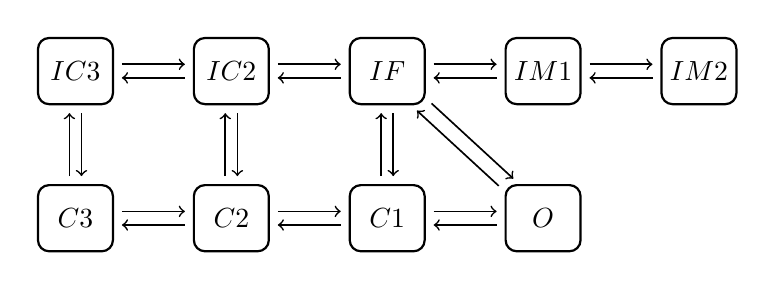
\begin{tikzpicture}[
   font=\sffamily,
   every matrix/.style={ampersand replacement=\&,column sep=1cm,row sep=1cm},
   state/.style={draw,thick,rounded corners,inner sep=.3cm},
   to/.style={->,semithick,shorten >=0.1cm,shorten <=0.1cm},
   Q/.style={->,semithick,sloped,pos=0.700000,shorten >=0.1cm,shorten <=0.1cm},
   every node/.style={auto}]
\matrix{
\node[state] (IC3) {\parbox{10pt}{\centerline{$IC3$}}};\&\node[state] (IC2) {\parbox{10pt}{\centerline{$IC2$}}};\&\node[state] (IF) {\parbox{10pt}{\centerline{$IF$}}};\&\node[state] (IM1) {\parbox{10pt}{\centerline{$IM1$}}};\&\node[state] (IM2) {\parbox{10pt}{\centerline{$IM2$}}};\\
\node[state] (C3) {\parbox{10pt}{\centerline{$C3$}}};\&\node[state] (C2) {\parbox{10pt}{\centerline{$C2$}}};\&\node[state] (C1) {\parbox{10pt}{\centerline{$C1$}}};\&\node[state] (O) {\parbox{10pt}{\centerline{$O$}}};\&\\
};
\draw[to]  (IC3.10) to node {$$} (IC2.170);
\draw[to]  (IC3.280) to node {$$} (C3.80);
\draw[to]  (IC2.190) to node {$$} (IC3.350);
\draw[to]  (IC2.10) to node {$$} (IF.170);
\draw[to]  (IC2.280) to node {$$} (C2.80);
\draw[to]  (IF.190) to node {$$} (IC2.350);
\draw[to]  (IF.10) to node {$$} (IM1.170);
\draw[to]  (IF.280) to node {$$} (C1.80);
\draw[Q]  (IF.325) to node {$$} (O.125);
\draw[to]  (IM1.190) to node {$$} (IF.350);
\draw[to]  (IM1.10) to node {$$} (IM2.170);
\draw[to]  (IM2.190) to node {$$} (IM1.350);
\draw[to]  (C3.100) to node {$$} (IC3.260);
\draw[to]  (C3.10) to node {$$} (C2.170);
\draw[to]  (C2.100) to node {$$} (IC2.260);
\draw[to]  (C2.190) to node {$$} (C3.350);
\draw[to]  (C2.10) to node {$$} (C1.170);
\draw[to]  (C1.100) to node {$$} (IF.260);
\draw[to]  (C1.190) to node {$$} (C2.350);
\draw[to]  (C1.10) to node {$$} (O.170);
\draw[Q]  (O.145) to node {$$} (IF.305);
\draw[to]  (O.190) to node {$$} (C1.350);
\end{tikzpicture}
\end{center}
\caption{The sodium channel model of Clancy et al. \cite{Clancy2002}\label{clancy}; O is the open state, C1, C2 and C3 are the closed states, while the rest of the states represent different kinds of inactivation.}
\end{figure}
%{\it Glenn: forklar hva IM1, IM2 osv betyr i dette skjemaet.}

The popularity of these models stems from the fact that it is possible to adjust the parameters involved to obtain a model that reflects data quite well. However, it should also be mentioned that models can be so complex that it is virtually impossible to uniquely determine all the parameters involved. In these notes, we shall confine ourselves to relatively simple Markov models but the methods we describe can be applied, at least in principle, to Markov models of higher complexity.


\subsection{The master equation}
\label{master_equation}

From the Markov model written on the form (\ref{Markov1}), we can derive an equation
giving the evolution of the probability of the two states, open (O) and closed (C). Let $o=o(t)$ be the
probability that the channel is in the open (O) state at time $t$ and let $c=c(t)$ denote
the probability that the channel is closed (C). We assume that the probabilities $o$ and $c$ are known at time
$t$ and then use the Markov model (\ref{Markov1}) to compute the probabilities at time $t+\Delta t$.
 Here $\Delta t$ is assumed to be so small that the channel changes state at most once during the time step from $t$ to $t+\Delta t$.   Then the scheme (\ref{Markov1}) states that
the open probability at time $t+\Delta t$ is given by
\begin{align}
o(t+\Delta t) &= \text{Prob}\left[  (S(t)=C)  \mbox{\ and\ }  (C\rightarrow O \mbox{\ during\ } \Delta t)  \right] \\
& \ \ \ \ + \text{Prob}\left[  (S(t)=O)  \mbox{\ and not}  (O\rightarrow C \mbox{\ during\ } \Delta t)  \right] \\
&= c(t) \cdot (\Delta t k_{co}) + o(t) \cdot (1 -\Delta t k_{oc})
\end{align}
so
\[
o(t+\Delta t)=o(t)+\Delta t ( k_{co}c(t)-k_{oc}o(t)).
\]
%which expresses the fact that, during the time step from $t$ to $t+\Delta t$, the channel either remain open (first term), it changes from open to close (second term) or it changes from closed to open (last term).
From this equation, we obtain
\[
\frac{o(t+\Delta t)-o(t)}{\Delta t}=k_{co}c(t)-k_{oc}o(t),
\]
and, therefore, by passing to the limit $\Delta t\rightarrow0,$ we get the
differential equation
\begin{equation}
o^{\prime}(t)=k_{co}c(t)-k_{oc}o(t).\label{po}
\end{equation}
Similarly, we find that the probability of being in the closed state evolves
according to
\begin{equation}
c^{\prime}(t)=k_{oc}o(t)-k_{co}c(t).\label{pc}
\end{equation}
Since we are dealing with probabilities, it is reasonable to assume that the
initial conditions add up to one (the channel is either open or closed) and therefore, by adding the equations
above, we find that
\[
o(t)+c(t)=1
\]
for all time. Hence the variable $c$ in (ref{po}) can be
replaced by $1-o$ and the system (ref{po},\ref{pc}) can be
written as a scalar equation of the form
\begin{equation}
o^{\prime}(t)=\left(  k_{co}+k_{oc}\right)  \left(  \frac{k_{co}}
{k_{co}+k_{oc}}-o\left(  t\right)  \right)  .\label{po2}
\end{equation}
Here we see that
\[
o=\frac{k_{co}}{k_{co}+k_{oc}}
\]
is a stable equilibrium solution. Furthermore, if we know that the channel is
closed initially, that is, $o(0)=0,$ we get the solution
\[
o(t)=\frac{k_{co}}{k_{co}+k_{oc}}\left(  1-e^{-\left(  k_{co}+k_{oc}\right)
t}\right)
\]
and we notice that the equilibrium is reached more quickly as the sum of the rates
$k_{co}+k_{oc}$ increases.

\subsection[Three state model]{The master equation of a three-state model}

The development of the master equation for the two-state model above can be
carried out for any Markov model. For instance, if we consider the three-state
Markov model shown in Figure \ref{IOC_me}, we realize that the probabilities of the
open (O), closed (C), and inactivated (I) states are governed by the following system of ordinary
differential equations:
\begin{align}
o^{\prime}  & =k_{io}i+k_{co}c-\left(  k_{oi}+k_{oc}\right)  o, \nonumber \\
c^{\prime}  & =k_{oc}o+k_{ic}i-\left(  k_{co}+k_{ci}\right)  c,\label{me_11}\\
i^{\prime}  & =k_{oi}o+k_{ci}c-\left(  k_{io}+k_{ic}\right)  i, \nonumber
\end{align}
Since
\begin{equation}
i=1-\left(  o+c\right),
\end{equation}
we have the following $2 \times 2$ system:
\begin{align}
o^{\prime}  & =k_{io}+\left(  k_{co}-k_{io}\right)  c-\left(  k_{oi}
+k_{oc}+k_{io}\right)  o,\label{me_20}\\
c^{\prime}  & =k_{ic}+\left(  k_{oc}-k_{ic}\right)  o-\left(  k_{co}
+k_{ci}+k_{ic}\right)  c.\label{me_21}
\end{align}
We will now show, using a numerical computation, that the solution of the
system (\ref{me_20},\ref{me_21}) coincides with the average result of Monte Carlo simulations using
the Markov model shown in Figure \ref{IOC_me} as the number of Monte Carlo runs goes
to infinity.



\begin{figure}[ptb]
\begin{center}
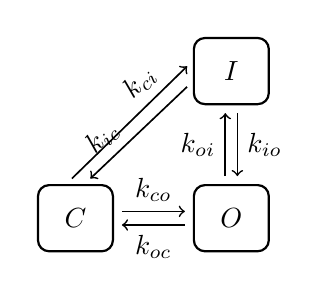
\begin{tikzpicture}[
   font=\sffamily,
   every matrix/.style={ampersand replacement=\&,column sep=1cm,row sep=1cm},
   state/.style={draw,thick,rounded corners,inner sep=.3cm},
   to/.style={->,semithick,shorten >=0.1cm,shorten <=0.1cm},
   Q/.style={->,semithick,sloped,pos=0.700000,shorten >=0.1cm,shorten <=0.1cm},
   every node/.style={auto}]
\matrix{
\&\node[state] (I) {\parbox{10pt}{\centerline{$I$}}};\\
\node[state] (C) {\parbox{10pt}{\centerline{$C$}}};\&\node[state] (O) {\parbox{10pt}{\centerline{$O$}}};\\
};
\draw[to]  (O.100) to node {$k_{oi}$} (I.260);
\draw[to]  (O.190) to node {$k_{oc}$} (C.350);
\draw[to]  (I.280) to node {$k_{io}$} (O.80);
\draw[Q]  (I.195) to node {$k_{ic}$} (C.75);
\draw[to]  (C.10) to node {$k_{co}$} (O.170);
\draw[Q]  (C.105) to node {$k_{ci}$} (I.165);
\end{tikzpicture}
\end{center}
\caption{Markov model including three possible states: open (O), closed (C), and
inactivated (I).}
\label{IOC_me}
\end{figure}




\subsection[Monte Carlo Simulations]{Monte Carlo simulations based on the Markov model}
\label{MCSMM}

Before we compare the two computational schemes, let us briefly describe how
the Monte Carlo simulation can be implemented. We choose a small timestep
$\Delta t$ and we assume that the state at time $t=t_{n}=n\Delta t,$ where $n$
is a non-negative integer, is either O, C, or I. For simplicity, we describe how
the computation proceeds in the case of the channel being in the open (O)
state at time $t=t_{n}$. In order to decide the state at time $t_{n+1}=t_{n}+\Delta t,$ we
divide the unit interval into three non-overlapping parts:  $A_{c}=\left[
0,k_{oc}\Delta t\right)  ,$ $A_{i}=\left[  k_{oc}\Delta t,k_{oc}\Delta
t+k_{oi}\Delta t\right)  ,$ $A_{o}=\left[  k_{oc}\Delta t+k_{oi}\Delta
t,1\right]  .$ Then, at time $t_{n+1}=t_{n}+\Delta t,$ we can update the state
of the channel based on a random number $r_{n}$ in the unit interval drawn from
a uniform distribution. Specifically, if $r_{n}\in A_{o},$ the channel
remains open; if $r_{n}\in A_{c},$ the state of the channel changes from
open to closed; and, finally, if $r_{n}\in A_{i},$ the state of the channel
changes from open to inactivated.

Similar steps are straightforward to
devise for the case of the channel being in the closed or inactivated states
at time $t=t_{n}.$



\subsection[Monte Carlo simulation vs Master Equation]{Comparison of Monte Carlo simulations and solutions of the
master equation}

In Figure \ref{Introduction_L:ode_mc} we compare the probabilities computed by solving the master equation (ref{me_20},\ref{me_21}) (red lines) and by Monte Carlo simulations using the Markov model as described above. In the simulations we have used the initial conditions $o(0)=i(0)=0$
and $c(0)=1$ and the rates used in the computations are given in Table \ref{tab:const3x3}. As the number of Monte Carlo simulations increases, we see that the average approaches the solution of the continuous master equation. In these computations the master equation was solved using the function \GTLV{ODE15s in Matlab}.


\begin{table}  \begin{center}
\begin{tabular}{|r|r|r|r|r|r|} \hline
$k_{oi}$ & $k_{io}$ & $k_{co}$ & $k_{oc}$ & $k_{ic}$ &$k_{ci}$  \\ \hline
0.5  &    0.3 &   0.6   &  0.9  &   0.72  & 0.8 \\ \hline
\end{tabular} \end{center}
\caption{Rates (in 1/ms) of the Markov model given in Figure  \ref{IOC_me} used in the computations presented in Figure \ref{Introduction_L:ode_mc}.}
 \label{tab:const3x3}  \end{table}


%xxGlenn: Lag gjerne 3x3 paneler, der o,c,og i g\aa r fra venstre mot h\o yre og der antall MC \o ker (og dt reduseres) ovenfra og ned. Alle detaljer i caption og i tabellene nevnt over.

FIGURE: [fig/Introduction_L_ode_mc.pdf, width=500 frac=0.8]  Comparison of the solution of the master equation (ref{me_20},\ref{me_21}) (red lines) and the results of Monte Carlo simulations based on the Markov model given in Figure \ref{IOC_me}. The time step used in the Monte-Carlo simulations was $\Delta t$ = 0.01 ms in all the panels and the simulations were run for 10 ms. The number of Monte Carlo simulations increases from 100 (top) to 10,000 (bottom). label{Introduction_L:ode_mc}


\subsection{Equilibrium probabilities}
\label{eq_prob_ioc}

The equilibrium state of the
reaction shown in Figure  \ref{IOC_me} is characterized by the equations
\begin{align}
k_{co}c  &  =k_{oc}o, \nonumber\\
k_{oi}o  &  =k_{io}i, \label{me_eq_20}\\
k_{ic}i  &  =k_{ci}c, \nonumber
\end{align}
where $o,c,$ and $i$ denote the probabilities of the channel being open,
closed, or inactivated, respectively. It follows that
\[
c=\frac{k_{oc}}{k_{co}}o
\]
and
\[
i=\frac{k_{oi}}{k_{io}}o.
\]
By using the fact that $o+c+i=1,$ we obtain
\[
\left(  1+\frac{k_{oc}}{k_{co}}+\frac{k_{oi}}{k_{io}}\right)  o=1
\]
and therefore
\begin{align*}
o  &  =\frac{1}{1+\frac{k_{oc}}{k_{co}}+\frac{k_{oi}}{k_{io}}},\\
c  &  =\frac{\frac{k_{oc}}{k_{co}}}{1+\frac{k_{oc}}{k_{co}}+\frac{k_{oi}
}{k_{io}}},\\
i  &  =\frac{\frac{k_{oi}}{k_{io}}}{1+\frac{k_{oc}}{k_{co}}+\frac{k_{oi}
}{k_{io}}}.
\end{align*}
For the particular rates given in Table \ref{tab:const3x3}, we get the following equilibrium probabilities: $o=0.24,\, c=0.36$, and
$i=0.4$.

\subsection{Detailed balance}

In order to compute the equilibrium solution of (\ref{me_11}) above, we assumed that each of the sub-transitions of the diagram given in Figure \ref{IOC_me} was in equilibrium. More precisely, we assumed that
\[k_{co}c    =k_{oc}o, \, k_{oi}o =k_{io}i,  \text{ and }k_{ic}i =k_{ci}c. \]
These three relations yield
\begin{equation}
k_{co}k_{oi}k_{ic}=k_{ci}k_{io}k_{oc}. \label {db}
\end{equation}
This relation is referred to as the condition of {\it detailed balance}. In these notes, we will always assume that Markov models satisfy this condition. More generally, the product of the rates in a loop (e.g. the I-O-C loop of Figure \ref{IOC_me}) in the clockwise direction equals the product of the rates in the counterclockwise direction. Under this assumption, the equilibrium solution can always be computed by the method indicated above. We will use the same technique many times in these notes.



\section{The master equation and the equilibrium solution}
\label{me_eq}

We have seen that the Markov model written in the form
\begin{equation}
C\underset{k_{co}}{\overset{k_{oc}}{\leftrightarrows}}O \label{Markov1010}
\end{equation}
leads to a master equation of the form
\begin{align}
o^{\prime}(t)=  &  k_{co}c(t)-k_{oc}o(t),\label{po1010}\\
c^{\prime}(t)=  &  k_{oc}o(t)-k_{co}c(t). \label{pc1010}
\end{align}
Since $o+c=1,$ we can reduce the system to the scalar equation,
\[
o^{\prime}(t)=\left(  k_{co}+k_{oc}\right)  \left(  \frac{k_{co}}
{k_{co}+k_{oc}}-o\left(  t\right)  \right)
\]
and we readily see that the equilibrium solution is given by
\[
o=\frac{k_{co}}{k_{co}+k_{oc}}.
\]
Exactly the same steps can be followed for the three-state Markov model
illustrated in Figure \ref{IOC_me}. The associated Markov model reads
\begin{align*}
o^{\prime} &  =k_{io}i+k_{co}c-\left(  k_{oi}+k_{oc}\right)  o\\
c^{\prime} &  =k_{oc}o+k_{ic}i-\left(  k_{co}+k_{ci}\right)  c\\
i^{\prime} &  =k_{oi}o+k_{ci}c-\left(  k_{io}+k_{ic}\right)  i
\end{align*}
and since
\begin{equation}
i=1-\left(  o+c\right)  \label{i4010}
\end{equation}
we arrive at the following $2 \times 2$ system:
\begin{align*}
o^{\prime} &  =k_{io}+\left(  k_{co}-k_{io}\right)  c-\left(  k_{oi}
+k_{oc}+k_{io}\right)  o,\\
c^{\prime} &  =k_{ic}+\left(  k_{oc}-k_{ic}\right)  o-\left(  k_{co}
+k_{ci}+k_{ic}\right)  c.
\end{align*}
The equilibrium solution is now defined by a $2 \times 2$ linear system of equations of
the form
\begin{equation}
Bq=b,\label{i4011}
\end{equation}
where
\[
B=\left(
\begin{array}
[c]{cc}
k_{oi}+k_{oc}+k_{io} & k_{io}-k_{co}\\
k_{ic}-k_{oc} & k_{co}+k_{ci}+k_{ic}
\end{array}
\right)  ,\;q=\left(
\begin{array}
[c]{c}
o\\
c
\end{array}
\right)  \text{, and }b=\left(
\begin{array}
[c]{c}
k_{io}\\
k_{ic}
\end{array}
\right)  .\;
\]
By solving this linear system and using (ref{i4010}), we
find (as above) that

\[
o=K^{-1},\;c=\;\frac{k_{oc}}{k_{co}}K^{-1},\;i=\frac{k_{oi}}{k_{io}}K^{-1},
\]
where
\[
K=1+\frac{k_{oc}}{k_{co}}+\frac{k_{oi}}{k_{io}}.
\]

\subsection[Linear algebra]{Linear algebra approach to finding the equilibrium solution}

Calculations to find the equilibrium solution will be done repeatedly in these notes. We
will always use the special structure of the Markov model to derive the
equilibrium solution, but it also worth noting that this can be done by
solving a linear system. The master equation associated with a Markov model of the
form  (ref{Markov1010}) or of the form given in
Figure \ref{clancy} can always be written in the form
\[
p^{\prime}=Ap,
\]
where $p$ is a vector containing the probabilities of occupying the different
states of the Markov model. Since the sum of the probabilities adds up to one,
the number of unknowns can be reduced by one and the system takes the form
\[
q^{\prime}=b-Bq.
\]
Therefore, the equilibrium solution can be found by solving the linear system
(ref{i4011})

Instead of reducing the number of unknowns, we can also address the problem more directly by computing the eigenvector
associated the eigenvalue $\lambda = 0$. For instance, using Matlab  we can put $z=\rm{null}(A)$ and then define
\[p=\frac{z}{\sum_i z_i}\]
 where
$z_i$ denote the components of the vector $z$.


\section[Stochastic simulations and PDFs]{Stochastic simulations and probability density functions}

Given the Markov model, defining a stochastic differential equation describing changes of the transmembrane potential due to the opening and closing of the channel is quite straightforward. Additionally, based on the stochastic differential equation, we will derive deterministic differential equations describing the probability density functions of the states involved in the Markov model. We thus have two ways to analyze models of ion channels: We can either run numerous Monte Carlo simulations using the stochastic differential equation or solve the deterministic differential equations defining the probability density functions. Both these methods will be used throughout the notes. Although one method is the average of the other, we will see that both provide distinct insights useful to understanding the mechanisms under consideration.


\section{Markov models of calcium release}
The contraction of the heart is a collective and very well-coordinated effort achieved in a collaboration involving billions of cells. For each of these cells, the contraction depends on the release of a massive amount of calcium from internal storage. The release takes place in many thousands of release units within each cell and the state of the release process is believed to be adequately modeled using Markov models.

We will study this release in several steps and we start by assuming that the only varying concentration is in the dyad and that the reaction rates of the Markov model vary only with this single concentration. This case will be studied in great detail and we will explain how drugs can be theoretically constructed to repair mutations affecting the release mechanism. The analysis is based on a scalar stochastic differential equation representing the concentration of calcium in the dyad. The properties of this model will be analyzed using Monte Carlo simulations. Furthermore, we will derive a system of deterministic partial differential equations describing the probability density function of the states of the Markov model.

It is more common to divide the calcium concentration into two values---not only one---which leads to  $2\times2$ stochastic differential equations to be analyzed. This model will also be analyzed using Monte Carlo simulations and by a 2D deterministic system of partial differential equations representing the probability density functions of the states of the Markov model.

Next, we shall couple the calcium concentration to the voltage-gated release of calcium through so-called L-type calcium channels. This model will allow us to study optimal drugs, combining the effect on calcium release and L-type channels. The balance of these mechanisms rules the calcium-induced calcium release that is at the crux of cardiac contraction. The calcium-induced calcium release model is stated in terms of a $2\times 2$ model of stochastic equations where the transmembrane potential $V$ is included as a parameter in the model. The associated model for the probability density functions is given by a 2D system of partial differential equations where the transmembrane potential is again included as a parameter.

 \section{Markov models of ion channels}

After analysis of the calcium release we move on to study voltage-gated  ion channels. We will immediately see that in mathematical terms the problem is very similar to the calcium release problem. For the ion channel case, however, the stochastic equation is one-dimensional and so is the associated deterministic partial differential equation. The basic Markov model is still based on the open and closed states, but we will also see that an inactivated state plays a central role. Optimal theoretical drugs will be derived and we will observe that they work nicely.

\section{Mutations described by Markov models}

A trademark of mutations affecting ion channels and calcium release mechanisms is that they change the open probability and possibly also the mean open time and other characteristics of the channels involved. We will show below that the equilibrium open probability of the channel described by the Markov model of the form (\ref{Markov1}) is given by
\[ o=\frac{k_{co}}{k_{co}+k_{oc}} \]
and the mean open time is given by
\[ \tau_o=\frac{1}{k_{oc}}. \]
The concept of mean open time will be discussed in Chapter \ref{mot_chapter} and the formula $\tau_o=1/k_{oc}$ will be derived in that chapter.
 Given these formulas, it is straightforward to see that the effect of mutations affecting the open probability or the mean open time can be modeled by changing the parameters of the Markov model. In these notes we shall focus on rather simple changes
 in the model but, again, the techniques can be generalized to more intricate cases.

  Two examples of the effect of mutations are given in Figures
 \ref{Introduction_L:Loaiza_crop}  and \ref{Introduction_L:chandra}. Figure
 \ref{Introduction_L:Loaiza_crop}  shows recordings of the open and closed states for the wild type and the
  V2475F mutation of the ryanodine receptor (RyR).
  The graphs in Figure \ref{Introduction_L:chandra} show similar results for the voltage-gated sodium channel when the wild type recordings are compared with recordings from a mutant ($\Delta$KPQ) channel.


FIGURE: [fig/Introduction_L_Loaiza_crop.png, width=500 frac=0.8] Single-channel recordings of wild type (black) and mutant (red) cardiac RyR channels. The open probability and the mean open time are significantly increased for the mutant (V2475F) case. The graphs are from Figure 3 of Loaiza et al. \cite{loaiza2013}. label{Introduction_L:Loaiza_crop}

FIGURE: [fig/Introduction_L_chandra.png, width=500 frac=0.8] Sodium current recordings taken from Figure 4 of Chandra et al. \cite{Chandra1998}: A represents the wild type and B represents
the $\Delta$KPQ mutant. The recordings are based on 200-ms depolarizing pulses from -100 mV to -40 mV.  label{Introduction_L:chandra}


\section{The problem and steps toward solutions}

Assume that experimental data on wild type cells can be used to identify the parameters of a Markov model faithfully describing the stochastic properties of the wild type channel and that experimental data on mutant cells can be used to establish a Markov model of similar structure representing the stochastic properties of the mutant channel. Furthermore, we assume that the Markov model of the mutant can be extended to account for the effect of a theoretical drug. {\it The problem is then to compute the reaction rates of the drug such that, after the drug is applied, the mutant channel behaves as similarly to the wild type channel as possible. } The essence of these notes is to show how to solve this problem mathematically; we show how to compute an optimal theoretical drug. To clarify what we mean by an optimal theoretical drug, we will give a few examples that will be discussed later and then we will briefly discuss the concept of a theoretical drug  more generally.

 \subsection{Markov models for drugs: Open state and closed state blockers}
 By using the notation of chemical reactions introduced above, we can explain the problem in a bit more detail. The reaction scheme for an open state blocker can be illustrated as follows:
\begin{equation}
C\underset{ k_{co}}{\overset{k_{oc}}{\leftrightarrows}}O\underset{k_{ob}
}{\overset{k_{bo}}{\leftrightarrows}}B. \label{open_block}
\end{equation}
For theoretical purposes, this drug is well defined, provided that we know the values of the parameters $k_{ob}$ and $k_{bo}$. We will often assume that these parameters are constants. As mentioned above, one example of a problem we want to overcome
is mutations leading to an increased open probability; so either the release mechanism is too prone to releasing calcium from internal storage or the ion channels are too prone to allowing  current to flow through the cell membrane.

Since the problem involves too high of an open probability, it seems reasonable to try to fix the open probability by extending the reaction scheme and directly affecting this state, as illustrated in the reaction scheme above. By allowing the probability to be moved from $O$ to $B$, the open probability will be reduced and thus the goal will be achieved. This reasoning seems impeccable and it seems much less intuitive to use a closed state drug of the form
\begin{equation}
B\underset{k_{bc}}{\overset{k_{cb}}{\leftrightarrows}}C\underset{
k_{co}}{\overset{k_{oc}}{\leftrightarrows}}O. \label{closed_block}
\end{equation}
We will see, however, that both open and closed state blockers may be optimal, depending on the nature of the mutation.

\subsection{Closed to open mutations (CO-mutations)}
\label{com}
We have seen that for a Markov model written in the form
\begin{equation}
C\underset{ k_{co}}{\overset{k_{oc}}{\leftrightarrows}}O,
\end{equation}
 the equilibrium open probability is given by
\[ o=\frac{k_{co}}{k_{co}+k_{oc}}=\frac{1}{1+\frac{k_{oc}}{k_{co}}} \]
and the mean open time is given by
\[ \tau_o=\frac{1}{k_{oc}}. \]
A mutation leading to an increased open probability can be represented by a Markov model written in the form
\begin{equation}
C\underset{ \mu k_{co}}{\overset{k_{oc}}{\leftrightarrows}}O,
\end{equation}
where $\mu \ge 1$ will be referred to as the {\it mutation severity index} and we always use the convention that $\mu=1$ refers to the wild type case. At this point, it is useful to recall the interpretation of a scheme of this form. In particular, it is useful to note that the probability of going from the closed state (C) to the open state (O) during a time step $\Delta t$ is now given
by $\mu \Delta t k_{co}$, compared to $\Delta t k_{co}$ for the wild type channel. It is pretty clear that increasing the mutation severity index will increase the probability of being in the open state and this is also reflected by the equilibrium open probability given by
\[o_\mu=\frac{1}{1+\frac{k_{oc}}{\mu k_{co}}}, \]
which clearly increases as a function of the mutation severity index $\mu$.
It is also interesting to observe that, for this mutation, the mean open time is unchanged. We will refer to a mutation of this form as a CO-mutation and we will show repeatedly that, for CO-mutations, closed state blockers are theoretically optimal.

\subsection{Open to closed mutations (OC-mutations)}
Another way to introduce a mutation that increases the open probability is to decrease the rate from open to closed. This can be written as follows:
\begin{equation}
C\underset{ k_{co}}{\overset{k_{oc}/\mu}{\leftrightarrows}}O,
\end{equation}
where, again, $\mu \ge 1$ is the mutation severity index and $\mu=1$ represents the wild type. The probability of leaving the open state is now reduced and this will lead to an increased open probability.
In particular, the equilibrium open probability is again given by
\[ o_\mu=\frac{1}{1+\frac{k_{oc}}{\mu k_{co}}}, \]
as above, but now the mean open time changes; it is given by
\[ \tau_o=\frac{\mu}{k_{oc}}\]
and thus increases with the mutation severity index.

We will refer to a mutation of this form as an OC-mutation and we will show that, for such mutations, open state blockers are theoretically optimal.

\section{Theoretical drugs}
\label{theoreticaldrugs}

The concept of a theoretical drug is essential in these notes. Basically, we will {\em  refer to a theoretical drug\footnote{We also use the terms \textit{mathematical drug, numerical drug}, and so forth interchangeably with \textit{theoretical drug}} as a purely mathematical construction} that may or may not have a viable pharmaceutical counterpart. A mental image of how the drug may work is given in Figure \ref{Introduction_L:drg_starmer}; the figure is taken from Starmer \cite{Starmer2002}. With no drug involved, the channel can take on two conformational states: the open state (O), when ions can flow freely through the channel, and the closed state (C), when there is no flow of ions through the channel. An open blocker can change the open state such that there is no flow through the channel. The reaction scheme of the situation described in the figure is given by
\begin{equation}
C\underset{ k_{co}}{\overset{k_{oc}}{\leftrightarrows}}O\underset{k_{ob}
}{\overset{k_{bo}}{\leftrightarrows}}B. \label{closed_block201}
\end{equation} where we again note that the properties of the theoretical drug are solely given by the values of the rates $k_{ob}$ and $k_{bo}$.

This way of describing the effect of a drug has been used for many years, see e.g. Hille \cite{Hille1977} or Hondeghem and Katzung \cite{Hondeghem1977}. Our use of this notation is clearly motivated by the paper of Clancy et al. \cite{Clancy2007}. In these papers, an existing drug is characterized using a scheme of the form (\ref{closed_block201}). That is, data obtained from experiments using a particular drug are used to characterize the rates $k_{bo}$ and $k_{ob}$ referred to, respectively, as the on and off rates of the drug. As mentioned above, we often view the rates as free parameters that can be optimized in order to create the best possible theoretical drug in the sense that the channel should work as much like the healthy case as possible. This way of describing a theoretically optimal drug was introduced in \cite{Tveito2011c} and clearly motivated by the drug vector approach discussed in   \cite{Tveito2009}.

FIGURE: [fig/Introduction_L_drg_starmer.png, width=500 frac=0.8] Illustration of a blocker associated with the open state. In the leftmost case the channel is closed and no ions can pass through it. In the center case, the channel is open and ions may flow freely. In the rightmost case the channel is blocked by the drug and no ions can pass through it. The figure is taken from Starmer \cite{Starmer2002}. label{Introduction_L:drg_starmer}

\section{Results}
Many of the models, methods, and results described in these notes are well known in the literature. All the Markov models are taken from the literature and so are the stochastic differential equations and the models describing the probability density approach. Compared to earlier published models, we will often derive simplified models, but the ideas behind them are basically the same as those used by many authors. Concerning the modeling of mutations, we aim to consistently model the effect of mutations as simply as possible and preferably only by changing a single parameter: the mutation severity index.

The novel part of these notes is that we attempt to systematically describe how to compute characterizations of drugs that are optimal in a specific sense and we do so for a number of applications. We almost exclusively address so-called gain-of-function mutations. For such mutations, the open probability of the channel or receptor is too large, which can lead to severe difficulties for the cell and, ultimately, for large collections of such cells.

%We begin by studying such mutations in cases where the mean open time is unaltered. In such cases, we give several examples indicating that closed blockers are much better suited for repairing the effect of the mutation than open blockers. If, on the other hand, both the open probability and the mean open time is affected, open state blockers are to be preferred. In a similar manner we discuss how to deal with mutations that impair the inactivation of ion channels.

\section{Other possible applications}

The focus in this text will be on how to compute characterizations of optimal theoretical drugs defined in terms of parameters describing the associated Markov model. The methods can, however, also be used to compare existing drugs. If Markov models are developed for two drugs, the associated probability density functions can be computed and thus a comparison of the quality of the two drugs can be computed. This approach will rely heavily on accurate representations of the function of a drug in terms of a Markov model, which is a problem beyond the scope of the present notes.


\section{Disclaimer}
These notes are written to explain in some detail how we can compute characterizations of theoretical drugs in terms of Markov models. However, we specifically avoid discussing whether it is possible to realize a certain drug given the characterization in terms of a Markov model, simply because we do not know and have been unable to find any reasonable answer to this in the literature.  The applicability of our results therefore remains uncertain.


\section{Notes}
\begin{enumerate}
\item Several excellent introductions to Markov models of the stochastic behavior of receptors and ion channels are available (e.g., \cite{KeenerSneyd, Smith2002, Jacobs2010, Santillan2014}). In particular we recommend the recently published book by Bressloff \cite{Bressloff2014} (see also \cite{Bressloff2014w}). Bressloff \cite{Bressloff2014} provides a broad introduction to stochastic processes in cells and covers most of the models covered in the present text and much more. It is an excellent text that will become a standard reference in the field.
\item A comprehensive mathematical analysis of the stochastic properties of single ion channels using Markov models was initiated by Colquhoun and Hawkes (e.g., \cite{ Colquhoun1977,Colquhoun1981,Colquhoun1982}).
\item Insight into the electrophysiology of excitable cells was fundamentally enhanced by the development of the patch clamp technique of Sakmann and Neher (see, e.g., \cite{Sakmann1984,Sakmann1995}). The authors received the Nobel Prize in Physiology or Medicine in 1991 for their work on single ion channels. The patch clamp technique is used to generate measurements of the form illustrated in
Figure \ref{Introduction:na_cropped}. These data are used to determine the Markov model and are therefore of fundamental importance. As mentioned below, however, the problem of finding the Markov model based on experimental data is still an active research problem.
\item The models studied in these notes address the flow of ions through various types of channels. An excellent introduction to ion channels is given in the book by Hille \cite{Hille2001}.
\item Our discussion is focused on mechanisms of the heart but, at the level of single channels, these mechanisms are similar to channel-based mechanisms of the brain or, more specifically, the mechanisms of neurons. There are several excellent introductions to neuroscience
(e.g., \cite{Ermentrout2010,Sterratt2011,Dayan2001,Izhikevich2007}).
\item
Given the Markov model, we have seen that it is pretty straightforward to compute what state the channel is in as a stochastic function of time. We have also seen that we can solve the master equation and find the average behavior of the channel when the rates are independent of the surroundings. Furthermore, we will show how to compute probability density functions for each state when the rates depend on the transmembrane potential. Such simulations are forward problems: Given the model,  compute the solution. The inverse problem in this setting is quite a bit harder; the problem is to compute the rates (i.e., the values of $k_{oc},\,  k_{co}$ etc.) of the Markov model in order for the stochastic behavior of the model to match the measurements of the channel. The analysis of the inverse problem was started by Colquhoun and Hawkes \cite{Colquhoun1977}, beginning in 1977, and their findings are summarized by Sakmann and Neher \cite{Sakmann1995} (see also
\cite{Colquhoun1996}). More recently the problem has been addressed in a series of papers by Sachs and his co-authors; see \cite{Qin1996,Qin2000,Nicolai2013}. Their methods are available in the open-source QuB software package. Furthermore, Markov chain Monte Carlo (MCMC) has been used in a series of papers by Siekmann, Sneyd and his co-authors \cite{Gin2009,Siekmann2011,Siekmann2012, Siekmann2014}. Interestingly, their analysis shows that certain Markov models cannot be identified using standard data. The MCMC method was used for inversion of single ion channel data more than 15 years ago by Ball et al \cite{Ball1999}, and Rosales and co-authors, see \cite{Rosales2001,Rosales2004}.
\item For whole cell data, the problem of identifying the parameters of Markov models is carefully studied by Fink and Noble \cite{Fink2009}.
\item The terms {\it CO-mutation}, {\it OC-mutation}, and {\it mutation severity index} are not standard and introduced here for convenience.
\item A thorough discussion of the principle of detailed balance can be found in the paper by  Colquhoun et al. \cite{Colquhoun2004}. The validity of the principle for given data can be tested as shown by Song and Magleby \cite{Song1994} and Ullah et al. \cite{Ullah2012} (suppl. material).
There are examples of Markov models that do not satisfy the principle of detailed balance (see, e.g., \cite{Bressloff2014}, p. 208).
\item The numerical method for handling the Markov model described on page \pageref{MCSMM} is not particularly efficient. For the case of constant rates in the Markov model, considerable acceleration can be achieved by using the method of Gillespie \cite{Gillespie1977}. The Gillespie method is particularly useful for simulations involving many channels (see, e.g., \cite{Smith2002}).
\item For comprehensive introductions to modeling the cardiac action potential, we refer to the recent overview by Rudy \cite{Rudy2012} and to Rudy and Silva \cite{Rudy2006}.  For the action potential shown in Figure \ref{Introduction_L:grandi}, we used the model of Grandi et al. \cite{Grandi2010B}. An alternative is the model of O'Hara et al. \cite{Ohara2011} and a huge collection of models is available at the CellML project (CellML.org).
\item The dynamics of cardiac electrophysiology are introduced in numerous papers and books; a recent comprehensive review is provided by Qu et al. \cite{Qu2014}.  The book by Katz \cite{Katz2010}
is a standard reference in cardiac physiology and the book by Glass et al. \cite{Glass2012} is a standard reference in the modeling of the heart. Numerical methods for the simulation of cardiac electrophysiology are presented by Sundnes et al. \cite{Sundnes2007} (see also \cite{Pullan2005, Franzone2014}).



\end{enumerate}











\chapter{One-dimensional calcium release}
\label{Ca_release_1D}

The contraction of a single cardiac cell is initiated by an increase in the transmembrane potential leading to opening of the so-called L-type calcium channels (LCCs). When these channels are open, calcium flows into a rather small space called the dyadic cleft (often simply referred to as the dyad), leading to a locally increased concentration of Ca$^{2+}$ ions. This increased concentration leads to  the opening of the ryanodine receptors (RyRs), which control the flow of calcium from the internal stores referred to as the sarcoplasmic reticulum (SR). This process is referred to as the calcium-induced calcium release (CICR) and is of vital importance in the functioning of the heart. A schematic description of the process is given in Figure \ref{cicr_1D}. 

%The figure illustrates the essential elements of CICR. Increased transmembrane potential leads to opening of L-type calcium channels (LCCs in the figure) and then Ca$^{2+}$ ions flows into the dyad due to a strong concentration gradient. In the dyad, RyRs are calcium sensitive and increases concentration in the dyad leads to opening of the RyRs and then calcium ions flow out of SR (union of JSR and NSR in the figure) and into the dyad. 

This CICR process is one of the focal points of interest in these notes. We shall develop a model coupling the effects alluded to in Figure \ref{cicr_1D}. However, in this first chapter we shall simplify the process quite a bit by assuming that we just have three spaces: the SR, the dyad, and the cytosol (see Figure \ref{geom1D}). This simplification means that we assume that there is very fast diffusion between the network SR (NSR) domain and the junctional SR (JSR) domain such that the associated concentrations are identical. 
Furthermore, we ignore the L-type channels and assume that the concentrations in both the SR and the cytosol are constant. This leads to a one-dimensional model, in the sense that only the concentration of the dyad changes. The model is useful because it helps illustrate the tools we need in our analysis of the full CICR process and illustrates the properties of optimal drugs that will be more or less inherited in more complex models.  

Our aim is therefore to understand in some detail what is going on in the process illustrated in  Figure \ref{cicr_1D}. However, this figure is in itself a huge simplification of the complex CICR process. The cell consists of 10,000 to 20,000 dyads, each dyad having \GTLV[20]{up} to 100 RyRs, and human ventricles consist of billions of cells. Our aim is to focus entirely on a very small but essential element in the CICR mechanism.

\begin{figure}
\centering\resizebox{0.9\linewidth}{!}{\winslow{2.5}{2}{8.5}{6}}
\caption{This figure illustrates the components involved in the CICR: the T-tubule, the dyad, the SR represented by the JSR and NSR, and the cytosol.
%(the light blue area except for the area occupied by the dyad).
Calcium ions can enter the dyad from the T-tubule through LCCs and from the SR through the RyRs. The figure is taken from Winslow et al. \cite{winslow2006}. In this chapter, we concentrate on the dynamics in the box surrounded by a thin red line. Thus we assume that the concentration of the JSR and NSR are identical and constant and we ignore the LCCs. We also assume that all the RyRs are in the same state and therefore can be treated as one channel (see also Notes at page \pageref{notes_Ca_1D}).
\label{cicr_1D}}
\end{figure}

We model the release of Ca$^{2+}$ ions from the SR to the dyad by formulating a stochastic differential equation governing the concentration of Ca$^{2+}$ ions in the dyad. The model will be studied both numerically and analytically and we show how the solution's properties depend on the parameters defining the model. Next, we will derive a deterministic partial differential equation (PDE) giving the probability density function of the states of the Markov model. Although the transition from a stochastic model to a deterministic model for the probability density functions is classical by now, we will spend some time deriving the equations in detail because the transition from stochastic to deterministic is such a wonderful piece of insight. Furthermore, we will provide detailed comparisons of Monte Carlo simulations based on the stochastic model and the probability density functions.
In subsequent chapters, we will develop the model further by using two small spaces, the dyad and the JSR (see Figure \ref{cicr_1D}),  allowing for different concentrations of Ca$^{2+}$ ions. This leads to a two-dimensional (2D) problem. 

Finally, we will take the LCCs into account. This leads to a 2D problem depending on one parameter: the transmembrane potential.

In these notes, we will use the concept of dimension in two different, but related,  ways. In the first version of the stochastic model of CICR, we will model only the concentration of Ca$^{2+}$ in the dyad and we will refer to the model as one dimensional (1D). When a deterministic model governing the probability density function of the states of the Markov model is derived, that model is also 1D in the sense that it depends on one spatial variable; the concentration of Ca$^{2+}$. Next we move to two concentrations (in the dyad and the JSR), leading to a 2D stochastic model in the sense that it is a $2\times 2$ system of stochastic ordinary differential equations. The associated model governing the deterministic probability density functions is also 2D in the sense that the model depends on two spatial variables: the concentration of Ca$^{2+}$ in the dyad and in the JSR. So the general rule is that the number of different concentrations allowed in the system of stochastic ordinary differential equations carries over to the spatial dimension of the deterministic system of PDEs governing the probability density functions of the states involved in the Markov model. Furthermore, the number of states in the Markov model decides the number of equations in the deterministic system of PDEs. 


\section{Stochastic model of calcium release}
\label{stoch}

Suppose that the cytosolic Ca$^{2+}$  concentration is given by $c_{0}$ and the SR
concentration is given by $c_{1}$; we assume both to be constant and that
$c_{1}\gg c_{0}$. We want to model the concentration $\bar{x}=\bar{x}(t)$ in the dyad located
between the cytosol and the SR (see Figure \ref{geom1D}). Throughout these notes, we will use a bar to indicate stochastic variables.

\begin{figure}
[ptb]
\begin{center}
\begin{tabular}{c!{\vrule width 1pt}c!{\vrule width 1pt}c} 
\noalign{\hrule height 1pt}
&& \\
Cytosol, $c_0$ & Dyad, $\bar{x}(t)$ & SR, $c_1$ \ \ \ \ \  \\
&& \\ \noalign{\hrule height 1pt}
\end{tabular}
\caption{Illustration of the model studied in the present chapter: The Ca$^{2+}$ concentration is high in the SR and low in the cytosol. Release from the SR is governed by a Markov model and the
concentration can be diffused from the dyad to the cytosol.}
\label{geom1D}
\end{center}
\end{figure}
%EndExpansion

We assume that there is stochastic release from the SR to the dyad, and diffusion from the dyad to the cytosol. Let $v_{r}$ denote the
speed of release (when the channel is open) and let $v_{d}$ be the speed of diffusion; both are non-negative. Then a stochastic
model of the concentration $\bar{x}=\bar{x}(t)$ in the dyad is given by
\begin{equation}
\bar{x}^{\prime}(t)=\bar{\gamma}(t)v_{r}(c_{1}-\bar{x})+v_{d}(c_{0}-\bar{x}), \label{ode1}
\end{equation}
where the function $\bar{\gamma}=\bar{\gamma}(t)$ takes on the value zero (closed) or one
(open), and the dynamics of the function are governed by a Markov model of the
form
\begin{equation}
C\underset{k_{co}}{\overset{k_{oc}}{\leftrightarrows}}O, \label{Markov}
\end{equation}
with $k_{oc}$ and $k_{co}$ as reaction rates that may depend on the concentration.
Markov models were introduced on page \pageref{markovintro} but let us recall that the 
reaction rates $k_{oc}$ and $k_{co}$ basically indicate the tendency of a channel to change state. So, if 
the channel is open, the probability that the channel changes from open to closed in a very short time interval
$\Delta t$ is given by $\Delta t k_{oc}$ and, similarly, if the channel is closed,
 $\Delta t k_{co}$ is the probability that it becomes open in the time interval $\Delta t$. 
 This means that the higher the rate $k_{co}$,  the more likely it is that the channels are open. This property will be used repeatedly in what follows. 

\subsection{Bounds of the concentration}

Suppose that at time $t=t_{0},$ the channel is closed ($\gamma=0)$, that the
concentration is given by $x(t_0)=x_{0},$ and that the channel remains closed for
$t\leqslant t_{0}+\Delta t.$ Then, in the interval $t_{0}\leqslant t\leqslant
t_{0}+\Delta t,$ the dynamics are given by the deterministic equation\footnote{Note that when we consider the case of a given value
$\gamma$, the model becomes deterministic and we remove the overbar that
indicates a variable is stochastic.}
\[
x^{\prime}(t)=v_{d}(c_{0}-x)
\]
and thus
\[
x(t)=c_{0}+e^{v_{d}(t_{0}-t)}\left(  x_{0}-c_{0}\right)
\]
in this time interval.  Therefore, for a closed channel, the concentration $x(t)$ of the
dyad approaches $c_{0}$ (the cytosolic concentration) at an exponential
rate. The decay is faster for larger values of the diffusion
velocity $v_{d.}$ By consulting Figure \ref{geom1D} we see that this is quite
reasonable; if we close the release from the SR, the concentration of the dyad will gradually approach
the concentration of the cytosol.

Next, we consider the case of an open channel,
\begin{equation}
x^{\prime}(t)=v_{r}(c_{1}-x)+v_{d}(c_{0}-x), \label{open600}
\end{equation}
and again we assume that $x(t_0)=x_0.$
We can rewrite this in the form
\[
x^{\prime}(t)=(v_{r}+v_{d})\left(c_{+}-x\right),
\]
where
\[
c_{+}=\frac{v_{r}c_{1}+v_{d}c_{0}}{v_{r}+v_{d}},
\]
and find that the solution is given by
\[
x(t)=c_{+}+e^{\left(  v_{r}+v_{d}\right)
(t_{0}-t)}\left(  x_{0}-c_{+}\right).
\]
Therefore, when the channel is open, we observe that the concentration $x(t)$ of the dyad approaches $c_{+}$
at an exponential rate. Furthermore, we note that the rate increases with $v_{r}+v_{d}$.
Note also that
\begin{equation}
c_{+}  =c_{1}+\frac{v_{d}\left(  c_{0}-c_{1}\right)  }{v_{r}+v_{d}}<c_{1}.
\end{equation}
So, to summarize, when the channel is open, the concentration approaches  $c_+<c_1$ and when it is closed, the concentration approaches $c_0$. 

For a given state of the channel (open or closed), the concentration profile is monotone and therefore there is no way the solution
can become less than $c_0$ or larger than $c_+$. We therefore have
\begin{equation}
c_{0}\leqslant \bar{x}(t)\leqslant c_{+} \label{invariant}
\end{equation}
for all time, provided that this bound holds initially. 

Note that since $c_{1}\gg c_{0},$ we have
\[
c_{+}\approx\frac{v_{r}}{v_{r}+v_{d}}c_{1}
\]
and therefore $c_{+}$ approaches $c_{1}$ if 
\[\frac{v_{d}}{v_{r}}
\longrightarrow 0.\]
 Suppose, for instance, that we keep $v_{r}$ fixed and we let $ v_{d}$ approach zero. Then 
 $c_{+}$ approaches $c_{1}$, which is reasonable since calcium will be poured into the dyad, but the connection to the cytosol is almost closed and thus the 
dyadic concentration will increase until it reaches an equilibrium with the SR concentration.

\subsection{An invariant region for the solution}

The invariant region (\ref{invariant}) deserves a comment, since it will become quite useful later. Suppose that the initial concentration of the dyad is somewhere in the interval defined by $c_0$ and $c_+$. Then, we have seen that if the channel is either closed or open, the solution remains in this interval as long as the channel does not change state. When the channel changes state, say, at time $t=\Delta t$, we have a new initial condition in the interval $c_0$ and $c_+$ and we can solve the equation deterministically once more and the solution will remain in the interval. The process can be repeated over and over and the solution will always remain in the interval $c_0$ and $c_+$. This property is useful, because it directly implies that the probability of being outside this interval is zero, which is what we need when we want to define boundary conditions for the model defining probability density functions. 

\subsection{A numerical scheme}
\label{numscheme}

To perform stochastic simulations, we discretize the equation
\begin{equation}
\bar{x}^{\prime}(t)=\bar{\gamma}(t)v_{r}(c_{1}-\bar{x})+v_{d}(c_{0}-\bar{x}) \label{sde1D}
\end{equation}
to obtain the explicit scheme
\begin{equation}
x_{n+1}=x_{n}+\Delta t\left( \gamma_{n}v_{r}(c_{1}-x_{n})+v_{d}(c_{0}
-x_{n})\right) \label{sde1D_scheme}
\end{equation}
where $\gamma_{n}$ takes on the value zero (closed) or one (open). The value of $\gamma_{n}$ is computed as follows: Let $\sigma_n$ be a random number in the unit interval. Assume that $\gamma_{n-1}=0$. Then, if $k_{co}\Delta t >\sigma_n$, we set 
$\gamma_{n}=1$, but if this condition does not hold, we set $\gamma_{n}=0$. Similarly, assume that $\gamma_{n-1}=1$. Then, if $k_{oc}\Delta t >\sigma_n$, we set 
$\gamma_{n}=0$, but if this condition does not hold, we set $\gamma_{n}=1$.

\subsection{An invariant region for the numerical solution}
We want to ensure that the numerical scheme provides solutions mimicking the properties of the analytical solutions. Therefore, we want to confirm that the invariant region for model (\ref{sde1D}) also holds for the numerical solutions. For this to hold, we have to assume that the time step is restricted as follows:
\begin{equation}
\Delta t<\frac{1}{v_{r}+v_{d}}. \label{time_step_sode}
\end{equation}
To derive the invariant region, we define
\[
F(x)=x+\Delta t\left(  \gamma_{n}v_{r}(c_{1}-x)+v_{d}(c_{0}-x)\right)
\]
and note that
\[
F^{\prime}(x)=1-\Delta t\left(  \gamma_{n}v_{r}+v_{d}\right)  \geqslant
1-\Delta t\left(  v_{r}+v_{d}\right)  >0.
\]
If we assume that $c_{0}\leqslant x_{n}\leqslant c_{+}$, we obtain
\[
x_{n+1}=F(x_{n})\geqslant F(c_{0})=c_{0}+\Delta t\left(  \gamma_{n}v_{r}
(c_{1}-c_{0})\right)  \geqslant c_{0}
\]
and
\begin{align*}
x_{n+1}  &  =F(x_{n})\\
&\leqslant F(c_{+})\\
&  =c_{+}+\Delta t\left(  \gamma_{n}v_{r}(c_{1}-c_{+})+v_{d}(c_{0}
-c_{+})\right) \\
&  \leqslant c_{+}+\Delta t\left(  v_{r}(c_{1}-c_{+})+v_{d}(c_{0}
-c_{+})\right) \\
&  =c_{+},
\end{align*}
where we have used the fact that
\[ c_{+}=\frac{v_{r}c_{1}+v_{d}c_{0}}{v_{r}+v_{d}}.\]
Therefore, by induction, we have $c_{0}\leqslant x_{n}\leqslant c_{+}$ for all time.


\subsection{Stochastic simulations}

\graytable{l}{
{|c|c|} \hline
$v_d $ & 1 $\rm{ms^{-1}}$\\ \hline
$v_r $ & 0.1 $\rm{ms^{-1}}$\\ \hline
$c_0 $ & 0.1 $\rm{\mu M}$\\ \hline
$c_1 $ & 1000 $\rm{\mu M}$ \\ \hline
$k_{co}(x) $ & $0.1x$ $\rm{ms^{-1}\, \mu M^{-1}} $ \\ \hline
$k_{oc} $ & 1 $\rm{ms^{-1}}$ \\ \hline
}{Parameter values for model (\ref{sde1D}) used in the computations
presented in Figures \ref{1D:mc_ca} and \ref{1D:mc_state}. \label{tab:1Dsode}}

We use the scheme (\ref{sde1D_scheme}) to compute the concentration governed by the model  (\ref{sde1D}),
using the parameters given in Table \ref{tab:1Dsode}.
%$v_d =1\rm{ms^{-1}}$,  $c_0=0.1 \rm{\mu M}$, $v_r=0.1\rm{ms^{-1}}$, $c_1=1000\rm{\mu M}$, 
%$k_{oc}=1 \rm{ms^{-1}}$, and $k_{co}(x)=0.1x\rm{ms^{-1}\, \mu M^{-1}}  $.
The numerical results are given in Figure 
\ref{1D:mc_ca} for time running from $0$ ms to $100$ ms. In Figure  \ref{1D:mc_state}, we show the same solution but focus on the time interval from $20$ ms to $30$ ms. The lower graph indicates when the channel is open (high value) and when it is closed (low value). We obseve from the concentration profile that the solution increases whenever the channel is open and reduces whenever the channel is closed and we also observe that the solution remains in the interval $[c_{0} ,c_{+}]$ for all time, where
\[
c_{+}=\frac{v_{r}c_{1}+v_{d}c_{0}}{v_{r}+v_{d}}=91\text{ }\rm{\mu M}.
\]
FIGURE: [fig/1D_mc_ca.pdf, width=500 frac=0.8] \code{1D/figure_mc.m}The calcium concentration of the dyad as a function of time. The numerical solution is computed using scheme  (\ref{sde1D_scheme}) using $\Delta t =1$ $\mu$s and
$x(0) = (c_{+} +c_0)/2 = 45.55$ $\mu$M. Furthermore, we assume that the channel is closed initially, so $\gamma(0)=0$.  label{1D:mc_ca}%(Strictly speaking $\gamma$ is just a derived quantity from the Markov model, and has no inital condition. The Markov model is initally in the closed state.


FIGURE: [fig/1D_mc_state.pdf, width=500 frac=0.8]  The concentration profile is taken from Figure \ref{1D:mc_ca} above. Here we show the solution restricted to the time interval ranging from $t=20$ ms to $t=30$ ms. In the lower part of the figure we indicate whether the channel is open (high value) or closed (low value). Seen together, the figure illustrates that the concentrations increase when the channel is open, and decrease when the channel is closed.   label{1D:mc_state}

\section[Probability density functions]{Deterministic systems of PDEs governing the probability density functions}
\label{sec:pdf}

We have seen that model (\ref{sde1D}) can be studied using Monte Carlo simulations based on the numerical scheme (\ref{sde1D_scheme}). Such simulations clearly give some insight into the dynamics. In addition to the simulations shown above, we can use the numerical scheme to see the effect of changing the rates of the Markov model and the other parameters of the model. However, it is tricky to compare solutions of simulations based on stochastic processes because the results vary from simulation to simulation anyway. So we are faced with the following question: Is the difference in solutions from one computation to another due to stochastic effects or are they due to changes of parameters? This matter becomes especially pertinent when we introduce theoretical drugs, because we want to compare solutions with and without application of the theoretical drug. It is tempting to derive some sort of statistics based on the simulation results and then compare the solutions computed based on two sets of parameters based on the statistics.

 By running numerous simulations, we can add the results and compute probability density functions based on the stochastic simulations. Exactly how this can be done will be explained below. However, it turns out that the probability density functions can also be computed by solving a deterministic system of PDEs. In this section we show how to derive this system of PDEs. We will see below that this is quite useful, because it is much easier to compare solutions of deterministic differential equations than  stochastic solutions. By analyzing the deterministic system of PDEs we can also, analytically, derive properties of the process that would be very hard to derive based on direct analysis of the stochastic model (\ref{sde1D}).

\subsection{Probability density functions}

Let $\rho_{o}=\rho_{o}\left(  x,t\right)  $ be the probability density
functions of the channel being in an open state. This means that, at time $t,$
the probability of the channel being open and the concentration $\bar{x}
=\bar{x}(t)$ being in the interval $(x,x+\Delta x)$ is given by
\begin{equation}
P_{o}\left\{  x<\bar{x}(t)<x+\Delta x\right\}  =\int_{x}^{x+\Delta x}\rho
_{o}\left(  \xi,t\right)  d\xi. \label{probopen}
\end{equation}
Similarly, the probability of the concentration $\bar{x}=\bar{x}(t)$ being in
the interval $(x,x+\Delta x)$ and the channel being closed is given by
\begin{equation}
P_{c}\left\{  x<\bar{x}(t)<x+\Delta x\right\}  =\int_{x}^{x+\Delta x}\rho
_{c}\left(  \xi,t\right)  d\xi, \label{prob_closed}
\end{equation}
where $\rho_c$ is the probability density
function of the channel being in the closed state. Note that
\begin{equation}
\int\left(  \rho_{o}\left(  \xi,t\right)  +\rho_{c}\left(  \xi,t\right)
\right)  d\xi=1, \label{integral1}
\end{equation}
where the integral is over all possible concentrations. In particular, if the initial
concentration is in the invariant region given by $\left[  c_{0}
,c_{+}\right],$ then the integral goes over this interval.

The probability density functions $\rho_o$ and $\rho_c$ contain a great deal of information about the
process under consideration. At every point in time, we can understand how likely it is that the concentration is in a certain interval for a given state of the channel. 
It is therefore of great interest to be able to compute these functions.


\bigskip

\subsection{Dynamics of the probability density functions}

Now, we are interested in understanding how $\rho_{o}$ and $\rho_{c}$ change
dynamically. 
Consider $\rho_{o}$ and suppose that, for a given $x$ and $t$, the
density $\rho_{o}(x,t)$ is known. Over a small time interval, several things
can happen that will affect the density: a) the channel can change from open to
closed (reducing $\rho_{o})$, b) the channel can change from closed to open
(increasing $\rho_{o}),$ and, finally, c) the concentration can move from
outside the interval $(x,x+\Delta x)$ to inside this interval or the
concentration can move from inside the interval $(x,x+\Delta x)$ to outside
this interval.

Here cases a) and b) are handled by the Markov model and we will return to
that issue below, but we will start by taking care of the change in
probability density due to changes in concentration. It turns out that this part will be governed by an advection\footnote{Advection means the transport of a conserved quantity.} equation and we will start by considering two very special cases illustrating how the probability is advected in the absence of a Markov model. 

\subsection{Advection of probability density}
\label{advectprobability}

We start by considering two very special cases in which we just assume that the channel is always open or the channel is always closed. 

\subsubsection{Advection in a very special case: The channel is kept open for all time}
 Let us also assume that the probability density function is known at time $t=0$ and that it is given by a very simple function,
\begin{equation}
 \rho_o (x,0)=1/h \text{ for } x\in \tilde{\Omega} = [\tilde{c}-h/2,\tilde{c}+h/2 ],  \label{adv_ode_open_init}
 \end{equation}
and $\rho_o=0$ for values of $x$ outside the interval $\tilde{\Omega}$. Here $h$ is assumed to be a given positive number and $\tilde{c}=\half (c_0+c_+)$, where we recall that
\[
c_{+}=\frac{v_{r}c_{1}+v_{d}c_{0}}{v_{r}+v_{d}}.
\]
Note that, since we know that  channel is open, we have $\rho_c=0$ for all values of $x$ and, since we have somehow forced the channel to remain open, nothing will happen to $\rho_c$. 

If we pick any initial concentration $x_0$ in the interval
$\tilde{\Omega}$, we know that the concentration will develop according to the ordinary differential equation
\begin{equation}
x^{\prime}_o(t;x_0)=a_o(x)=(v_{r}+v_{d})\left(c_{+}-x\right), \label{adv_ode_open}
\end{equation}
whose solution is given by
\[
x_o(t;x_0)=c_{+}+e^{-t\left(  v_{r}+v_{d}\right)}\left(  x_{0}-c_{+}\right);
\]
see the discussion on page \pageref{open600}. In Figure \ref{1D:advec}
%xxxGlennxxx(husk a lage tabell med parametrene du bruker, eller henvis til andre tabeller. 
%Show solution i a few ms - do not reach boundary layer)) 
we plot $x_o(t;x_0)$ as a function of $t$ for ten values of initial data $x_0$ in the interval $\tilde{\Omega}$, \GTLV{using $h = 20$ $\mu$M}. The figure illustrates that the probability density function 
$\rho_o$, in this special case of a forced open channel, is simply advected in time and the advection is clearly governed by the speed of $x=x(t)$, which is given by $x^{\prime}(t)=a_o(x)$.

FIGURE: [fig/1D_advec.pdf, width=500 frac=0.8] Ten solutions of the ordinary differential equation (\ref{adv_ode_open}) with data from Table \ref{tab:1Dsode}. The figure illustrates that when the channel is kept open and the initial data are of the form given by (\ref{adv_ode_open_init}) (with $h=20$ $\mu$M), the probability density is simply advected toward greater values of the concentration $x$.  label{1D:advec}
\subsubsection{Advection in another very special case: The channel is kept closed for all time}

We can certainly repeat the considerations above for the probability density function of the closed state. In that case we assume that
\begin{equation}
 \rho_c (x,0)=1/h \text{ for } x\in \tilde{\Omega} = [\tilde{c}-h/2,\tilde{c}+h/2 ]  \label{closed_advec}
  \end{equation}
and $\rho_c=0$ for values of $x$ outside the interval $\tilde{\Omega}$. Again we pick any initial concentration $x_0$ in the interval
$\tilde{\Omega}$ and recall that the concentration evolves as
\begin{equation}
x^{\prime}_c(t;x_0)=a_c(x)=v_{d}\left(c_{0}-x\right), \label{adv_ode_closed}
\end{equation}
whose solution is given by 
\[
x_c(t;x_0)=c_{0}+e^{-t v_{d}}\left(  x_{0}-c_{0}\right).
\]
In Figure \ref{1D:advec_c} we plot $x_c(t;x_0)$ as a function of $t$ for ten values of initial data $x_0$ in the interval $\tilde{\Omega}$. Again we observe that the probability density function is simply advected according to 
 the speed of $x=x(t)$, which is given by $x^{\prime}=a_c(x)$.

FIGURE: [fig/1D_advec_c.pdf, width=500 frac=0.8] Ten solutions of the ordinary differential equation (\ref{adv_ode_closed}) . The figure illustrates that when the channel is kept closed and the initial data are of the form given by (\ref{closed_advec}), the probability density is advected toward smaller values of the concentration $x$. As above we have used $h=20$ $\mu$M. label{1D:advec_c}\subsubsection{Advection: The general case}

We have seen how the probability density functions evolve in two very special cases. Next we consider the general case of how the probability density functions are advected when the state of the channel is kept fixed, and we focus on the probability density function of the open state.

Let $J_{o}(x,t)$ denote the flux per time of the probability across the point $x$ at time
$t.$ A positive flux at $x$ indicates a flux of probability into
the domain $\left(  x,x+\Delta x\right)$ and a positive flux at $x+\Delta
x$ indicates a flux of probability out of the interval. This gives
\begin{equation}
\frac{d}{dt}P_{o}\left\{  x<\bar{x}(t)<x+\Delta x\right\}  =J_{o}(x,t)-J_{o}
(x+\Delta x,t).\label{p2}
\end{equation} 
It now follows from (ref{probopen}) that
\begin{align*}
\frac{J_{o}(x,t)-J_{o}(x+\Delta x,t)}{\Delta x} &  =\frac{d}{dt}\frac
{1}{\Delta x}\int_{x}^{x+\Delta x}\rho_{o}\left(  \xi,t\right)  d\xi\\
&  =\frac{1}{\Delta x}\int_{x}^{x+\Delta x}\frac{\partial\rho_{o}}{\partial
t}\left(  \xi,t\right)  d\xi
\end{align*}
and, therefore, by going to the limit in $\Delta x,$ we have
\begin{equation}
\frac{\partial\rho_{o}\left(  x,t\right)  }{\partial t}=-\frac{\partial
J_{o}(x,t)}{\partial x}.\label{cons_o}
\end{equation}
\begin{comment}
Next, we have to consider about the size of the flux $J_{o}$. Let us start by
observing that the change in concentration $x$ over the time step $\Delta t$
is given by
\[
\Delta x=x(t+\Delta t)-x(t)=x^{\prime}(t)\Delta t+O(\Delta t^{2}).
\]
Note also that the probability of the concentration being in that interval
(and the channel being open) is given by
\[
\rho_{o}(x,t)\Delta x=\rho_{o}(x,t)x^{\prime}(t)\Delta t+O(\Delta t^{2})
\]
and then the flux of probability per time is given by
\[
J_{o}=\rho_{o}(x,t)\frac{\Delta x}{\Delta t}=\rho_{o}(x,t)x^{\prime
}(t)+O(\Delta t).
\] 
\end{comment}
\GTLV{The flux is given by the product of velocity times density: $J_o = \rho_o v$, where in our case the velocity is given by $v = x^{\prime}(t)$, so the flux will be
\[
J_{o}=\rho_{o}(x,t)x^{\prime}(t).
\]
} 
By recalling that, when the channel is open, we have
\[
x^{\prime}(t)=a_o(x)=v_{r}(c_{1}-x)+v_{d}(c_{0}-x),
\]
we obtain
\begin{equation}
J_{o}=a_o(x)  \rho_{o}=\left(  v_{r}(c_{1}-x)+v_{d}(c_{0}-x)\right)  \rho_{o}.\label{Jo}
\end{equation}
It follows from (ref{cons_o}) and 
(ref{Jo}) that we have the
conservation equation
\begin{equation}
\frac{\partial\rho_{o}\left(  x,t\right)  }{\partial t}+\frac{\partial
}{\partial x}(a_o  \rho_{o})
=0,\label{cons2}
\end{equation}
where we account only for the advection of probability.

\bigskip

\subsection{Changing states: The effect of the Markov model}

We have now handled the advection of the probability listed as c) above and 
how changes due to the opening or closing of the channel affect
the probability density function remains to be seen. Recall that the reaction scheme of the
Markov model is given by
\begin{equation}
C\underset{k_{co}}{\overset{k_{oc}}{\leftrightarrows}}O
\end{equation}
and suppose that the channel is open at time $t$. If we ignore the advection
of concentration, handled above, we find that the probability density changes
as follows from time $t$ to time $t+\Delta t:$
\[
\rho_{o}(x,t+\Delta t)=\rho_{o}(x,t)-\Delta tk_{oc}\rho_{o}(x,t)+\Delta
tk_{co}\rho_{c}(x,t).
\]
By going to the limit in $\Delta t$ and combining this result with the
conservation equation above, we obtain
\[
\frac{\partial\rho_{o}\left(  x,t\right)  }{\partial t}+\frac{\partial
}{\partial x}(a_o  \rho_{o})=k_{co}
\rho_{c}(x,t)-k_{oc}\rho_{o}(x,t),
\]
which governs the dynamics of the open probability density function.

\subsection{The closed state}

We can carry out the same derivation of an equation modeling the dynamics of the
probability density function of the closed state. The only change is that in the
closed state we have
\[
x^{\prime}(t)=v_{d}(c_{0}-x)
\]
and therefore the associated flux is given by
\begin{equation}
J_{c}=v_{d}(c_{0}-x)\rho_{c}.
\end{equation}


\subsection{The system governing the probability density
functions \label{system_def_99}}

To summarize, we have the coupled system
\begin{align}
\frac{\partial\rho_{o}}{\partial t}+\frac{\partial}{\partial x}\left(
a_{o}\rho_{o}\right)   &  =k_{co}\rho_{c}-k_{oc}\rho_{o}, \label{pdfsystem}\\
\frac{\partial\rho_{c}}{\partial t}+\frac{\partial}{\partial x}\left(
a_{c}\rho_{c}\right)   &  =k_{oc}\rho_{o}-k_{co}\rho_{c}, \nonumber
\end{align}
where 
\begin{align}
a_{o} &  =v_{r}(c_{1}-x)+v_{d}(c_{0}-x),\\
a_{c} &  =v_{d}(c_{0}-x).\nonumber
\end{align}
This is a coupled system of PDEs; it is linear and
first order and special care must be taken in solving it numerically, since it
develops steep gradients. For ease of reference, we will sometimes call this the PDF system
and its solutions are sometimes labeled the PDF solutions.

\subsubsection{Boundary conditions}
\label{bc}

The boundary conditions are set up to avoid the leak of probability across the
boundary. Hence we need the fluxes $a_{o}\rho_{o}$ and $a_{c}\rho_{c}$
to be zero for $x=c_{0}$ and $x=c_{+}.$ Note that $a_{o}(c_{+})=a_{c}
(c_{0})=0,$ so we require that $\rho_{o}(c_{0})=0$ and $\rho_{c}(c_{+})=0.$

These conditions are fine as long as we know that the concentration is always in the interval
bounded by $c_0$ and $c_+$. However, we may be interested in studying initial concentrations outside this interval.\footnote{We have seen above that the 
interval bounded by $c_0$ and $c_+$ is invariant in the sense that if the initial condition of the stochastic model
(\ref{ode1}) is in this interval, then the solution remains in the same interval for all time. We may, of course, however, pick an initial condition outside
that interval, which motivates examination of the probability density functions using a larger domain. In these notes, however, we will stick
to the invariant region.} Then we can 
extend the computational domain and use zero Dirichlet boundary conditions on the new computational domain.


\section{Numerical scheme for the PDF system}
\label{npdf}

The dynamics of the probability density functions are governed by system (\ref{pdfsystem}), a system of linear advection-reaction equations. Numerical methods for such equations are thoroughly covered by LeVeque \cite{LeVeque2002}.  
To describe the method, we consider the simple model
\begin{equation}
\rho_{t}+(a\rho)_{x}=h\rho  \label{advectionreaction},
\end{equation}
where $a$ and $h$ are smooth functions of $x$. We let $\rho_{i}^{n}$
denote an approximation of $\rho$ at time $t=n\Delta t$ for $x\in\lbrack
x_{i-1/2},x_{i+1/2})$, where $x_i=c_0+i \Delta x$, with
\[
\Delta x=\frac{c_+-c_0}{M}
\] 
for an integer $M>1$. The
numerical approximation is defined by the scheme
\begin{equation}
\rho_{i}^{n+1}=\rho_{i}^{n}-\frac{\Delta t}{\Delta x}\left(  \left(
a\rho\right)  _{i+1/2}^{n}-\left(  a\rho\right)  _{i-1/2}^{n}\right)  +\Delta
th_{i}\rho_{i}^{n}, \label{eq:scheme}
\end{equation}
where
\begin{equation}
\left(  a\rho\right)  _{i+1/2}^{n}=\max(a_{i+1/2},0)\rho_{i}^{n}
+\min(a_{i+1/2},0)\rho_{i+1}^{n} \label{eq:flux}
\end{equation}
and $a_{i+1/2}=a(x_{i+1/2})$.
In an appendix to this chapter (see page \pageref{appendix_hyp}), we will go a bit deeper into the problem of computing solutions to the problem (\ref{pdfsystem}).





\section{Rapid convergence to steady state solutions}
\label{sec:rapid} 

The PDF solutions rapidly reach a steady state solution. This is illustrated in Figure \ref{1D/spacetime}.  
\GTLV{As initial conditions, we have $\rho_o(x,0) = \rho_c(x,0) = 0$, except 
$\rho_c (x,0)=1/h \text{ for } x\in \tilde{\Omega} = [\tilde{c}-h/2,\tilde{c}+h/2 ],$ with  $h = (c_+-c_0)/20,$} and where
we recall that $\tilde{c}=\half (c_0+c_+)$.
\GTLV{We have used $\Delta x=0.1136$ mV and $\Delta t=11.36$ ns.} Furthermore, discrete initial conditions are normalized in order to ensure that
\begin{equation}
\Delta x \sum_{i,j}  \rho_{i,j}=1,  \label{discrete_sumone_1}
\end{equation}
where $\rho=\rho_{o}+\rho_{c}$.  In the upper panel, we show the solution for the first 10 ms and we observe rapid convergence toward a steady state solution. In the lower panel, we show the same results but for a small (and interesting) part of the concentration ranging from 80 $\mu$M to 91 $\mu$M. The solution seems to be almost in steady state after 6--8 ms. Because of this property of the solution of PDF system (\ref{pdfsystem}), we will often concentrate on steady state solutions. 

\GTLV{In Figure \ref{1D:spacetime_closed} we show the solution for $\rho_c(x,t)$. Here we have plotted the logarithm of the distribution to highlight the small but significant probability densities for the channel being closed at high concentrations and again we note rapid convergence toward equilibrium.}

\begin{figure}[p]\centering
\vbox{
\includegraphics[width=0.9\linewidth]{1D/spacetime_full.pdf}
\includegraphics[width=0.9\linewidth]{1D/spacetime_zoom.pdf}
}
\caption{Convergence to the steady state solution of  $\rho_o$ for PDF system (\ref{pdfsystem}). Upper panel: Dynamics of the open probability for all relevant values of the calcium concentration. Lower panel: Solution for concentrations in the interval  80--91 $\mu$M.  Convergence to steady state is quite rapid. \label{1D/spacetime}}
\end{figure}

FIGURE: [fig/1D_spacetime_closed.pdf, width=500 frac=0.8] \GTLV{The figure shows the probability density function of the closed state. In order to highlight small values of the probability densities, we show $\log(\rho_c(x,t))$.} label{1D:spacetime_closed}\section[Comparison of Monte Carlo simulations and PDFs]{Comparison of Monte Carlo simulations and probability density functions}
\label{compare}
We are now in a position to study the release process illustrated in Figure \ref{geom1D} using two different approaches: We can use Monte Carlo simulations and solve the stochastic differential equation (\ref{ode1}) or we can compute the probability density functions of the process by solving system (\ref{pdfsystem}). In Figure \ref{1D:pdf}, we compare the numerical results obtained using these two approaches. Here, the probability density functions are computed using scheme (\ref{eq:scheme}) and the Monte Carlo simulations are based on the numerical scheme given by (\ref{sde1D_scheme}). 
%The PDF solution is shown at time $t=t^*=xxx$, 
In the figure, we show the solution of the PDF system at time $t^*=1$ s.  The Monte Carlo-based solution is computed by dividing the interval $[c_0,c_+]$ into 100 intervals and then counting the number of open states in each interval. The counting is performed over a period of time where we assume that the histogram has reached a stationary shape. In Figure \ref{1D:pdf}
the counting is based on the time interval running from $t=t^*/2$ to $t=t^*$, with $t^*=1$ s. By considering the simulations shown in Figure \ref{1D/spacetime}, we know that in this interval the probability density functions have reached their steady state solutions.  In the figure, the histogram is computed running 500 Monte Carlo simulations. The figure clearly shows that the probability density approach gives the average of a large number of Monte Carlo simulations. We will see this repeated over and over in this text.

At steady state, we observe that it is quite unlikely that we have a low concentration combined with an open channel and it is quite likely that we have a large concentration (close to $c_+=91\text{ }\rm{\mu M}$) combined with an open channel. There is a boundary layer close to the upper possible concentration, which means that the channel tends to be open and the concentration tends to be close to its maximum value. 

In order to further illustrate the connection between the Monte Carlo simulations and the solution of the PDF system, we show four arbitrary solutions in the time interval from $900$ ms to $1000$ ms computed by the stochastic scheme (\ref{sde1D_scheme}). The solutions are given in Figure \ref{1D:mc_state4} and we note that all the solutions are quite close to the upper level $c_+$ of the calcium concentration and the channel tends to be open. 
%xxxGlenn: Lag en figur av samme type Figur \ref{1D:mc_state} Ð der du viser bade Ca-concentration og open/closed. Lag fire paneler med samme opplegg. 

FIGURE: [fig/1D_pdf.pdf, width=500 frac=0.8] Numerical solution of PDF system  (\ref{pdfsystem})  (red) at time $t=t^*=$ 1 s compared with the result of Monte Carlo simulations based on scheme  (\ref{sde1D_scheme}) (histogram).  label{1D:pdf}FIGURE: [fig:1D_mc_state4.pdf, width=500 frac=0.8] Four simulations  based on  the stochastic scheme (\ref{sde1D_scheme}) where the solutions are plotted from $900$ ms to $1000$ ms. The lower curves give the concentrations and we note that the concentrations are quite large but limited above by the upper limit given by $c_+=91\text{ }\rm{\mu M}$. The upper two lines indicate whether the channel is open (upper) or closed (lower); we see that the channel is open most of the time. These results fit well with the results presented in Figure \ref{1D/pdf}, where the probability density functions are plotted. label{1D:mc_state4}\section{Analytical solutions in the stationary case}
\label{sec:analytical}
In the stationary case, we can derive analytical solutions of the PDF system.
We start the derivation by recalling that the open and closed probability densities are governed by the
following system of PDEs:
\begin{align}
\frac{\partial\rho_{o}}{\partial t}+\frac{\partial}{\partial x}\left(
a_{o}\rho_{o}\right)   &  = k_{co}\rho_{c}-k_{oc}\rho_{o},\\
\frac{\partial\rho_{c}}{\partial t}+\frac{\partial}{\partial x}\left(
a_{c}\rho_{c}\right)   &  =k_{oc}\rho_{o}- k_{co}\rho_{c},
\end{align}
where 
\begin{align}
a_{o} &  =v_{r}(c_{1}-x)+v_{d}(c_{0}-x),\label{fluxes22}\\
a_{c} &  =v_{d}(c_{0}-x).\nonumber
\end{align}
We consider the system for $x\in\left[  c_{0},c_{+}\right]$, where
\[
c_{+}=c_{1}+\frac{v_{d}\left(  c_{0}-c_{1}\right)  }{v_{r}+v_{d}}.
\]
In the computations reported above, we saw that the solutions converge rapidly
 toward steady state solutions. The steady state solutions are given
by the system
\begin{align}
\frac{\partial}{\partial x}\left(  a_{o}\rho_{o}\right)   &  = k_{co}
\rho_{c}-k_{oc}\rho_{o}, \label{steadystate1}\\
\frac{\partial}{\partial x}\left(  a_{c}\rho_{c}\right)   &  =k_{oc}\rho
_{o}- k_{co}\rho_{c}. \label{steadystate2}
\end{align}
By adding these equations, we find that
\begin{equation}
\frac{\partial}{\partial x}\left(  a_{o}\rho_{o}+a_{c}\rho_{c}\right)  =0.
\end{equation}
Therefore, by invoking the boundary conditions, we have
\begin{equation}
a_{o}\rho_{o}+a_{c}\rho_{c}=0.
\end{equation}
Here it is useful to recall that $a_{c}<0$ and $a_{o}>0$ for $x\in\left(
c_{0},c_{+}\right)  $ and thus we have
\begin{equation}
\rho_{c}=-\frac{a_{o}}{a_{c}}\rho_{o}.
\end{equation}
The system can therefore be reduced to a scalar equation of the form
\begin{equation}
\frac{\partial}{\partial x}\left(  a_{o}\rho_{o}\right)  =-\left(  
k_{co}\frac{a_{o}}{a_{c}}+k_{oc}\right)  \rho_{o}. \label{reduced}
\end{equation}
By differentiation, we can write this equation in the standard form
\begin{equation}
\rho_{o}^{\prime}=-a(x)\rho_{o},
\end{equation}
with
\[
a(x)=\frac{k_{co}}{a_{c}}+\frac{k_{oc}}{a_{o}}+\frac{a_{o}^{\prime}}{a_{o}
}.
\]
We define the function $A=A(x)$ as
\[
A^{\prime}(x)=-a(x),
\]
and find that
\[
\left(  e^{-A(x)}\rho_{o}\right)  ^{\prime}=0
\]
and therefore
\[
\rho_{o}=ce^{A(x)},
\]
where $c$ is a constant. We can find $c$ by observing that
\begin{align*}
1 &  =\int_{c_{0}}^{c_{+}}\left(  \rho_{o}+\rho_{c}\right)  dx\\
&  =\int_{c_{0}}^{c_{+}}\left(  1-\frac{a_{o}}{a_{c}}\right)  \rho_{o}dx\\
&  =c\int_{c_{0}}^{c_{+}}\left(  1-\frac{a_{o}}{a_{c}}\right)  e^{A(x)}dx
\end{align*}
and therefore
\begin{equation}
c=\left(  \int_{c_{0}}^{c_{+}}\left(  1-\frac{a_{o}}{a_{c}}\right) 
e^{A(x)}dx\right)  ^{-1}.\label{c}
\end{equation}
Recall that $v_{d}=1\text{ ms}^{-1}$, $c_{0}=0.1\text{ }\mu \mathrm{{ M}}$,
$v_{r}=0.1\text{ ms}^{-1}$, $c_{1}=1000\text{ }\mu \mathrm{{ M}}$, $k_{oc}
=1\text{ ms}^{-1}$, and $k_{co}=(x/10)\text{ ms}^{-1} (\mu \mathrm{ M)^{-1}}$
 and that the fluxes are defined by (\ref{fluxes22}). 
%\K{zzz xxx Skal konsentrasjonene ha enhet $\mu M$ her, som i Table \ref{tab:1Dsode}?} 
For these data, we have the analytical solution
\[ \rho_o(x) = K e^{x/10} (91-x)^{-\frac{0.1}{1.1}} (x-0.1)^{0.01}, \]
\[ \rho_c(x)  = 1.1 K e^{x/10} (91-x)^{\frac{1}{1.1}} (x-0.1)^{-0.99}, \]
where $K \approx1.0073\cdot 10^{-5}$.
%\K{zzz xxx Skal man ikke gange med faktoren 1.1  (som svarer til $\frac{v_r + v_d}{v_d}$ eller $\frac{v_p}{v_d}$ fra seksjon 4.4 'Markov model of a mutation') i uttrykket for $\rho_c(x)$?}

\section{Numerical solution accuracy}
\label{accuracy}

Since we have a steady state analytical solution, we can 
evaluate the accuracy of the numerical method under consideration.
However, to do so, we will first clarify how we compute stationary 
solutions using the numerical scheme.

\subsection{Stationary solutions computed by the numerical scheme}
 
 
The numerical scheme (\ref{eq:scheme}) can be written in matrix form:
\[
\rho^{n+1}=\left(  I+\Delta tA\right)\rho^{n}.
\]
The scheme is constructed such that if a discrete version of the integral condition (\ref{integral1})
holds at time $t=0$, it will hold for all subsequent time steps. More precisely, if we define
\begin{equation}
r^n=\Delta x\sum_{i=1}^{M}(\rho^n_{o,i}+\rho^n_{c,i}), \label{sum_one}
\end{equation}
and  $r^0=1$, then, by the construction of the scheme, we have $r^n=1$ for all $n\ge 1$.
Since the solution we are considering converges rapidly to a stationary solution, it is useful to be able to compute 
the stationary solution directly. The stationary version of the scheme reads
\[
\rho=\left(  I+\Delta tA\right)\rho 
\]
but here we have to make sure that the condition $r^n=1$ is added to obtain a unique solution. When this condition is added, the stationary version of the system can be written in the form
\[
B\phi=b.
\]
An alternative to this method is to observe that the stationary solution is characterized by $A\rho=0$. Therefore, using Matlab terminology, we can find the stationary solution by first computing 
\[
z=\rm{null}(A)
\]
and then set
\[
\rho=\frac{z}{\Delta x \sum_i z_i}.
\]


%\K{zzz Jeg skj\o nner ikke helt hvordan man skal sette opp dette systemet. Er det meningen at man skal se det?}
%\A{I have rewritten a bit to explain matters, but no - you will not understand the details - but hopefully you get the idea
%of why an extra equation is added and how to derive the detailed equations on your own.}

\subsection{Comparison with the analytical solution: The stationary solution}

The numerical and analytical solutions are compared in Figure \ref{1D:analytical}. In the numerical
scheme, we use $\Delta x = 0.909$ $\mu$M and we observe that the analytical and numerical solutions are almost indistinguishable. In Table \ref{tab:conv}, 
we show the error as the mesh is refined. In the table, we measure only the errors of inner nodes to avoid evaluating 
the analytical solution at singular points. We define $[c_0+\delta x,c_+-\delta x]$ as the inner interval, where $\delta x$ is the mesh parameter $\Delta x$ used in the coarsest simulation in the convergence study.  The difference between
the analytical solution $\rho$ and 
numerical solution $\hat{\rho}$ is measured by
\begin{equation}
 \| \hat{\rho}-\rho\|= |\hat{\rho}_o-\rho_o|/|\rho_o|+ |\hat{\rho}_c-\rho_c|/|\rho_c| \label{norm}
\end{equation}
where $|x| = \sqrt{\sum_{i} x_i^2}$ and $i$ runs over the nodes in the inner interval.

FIGURE: [fig/1D_analytical.pdf, width=500 frac=0.8] Comparison of the numerical and analytical solutions of the steady state 
problem (\ref{steadystate1}) and (\ref{steadystate2}). Numerical solutions are marked with $\times$. label{1D:analytical}
\begin{table} [h] \begin{center}
\begin{tabular}{|r|r|r|} \hline
$\Delta x$ & Error & Error/$\Delta x$ \\ \hline
0.909 & 0.086 & 0.095 \\ \hline
0.455 & 0.036 & 0.078 \\ \hline
0.227 & 0.016 & 0.072 \\ \hline
0.114 & 0.008 & 0.069 \\ \hline
0.057 & 0.004 & 0.066 \\ \hline
0.028 & 0.002 & 0.064 \\ \hline
0.014 & 0.001 & 0.063 \\ \hline
\end{tabular} \end{center}
\caption{Error of the numerical computations as the mesh is refined. The convergence is first order.\label{tab:conv}}
\end{table}



\section{Increasing the reaction rate from open to closed}
\label{increasingkoc}

In Figure \ref{1D/openclose} (upper panel), we increase the reaction rate $k_{oc}$ from one to three. This means that the channel is much more prone to be closed and we see that this changes the probability density function $\rho_o$ considerably. For completeness, we also plot the closed probability density functions (lower panel) and observe that, when $k_{oc}$ is increased, there is a high probability of the channel being closed and the concentration being quite low. All the other parameters used in the model are as specified on page \pageref{tab:1Dsode}.

\begin{figure}[p]\centering
\vbox{
\includegraphics[width=0.9\linewidth]{1D/open.pdf}
\includegraphics[width=0.9\linewidth]{1D/close.pdf}
}
\caption{Upper panel: Comparison of the open probability density function for the cases $k_{oc}=1$ $\rm{ms^{-1}}$ and $k_{oc}=3$ $\rm{ms^{-1}}$.
 When  $k_{oc}$ is increased, the open probability is significantly reduced for high concentrations.
 Lower panel:   Comparison of the closed probability density function for the cases $k_{oc}=1$ $\rm{ms^{-1}}$ and $k_{oc}=3$ $\rm{ms^{-1}}$.
 When  $k_{oc}$ is increased, the closed probability is significantly increased for low concentrations.
    \label{1D/openclose}}
\end{figure}


\section{Advection revisited}

In the derivation of system (ref{pdfsystem})
above governing the probability density functions of the states of the Markov
model, we found it useful to consider a case representing the pure advection of probability density.
 Let us now see that we can find the same solution using system $\left(
\ref{pdfsystem}\right) $, that is, 

\begin{align}
\frac{\partial\rho_{o}}{\partial t}+\frac{\partial}{\partial x}\left(
a_{o}\rho_{o}\right)   &  =k_{co}\rho_{c}-k_{oc}\rho_{o},\label{adv400}\\
\frac{\partial\rho_{c}}{\partial t}+\frac{\partial}{\partial x}\left(
a_{c}\rho_{c}\right)   &  =k_{oc}\rho_{o}-k_{co}\rho_{c},\nonumber
\end{align}
where, as usual,
\begin{align}
a_{o} &  =v_{r}(c_{1}-x)+v_{d}(c_{0}-x),\label{adv401}\\
a_{c} &  =v_{d}(c_{0}-x);\nonumber
\end{align}
see page \pageref{system_def_99}. Let us assume that $\rho_{c}(x,0)=0$ and
that
 \begin{equation} 
 \rho_o (x,0)=1/h \text{ for } x\in \tilde{\Omega} = [\tilde{c}-h/2,\tilde{c}+h/2 ] \label{adv_init_open}
 \end{equation}
and $\rho_o=0$ for values of $x$ outside the interval $\tilde{\Omega}$; 
for other notation see page \pageref{advectprobability}.  
Furthermore, we assume that $k_{oc}=0$ ms$^{-1}$ (if the channel is open, it
remains open) and $k_{co}=1$ ms$^{-1}$. Then, the solution of system  $\left(
\ref{adv400}\right)  $ with the given initial conditions is given
by\footnote{To see that $\left(  \rho_{o},\rho_{c}\right)  $ given by $\left(
\ref{adv402}\right)  $ solves system (ref{adv400}) it
is sufficient to insert $\left(  \rho_{o},\rho_{c}\right)  $ into the
system to verify that it is a solution. }
\begin{equation}
\left(  \rho_{o},\rho_{c}\right)  =\left(  r,0\right)  \label{adv402}
\end{equation}
where $r$ solves the pure advection equation
\begin{equation}
r_{t}+\left(  ar\right)  _{x}=0\label{adv403}
\end{equation}
with $a(x)=a_{o}(x)$ and the initial condition $r(x,0)=\rho_{o}(x,0).$ 

\bigskip 
In Figure \ref{1D/compare_open} we show the solution $\rho_{o}$ of this problem in
the left panel and in the right panel we repeat the solution given in Figure
\ref{1D:advec}, where the pure advection case was studied by solving a series of ordinary
differential equations; see page \pageref{1D:advec}. 

%\begin{figure}[h]\centering
%\hbox{
%\includegraphics[width=0.45\linewidth]{1D/advec_open.pdf}
%\includegraphics[width=0.55\linewidth]{1D/advec.pdf}
%}
%\caption{Left panel: Solution of the system (\ref{adv400})  using  $k_{oc}=0$  and $k_{co}=1$, and the initial condition (\ref{adv_init_open}) computed by solving (\ref{adv403})  using the mesh parameters xxxGlenn. Right panel: Ten solutions of (\ref{adv_ode_open}) given in Figure \ref{1D:advec} above. \label{1D/compare_open}}
%\end{figure}

FIGURE: [fig/1D_advec_open2.pdf, width=500 frac=0.8] Left panel: Solution of system (\ref{adv400})  using  $k_{oc}=0$ ms$^{-1}$  and $k_{co}=1$ ms$^{-1}$ and the initial condition (\ref{adv_init_open}) computed by solving (\ref{adv403})  using the mesh parameters $\Delta x = 0.114$ $\mu$M and $\Delta t = 0.0114$ $\mu$s. Right panel: Ten solutions of (\ref{adv_ode_open}) given in Figure \ref{1D:advec} above. \label{1D/compare_open} label{1D:advec_open2}For completeness, we also consider pure advection in the case where 
the channel is always closed. In this case we put $k_{co}=0$ ms$^{-1}$ and $k_{oc}=1$ ms$^{-1}$
and we use the initial conditions given by (\ref{closed_advec}). In Figure 
\ref{1D/compare_closed} we show
(left panel) the solution $\rho_{c}$ of this problem computed by solving the
pure advection problem
\begin{equation}
r_{t}+\left(  ar\right)  _{x}=0
\end{equation}
with $a(x)=a_{c}(x)$ and $r(x,0)=\rho_{c}(x,0).$ We also show (right
panel) the solution of the pure advection problem computed by solving a series
of ordinary differential equations, as explained on page \pageref{closed_advec}.

%\begin{figure}[h]\centering
%\hbox{
%\includegraphics[width=0.45\linewidth]{1D/advec_closed.pdf}
%\includegraphics[width=0.55\linewidth]{1D/advec_c.pdf}
%}
%\caption{Left panel: Solution of the system (\ref{adv400})  using  $k_{co}=0$  and $k_{oc}=1$, and the initialcondition (\ref{closed_advec}) computed by solving (\ref{adv403})  using the mesh parameters xxxGlenn. Right panel: Ten solutions of (\ref{adv_ode_closed}) given in Figure \ref{1D:advec_c} above. \label{1D/compare_closed}}
%\end{figure}


FIGURE: [fig/1D_advec_close2.pdf, width=500 frac=0.8] Left panel: Solution of system (\ref{adv400})  using  $k_{co}=0$ ms$^{-1}$  and $k_{oc}=1$ ms$^{-1}$ and the initial condition (\ref{closed_advec}) computed by solving (\ref{adv403})  using the mesh parameters $\Delta x = 0.114$ $\mu$M and $\Delta t = 0.011$4 $\mu$s. Right panel: Ten solutions of (\ref{adv_ode_closed}) given in Figure \ref{1D:advec_c} above. \label{1D/compare_closed} label{1D:advec_close2}
\section[Appendix]{Appendix: Solving the system of partial differential
equations \label{appendix_hyp}}

In this chapter, we derived the system

\begin{align}
\frac{\partial\rho_{o}}{\partial t}+\frac{\partial}{\partial x}\left(
a_{o}\rho_{o}\right)   &  =k_{co}\rho_{c}-k_{oc}\rho_{o},\label{pdf400}\\
\frac{\partial\rho_{c}}{\partial t}+\frac{\partial}{\partial x}\left(
a_{c}\rho_{c}\right)   &  =k_{oc}\rho_{o}-k_{co}\rho_{c},\nonumber
\end{align}
where
\begin{align}
a_{o} &  =v_{r}(c_{1}-x)+v_{d}(c_{0}-x),\label{pdf401}\\
a_{c} &  =v_{d}(c_{0}-x);\nonumber
\end{align}
see page \pageref{system_def_99}. We also briefly sketched a numerical method for solving
it; see (\ref{eq:scheme}). The numerical solution of systems of this form is used repeatedly in these notes, so solution methods deserve a little more
attention. In this appendix we will present one way of solving the system; by consulting literature in numerical methods for solving PDEs, the reader will find a huge number of alternatives. The numerical solution of systems of this form is an active field of research and we will by no means argue that the method we present here is any better than other methods.  Our focus is simplicity.

\subsection{Operator splitting}

By breaking this system down into smaller parts, we will see that it
is actually quite straightforward to solve numerically. Let us start by
writing the system in the form
\begin{equation}
\rho_{t}+(A\rho)_{x}=K\rho \label{pdf800}
\end{equation}
where
\begin{equation}
\rho=\left(
\begin{array}
[c]{c}
\rho_{o}\\
\rho_{c}
\end{array}
\right)  ,\text{ }A=\left(
\begin{array}
[c]{cc}
a_{o} & 0\\
0 & a_{c}
\end{array}
\right)  ,\text{ and }K=\left(
\begin{array}
[c]{cc}
-k_{oc} & k_{co}\\
k_{oc} & -k_{co}
\end{array}
\right)  .
\end{equation}
Then one way of solving this system is to introduce operator splitting. Using
first-order operator splitting, we can solve the system (\ref{pdf800}) in two steps.
Assume that the solution is given by $\rho^{n}$ at time $t_{n}=n\Delta t.$
Then the first step is to solve the system
\begin{equation}
\rho_{t}+(A\rho)_{x}=0\label{pde_os}
\end{equation}
from $t=t_{n}$ to $t=t_{n}+\Delta t$ using $\rho(t_{n})=\rho^{n}$ as the
initial condition. Next we define the initial condition $u(t_{n})=\rho
(t_{n+1})$ (which we just computed) and then solve the system of ordinary
differential equations given by
\begin{equation}
u_{t}=Ku\label{ode_os}
\end{equation}
from $t=t_{n}$ to $t=t_{n}+\Delta t$.
Finally, we define
\begin{equation}
\rho_{n+1}=u(t_{n+1})
\end{equation}
and thereby we have an approximate solution at time $t=t_{n+1}$ and the 
procedure can be repeated. 

\bigskip 
Now the problem of solving system (\ref{pdf400}) is reduced to solving a
linear hyperbolic problem of the form (\ref{pde_os}) and a linear system of ordinary
differential equations of the form (\ref{ode_os}). Methods for solving the latter can be
found in any introductory text in numerical methods for PDEs. The explicit and implicit Euler methods are particularly popular
because of their simplicity (see, e.g., \cite{Tveito2010}). In our computations, we use either
the explicit or the implicit Euler method or we use the ODE15s method provided by Matlab (www.mathworks.com). 

\subsection{The hyperbolic part}
Systems of hyperbolic equations can
in general be hard to solve, but the present system takes on a particularly
simple form. We observe that the two equations in $\left( \ref{pde_os}
\right)  $ simply decouple and take the form
\begin{align}
\frac{\partial\rho_{o}}{\partial t}+\frac{\partial}{\partial x}\left(
a_{o}\rho_{o}\right)   &  =0,\label{os_600}\\
\frac{\partial\rho_{c}}{\partial t}+\frac{\partial}{\partial x}\left(
a_{c}\rho_{c}\right)   &  =0;\nonumber
\end{align}
thus it is sufficient to discuss how to solve a scalar equation of the form
\begin{equation}
u_{t}+\left(  au\right)  _{x}=0.\label{os_601}
\end{equation}
This problem is further simplified by the fact that the function $a$ has a
uniform sign. This is obviously true for $a=a_{c}=v_{d}(c_{0}-x)$ since
$x\in\left(  c_{0},c_{+}\right)$, where we recall that
\begin{equation}
c_{+}=\frac{v_{r}c_{1}+v_{d}c_{0}}{v_{r}+v_{d}}
\end{equation}
and therefore $a_{c}\leq0$ for all relevant values of $x.$ Similarly,
\begin{equation}
a=a_{o}=v_{r}(c_{1}-x)+v_{d}(c_{0}-x)=\left(  v_{r}+v_{d}\right)  \left(
c_{+}-x\right)
\end{equation}
and therefore $a_{o}\geq0$ for all relevant values of $x.$

\bigskip 
We mentioned above that a scalar equation of the form
\begin{equation}
u_{t}+\left(  au\right)  _{x}=0
\end{equation}
can be solved using the scheme 
\begin{equation}
u_{i}^{n+1}=u_{i}^{n}-\frac{\Delta t}{\Delta x}\left(  \left(  au\right)
_{i+1/2}^{n}-\left(  au\right)  _{i-1/2}^{n}\right)  ,\label{eq:scheme_os}
\end{equation}
where
\begin{equation}
\left(  au\right)  _{i+1/2}^{n}=\max(a_{i+1/2},0)u_{i}^{n}+\min(a_{i+1/2}
,0)u_{i+1}^{n} \label{eq:flux_os}
\end{equation}
and $a_{i+1/2}=a(x_{i+1/2})$;
see (ref{eq:scheme}) on page \pageref{npdf}. For the probability
density function of the open state $\rho_{o}$ with $a=a_{o}\geq0$, we obtain
\begin{equation}
\left(  a_{o}\rho_{o}\right)  _{i+1/2}^{n}=a_{o,i+1/2}\rho_{o,i}^{n}
\end{equation}
and for the probability density function of the closed state $\rho_{c}$ with
$a=a_{c}\leq0$, we obtain
\begin{equation}
\left(  a_{c}\rho_{c}\right)  _{i+1/2}^{n}=a_{c,i+1/2}\rho_{c,i+1}^{n}.
\end{equation}
The numerical schemes of the hyperbolic part given by (\ref{pde_os}) therefore read
\begin{equation}
\rho_{o,i}^{n+1}=\rho_{o,i}^{n}-\frac{\Delta t}{\Delta x}\left(
a_{o,i+1/2}\rho_{o,i}^{n}-a_{o,i-1/2}\rho_{o,i-1}^{n}\right)  
\end{equation}
and
\begin{equation}
\rho_{c,i}^{n+1}=\rho_{c,i}^{n}-\frac{\Delta t}{\Delta x}\left(
a_{c,i+1/2}\rho_{c,i+1}^{n}-a_{c,i-1/2}\rho_{c,i}^{n}\right)  .
\end{equation}

\subsection{The Courant--Friedrichs--Lewy condition}
For hyperbolic problems of the form 
\begin{equation}
u_{t}+\left(  au\right)  _{x}=0
\end{equation}
it is well known that a certain condition must be imposed on the time step in order to avoid spurious oscillations. The condition states that 
\begin{equation}
\frac{\Delta t}{\Delta x} \max_x \vert a(x)\vert \le 1; \label{CFL}
\end{equation}
see LeVeque \cite{LeVeque2002} for a derivation of the Courant--Friedrichs--Lewy condition. Note that in our case the condition\begin{equation}
\Delta t\le \frac{\Delta x}{(v_r+v_d)(c_+ -c_0)} \label{CFL2}
\end{equation}
covers both the equations of the decoupled system (\ref{os_600}). This is a stability condition for the hyperbolic part of the problem. If we solve the ordinary differential equation part (\ref{ode_os}) using an implicit scheme, that part is unconditionally stable. Nevertheless, the ordinary differential equation part usually requires smaller time steps than the hyperbolic part in order to obtain sufficient accuracy. 

%xxxGlennxxx Sjekk at betingelsen (\ref{CFL2}) holder i de beregningene vi har gjort.



\section{Notes}
\label{notes_Ca_1D}

\begin{enumerate}
\item  Figure \ref{cicr_1D} is taken from Winslow et al. \cite{winslow2006}. The figure will be used many times in this text as we gradually consider more complex models of CICR. A detailed description of the CICR mechanism and associated models is given by Winslow, Greenstein, Tankskanen, and Chen in  \cite{winslow2006} and \cite{winslow2011}.
\item A review of possible pathological changes arising in the vicinity of the dyad is given by Louch et al. \cite{Louch2010} and calcium signaling in the developing  cardiomyocyte is reviewed by Louch et al. \cite{Louch2015}. Cardiac calcium signaling is reviewed by  Bers \cite{Bers2008}.
\item The goal of the calcium dynamics of a cardiac cell is to enable the well coordinated contraction of  cardiac muscle. Cardiac excitation contraction is reviewed by Bers \cite{Bers2001,Bers2002N}.
\item A detailed model of a calcium release unit is presented by Hake et al. \cite{Hake2012} and Chai et al. \cite{Chai2013} used the largest computer in the world (in 2013) to simulate the calcium dynamics of a single sarcomere at the nanometer scale. Simulations of the calcium dynamics of a whole cardiac cell are presented by Nivala et al. \cite{Nivala2012} and Li et al. \cite{Li2009,Li2010}. The dynamics was analyzed in \cite{Tveito2012} using a model developed by Swietach et al. \cite{Swietach2008}.
\item The derivation in Section \ref{sec:pdf} of the system of deterministic differential equations based on the stochastic release equations is motivated by the derivation of Nykamp and Tranchina \cite{Nykamp2000}.
\item The probability density function approach used to model calcium concentrations is taken from Huertas and Smith \cite{Huertas2007}.
\item As mentioned in the beginning of this chapter, the model illustrated in Figure \ref{geom1D} relies on a series of simplifying assumptions. One additional simplification underlying the model given in (\ref{ode1}) is that we assume that there is just one channel. In reality, the RyRs come in clusters of 10--20 channels, but here we assume that the effect of these channels can be added together in one big channel taking on the states of the Markov model in question. This is a major simplification that makes it possible to deal with the problem. The case of many interacting channels is dealt with by  Bressloff \cite{Bressloff2014} (page 112) for the case of a Markov model consisting of only two states (closed and open). 
\item For readers who need to refresh basic notions of differential equations, we recommend a look at the books by Logan \cite{Logan2014}, Strauss \cite{Strauss2008} or \cite{Tveito2005,Tveito2010}. As mentioned several times above, we recommend LeVeque \cite{LeVeque2002} for an introduction to the  numerical solution of hyperbolic problems.
\item Systems of PDEs written in the form (\ref{pdfsystem}) appear in many different applications; see Bressloff \cite{Bressloff2014}, where other methods of analysis are also presented.
\item An introduction to operator splitting and an explanation of why it works are given by, for example,  LeVeque \cite{LeVeque2002}. Operator splitting for the monodomain equation of electrophysiology  was used by Qu and Garfinkel \cite{Qu1999} and the accuracy was analyzed by Schroll et al. \cite{Schroll2007}. Application to the bidomain model was presented by Keener and Bogar \cite{Keener1998} and by  Sundnes et al. \cite{Sundnes2005}.
\end{enumerate}


\chapter{Models of open and closed state blockers}

So far we have studied a one-dimensional model of calcium-induced calcium release. The analysis started with a stochastic differential equation modeling release from internal storage to the dyad. We found that this model could be analyzed using Monte Carlo simulations or a system of deterministic partial differential equations giving the probability density functions of the open and the closed states. Furthermore, we found analytical solutions of the stationary solutions of the probability density system. 

The aim of the present chapter is to introduce mathematical models of a drug and then show how the parameters defining the drug can be computed so that it works as well as possible. 
For simplicity, we will focus on closed to open mutations (CO-mutations; see page \pageref{com}), but it will become clear how to handle open to closed mutations (OC-mutations) in later chapters.


Let us start by recalling that the Markov model governing the states of the channel is given by
\begin{equation}
C\underset{k_{co}}{\overset{k_{oc}}{\leftrightarrows}}O. \label{Markov22}
\end{equation}
When a CO-mutation is present, we introduce the mutation severity index $\mu$ and replace the reaction rate $k_{co}$ by $\mu k_{co}$,
\begin{equation}
C\underset{\mu k_{co}}{\overset{k_{oc}}{\leftrightarrows}}O. \label{Markov23}
\end{equation}
Obviously, $\mu=1$ represents the wild type case and the size of $\mu >1$ gives the strength of the mutation. By recalling what the Markov model means, we see that the mutation increases the probability of going from the closed to the open state and thus the open state probability will increase.


In this chapter, we will study theoretical open and closed state blockers. We recall from Chapter \ref{Background} that open and closed state blockers can be presented in the forms 
\begin{equation}
C\underset{ \mu k_{co}}{\overset{k_{oc}}{\leftrightarrows}}O\underset{k_{ob}
}{\overset{k_{bo}}{\leftrightarrows}}B \label{open_block2}
\end{equation}
and
\begin{equation}
B\underset{k_{bc}}{\overset{k_{cb}}{\leftrightarrows}}C\underset{
\mu k_{co}}{\overset{k_{oc}}{\leftrightarrows}}O, \label{closed_block2}
\end{equation}
respectively.  The reasoning behind this way of modeling the effect of a drug was discussed on page \pageref{theoreticaldrugs} above; see in particular Figure \ref{Introduction_L:drg_starmer}. Basically, we assume that the drug introduces a new conformational state of the channel protein that can be attained via the open state (for open state blockers) or via the closed state (for closed state blockers). The blocked states are always assumed to be non-conducting.

The mathematical problem of finding a suitable theoretical drug is now to find the parameters $ k_{bc}$ and $k_{cb}$ for the closed state blockers and $ k_{bo}$ and $k_{ob}$ for the open state blockers such that the effect of the mutation is reduced as much as possible. We will see that this problem is much easier using the probability density approach than using Monte Carlo simulations. 

To compute optimal drugs for the CO-mutation, we will first consider the equilibrium states of the reactions. For closed state blockers, we can use the equilibrium considerations to reduce the number of free parameters from two to one. In principle, this can also be done for open state blockers, but some averaging is needed in the process and optimality is not obtained. For the closed state blocker, we can use the steady state system derived above to completely characterize both parameters of the drug to obtain optimality and computations will show that the resulting drug is theoretically extremely good and asymptotically perfect in the sense that it completely reverses the effect of the mutation. We are also able to derive a good open state blocker, but the method is less satisfactory and the results are not as good as for the closed state blocker.

%It should be noted that we want these parameters to be independent of the calcium concentration of the dyad. This assumption is based on the reflection that it probably very hard to derive a drug whose action varies %in a prescribed manner depending on the calcium concentration. We therefore require the parameters describing the theoretical drugs to be independent of the calcium concentration. And this is probably as close as %it gets to a practical consideration in these notes. 

\section[Closed state blockers for CO-mutations]{Markov models of closed state blockers for CO-mutations}


We start the derivation of theoretical drugs by considering closed state blockers.
The reaction scheme of a closed state blocker takes the form
\begin{equation}
B\underset{k_{bc}}{\overset{k_{cb}}{\leftrightarrows}}C\underset{\mu
k_{co}}{\overset{k_{oc}}{\leftrightarrows}}O, \label{closed_drg}
\end{equation}
where the reaction rates of the drug given by $k_{cb}$ and $k_{bc}$ must be determined
so that the mutated cell behaves as similarly to the wild type cell as possible. We regard these parameters as
free and we seek to compute them to obtain optimal efficiency of the theoretical drug. Allow us also to briefly repeat that this is basically our definition of a theoretical drug as discussed on page \pageref{theoreticaldrugs}.

\subsection{Equilibrium probabilities for wild type}
\label{eq_pr_wt}
Consider the Markov model given by
\[
C\underset{k_{co}}{\overset{k_{oc}}{\leftrightarrows}}O
\]
and let $o$ denote the probability of being in the open state and $c$ the probability of being
in the closed state. Suppose the channel just flickers between open and closed and nothing else happens. Then
the equilibrium probabilities are characterized by
\begin{equation}
k_{co}c=k_{oc}o. \label{eq_pr_wt_100}
\end{equation}
This means that the channel keeps on flickering in equilibrium and the probabilities of the open and closed states satisfy the relation (\ref{eq_pr_wt_100}). From this relation it follows that
\[
c=\frac{k_{oc}}{k_{co}}o
\]
and then, since $o+c=1,$ we obtain
\[
o=\left(  1+\frac{k_{oc}}{k_{co}}\right)  ^{-1}.
\]

\subsection{Equilibrium probabilities for the mutant case}


In the CO-mutation case, we assume that the rate from $C$ to $O$ is increased and
we define
\begin{equation}
k_{co,\mu}=\mu k_{co}, \label{kcomu}
\end{equation}
where $\mu\geqslant1$ and $\mu=1$ denotes wild type. The equilibrium
open probability of the mutant is given by
\[
o_\mu=\left(  1+\frac{k_{oc}}{\mu k_{co}}\right)^{-1},
\]
which clearly increases with increasing values of $\mu$.

\subsection{Equilibrium probabilities for mutants with a closed state drug}
\label{sec:eq-closed}
The equilibrium probabilities of reaction (\ref{closed_drg}) are characterized by
\begin{align*}
\mu k_{co}c &  =k_{oc}o,\\
k_{bc}b &  =k_{cb}c;
\end{align*}
so
\begin{align*}
c &  =\frac{k_{oc}}{\mu k_{co}}o,\\
b &  =\frac{k_{cb}}{k_{bc}}c=\frac{k_{cb}}{k_{bc}}\frac{k_{oc}}{\mu k_{co}}o,
\end{align*}
and, since $o+c+b=1,$ we obtain
\[
\left(  1+\frac{k_{oc}}{\mu k_{co}}+\frac{k_{cb}}{k_{bc}}\frac{k_{oc}}{\mu
k_{co}}\right)  o=1.
\]
So
\[
o=\left(  1+\frac{k_{oc}}{\mu k_{co}}\left(  1+\frac{k_{cb}}{k_{bc}}\right)
\right)  ^{-1}.
\]
Define
\begin{equation}
\delta_{c}=\frac{k_{cb}}{k_{bc}} \label{d_c}
\end{equation}
and note that, in equilibrium, the wild type open probability is given by
\[
o=\left(  1+\frac{k_{oc}}{k_{co}}\right)  ^{-1}
\]
and the drugged mutant open probability is given by
\[
o_{\mu,\delta_c}=\left(  1+\frac{k_{oc}}{k_{co}} \frac{1+\delta_{c}}{\mu}\right)^{-1}.
\]
Now, we want to choose the drug characterization $\delta_{c}$ such that
$o_{\mu,\delta_c}\approx o$ and this can clearly be achieved by requiring that
\[
\frac{1+\delta_{c}}{\mu}\approx1
\]
or
\[
\delta_{c}\approx\mu-1.
\]
So we obtain the characterization
\begin{equation}
k_{cb}=(\mu-1)k_{bc} \label{optimal_closed_charac}.
\end{equation}
This means that, for the closed state blocker, we reduced the number of parameters characterizing the blocker
from two to one. We will use the probability density approach to determine the remaining degree of freedom.


\section{Probability density functions in the presence of a closed state blocker}

The probability density approach to the stochastic model in the presence of a closed state drug is
\begin{align*}
\frac{\partial\rho_{o}}{\partial t}+\frac{\partial}{\partial x}\left(
a_{o}\rho_{o}\right)   &  =\mu k_{co}\rho_{c}-k_{oc}\rho_{o},\\
\frac{\partial\rho_{c}}{\partial t}+\frac{\partial}{\partial x}\left(
a_{c}\rho_{c}\right)   &  =k_{oc}\rho_{o}-\left(  \mu k_{co}+k_{cb}\right)
\rho_{c}+k_{bc}\rho_{b},\\
\frac{\partial\rho_{b}}{\partial t}+\frac{\partial}{\partial x}\left(
a_{c}\rho_{b}\right)   &  =k_{cb}\rho_{c}-k_{bc}\rho_{b},
\end{align*}
where 
\begin{align*}
a_{o} &  =v_{r}(c_{1}-x)+v_{d}(c_{0}-x),\\
a_{c} &  =v_{d}(c_{0}-x).
\end{align*}
From (\ref{optimal_closed_charac}), the parameters of the drug are related by
\begin{equation}
k_{cb}=\left(  \mu-1\right)  k_{bc};  \label{kcb}
\end{equation}
so the system is
\begin{align*}
\frac{\partial\rho_{o}}{\partial t}+\frac{\partial}{\partial x}\left(
a_{o}\rho_{o}\right)   &  =\mu k_{co}\rho_{c}-k_{oc}\rho_{o},\\
\frac{\partial\rho_{c}}{\partial t}+\frac{\partial}{\partial x}\left(
a_{c}\rho_{c}\right)   &  =k_{oc}\rho_{o}-\left(  \mu k_{co}+\left(
\mu-1\right)  k_{bc}\right)  \rho_{c}+k_{bc}\rho_{b},\\
\frac{\partial\rho_{b}}{\partial t}+\frac{\partial}{\partial x}\left(
a_{c}\rho_{b}\right)   &  =\left(  \mu-1\right)  k_{bc}\rho_{c}-k_{bc}\rho
_{b}.
\end{align*}
In the stationary case, we obtain the system
\begin{align}
\frac{\partial}{\partial x}\left(  a_{o}\rho_{o}\right)   &  =\mu k_{co}
\rho_{c}-k_{oc}\rho_{o}, \label{st1} \\
\frac{\partial}{\partial x}\left(  a_{c}\rho_{c}\right)   &  =k_{oc}\rho
_{o}-\left(  \mu k_{co}+\left(  \mu-1\right)  k_{bc}\right)  \rho_{c}
+k_{bc}\rho_{b},  \label{st2}\\
\frac{\partial}{\partial x}\left(  a_{c}\rho_{b}\right)   &  =\left(
\mu-1\right)  k_{bc}\rho_{c}-k_{bc}\rho_{b}  \label{st3}.
\end{align}
In this system, the mutation severity is given by $\mu$ and the drug is characterized by a single parameter given by $k_{bc}$. For a given value of $\mu$ our aim is now to compute the value of $k_{bc}$ such that the probability density function of the open state given by this system is as similar as possible to the probability density function of the open state in the case of $\mu=1$, that is, the wild type solution when no drug is applied.



\subsection{Numerical simulations with the theoretical closed state blocker}

\graytable{l}{
{|c|c|} \hline
$v_d $ & 1 $\rm{ms^{-1}}$\\ \hline
$v_r $ & 0.1 $\rm{ms^{-1}}$\\ \hline
$c_0 $ & 0.1 $\rm{\mu M}$\\ \hline
$c_1 $ & 1000 $\rm{\mu M}$ \\ \hline
$k_{co}(x) $ & $0.1x$ $\rm{ms^{-1}\, \mu M^{-1}} $ \\ \hline
$k_{oc} $ & 1 $\rm{ms^{-1}}$ \\ \hline
}{Parameter values for the undrugged case.\label{tab:1Drepeat}}

We consider a mutation characterized by $\mu=3$ and we apply closed state blockers (see reaction scheme (\ref{closed_drg})) with
parameters  satisfying the relation
(\ref{kcb}). In Figure \ref{1D/drug_mc}, we show the results of these simulations using the Monte Carlo approach: The lower panel of the figure is the same as the upper panel, except that we focus on concentrations ranging from 80 $\mu$M  to 91 $\mu$M . We observe significant differences between the wild type solution and the solution representing the mutation. Furthermore, we observe that the drug works quite well.  Similar results are given in Figure \ref{1D/drug_pdf}, where the computations are based on the probability density approach: Here the lower panel focuses on very high concentrations ranging from 89 $\mu$M  to 91 $\mu$M. We also see that the closed state drug improves as the value of $k_{bc}$ increases. In fact, the result seems to indicate that the drug is asymptotically perfect in the sense that the solution converges toward the wild type solution when $k_{bc}\rightarrow \infty$.


\begin{figure}[p]\centering
\vbox{
\includegraphics[width=0.9\linewidth]{1D/drug_mc.pdf}
\includegraphics[width=0.9\linewidth]{1D/drug_mc_zoom.pdf}
}
\caption{Monte Carlo simulations using the theoretical closed state blocker given by the reaction scheme (\ref{closed_drg}), where the reaction rates are related by (\ref{kcb}) and the mutation severity index is given by $\mu=3$. The lower panel focuses on higher levels of concentrations. \label{1D/drug_mc}}
\end{figure}


\begin{figure}[p]\centering
\vbox{
\includegraphics[width=0.9\linewidth]{1D/drug_pdf.pdf}
\includegraphics[width=0.9\linewidth]{1D/drug_pdf_zoom.pdf}
}
\caption{Numerical solutions of the steady state probability density functions defined by the system (\ref{st1})--(\ref{st3}), 
 where the reaction rates are related by (\ref{kcb}) and the mutation severity index is given by $\mu=3$. The lower panel focuses on higher levels of concentrations. Note that the concentration axis of this figure is different from that of the lower panel of Figure \ref{1D/drug_mc}. \label{1D/drug_pdf}}
\end{figure}

\section{Asymptotic optimality for closed state blockers in the stationary case}
\label{asymptotic}

In the simulations above, we observed that the closed state blocker worked well and that the drug became more effective as the value of $k_{bc}$ increased.  Our aim is now to indicate that, when $k_{bc}\rightarrow \infty$, the drug will completely repair the mutation. 
It is worth mentioning that the possibility of making a drug with $k_{bc}=\infty$ is quite unlikely, but the asymptotic result is still of theoretical interest.

Consider the steady state system
\begin{align}
\frac{\partial}{\partial x}\left(  a_{o}\rho_{o}\right)   &  =\mu k_{co}
\rho_{c}-k_{oc}\rho_{o}, \label{101}\\
\frac{\partial}{\partial x}\left(  a_{c}\rho_{c}\right)   &  =k_{oc}\rho
_{o}-\left(  \mu k_{co}+\left(  \mu-1\right)  k_{bc}\right)  \rho_{c}
+k_{bc}\rho_{b}, \label{102}\\
\frac{\partial}{\partial x}\left(  a_{c}\rho_{b}\right)   &  =\left(
\mu-1\right)  k_{bc}\rho_{c}-k_{bc}\rho_{b}. \label{103}
\end{align}
By adding all the equations, we obtain
%\begin{align}
%\frac{\partial}{\partial x}\left(  a_{o}\rho_{o}\right)   &  =\mu k_{co}
%\rho_{c}-k_{oc}\rho_{o},\\
%\frac{\partial}{\partial x}\left(  a_{c}\left(  \rho_{c}+\rho_{b}\right)
%\right)   &  =k_{oc}\rho_{o}-\mu k_{co}\rho_{c}.%\\
%\frac{\partial}{\partial x}\left(  a_{c}\rho_{b}\right)   &  =\left(
%\mu-1\right)  k_{bc}\rho_{c}-k_{bc}\rho_{b}.
%\end{align}
%And then, by adding the two first equations here, we get
\begin{equation}
\frac{\partial}{\partial x}\left(  a_{o}\rho_{o}+a_{c}\left(  \rho_{c}
+\rho_{b}\right)  \right)  =0.
\end{equation}
From the boundary conditions,  we obtain
\begin{equation}
a_{o}\rho_{o}+a_{c}\left(  \rho_{c}+\rho_{b}\right)  =0
\end{equation}
and therefore
\begin{equation}
\rho_{c}=\frac{-1}{a_{c}}\left(  a_{o}\rho_{o}+a_{c}\rho_{b}\right),
\end{equation}
where we recall that  $a_{c}<0$ for $x\in\left(
c_{0},c_{+}\right)$. 
%\K{zzz Hvorfor er disse nyttige?} \A{to avoid division by zero}
Now, the system (\ref{101})--(\ref{103}) can be rewritten in the form
\begin{align}
\frac{\partial}{\partial x}\left(  a_{o}\rho_{o}\right)   &  =-\mu k_{co}
\rho_{b}-\left(  \frac{\mu k_{co}a_{o}}{a_{c}}+k_{oc}\right)  \rho_{o},\\
\frac{1}{k_{bc}}\frac{\partial}{\partial x}\left(  a_{c}\rho_{b}\right)   &
=-\left(  \mu-1\right)  \frac{a_{o}}{a_{c}}\rho_{o}-\mu\rho_{b}.
\end{align}
We are interested in solutions of this system as $k_{bc}$ becomes very large
and we therefore note that, in the limit as $k_{bc}\rightarrow\infty,$ the
second equation yields
\begin{equation}
\rho_{b}=-\frac{\left(  \mu-1\right)  }{\mu}\frac{a_{o}}{a_{c}}\rho_{o}
\end{equation}
and therefore the first equation becomes
\begin{align}
\frac{\partial}{\partial x}\left(  a_{o}\rho_{o}\right)   &  =-\mu k_{co}
\rho_{b}-\left(  \frac{\mu k_{co}a_{o}}{a_{c}}+k_{oc}\right)  \rho_{o}\\
&  =k_{co}\left(  \mu-1\right)  \frac{a_{o}}{a_{c}}\rho_{o}-\left(  \frac{\mu
k_{co}a_{o}}{a_{c}}+k_{oc}\right)  \rho_{o}\\
&  =-\left(  k_{co}\frac{a_{o}}{a_{c}}+k_{oc}\right)  \rho_{o}.
\end{align}
So
\begin{equation}
\frac{\partial}{\partial x}\left(  a_{o}\rho_{o}\right)  =-\left(  k_{co}
\frac{a_{o}}{a_{c}}+k_{oc}\right)  \rho_{o}. \label{drg_an}
\end{equation}
Recall that the wild type model is
 \begin{equation}
\frac{\partial}{\partial x}\left(  a_{o}\rho_{o}\right)  =-\left(  
k_{co}\frac{a_{o}}{a_{c}}+k_{oc}\right)  \rho_{o} \label{wt}
\end{equation}
(see (\ref{reduced})). By comparing (\ref{drg_an}) and (\ref{wt}), we see that when the drug is chosen to
be of the form
\[
k_{cb}=\left(  \mu-1\right)  k_{bc}
\]
and when we let $k_{bc}\rightarrow\infty,$ the drug {\it completely} repairs the
probability density functions of the mutated cell.


\section{Markov models for open state blockers}

Next, we want to consider models of open state blockers. The reaction scheme of an open state blocker for the mutant reads
\[
C\underset{\mu k_{co}}{\overset{k_{oc}}{\leftrightarrows}}O\underset{k_{ob}
}{\overset{k_{bo}}{\leftrightarrows}}B.
\]
The equilibrium probabilities are now characterized by
\begin{align*}
\mu k_{co}c  &  =k_{oc}o,\\
k_{bo}b  &  =k_{ob}o;
\end{align*}
so
\begin{align*}
c  &  =\frac{k_{oc}}{\mu k_{co}}o,\\
b  &  =\frac{k_{ob}}{k_{bo}}o,
\end{align*}
and since $o+c+b=1,$ we have
\[
\left(  1+\frac{k_{oc}}{\mu k_{co}}+\frac{k_{ob}}{k_{bo}}\right)  o=1.
\]
We now define the open state blocker characterization
\[
\delta_{o}=\frac{k_{ob}}{k_{bo}}
\]
and note that the open probability is given by
\[
o_{\mu,\delta_{o}}=\left(  1+\frac{k_{oc}}{\mu k_{co}}+\delta_{o}\right)  ^{-1}.
\]
Since the wild type open probability is given by
\[
o=\left(  1+\frac{k_{oc}}{k_{co}}\right)  ^{-1},
\]
we want to choose the drug such that $o_{\mu,\delta_{o}}\approx o$ and we therefore 
require
\[
\frac{k_{oc}}{\mu k_{co}}+\delta_{o}\approx\frac{k_{oc}}{k_{co}}
\]
or
\begin{equation}
\delta_{o,\mu}\approx\frac{k_{oc}}{k_{co}}\frac{\mu-1}{\mu},
\label{open_drg_char}
\end{equation}
where we recall that the mutation severity index $\mu\geqslant1.$ Since
$\mu=1$ is the wild type case, we note that in that case $\delta_{o}=0$ is the
optimal drug, which makes sense; there is no need to drug the wild type. 
However, for
mutant cells, we have $\mu>1$ and the characterization $\left(
\ref{open_drg_char}\right)  $ of $\delta_{o}$ depends on the
dyad calcium concentration, $x.$ We will therefore use direct optimization to
find suitable open state blockers.

\begin{comment}
%%%%%%%%%%%%%%%%%%%%%
If we aim for a drug that works independent of
the concentrations, we need to replace this expression by a constant value. As discussed above, the probability
density functions rapidly reach equilibrium (see Figure \ref{1D/spacetime}) and therefore we can
concentrate on the steady state solution. Let $\rho_{o,\mu}(x)$ denote
the steady state open probability density function, defined by (\ref{rho_o}). 
\K{zzz Uttrykket det refereres til ligger n\r{a} i neste kapittel. Er det greit? Det tilsvarende resultatet er nevnt i forrige kapittel i seksjon \ref{sec:analytical} for $\mu = 1$ og gitte parameterverdier.}
We use
this distribution to define the characterization
\begin{equation}
\bar{\delta}_{o,\mu}=\frac{\mu-1}{\mu}\frac{1}{\int_{c_{0}}^{c_{+}}\rho_{o,\mu
}(x)dx}\int_{c_{0}}^{c_{+}}\rho_{o,\mu
}(x)\frac{k_{oc}(x)}{k_{co}(x)} dx. \label{open_charac}
\end{equation} 
\K{zzz Jeg forst\r{a}r ikke hvor dette uttrykket kommer fra.}
The drug is given by the parameters $k_{ob}$ and $k_{bo}$ and they are now
related as follows,
\begin{equation}
k_{ob}=\bar{\delta}_{o,\mu}k_{bo.} \label{kob}
\end{equation}
In the analysis of open state blockers, we will use $k_{bo}$ as the control
parameter, and we let $k_{ob}$ be given by the relation $\left(
\ref{kob}\right) .$

%%%%%%%%%%%%%%%%%%%%
\end{comment}


\subsection{Probability density functions in the presence of an open state
blocker}

The probability density model in the presence of an open state drug is
\begin{align}
\frac{\partial\rho_{o}}{\partial t}+\frac{\partial}{\partial x}\left(
a_{o}\rho_{o}\right)   &  =\mu k_{co}\rho_{c}-(k_{oc}+k_{ob})\rho_{o}+k_{bo}\rho_{b},\\
\frac{\partial\rho_{c}}{\partial t}+\frac{\partial}{\partial x}\left(
a_{c}\rho_{c}\right)   &  =k_{oc}\rho_{o}-\mu k_{co}\rho_{c},\\
\frac{\partial\rho_{b}}{\partial t}+\frac{\partial}{\partial x}\left(
a_{c}\rho_{b}\right)   &  =k_{ob}\rho_{o}-k_{bo}\rho_{b},
\end{align}
where we recall that 
\begin{align*}
a_{o} &  =v_{r}(c_{1}-x)+v_{d}(c_{0}-x),\\
a_{c} &  =v_{d}(c_{0}-x).
\end{align*}
In the stationary case, we obtain the system
\begin{align}
\frac{\partial}{\partial x}\left(
a_{o}\rho_{o}\right)   &  =\mu k_{co}\rho_{c}-(k_{oc}+k_{ob})\rho_{o}+k_{bo}\rho_{b},\\
\frac{\partial}{\partial x}\left(
a_{c}\rho_{c}\right)   &  =k_{oc}\rho_{o}-\mu k_{co}\rho_{c},\\
\frac{\partial}{\partial x}\left(
a_{c}\rho_{b}\right)   &  =k_{ob}\rho_{o}-k_{bo}\rho_{b}.
\end{align}
\begin{comment}
%%%%%%%%%%%%
and in Figure \ref{1D:openblock_pdf} we show numerical solutions of this system using three values
of the control parameter $k_{bo}$.  For the closed state blocker we observed a monotonic improvement of the drug as the control parameter $k_{bc}$ increased. This is not the case for the open state blocker. The drug has effect for the mutant but not nearly as good effect as we observed for the closed state blocker. In Figure \ref{1D:openblock_pdf_zoom} we show the result for high concentrations using lower values of $k_{bo}$.

FIGURE: [fig/1D_openblock_pdf.pdf, width=500 frac=0.8] Open blocker using the characterization (\ref{kob}). Unlike the closed blocker case, the drug does not improve monotonically with increasing rates. label{1D:openblock_pdf}FIGURE: [fig/1D_openblock_pdf_zoom.pdf, width=500 frac=0.8] Results at high concentration for three different open state blockers. label{1D:openblock_pdf_zoom}We observed that the open state blockers computed based on the relation (\ref{kob}) does not give very good results. Another approach to this problem is to reconsider the system 
\begin{align}
\frac{\partial}{\partial x}\left(
a_{o}\rho_{o}\right)   &  =\mu k_{co}\rho_{c}-(k_{oc}+k_{ob})\rho_{o}+k_{bo}\rho_{b},\\
\frac{\partial}{\partial x}\left(
a_{c}\rho_{c}\right)   &  =k_{oc}\rho_{o}-\mu k_{co}\rho_{c},\\
\frac{\partial}{\partial x}\left(
a_{c}\rho_{b}\right)   &  =k_{ob}\rho_{o}-k_{bo}\rho_{b},
\end{align}
%%%%%%%%%%%
\end{comment}
We let both $k_{ob}$ and $k_{bo}$ be free parameters and use the {\it Fminsearch \label{Fminsearch}} function in Matlab to optimize these parameters by minimizing the discrete $l_2$ difference\footnote{The discrete $l_2$ difference between two vectors is given by
$\norm{u-v}_2=(\sum_i (u_i-v_i)^2)^{1/2}$.} between the wild type and mutant $\rho_o$. 
%{\bf Glenn: What norm is used in minimization?, write answer in blue}
%\G{difference between $\rho_o$ WT and drugged, integrated over the whole domain.$y = norm(P.wt(2:end-1)-Po_d(2:end-1))$}
The resulting parameters are $k_{ob}=0.28$ $\rm{ms^{-1}}$, and $k_{bo}=1.63$ $\rm{ms^{-1}}$
and the associated numerical results are given in Figure \ref{1D:openblock_pdf_optimized}, marked as {\it opt}.
 %In the figure we also use the optimal value of $k_{bo}=0.456$ and let $k_{ob}$ be given by (\ref{kob}). The numerical solution is marked "opt. 1D" since only one parameter is optimized. 

\section{Open blocker versus closed blocker}
In Figure  \ref{1D:best_drug}, we compare the results of the best open state blocker 
(referred to as {\it opt} in Figure  \ref{1D:openblock_pdf_optimized}) and closed state blocker, using $k_{bc}=1000$ $\rm{ms^{-1}}$ (see Figure
\ref{1D/drug_pdf}). We clearly see that the closed state blocker is better; in fact, at this resolution of the graphs, it is hard to distinguish the wild type solution from the solution of the mutant case where the closed state blocker is applied.

FIGURE: [fig/1D_openblock_pdf_optimized.pdf, width=500 frac=0.8]  Graphs of the numerical solutions using open state blockers. The open state blockers are based on optimization using the 
{\it Fminsearch} function in Matlab.
% The solution based on optimization of the single control parameter $k_{bo}$ is marked "opt 1D" and in this case the other parameter $k_{ob}$ is given by (\ref{kob}). 
In the simulation marked with {\it opt}, both parameters $k_{ob}$ and $k_{bo}$ are used in the minimization.
%{\bf xxx Glenn: can you make this figure again and remove the results related to 1D opt? The 1D opt is now removed from the text. Also refer refer to "opt" instead of opt. 2D (see text). }
 label{1D:openblock_pdf_optimized}% Moved this closer to where it is mentioned in the main text.
%%\begin{table}  \begin{center}
%\sidebar[0.4]{l}{
%\begin{tabular}{|y|y|} \hline
%$k_{ob} $ & 0.28 $\rm{ms^{-1}}$\\ \hline
%$k_{bo} $ & 1.63 $\rm{ms^{-1}}$\\ \hline
%$k_{cb} $ & 200 $\rm{ms^{-1}}$\\ \hline
%$k_{bc} $ & 1000$\rm{ms^{-1}}$ \\ \hline
%\end{tabular} %\end{center}
%\captionof{table}{Parameter values for the drugs used in Figure \ref{1D:best_drug} and in Figure \ref{1D:block_mc} .\label{tab:drug}}
%\end{table}
%}



FIGURE: [fig/1D_best_drug.pdf, width=500 frac=0.8] Comparison of the best open state blocker and closed state blocker using $k_{bc}=1000$ $\rm{ms^{-1}}$ (see Table 
\ref{tab:drug} for all the parameters of the two drugs). It is hard to distinguish between the wild type solution and the solution of the mutant case where the closed state blocker is applied.   label{1D:best_drug}
%The statistical properties of the solutions are given in Table \ref{stat_drug}. As $k_{bc}$ increases, we see %that all statistical properties of the solutions are converging towards the wild type numbers.

\section{CO-mutations does not change the mean open time}

To understand why the closed state blocker is much better than the open state blocker for CO-mutations, it is useful to recall that the mean open time of the Markov model
\begin{equation}
C\underset{\mu k_{co}}{\overset{k_{oc}}{\leftrightarrows}}O \label{Markov111}
\end{equation}
is given by
\[ \tau_o=\frac{1}{k_{oc}}. \]
Thus the mean open time is independent of the mutation. If a closed state blocker is introduced as
\begin{equation}
B\underset{k_{bc}}{\overset{k_{cb}}{\leftrightarrows}}C\underset{\mu
k_{co}}{\overset{k_{oc}}{\leftrightarrows}}O, 
\end{equation}
we clearly see that the mean open time is still given by
\[ \tau_o=\frac{1}{k_{oc}}. \]
On the other hand, for an open state blocker of the form
\begin{equation}
C\underset{ \mu k_{co}}{\overset{k_{oc}}{\leftrightarrows}}O\underset{k_{ob}
}{\overset{k_{bo}}{\leftrightarrows}}B,
\end{equation}
the mean open time is changed and reads
\[ \tau_o=\frac{1}{k_{oc}+k_{ob}}. \]
With a closed state blocker used to repair a CO-mutation, the mean open time is kept constant, as it should, but it is changed using an open state blocker. Consequently, it is hard to see how to derive an efficient open state blocker for a CO-mutation.

\graytable{l}{
%\begin{tabular}
{|c|c|} \hline
$k_{ob} $ & 0.28 $\rm{ms^{-1}}$\\ \hline
$k_{bo} $ & 1.63 $\rm{ms^{-1}}$\\ \hline
$k_{cb} $ & 2000 $\rm{ms^{-1}}$\\ \hline
$k_{bc} $ & 1000 $\rm{ms^{-1}}$ \\ \hline
%\end{tabular} %\end{center}
%\captionof{table}
}{Parameter values for the drugs used in Figure \ref{1D:best_drug}. \label{tab:drug}}
\clearpage

\section{Notes}
\label{notesdrugs}

\begin{enumerate}
\item In this chapter we focused on CO-mutations (see page \pageref{com}) and, for such mutations, closed state blockers are best suited from a theoretical perspective. We will see later that OC-mutations are more easily repaired using open state blockers.
\item The argument of asymptotic optimality given on page \pageref{asymptotic} is not a rigorous proof. To prove it mathematically, we have to take the boundary layer into consideration. Our derivation assumes smooth solutions but that assumption does not hold at the boundary.
\item In this section, we used probability density formulations for systems with more than two states. The general  case of many states is presented in Appendix C of  Huertas and Smith \cite{Huertas2007}.
\item The mean open time will be introduced and analyzed in Chapter \ref{mot_chapter}. In the present chapter we just used very basic properties.
\item We mentioned above that we used the function \textit{Fminsearch} in Matlab to solve a minimization problem; see page  \pageref{Fminsearch}. The \textit{Fminsearch} function uses the Melder-Nead \cite{Nelder1965} algorithm studied by Lagarias et al. \cite{Lagarias1998}. The method is very powerful and will be used routinely in these notes. 
\item It is an underlying assumption for Markov models that the states of the model correspond to the conformational states of the channel protein. This should not be interpreted literally; rather, it has proved to be a useful modeling technique. A thorough discussion on the modeling of ion channels using Markov models and the models relation to the states of the protein is provided by Rudy and Silva \cite{Rudy2006}.
\end{enumerate}



\chapter{Properties of probability density functions}



The physical processes we study in this text are modeled using models including stochastic terms. Direct numerical simulations based on such stochastic models give results that are hard to interpret and it is therefore common to run many simulations and compute the average, and we have also seen that we can derive models governing the probability density functions. These are powerful tools that provide insight in the processes. In this chapter we will see that it is useful to have specific numbers that characterize
stochastic variables and associated probability density functions. We 
encountered the equilibrium probability of being in the open or closed state
(see, e.g., page \pageref{eq_pr_wt}) and we introduced probability density
functions (see, e.g., page \pageref{sec:pdf}). Here we shall derive some specific (and common)
characteristics of the probability density functions and discuss how these
characteristics can be used to gain an understanding of calcium release. We will
also show how the characteristics relate to the concepts already introduced 
and we will discuss how the characteristics vary as functions of the mutation
severity index. Finally, we will show how the statistical characterizations can be used 
to evaluate the properties of theoretical drugs.





\section{Probability density functions}


 Let us briefly recall the models under consideration. We consider the model%
\begin{equation}
\bar{x}^{\prime}(t)=\bar{\gamma}(t)v_{r}(c_{1}-\bar{x})+v_{d}(c_{0}-\bar{x})
\label{asde1D100}%
\end{equation}
of the calcium concentration of the dyad (see Figure \ref{cicr_1D}). Recall that $v_{r}$
denotes the speed of release from the sarcoplasmic reticulum (SR) to the dyad, $v_{d}$ denotes the speed of diffusion
from the dyad to the cytosol, $c_{0}$ is the concentration of calcium ions in
the cytosol, and $c_{1}$ is the calcium concentration in the SR; both $c_0$ and $c_1$ 
are assumed to be constant. The stochastic
function $\bar{\gamma}=\bar{\gamma}(t)$ can be either zero (closed state) or 
one (open state) and the state is governed by the Markov model%

\begin{equation}
C\underset{k_{co}}{\overset{k_{oc}}{\leftrightarrows}}O, \label{M100}%
\end{equation}
where $k_{oc}$ and $k_{co}$ are the rates associated with the Markov model. As
discussed above, the probability density functions of the states of the Markov
model are governed by the following system of partial differential equations:%
\begin{align}
\frac{\partial\rho_{o}}{\partial t}+\frac{\partial}{\partial x}\left(
a_{o}\rho_{o}\right)   &  =k_{co}\rho_{c}-k_{oc}\rho_{o},\label{pdf1000}\\
\frac{\partial\rho_{c}}{\partial t}+\frac{\partial}{\partial x}\left(
a_{c}\rho_{c}\right)   &  =k_{oc}\rho_{o}-k_{co}\rho_{c}, \label{pdf1001}%
\end{align}
where, as above, $\rho_{o}$ and $\rho_{c}$ are the probability density
functions of the open and closed states, respectively. Furthermore, we recall
that%
\begin{align}
a_{o}  &  =v_{r}(c_{1}-x)+v_{d}(c_{0}-x),\label{aos}\\
a_{c}  &  =v_{d}(c_{0}-x). \label{acs}%
\end{align}
The system of partial differential equations given by $\left(
\ref{pdf1000}\right)$ and $\left(\ref{pdf1001}\right)  $ is solved on the computational
domain given by $\Omega=[c_0,c_+]$, where
\[
c_{+}=\frac{v_{r}c_{1}+v_{d}c_{0}}{v_{r}+v_{d}},%
\]
and the boundary conditions are set up to ensure that there is no leak of probability across the
boundaries (see page \pageref{bc}).

\section{Statistical characteristics \label{statistics}}

\bigskip For the probability density functions given by the system $\left(
\ref{pdf1000}\right)$ and $\left(\ref{pdf1001}\right)  $, we can introduce the common statistical
concepts of probability, expectation, and standard deviation. The probabilities of
being in the open and closed states are given by%
\begin{equation}
\pi_{o}=\int_{\Omega}\rho_{o}dx \text{ and }\pi_{c}=\int_{\Omega}\rho_{c}dx,
\label{probability}%
\end{equation}
respectively. It is worth noting that these values are time dependent but
independent of space (concentration). Furthermore, the sum of these
probabilities adds up to one,%
\[
\pi_{o}\left(  t\right)  +\pi_{c}\left(  t\right)  =1,
\]
for all time. The expected values of the concentration are given by%
\begin{equation}
E_{o}=\frac{1}{\pi_{o}}\int_{\Omega}x\rho_{o}dx \text{ and }E_{c}=\frac{1}%
{\pi_{c}}\int_{\Omega}x\rho_{c}dx \label{expectation}%
\end{equation}
under the condition that the channels are open and closed, respectively. Finally, the standard deviations $\sigma_{o}$ and $\sigma_{c}$ are given by%
\begin{align}
\sigma_{o}^{2}  &  =\frac{1}{\pi_{o}}\int_{\Omega}x^{2}\rho_{o}dx-E_{o}^{2},\label{stdvo}\\
\sigma_{c}^{2}  &  =\frac{1}{\pi_{c}}\int_{\Omega}x^{2}\rho_{c}dx-E_{c}^{2}. \label{stdvc}%
\end{align}

We will show below how changes in the Markov model affect these
characteristics and how the characteristics are influenced by the
theoretical drugs. Generally, we have to solve the system $\left(
\ref{pdf1000}\right)$ and $\left(\ref{pdf1001}\right)  $ and then compute the statistical
properties. However, we will see that in the special case in which the rate functions
defining the Markov model, $k_{oc}$ and $k_{co}$, are constant; we can compute some of
the characteristics analytically.  We will therefore start by considering such a case.



\section{Constant rate functions}
\graytable{l}{
{|c|c|} \hline
$v_d $ & 0.1 $\rm{ms^{-1}}$\\ \hline
$v_r $ & 1.0 $\rm{ms^{-1}}$\\ \hline
$c_0 $ & 0 $\rm{mM}$\\ \hline
$c_1 $ & 1 $\rm{mM}$ \\ \hline
$k_{co} $ & 1 $\rm{ms^{-1}}$ \\ \hline
$k_{oc} $ & 1 $\rm{ms^{-1}}$ \\ \hline
}{Parameter values for the model of (\ref{asde1D100}) and (\ref{M100}).
%\K{zzz $v_d$ og $v_r$ m\r{a} vel ha benevning $\rm{ms^{-1}}$ (istedenfor  $\rm{\mu M/ms}$) i Table \ref{tab:nodrug}, Table \ref{tab:xdep} og Table \ref{tab:nodrug_again} for at enhetene skal g\r{a} opp?}
\label{tab:nodrug}}
We consider the system $\left(  \ref{pdf1000}\right)$ and $\left(\ref{pdf1001}\right)  $ in the
special case that both $k_{oc}$ and $k_{co}$ are constants (independent of the concentration $x$). If we integrate
$\left(  \ref{pdf1000}\right)$ and $\left(\ref{pdf1001}\right)  $ over the interval $\Omega$, we obtain the system%
\begin{align}
\pi_{o}^{\prime}  &  =k_{co}\pi_{c}-k_{oc}\pi_{o},\label{pi1}\\
\pi_{c}^{\prime}  &  =k_{oc}\pi_{o}-k_{co}\pi_{c}, \label{pi2}%
\end{align}
where we use the boundary conditions that state that there is no flux
of probability across the boundaries.

\subsection{Equilibrium probabilities}


When this system reaches equilibrium, the probabilities satisfy
\begin{equation}
k_{co}\pi_{c}=k_{oc}\pi_{o}%
\end{equation}
and since $\pi_{o}+\pi_{c}=1,$ we find that%
\begin{align}
\pi_{o} &  =\frac{k_{co}}{k_{oc}+k_{co}},\label{eq_po}\\
\pi_{c} &  =\frac{k_{oc}}{k_{oc}+k_{co}},\label{eq_pc}%
\end{align}
which we recognize as the probabilities $o$ and $c$, respectively, derived directly from the
equilibrium of the Markov model on page \pageref{eq_pr_wt}. This relation explains
the connection between these two ways of considering the probability of
being in a given state of the Markov model, but it is important to note that
this relation only holds when the rate functions are constant.

%\footnote{The case of constant values
%of the rate functions $k_{oc}$ and $k_{co}$  is quite important because of the experimental technique referred
%to as voltage clamping. The technique allows the current to be measured while the transmembrane potential is kept fixed. }.


\subsection{Dynamics of the probabilities}

In the special case with only two states of the Markov model and constant
rate functions, we can analytically compute how the probabilities evolve in
time. If we use the fact that $\pi_{o}\left(  t\right)  +\pi_{c}\left(
t\right)  =1$ for all time, we find that the system $\left(  \ref{pi1}\right)$
and $\left(\ref{pi2}\right)  $ can be reduced to one equation written in the form%
\begin{equation}
\pi_{o}^{\prime}=\left(  k_{co}+k_{oc}\right)  \left(  \frac{k_{co}}%
{k_{co}+k_{oc}}-\pi_{o}\right)  . \label{pi_o}
\end{equation}
Suppose we know that the channel is closed at $t=0;$ then $\pi_{o}(0)=0$ and
we find the solution%
\begin{equation}
\pi_{o}(t)=\frac{k_{co}}{k_{co}+k_{oc}}\left(  1-e^{-\left(  k_{co}%
+k_{oc}\right)  t}\right)  .\label{pio11}%
\end{equation}
We note that if the channel is closed at $t=0,$ the open probability reaches
the equilibrium given by 
\[ \frac{k_{co}}{k_{co}+k_{oc}}\]
at an exponential rate in
time and the exponent is given by $ k_{co}+k_{oc}$ so
that equilibrium is reached faster for higher rates.


\subsection{Expected concentrations}

We still consider constant rate functions. In that case, we will show that
the expected concentration in the case of open or closed channels can be obtained by 
solving a  $2\times2$ linear system of ordinary differential equations. We start by considering the system
defining the probability density functions,
\begin{align}
\frac{\partial\rho_{o}}{\partial t}+\frac{\partial}{\partial x}\left(
a_{o}\rho_{o}\right)   &  =k_{co}\rho_{c}-k_{oc}\rho_{o},\label{rho_100}\\
\frac{\partial\rho_{c}}{\partial t}+\frac{\partial}{\partial x}\left(
a_{c}\rho_{c}\right)   &  =k_{oc}\rho_{o}-k_{co}\rho_{c}.\label{rho_101}%
\end{align}
Since
\begin{equation}
E_{o}\pi_{o}=\int_{\Omega}x\rho_{o}dx\text{ and }E_{c}\pi_{c}=\int_{\Omega
}x\rho_{c}dx,
\end{equation}
we find, using $\left(  \ref{rho_100}\right)  ,$ that%
\begin{align}
\left(  E_{o}\pi_{o}\right)  _{t}  & =\int_{\Omega}x\frac{\partial\rho_{o}%
}{\partial t}dx\\
& =-\int_{\Omega}x\frac{\partial}{\partial x}\left(  a_{o}\rho_{o}\right)
dx+k_{co}\int_{\Omega}x\rho_{c}dx-k_{oc}\int_{\Omega}x\rho_{o}dx\\
& =-\int_{\Omega}x\frac{\partial}{\partial x}\left(  a_{o}\rho_{o}\right)
dx+k_{co}\pi_{c}E_{c}-k_{oc}\pi_{o}E_{o}.%
\end{align}
Here the integral can be handled using integration by parts. The domain
$\Omega$ is defined by the interval $\left[  x_{-},x_{+}\right] =[c_0,c_+] $ and we
recall that $a_{o}\rho_{o}=a_{c}\rho_{c}=0$ at $x=x_{-}$ and at $x=x_{+}.$
Therefore, by using the definition of $a_{o}$ given in $\left(  \ref{aos}\right)
$, we obtain
\begin{align}
-\int_{x_{-}}^{x_{+}}x\frac{\partial}{\partial x}\left(  a_{o}\rho_{o}\right)
dx &  =-\left[  x\left(  a_{o}\rho_{o}\right)  \right]  _{x_{-}}^{x_{+}}%
+\int_{x_{-}}^{x_{+}}a_{o}\rho_{o}dx\\
&  =\left(  v_{r}c_{1}+v_{d}c_{0}\right)  \pi_{o}-\left(  v_{r}+v_{d}\right)
\pi_{o}E_{o}.
\end{align}
Consequently, we obtain%
\begin{equation}
\left(  E_{o}\pi_{o}\right)  _{t}=\left(  v_{r}c_{1}+v_{d}c_{0}\right)
\pi_{o}+k_{co}\pi_{c}E_{c}-\left(  v_{r}+v_{d}+k_{oc}\right)  \pi_{o}E_{o}.
\end{equation}
Similarly, we have
\begin{align}
\left(  E_{c}\pi_{c}\right)  _{t}  & =\int_{\Omega}x\frac{\partial\rho_{c}%
}{\partial t}dx\\
& =-\int_{\Omega}x\frac{\partial}{\partial x}\left(  a_{c}\rho_{c}\right)
dx+k_{oc}\int_{\Omega}x\rho_{o}dx-k_{co}\int_{\Omega}x\rho_{c}dx\\
& =-\int_{\Omega}x\frac{\partial}{\partial x}\left(  a_{o}\rho_{o}\right)
dx+k_{oc}\pi_{o}E_{o}-k_{co}\pi_{c}E_{c}
\end{align}
and, by the definition $\left(  \ref{acs}\right)  $ of $a_{c}$, we find that%
\begin{align}
-\int_{x_{-}}^{x_{+}}\frac{\partial}{\partial x}\left(  a_{c}\rho_{c}\right)
xdx &  =-\left[  \left(  a_{c}\rho_{c}\right)  x\right]  _{x_{-}}^{x_{+}}%
+\int_{x_{-}}^{x_{+}}a_{c}\rho_{c}dx\\
&  =v_{d}c_{0}\pi_{c}-v_{d}\pi_{c}E_{c}.
\end{align}
We therefore obtain%
\begin{equation}
\left(  E_{c}\pi_{c}\right)  _{t}=v_{d}c_{0}\pi_{c}+k_{oc}\pi_{o}E_{o}-\left(
v_{d}+k_{co}\right)  \pi_{c}E_{c}.
\end{equation}
Since we have already found explicit formulas for $\pi_{o}$ and $\pi_{c},$ we
can define%
\begin{equation}
e_{o}=E_{o}\pi_{o}\text{ and }e_{c}=E_{c}\pi_{c} \label{eoec_def}
\end{equation}
and solve the system
\begin{align}
e_{o}^{\prime}  & =\left(  v_{r}c_{1}+v_{d}c_{0}\right)  \pi_{o}+k_{co}%
e_{c}-\left(  v_{r}+v_{d}+k_{oc}\right)  e_{o}, \label{eo33}\\
e_{c}^{\prime}  & =v_{d}c_{0}\pi_{c}+k_{oc}e_{o}-\left(  v_{d}+k_{co}\right)
e_{c}. \label{ec33}
\end{align}
When $\pi_{o},\pi_{c}$, and $e_{o},e_{c}$ are computed, of course computing 
the expectations $E_{o}$ and $E_{c}$ is straightforward.


\subsection{Numerical experiments} 

In Figures \ref{1D/pi} and \ref{1D/E}, we illustrate the properties derived above by presenting the
results of numerical computations. The parameters used in the computations are
given in Table \ref{tab:nodrug}. In Figure  \ref{1D/pi}, we show how the
probability defined by $\left(  \ref{probability}\right)  $ evolves as a
function of time. The solid line is the exact solution given by the formula
$\left( \ref{pio11}\right)  $ and the crosses are based on the numerical
solution of the system $\left(  \ref{pdf1000}\right)$ and $\left(\ref{pdf1001}\right)$, where
the probability defined by $\left(  \ref{probability}\right)  $ is replaced by
a Riemann sum based on the numerical solution. In Figure \ref{1D/E}, we show the
evolution of the expected concentration for the open (solid) or closed
(dashed) state, based on solving the system of ordinary differential
equations given by $\left(  \ref{eo33}\right)$ and $\left( \ref{ec33}\right) $ and then computing
the expectations from (\ref{eoec_def}) and the solution of  (\ref{pi_o}).  
The crosses 
are based on the numerical solution of the system  
$\left(  \ref{pdf1000}\right)$ and $\left( \ref{pdf1001} \right)  $ and the expected values of the concentration defined by
$\left(  \ref{expectation}\right)  $ are again replaced by a Riemann sum based
on the numerical solution. 

\begin{figure}[h]\centering
\hbox{
\centerline{\includegraphics[width=0.6\linewidth]{1D/pi.pdf}}
}
\caption{Comparison of the theoretically derived open probability given by $\left( \ref{pio11}\right)  $
 with the numerical solution of the probability density functions defined by the system $\left( \ref{pdf1000}\right)$ and $\left( \ref{pdf1001}\right)  $.
  In the latter case, the integrals $(\ref{probability}) $ are
 replaced by Riemann sums.\label{1D/pi}}
\end{figure}

\begin{figure}[h]\centering
\hbox{
\centerline{\includegraphics[width=0.6\linewidth]{1D/E.pdf}}
}
\caption{Comparison of the theoretically derived expectations given by (\ref{eoec_def}), where $e_o$ and
$e_c$ are solutions of the system
 $\left( \ref{eo33}\right)$ and $\left(\ref{ec33}\right),  $
 with the numerical solution of the probability density functions defined by the system $\left( \ref{pdf1000}\right)$ and $\left(\ref{pdf1001}\right)  $.
  In the latter case, the integrals $(\ref{expectation}) $ are 
 replaced by Riemann sums. \label{1D/E}}
\end{figure}


%\G{The figures are in place. I did not use red and blue, only black. And crosses instead of dashed lines, since traces overlap too much to be visible}



\bigskip

\subsection{Expected concentrations in equilibrium }
%aaa: I have rewritten this. K: can you check the math once more?}
In the case of constant rates, 
we derived the following system describing the evolution of the expected
concentrations for open or closed channels, respectively,%
\begin{align}
e_{o}^{\prime}  & =\left(  v_{r}c_{1}+v_{d}c_{0}\right)  \pi_{o}+k_{co}%
e_{c}-\left(  v_{r}+v_{d}+k_{oc}\right)  e_{o}, \label{eo333}\\
e_{c}^{\prime}  & =v_{d}c_{0}\pi_{c}+k_{oc}e_{o}-\left(  v_{d}+k_{co}\right)
e_{c}, \label{ec333}
\end{align}
where we recall that
\begin{equation}
e_{o}=E_{o}\pi_{o}\text{ and }e_{c}=E_{c}\pi_{c}. \label{eoec_def2}
\end{equation}
The stationary solution of this system  is given as the solution of the
following linear $2\times2$ system of equations:%
\begin{equation}
\left(
\begin{array}
[c]{cc}%
k_{oc}+ v_{r}+v_{d}     & -k_{co}\\
-k_{oc} & k_{co}+v_{d}
\end{array}
\right)  \left(
\begin{array}
[c]{c}%
e_{o}\\
e_{c}%
\end{array}
\right)  =\left(
\begin{array}
[c]{c}%
\left(  v_{r}c_{1}+v_{d}c_{0}\right)  \pi_{o}\\
v_{d}c_{0}\pi_{c}%
\end{array}
\right)  ,\label{expectation100}%
\end{equation}
where  $\pi_{o}$ and $\pi_{c}$ are equilibrium probabilities given by $\left(
\ref{eq_po})\text{ and (}\ref{eq_pc}\right)  .$ The solution of this system
in terms of a formula becomes messy, but if we consider the specific
parameters used in the computations (see Table \ref{tab:nodrug}), 
we find that the equilibrium expectations are given by
\begin{align}
E_{o}  & =0.8397 \text{ mM,}\\
E_{c}  & =0.7634 \text{ mM,}
\end{align}
which compares well with our observations in Figure \ref{1D/E}.

\bigskip

\section{Markov model of a mutation}

Mutations may change the release mechanism and thus seriously alter the
function of the calcium-induced calcium release. Mutations in the RyR2
gene can lead to changes in the receptor function, increasing the open
probability. 

%\K{zzz Jeg synes det hadde v\ae rt fint om man spesifiserte et sted at  vi n\r{a} har $k_{co}(x) = k_{co}x$ (eller $\mu k_{co}x$)}
%\G{I now tried to not use $k_{co}(x)$ anywhere, so $k_{co}$ is always a constant. In this chapter that is, in Chapter 3 we use $k_{co}(x)$, but there we have no need to speak about the constant directly. In order to be consistant we need to invent a seperate name for the constant and the function. Using a function here is a bad idea anyway, as that could give the impression that the analyical solution holds for more than a linear function.}
%\K{Man trenger ikke \r{a} bruke notasjonen $k_{co}(x)$, men man burde vel tydelig si hvordan reaksjonsraten avhenger av x, at man i denne seksjonen tar for seg tilfellet der reaksjonsraten fra \r{a}pen til lukket er konstant og reaksjonsraten fra lukket til \r{a}pen er $k_{co}x$. N\r{a} m\r{a} man lese dette av (\ref{xdep1}) og (\ref{xdep2}).}
\graytable{l}{
{|c|c|} \hline
$v_d $ & 1 $\rm{ms^{-1}}$\\ \hline
$v_r $ & 0.1 $\rm{ms^{-1}}$\\ \hline
$c_0 $ & 0.1 $\rm{\mu M}$\\ \hline
$c_1 $ & 1000 $\rm{\mu M}$ \\ \hline
$k_{co} $ & 0.1 $\rm{ms^{-1} \mu M^{-1}}$ \\ \hline
$k_{oc} $ & 1 $\rm{ms^{-1}}$ \\ \hline
}{Parameter values for the model (\ref{xdep1}) and (\ref{xdep2}) .\label{tab:xdep}}
As mentioned above, one way to model the increased open probability
is to define
\begin{equation}
k_{co,\mu}=\mu k_{co}, \label{severity}%
\end{equation}
where $\mu$ is referred to as the mutation severity index. This is a
CO-mutation (see page \pageref{com}) and it does not affect the mean open
time. The parameter $\mu=1$ denotes the wild type case and larger values of
$\mu$ indicate more severe mutations. Basically, since $k_{co,\mu}>k_{co} $
for $\mu>1$, the mutation will lead to an increased probability of being in the
open state.

%\G{In this section we let open rate depend on $x$. (And in the next we do not..)}
The system governing the open and closed probability densities now takes the
form
\begin{align}
\frac{\partial\rho_{o}}{\partial t}+\frac{\partial}{\partial x}\left(
a_{o}\rho_{o}\right)   &  =\mu k_{co}\, x \rho_{c}-k_{oc}\rho_{o},\label{xdep1}\\
\frac{\partial\rho_{c}}{\partial t}+\frac{\partial}{\partial x}\left(
a_{c}\rho_{c}\right)   &  =k_{oc}\rho_{o}-\mu k_{co}\, x\rho_{c},\label{xdep2}
\end{align}
where, as above, we have
\begin{align}
a_{o}  &  =v_{r}(c_{1}-x)+v_{d}(c_{0}-x),\label{fluxes222}\\
a_{c}  &  =v_{d}(c_{0}-x).\nonumber
\end{align}
Note that in this model the opening rate depends on the concentration $x$.
\begin{figure}[h]
\centering \vbox{
\includegraphics[width=1.0\linewidth]{1D/mutation.pdf}
}\caption{ Upper panel: Wild type open (left) and closed (right) probability density
functions computed using Monte Carlo simulations (histogram) and by solving
the probability density system (red line). The integral of the open probability density
function is 0.811 (0.189 for the closed state probability density function).
Lower panel: Similar figure as for the mutant case ($\mu=3$). The integral of the open
probability density function is 0.962 (0.038 for the closed state probability
density function).}%
\label{1D/mutation}%
\end{figure}

In Figure \ref{1D/mutation}, we show the results of Monte Carlo simulations (histograms) and
solutions of the probability density system (\ref{xdep1}) and (\ref{xdep2}) (red solid line) for the wild type case ($\mu=1$) and mutant case ($\mu
=3$). As above, we see that these two computational approaches give more or
less the same answer. It is more interesting to observe the effect of the
mutation. We see that the mutation tends to shift the open probability density
function toward the upper boundary, where the function becomes very large.
This shows that, in the case of mutation, it is very likely to have a high
concentration \textit{and} an open channel---much more likely than in the
wild type case.

The statistical characteristics introduced above are given in Table
\ref{stat1D}. We note that the total open probability $\pi_{o}$ increases from
0.811 for the wild type to 0.962 for the mutant. Also, we note that the expected
concentration, $E_{o}$, for open channels is given by 81.91 $\mu$M for the wild type and
87.95 $\mu$M for the mutant. The standard deviation, on the other hand, is
significantly reduced (by a factor of three) in the mutant case compared to the
wild type. The probability of being in the closed state decreases by a factor
of five in the mutant case compared to the wild type, whereas the expected
concentration is doubled and the standard deviation is reduced by a factor of seven.



\begin{table}[ptb]
\begin{center}%
\begin{tabular}
[c]{|l|r|r|r||r|r|r|}\hline
Case & $\pi_{o}$ & $E_{o}$ & $\sigma_{o}$ & $\pi_{c}$ & $E_{c}$ & $\sigma_{c}%
$\\\hline
Wild type & 0.811 & 81.91 & 9.50 & 0.189 & 43.04 & 35.26\\\hline
Mutant & 0.962 & 87.95 & 3.20 & 0.038 & 84.34 & 4.85\\\hline
\end{tabular}
\end{center}
\caption{Statistical properties of the wild type and mutant cases.}%
\label{stat1D}%
\end{table}



\subsection{How does the mutation severity index influence the probability
density function of the open state?}

We have seen a few examples indicating how changes in the reaction rates
$k_{co}$ and $k_{oc}$ change the probability density functions. Since we are
able to solve the stationary case analytically, this issue can be studied in
great detail. Let us start by recalling that we model the effect of the
mutation by introducing a severity index $\mu$. The stationary model is then
\begin{align}
\frac{\partial}{\partial x}\left(  a_{o}\rho_{o}\right)   &  =\mu k_{co}\, x%
\rho_{c}-k_{oc}\rho_{o},\label{steadystate11}\\
\frac{\partial}{\partial x}\left(  a_{c}\rho_{c}\right)   &  =k_{oc}\rho
_{o}-\mu k_{co}\, x \rho_{c}, \label{steadystate12}%
\end{align}
where we recall that $\mu=1$ is the wild type case. We discussed above how to
solve the steady state model analytically
(see Section \ref{sec:analytical}, page \pageref{sec:analytical}) 
and we can use the analytical
solution to investigate how the mutation affects the probability density
functions. 
%\K{zzz Jeg synes det hadde v\ae rt fint om det her ble referert til  seksjonen der den analytiske l\o sningen ble utledet (section \ref{sec:analytical} page \pageref{sec:analytical})} 
Since the steady state open probability density function is given
by the solution of
\[
\rho_{o}^{\prime}=-\alpha(x)\rho_{o}%
\]
with%
\[
\alpha(x)=\frac{\mu k_{co}\, x}{v_{d}(c_{0}-x)}-\frac{v_{p}-k_{oc}}{v_{p}(c_{+}-x)},%
\]
where%
\[
v_{p}=v_{r}\frac{c_{1}-c_{0}}{c_{+}-c_{0}},%
\]
we have solutions of the form%
\begin{equation}
\rho_{o,\mu}(x)=K_{\mu}e^{\frac{\mu k_{co}\,x}{v_{d}}}(c_{+}-x)^{\frac{k_{oc}%
}{v_{p}}-1}(x-c_{0})^{\frac{c_{0}\mu k_{co}}{v_{d}}}, \label{rho_o}%
\end{equation}
where $K_{\mu}$ is a constant given by the somewhat complicated
expression\thinspace%
\[
1/K_{\mu}=(c_{+}-c_{0})^{a+b}e^{a}\Gamma(a)\Gamma(b)({}_{1}\!F_{1}%
(a,a+b,c)+k_{oc}\frac{v_{p}-v_{d}}{v_{d}v_{p}}{}_{1}\!F_{1}(a,a+b+1,c)).
\]
Here ${}_{1}\!F_{1}$ is Kummer's regularized hypergeometric function and
\[
a=c_{0}\mu k_{co}/v_{d},b=k_{oc}/v_{p},c=(c_{+}-c_{0})\mu k_{co}/v_{d}.
\] 
It is useful to consider the ratio of the mutant solution to the wild type
solution and we find that%
\[
\frac{\rho_{o,\mu}(x)}{\rho_{o,1}(x)}=\frac{K_{\mu}}{K_{1}}e^{\frac{\left(
\mu-1\right)  xk_{co}}{v_{d}}}(x-c_{0})^{\frac{\left(  \mu-1\right)
c_{0}k_{co}}{v_{d}}}.
\]
In Figure \ref{1D/ratio.pdf}, we graph this relation as a function of the
severity index $\mu$ and the concentration $x.$ We observe that, close to the
maximum concentration, the open probability density function of the mutant 
is much larger than for the wild type.

\fig{1D/ratio.pdf}{Contours of the function $\frac{\rho_{o,\mu}(x)}{\rho_{o,1}(x)}$. Note that the open probability density function
of the mutant is much greater than the open probability density function
of the wild type for large values of the concentration and for large values of the mutation severity index $\mu$.}

\subsection{Boundary layers}

As seen in both the numerical and analytical solutions above, the probability
density functions may have singularities at the endpoints. It is easily seen
from $\left(  \ref{rho_o}\right)  $ that $\rho_{o,\mu}$ has a singularity at
the endpoint $x=c_{+}$ whenever%
\[
\frac{k_{oc}}{v_{p}}<1.
\]
Similarly, we find that the closed probability density function is given by

%

\[
\rho_{c,\mu}(x)=K_{\mu}\frac{v_{p}}{v_{d}}e^{\frac{\mu xk_{co}}{v_{d}}}%
(c_{+}-x)^{\frac{k_{oc}}{v_{p}}}(x-c_{0})^{\frac{\mu c_{0}k_{co}}{v_{d}}-1},%
\]
which has a singularity at $x=c_{0}$ whenever%
\[
\frac{\mu c_{0}k_{co}}{v_{d}}<1.
\]


\bigskip

\section[Statistical properties of the mutation]{Statistical properties as functions of the mutation severity index}

\graytable{l}{
{|c|c|} \hline
$v_d $ & 0.1 $\rm{ms^{-1}}$\\ \hline
$v_r $ & 1.0 $\rm{ms^{-1}}$\\ \hline
$c_0 $ & 0 $\rm{mM}$\\ \hline
$c_1 $ & 1 $\rm{mM}$ \\ \hline
$k_{co} $ & 1 $\rm{ms^{-1}}$ \\ \hline
$k_{oc} $ & 1 $\rm{ms^{-1}}$ \\ \hline
}{Parameter values for the model (\ref{asde1D100}) and (\ref{M100}) (copied from Table \ref{tab:nodrug}). \label{tab:nodrug_again}}
We have seen, using numerical computations and analytical considerations, how
the mutation severity index changes the probability density functions. In this
section, we shall look with more detail into how the index changes the
statistical properties of the probability density functions. Again, we consider a case where
the rates $k_{oc}$ and  $k_{co}$ are constants.



\subsection{Probabilities}

We recall that the open probability, defined as
\begin{equation}
\pi_{o}=\int_{\Omega}\rho_{o}dx, \label{open100}
\end{equation}
evolves as%
\begin{equation}
\pi_{o}(t)=\frac{k_{co}}{k_{co}+k_{oc}}\left(  1-e^{-\left(  k_{co}%
+k_{oc}\right)  t}\right)
\end{equation}
for wild type parameters in the case of $\pi_{o}(0)=0$. If we introduce the mutation severity index in the
Markov model (see (\ref{severity})), we find that the open probability evolves as%
\begin{equation}
\pi_{o,\mu}(t)=\frac{\mu k_{co}}{\mu k_{co}+k_{oc}}\left(  1-e^{-\left(  \mu
k_{co}+k_{oc}\right)  t}\right)
\end{equation}
and thus the mutant case shows faster convergence toward a higher probability
than the wild type case. In Figure \ref{1D/pi_mu.pdf}, we show the graphs of $\pi_{o}$ and
$\pi_{o,\mu}$ in the case of $\mu=3$ and $\mu=10;$ the other parameters are given in Table \ref{tab:nodrug_again}.

\fig{1D/pi_mu.pdf}{The open probability $\pi_o$ defined by $(\ref{open100})$  with $\mu=1$ (wild type), $\mu=3$, and $\mu=10$. The mutation
increases the equilibrium open probability and reduces the time to reach equilibrium.}
\bigskip


\subsection{Expected calcium concentrations}

We defined the expected calcium concentrations in the case of open and
closed channels as
\begin{equation}
E_{o}=\frac{1}{\pi_{o}}\int_{\Omega}x\rho_{o}dx\text{ and }E_{c}=\frac{1}%
{\pi_{c}}\int_{\Omega}x\rho_{c}dx.
\end{equation}
Recall that $\pi_{o}$ and $\pi_{c},$ are given by explicit formulas
and that we introduced
\begin{equation}
e_{o}=E_{o}\pi_{o}\text{ and }e_{c}=E_{c}\pi_{c}. \label{eoec_def3}
\end{equation}
For constant rates $k_{oc}$ and $k_{co}$, the expectations can be found by solving
the system of ordinary differential equations%
\begin{align}
e_{o}^{\prime}  & =\left(  v_{r}c_{1}+v_{d}c_{0}\right)  \pi_{o}+k_{co}%
e_{c}-\left(  v_{r}+v_{d}+k_{oc}\right)  e_{o}, \label{eo3333}\\
e_{c}^{\prime}  & =v_{d}c_{0}\pi_{c}+k_{oc}e_{o}-\left(  v_{d}+k_{co}\right)
e_{c}, \label{ec3333}
\end{align}
and then computing
\[
E_o(t)=\frac{e_o(t)}{\pi_o(t)}\text{ and }
E_c(t)=\frac{e_c(t)}{\pi_c(t)}.
\]

In Figure \ref{1D/E_mu.pdf}, we show the expected values of the calcium concentration for
wild type data when the channel is open (solid, red) and closed (solid, blue),
as well as mutant-type data $(\mu=3)$ when the channel is open (dotted, red) and
closed (dotted, blue). In the computation using mutant data, we simply replace
$k_{co}$ with $\mu k_{co}$. However, keep in mind that this affects the formulas defining the 
probabilities $\pi_{o}$ and $\pi_{c}$ as well.

\fig{1D/E_mu.pdf}{Expected values of the concentration for wild type (dotted lines) and mutant (solid lines) cases as a function of time. In the mutant case, we used $\mu=3$.}

\bigskip


\subsection{Expected calcium concentrations in equilibrium}

As explained above, the equilibrium version of the expected concentrations
$E_{o}$ and $E_{c}$ can be found by solving the following $2\times2$ linear
system of equations:
\begin{equation}
\left(
\begin{array}
[c]{cc}%
k_{oc}+v_{r}+v_{d} & -\mu k_{co}\\
-k_{oc} & \mu k_{co}+v_{d}%
\end{array}
\right)  \left(
\begin{array}
[c]{c}%
e_{o}\\
e_{c}%
\end{array}
\right)  =\left(
\begin{array}
[c]{c}%
\left(  v_{r}c_{1}+v_{d}c_{0}\right)  \pi_{o}\\
v_{d}c_{0}\pi_{c}%
\end{array}
\right)  \label{expectation1001}%
\end{equation}
and then computing
\[
E_{o}=\frac{e_{o}}{\pi_{o}}\text{ and }E_{c}=\frac{e_{c}}{\pi_{c}},
\]
where $\pi_{o}$ and $\pi_{c}$ are equilibrium probabilities given by $\left(
\ref{eq_po})\text{ and (}\ref{eq_pc}\right)  ,$
\begin{align}
\pi_{o} &  =\frac{\mu k_{co}}{k_{oc}+\mu k_{co}}, \label{200}\\
\pi_{c} &  =\frac{k_{oc}}{k_{oc}+\mu k_{co}}. \label{201}
\end{align}
In Figure \ref{1D/E_mu_ss.pdf}, we plot the expectations as a function of the
mutation severity index. The red line represents the expected value of the
calcium concentration when the channel is open and the blue line represents
the expected value of the calcium concentration when the channel is closed.
Here, we use the parameters given in Table \ref{tab:nodrug_again}. The graphs
start at $\mu=1$, which represents the wild type case.

\fig{1D/E_mu_ss.pdf}{Steady state of $E_o$ and $E_c$ as a function of the mutation severity index.}

\bigskip 
\subsection{What happens as $\mu\longrightarrow \infty$?}
When the mutation severity index goes to infinity, we force the
channel to be open more or less all the time. If we consider the stochastic
model%
\[
\bar{x}^{\prime}(t)=\bar{\gamma}(t)v_{r}(c_{1}-\bar{x})+v_{d}(c_{0}-\bar{x})
\]
as $\mu\longrightarrow\infty,$ we know that the channel is generally
open, so we have $\bar{\gamma}(t)\approx1.$  Therefore, we obtain the model%
\[
\bar{x}^{\prime}(t)\approx v_{r}(c_{1}-\bar{x})+v_{d}(c_{0}-\bar{x}).
\]
As we have seen earlier, the equilibrium version of this equation is given by%
\[
x=c_{+}=\frac{v_{r}c_{1}+v_{d}c_{0}}{v_{r}+v_{d}}\approx0.91\text{ mM}%
\]
and this is what we see from the graphs of Figure \ref{1D/E_mu_ss.pdf}.

We can also see this from system $\left(  \ref{expectation1001}\right)  $. For the parameters given
in Table \ref{tab:nodrug_again}, we have
\[ \pi_{o}=\frac{\mu}{1+\mu}  \text{ and }  \pi_{c}=\frac{1}{1+\mu}\]
and therefore the 
%It follows from $\left( \ref{200}\right)$ and $\left( \ref{201}\right)  $ that,
%for large values of $\mu,$ we have $\pi_{o}\approx 1$ and $\pi_{c}\approx1/\mu$
%and, therefore, using the parameters listed in Table \ref{tab:nodrug_again}, 
system $\left(  \ref{expectation1001}\right) $ takes the form%
\begin{equation}
\left(
\begin{array}
[c]{cc}%
2.1 & -\mu\\
-1 & \mu+0.1
\end{array}
\right)  \left(
\begin{array}
[c]{c}%
e_{o}\\
e_{c}%
\end{array}
\right)  =\left(
\begin{array}
[c]{c}%
\frac{\mu}{1+\mu}\\
0
\end{array}
\right)  ,
\end{equation}
which, in terms of $E_{o}$ and $E_{c}$, reads%
\begin{equation}
\left(
\begin{array}
[c]{cc}%
2.1 & -\mu \frac{\pi_c}{\pi_o}\\
-\pi_o & (\mu+0.1)\pi_c%
\end{array}
\right)  \left(
\begin{array}
[c]{c}%
E_{o}\\
E_{c}%
\end{array}
\right)  =\left(
\begin{array}
[c]{c}%
1\\
0
\end{array}
\right)  .
\end{equation}
If we let $\mu\longrightarrow\infty,$ we obtain the system%
\begin{equation}
\left(
\begin{array}
[c]{cc}%
2.1 & -1\\
-1 & 1
\end{array}
\right)  \left(
\begin{array}
[c]{c}%
E_{o}\\
E_{c}%
\end{array}
\right)  =\left(
\begin{array}
[c]{c}%
1\\
0
\end{array}
\right)  
\end{equation}
and the solution%
\[
E_{o}=E_{c}\approx 0.91 \text{ mM}.
\]

\bigskip


\section{Statistical properties of open and closed state blockers \label{stat1Ddrg}}

We have seen above that open and closed state theoretical blockers can significantly reduce the effect of the mutation. Computations have shown that closed state blockers repair the effect of the mutation as the parameter $k_{bc}$ goes to infinity. This effect is also shown by a direct mathematical argument. For the open state blocker, we have seen that fairly good results can be obtained when the parameters of the drug are optimized, but perfect results can probably not be obtained for a CO-mutation because of the change of the mean open time described above.
In this section, we present the statistical properties of the two types of drugs. The properties are presented in Table \ref{stat_drug}. In the table we observe that the total open probability (see Section \ref{statistics}, page  \pageref{statistics}) of the open state in the wild type case is 0.811. This increases to 0.962 for the mutant case ($\mu=3$). When the closed state blocker is applied and the factor $k_{bc}$ is increased, we see that the open probability is repaired by the drug. The same effect holds for the expected concentration $E_o$ of the open state; it is completely repaired by the closed state blocker for large values of $k_{bc}$. This also holds for the standard deviation. For the open state blocker, we do not obtain a sufficient effect by increasing $k_{bo}$, but when both parameters of the drug are optimized, the open probability and the expected concentration of the open state are almost completely repaired. The open state blocker is, however, unable to repair the standard deviation. 


\begin{table}  \begin{center}
\begin{tabular}{|l|r|r|r|} \hline
Case & $\pi_o$ & $E_o$ & $\sigma_o$  \\ \hline
Closed blocker, $k_{bc}$=10 & 0.739 & 82.47 & 10.59  \\ \hline
Closed blocker, $k_{bc}$=100 & 0.805 & 81.97 & 9.66  \\ \hline
Closed blocker, $k_{bc}$=1000 & 0.811 & 81.91 & 9.52 \\ \hline
Open blocker, $k_{bo}$=1 & 0.935 & 86.85 & 6.45  \\ \hline
Open blocker, $k_{bo}$=10 & 0.936 & 85.97 & 4.89  \\ \hline
Open blocker, $k_{bo}$=100 & 0.936 & 85.80 & 3.44  \\ \hline
Optimized open blocker  & 0.817 & 80.09 & 13.10  \\ \hline \hline
Wild type, no drug & 0.811 & 81.91 & 9.50  \\ \hline
Mutant, no drug & 0.962 & 87.95 & 3.20 \\ \hline
\end{tabular} \end{center}
\caption{Statistical properties of the closed and open state blockers. \label{stat_drug}}
\end{table}


\section[Stochastic simulations]{Stochastic simulations using optimal drugs \label{ffgg100}}

We derived closed state and open state blockers with the parameters summarized in Table \ref{tab:drug}. 
In Figure \ref{1D/block_mc.pdf}, we show the solutions of the stochastic model 
\begin{equation}
\bar{x}^{\prime}(t)=\bar{\gamma}(t)v_{r}(c_{1}-\bar{x})+v_{d}(c_{0}-\bar{x})
\label{asde1D1000}%
\end{equation}
 computed 
using the scheme 
\begin{equation}
x_{n+1}=x_{n}+\Delta t\left( \gamma_{n}v_{r}(c_{1}-x_{n})+v_{d}(c_{0}%
-x_{n})\right) \label{sde1D_scheme_200},
\end{equation}
%\K{zzz Jeg regner med at det egentlig skal refereres til (\ref{sde1D_scheme}) her?}
where
 the dynamics of the stochastic function $\gamma$ are given by the Markov model. 
 The wild type solution is given in the upper-left part of the solution and we observe significantly larger 
 variations than for the solution in the mutant case (upper right). 
 The effect of the mutation is well repaired by both drugs. 
 Note that since a random number is used in every time step, the solutions will never coincide, no matter how good the drug is. This illustrates the difficulty of comparing stochastic solutions and shows that comparison using probability density functions and derived statistics is much easier.


\fig{1D/block_mc.pdf}{Simulations based on the stochastic model (\ref{asde1D1000}) computed 
using scheme (\ref{sde1D_scheme_200}). 
%\K{zzz Jeg regner med at det egentlig skal refereres til (\ref{sde1D_scheme}) her?}. 
In the mutant case, we use $\mu=3$. The parameters specifying the drugs
are given in Table \ref{tab:drug}. 
%\A{\bf xxx Glenn: Is there something wrong with parameters here? We have mu=3, and then we should have kcb=(mu-1) kbc, so kcb=2 kbc. But we use kcb=200 and kbc=1000? . }
}

%\sidebar[0.4]{l}{


\section{Notes}

\begin{enumerate}
\item The mean open time will be introduced and analyzed in Chapter \ref{mot_chapter}. In the present chapter, we have just used the very basic properties.
\item The statistical properties discussed in this chapter are taken from Williams et al. \cite{Williams2008}.
\end{enumerate}

%\K{zzz Jeg tror det mangler noen enheter i disse plottene:  2.5, 2.7, 2.8, 3.3, 3.4, 4.2, 4.3, 4.6, 4.7, 5.9, 6.1, 6.2, 6.3, 6.4, 6.5, 6.6, 9.3, 9.7, 10.1, 10.2, 10.3, 11.3, 11.4, 11.7, 12.3, 12.6, 13.2, 13.3, 13.4, 13.6, 13.7, 13.8, 13.9, 13.10, 13.13, 13.14, 14.5, 14.8}


%\G{\\
%5.9, 6.1, 6.2, 6.3, 6.6, $\mu$ M, fixed \\
%Toy problems with somewhat arbitrary units:\\
%4.2, 4.6, 4.7: Consentration in unit interval (mM). OK as is?\\
%10.1, 10.2, 10.3, 11.3, 11.4: voltage in unit interval. OK as is?\\
%6.4, 6.5, 9.3,  9.7, 11.7: time constants (always 1/ms): fix?  \\ \ \\
%The other figures are of pdfs, which are dimensionless, so OK. \\
%}


\chapter{Two-dimensional calcium release}
\label{Ca_release_2D}

The essence of calcium-induced calcium release is once more illustrated in Figure \ref{cicr_2D}. This figure is very similar to Figure \ref{cicr_1D} on page \pageref{cicr_1D} except that the box surrounded by a thin red line is now slightly extended. This is meant to illustrate that the model is now extended to account for changes in the calcium concentration of the junctional sarcoplasmic reticulum (JSR) space (see Figure \ref{cicr_2D}); so we now consider a two-dimensional (2D) model where the concentration of the dyad ($\bar{x}=\bar{x}(t)$) and the JSR ($\bar{y}=\bar{y}(t)$) vary, recalling that the bar notation indicates stochastic variables. The concentration of the cytosol and the network sarcoplasmic reticulum (NSR) are still kept constant and we still ignore L-type calcium currents. An illustration of the mathematical model under consideration is given in Figure \ref{geom2D}.

The basic steps of the analysis of the 2D problem follow the steps of the analysis of the one-dimensional (1D) problem.  We will start our analysis of the 2D problem by formulating a $2\times 2$ system of stochastic differential equations giving the dynamics of the calcium concentration of the dyad and of the JSR. This model will be used as a basis for Monte Carlo simulations. By following the steps above, we also derive a 2D deterministic equation describing the probability density functions of the open and closed states. A numerical method for this system will be presented and, again, we will find that it is reasonable to focus on steady state computations. The probability density model will be extended to account for open or closed state blockers and, as above, we will see that we can find very good closed state blockers for CO-mutations (see page \pageref{com}).

\begin{figure}
\centering\resizebox{0.9\linewidth}{!}{\winslow{2.5}{2}{8.5}{8}}
\caption{ 
As above, this figure illustrates the components involved in calcium-induced calcium release: the T-tubule, the dyad, the sarcoplasmic reticulum (SR) represented by the JSR and NSR and the cytosol. In this chapter, we concentrate on the dynamics in the box surrounded by a thin red line. We assume that the concentrations of the cytosol ($c_0$) and of the NSR ($c_1$) are constants and we ignore the LCCs. The variables of interest are the calcium concentrations of the dyad ($\bar{x}=\bar{x}(t)$) and the JSR ($\bar{y}=\bar{y}(t)$). \label{cicr_2D}}
\end{figure}


\begin{figure}
[ptb]
\begin{center}
\begin{tabular}{c!{\vrule width 1pt}c!{\vrule width 1pt}c!{\vrule width 1pt}c} 
\noalign{\hrule height 1pt}
&&& \\
Cytosol, $c_0$ & Dyad, $\bar{x}(t)$ & JSR, $\bar{y}(t)$ & NSR, $c_1$ \ \ \ \ \  \\
&&& \\ \noalign{\hrule height 1pt}
\end{tabular}
\caption{Sketch of a release unit. The cytosolic calcium concentration ($c_0$) and NSR calcium concentration ($c_1$) are assumed to be constant, while the concentrations
of the dyad and JSR are given by $\bar{x}=\bar{x}(t)$ and $\bar{y}=\bar{y}(t)$, respectively. Note that $c_0\ll c_1$.}
\label{geom2D}
\end{center}
\end{figure}

\section{2D calcium release}

The process of calcium release illustrated in Figure \ref{geom2D} can be
modeled as follows:
\begin{align}
\bar{x}^{\prime}(t)  &  =\bar{\gamma}(t)v_{r}\left(  \bar{y}-\bar{x}\right)
+v_{d}\left(  c_{0}-\bar{x}\right)  ,\label{c1}\\
\bar{y}^{\prime}(t)  &  =\bar{\gamma}(t)v_{r}\left(  \bar{x}-\bar{y}\right)
+v_{s}\left(  c_{1}-\bar{y}\right)  , \label{c2}
\end{align}
where $v_{r}$ denotes the rate of release from the JSR to the dyad, $v_{d}$ denotes the
speed of calcium diffusion from the dyad to the cytosol, and $v_{s}$ denotes
the speed of calcium diffusion from the NSR to the JSR. Furthermore, $\bar{\gamma}(t)$
is a stochastic variable taking on two possible values, zero and one, with (as
above) zero denoting a closed channel and one denoting an open channel. The
dynamics of $\bar{\gamma}$ are governed by the Markov model under
consideration. Furthermore, we always assume that
\begin{equation}
 c_{1}\gg c_{0} \, \mbox{ and } \, v_r,v_d,v_s >0.  \label{assumption1}
\end{equation}

For the 2D case, we also assume\footnote{This is a technical assumption needed in an argument below. } that
\begin{equation}
v_{d}v_{s}\ge v_{r}^{2}.  \label{assumption2}
\end{equation}

\subsection{The 1D case revisited: Invariant regions of concentration}

Suppose the speed of diffusion, $v_{s},$ from the JSR to the NSR becomes very large.
From (\ref{c2}), we observe that the limiting case when $v_{s}\rightarrow
\infty$ yields $y=c_{1}$ and thus the problem is in 1D and can be written
\[
\bar{x}^{\prime}(t)=\bar{\gamma}(t)v_{r}\left(  c_{1}-\bar{x}\right)
+v_{d}\left(  c_{0}-\bar{x}\right)  ,
\]
which is exactly the problem we discussed in Chapter \ref{Ca_release_1D} (page \pageref{stoch}). 
We analyzed this equation and saw that, when the channel is closed
$(\gamma=0)$, the solution tends toward the equilibrium point represented by
\[
x=c_{0}
\]
and, when the channel is open, the equilibrium solution is given by
\[
x=c_{+}=\left(  1-\alpha\right)  c_{1}+\alpha c_{0},
\]
where
\[
\alpha=\frac{v_{d}}{v_{r}+v_{d}}.
\]
Based on this, we concluded that if the initial concentration is in the
interval $\left[  c_{0},c_{+}\right]  ,$ the solution will always remain in
this interval. The reason for this is that if the channel is closed, the
solution will decrease toward $c_{0}$ and, if the channel is open, the
solution will increase toward $c_{+}.$ For closed channels, $c_{0}$ is a
stable equilibrium and, similarly, if the channel is open, $c_{+}$ is a stable equilibrium.

\subsection{Stability of linear systems}

Before we consider the 2D case, we need to recall some basic properties of
linear systems of ordinary differential equations. For a system of the form
\[
x^{\prime}(t)=Ax,
\]
where $A$ is a matrix and the unknown $x$ is a vector, we know that the
equilibrium solution $x=0$ is stable, provided that the real part of all the
eigenvalues of $A$ is negative. However, the systems under consideration here
are of the form
\begin{equation}
x^{\prime}(t)=Ax+b, \label{lin1}
\end{equation}
where $b$ is a known vector. In the case of a non-singular matrix $A$, the
equilibrium solution is given by
\begin{equation}
x^{\ast}=-A^{-1}b \label{equil1}
\end{equation}
and we are interested in the stability of this solution. To assess
the stability, we define
\[
e=x-x^{\ast}
\]
and observe that
\[
e^{\prime}(t)=x^{\prime}(t)=Ax+b=Ax-Ax^{\ast}=Ae
\]
and, of course, $e=0$ is a stable equilibrium of the system
\[
e^{\prime}=Ae,
\]
provided that the real part of all the eigenvalues of $A$ are negative. 
Therefore,
the equilibrium solution (ref{equil1}) of the system $\left(
\ref{lin1}\right)  $ is stable under the same condition. With these observations
at hand, we are ready to try to understand the dynamics of the system $\left(
\ref{c1}\right)$ and (ref{c2})

\subsection{Convergence toward two equilibrium solutions}

Our aim is now to understand the dynamics of the 2D case and we start by
considering the system when the channel is closed.

\subsubsection{Equilibrium solution for closed channels}

In this case, the system (ref{c1}) and (ref{c2}) is quite simple, since
there is no communication between the dyad and the JSR. The system is
\begin{align}
x^{\prime}(t)  &  =v_{d}\left(  c_{0}-x\right)  \label{x_c},\\ \
y^{\prime}(t)  &  =v_{s}\left(  c_{1}-y\right)  \label{y_c},
\end{align}
and the stable equilibrium solution of this system is given by
\begin{align*}
x_{c}  &  =c_{0},\\
y_{c}  &  =c_{1}.
\end{align*}


\subsubsection{Equilibrium solution for open channels}

The more interesting case is when the channel is open. Then the system reads
\begin{align}
x^{\prime}(t)  &  =v_{r}\left(  y-x\right)  +v_{d}\left(  c_{0}-x\right) \label{x_o} ,\\
y^{\prime}(t)  &  =v_{r}\left(  x-y\right)  +v_{s}\left(  c_{1}-y\right) \label{y_o}, 
\end{align}
and the equilibrium solution is given by
\begin{align*}
x_{o}  &  =\alpha c_{1}+\left(  1-\alpha\right)  c_{0},\\
y_{o}  &  =\beta c_{1}+\left(  1-\beta\right)  c_{0},
\end{align*}
where
\begin{align*}
\alpha &  =\frac{v_{r}v_{s}}{v_{d}\left(  v_{r}+v_{s}\right)  +v_{r}v_{s}},\\
\beta &  =\frac{v_{s}\left(  v_{d}+v_{r}\right)  }{v_{d}\left(  v_{r}
+v_{s}\right)  +v_{r}v_{s}}.
\end{align*}
It is useful, but not surprising, to note that
\[
y_{o}-x_{o}=\left(  \beta-\alpha\right)  \left(  c_{1}-c_{0}\right)
=\frac{v_{s}v_{d}}{v_{d}\left(  v_{r}+v_{s}\right)  +v_{r}v_{s}}\left(
c_{1}-c_{0}\right)  >0,
\]
since $c_{1}$ is assumed to be larger than $c_{0}$ (see (\ref{assumption1})).
%\K{zzz Vi m\r{a} vel her ogs\r{a} ha at $v_{r},v_{d},v_{s}>0$?}
%A{I added these assumptions in the beginning of the chapter.}

\subsubsection{Stability of the equilibrium solution}

Whether the equilibrium solution for open channels is stable remains to be seen.
As noted above, this can be determined by invoking the eigenvalues of
the system matrix, which, in this case, are given by
\[
A=\left(
\begin{array}
[c]{cc}
-\left(  v_{r}+v_{d}\right)   & v_{r}\\
v_{r} & -\left(  v_{r}+v_{s}\right)
\end{array}
\right)  .
\]
Since the matrix is symmetric, the eigenvalues are real, so it is sufficient to see if they are always non-positive.
 The eigenvalues are given by
%\textbf{Glenn: check the validity of the formulas numerically}, done
\begin{align*}
\lambda_{-} &  =\frac{1}{2}\left(  -\sqrt{\left(  v_{d}-v_{s}\right)
^{2}+4v_{r}^{2}}-v_{d}-2v_{r}-v_{s}\right)  ,\\
\lambda_{+} &  =\frac{1}{2}\left(  \sqrt{\left(  v_{d}-v_{s}\right)
^{2}+4v_{r}^{2}}-v_{d}-2v_{r}-v_{s}\right),
\end{align*}
where obviously \bigskip$\lambda_{-}<0$ for any $v_{r},v_{d},v_{s}>0.$ Hence,
$\lambda_{+}<0$ also remains to be shown. To this end, we start by
assuming that $\lambda_{+}>0;$ so we assume that
\[
0<\sqrt{u}-v,
\]
with
\[
u=\left(  v_{d}-v_{s}\right)  ^{2}+4v_{r}^{2}
\]
and
\[
v=v_{d}+2v_{r}+v_{s}.
\]
We can safely multiply both sides of this inequality with something positive
such as $\sqrt{u}+v$ and we therefore find that
\begin{align*}
0 &  <\left(  \sqrt{u}-v\right)  \left(  \sqrt{u}+v\right)  \\
&  =u-v^{2}\\
&  =-4\left(  v_{d}v_{r}+v_{d}v_{s}+v_{r}v_{s}\right)
\end{align*}
and, since $v_{r},v_{d},v_{s}>0$, this is a contradiction and we conclude that
$\lambda_{+}<0$ for all $v_{r},v_{d},v_{s}>0.$

\subsection{Properties of the solution of the stochastic release model}

We have found that when the channel is closed, the equilibrium solution is given
by
\begin{align*}
x_{c} &  =c_{0},\\
y_{c} &  =c_{1},
\end{align*}
which is stable. Similarly, when the channel is open, the equilibrium solution 
is given by
\begin{align*}
x_{o} &  =\alpha c_{1}+\left(  1-\alpha\right)  c_{0},\text{ with }
\alpha=\frac{v_{r}v_{s}}{v_{d}\left(  v_{r}+v_{s}\right)  +v_{r}v_{s}},\\
y_{o} &  =\beta c_{1}+\left(  1-\beta\right)  c_{0},\text{ with }\beta
=\frac{v_{s}\left(  v_{d}+v_{r}\right)  }{v_{d}\left(  v_{r}+v_{s}\right)
+v_{r}v_{s}},
\end{align*}
and this solution is also stable. The solution of the model given by the system $\left(
\ref{c1}\right)$ and (ref{c2}) will therefore tend toward $(x_{c},y_{c})$
whenever the channel is closed and toward  $(x_{o},y_{o})$ whenever the
channel is open. This will be illustrated in numerical simulations below.

%{\bf Glenn: Look for exactly this property in the MC simulations.}

\subsection{Numerical scheme for the 2D release model}
\label{numscheme2d}

To perform 2D stochastic simulations, we use the numerical scheme
\begin{align}
x_{n+1}  &  =x_{n}+\Delta t\left(  \gamma_{n}v_{r}\left(  y_{n}-x_{n}\right)
+v_{d}\left(  c_{0}-x_{n}\right)  \right)  ,\label{nc1}\\
y_{n+1}  &  =y_{n}+\Delta t\left(  \gamma_{n}v_{r}\left(  x_{n}-y_{n}\right)
+v_{s}\left(  c_{1}-y_{n}\right)  \right)  , \label{nc2}
\end{align}

% |-----c-----------------c--------------|
% |$v_d $      | 1 $\rm{ms^{-1}}$        |
% |$v_r $      | 0.1 $\rm{ms^{-1}}$      |
% |$v_s $      | 0.01 $\rm{ms^{-1}}$     |
% |$c_0 $      | 0.1 $\rm{\mu M}$        |
% |$c_1 $      | 1000 $\rm{\mu M}$       |
% |$k_{co} $   | 1 $\rm{ms^{-1}}$        |    
% |$k_{oc} $   | 1 $\rm{ms^{-1}}$        |
% |--------------------------------------|
|---------c---------------------c--------------------c-------------------c-------------------c-------------c---------------------c----------|
| $v_d$            | $v_r$              | $v_s$               | $c_0$             | $c_1$            | $k_{co}$         | $k_{oc}$          | 
|---------c---------------------c--------------------c-------------------c-------------------c-------------c---------------------c----------|
| 1 $\rm{ms^{-1}}$ | 0.1 $\rm{ms^{-1}}$ | 0.01 $\rm{ms^{-1}}$ |  0.1 $\rm{\mu M}$ | 1000 $\rm{\mu M}$ | 1 $\rm{ms^{-1}}$ | 1 $\rm{ms^{-1}}$ |
|-------------------------------------------------------------------------------------------------------------------------------------------|
Values of parameters used in 2D simulations based on the scheme (\ref{nc1}) and (\ref{nc2}). %\label{tab:param2D}
where $\gamma$ is computed according to the Markov model given by the reaction scheme

\begin{equation}
C\underset{k_{co}}{\overset{k_{oc}}{\leftrightarrows}}O \label{Markov2}
\end{equation}
(see page \pageref{numscheme}),
where $k_{oc}$ and $k_{co}$ are reaction rates that may depend on both the concentrations
represented by $x=x(t)$ and $y=y(t)$.
%\K{zzz Betyr dette at $\gamma_{n}$ blir beregnet som i seksjon \ref{numscheme}?}

\subsubsection{Simulations using the 2D stochastic model}


We use the numerical scheme given by ($\ref{nc1}$) and ($\ref{nc2}$), where the parameters and functions involved are described in Table \ref{tab:param2D}. The numerical solutions are given in Figures \ref{2D:mc2} and \ref{2D:mc2_zoom}. In the latter figure, we also indicate when the channel is open and closed (upper panel).

FIGURE: [fig/2D_mc2.pdf, width=500 frac=0.8] Results of simulation using the scheme ($\ref{nc1}$) and ($\ref{nc2}$) with the data given in Table \ref{tab:param2D}. label{2D:mc2}FIGURE: [fig:2D_mc2_zoom.pdf, width=500 frac=0.8] A detailed view of the results given in Figure \ref{2D/mc2}. The open/closed state of the channel is indicated in the upper panel. label{2D:mc2_zoom}%\begin{table}  \begin{center}
%\begin{tabular}
%[c]{|l|l||l|l|}\hline
%$v_{r}$ &  0.1/ms & $c_{0}$ & 0.1$\mu$M\\\hline
%$v_{d}$ &  1/ms & $c_{1}$ & 1000$\mu$M \\\hline
%$v_{s}$ &  0.01/ms&  & \\\hline
%$k_{oc}$ &  1/ms & $k_{co}$ & 1/ms \\\hline
%\end{tabular}
% \end{center}
%\caption{Values of parameters used in 2D simulations based on the scheme (\ref{nc1},\ref{nc2}). \label{tab:param2D}}
%\end{table}


\subsection{Invariant region for the 2D case}
\label{invariant2D}

We observed in the 1D case that an invariant region for the numerical scheme used to compute approximate solutions of the stochastic model was useful for the probability density system, since it defined the interval in which to solve the system. Similarly, we will derive an invariant region for numerical solutions generated by the scheme  ($\ref{nc1}$) and ($\ref{nc2}$) and this invariant region will define the geometry we will use to solve the probability density system.

Let us start by recalling the assumptions ($\ref{assumption1}$) and ($\ref{assumption2}$) and let us also assume that the time step $\Delta t>0$ is chosen such that
\begin{equation}
\Delta t<\min\left(  \frac{1}{v_{r}+v_{d}},\frac{1}{v_{r}+v_{s}}\right).
\label{dt}
\end{equation}
Define 
\begin{align}
x_{-}  &  =c_{0},\text{ } \label{xm}\\
x_{+}  &  =\frac{v_{r}c_{1}+v_{d}c_{0}}{v_{r}+v_{d}}, \label{xp}\\
y_{-}  &  =\frac{c_{0}v_{r}+c_{1}v_{s}}{v_{r}+v_{s}}, \label{ym}\\
y_{+}  &  =c_{1}, \label{yp}
\end{align}
and observe that
\[
y_{-}-x_{+}=\frac{c_{0}v_{r}+c_{1}v_{s}}{v_{r}+v_{s}}-\frac{v_{r}c_{1}
+v_{d}c_{0}}{v_{r}+v_{d}}=\left(  c_{1}-c_{0}\right)  \frac{v_{d}v_{s}
-v_{r}^{2}}{\left(  v_{r}+v_{s}\right)  \left(  v_{r}+v_{d}\right)  }.
\]
It now follows from the assumptions  ($\ref{assumption1}$) and ($\ref{assumption2}$)  that we have
\begin{equation}
y_{-}\geqslant x_{+}. \label{cond1}
\end{equation}
Our aim is now to show that $\Omega=(x_{-},x_{+})\times(y_{-},y_{+})$ is an invariant region for solutions of the scheme ($\ref{nc1}$) and ($\ref{nc2}$).
Because of ($\ref{cond1}$), this means, in particular, that under the assumptions ($\ref{assumption1}$) and ($\ref{assumption2}$) the lowest possible 
calcium concentration of the JSR will always be larger than (or equal to) the
highest calcium concentration of the dyad.

The numerical scheme ($\ref{nc1}, \ref{nc2}$) can be written in the form
\begin{align*}
x_{n+1}  &  =F(x_{n},y_{n},\gamma_{n}),\\
y_{n+1}  &  =G(x_{n},y_{n},\gamma_{n}),
\end{align*}
where
\begin{align*}
F(x,y,\gamma) &  =x+\Delta t\left(  \gamma v_{r}\left(  y-x\right)
+v_{d}\left(  c_{0}-x\right)  \right),  \\
G(x,y,\gamma) &  =y+\Delta t\left(  \gamma v_{r}\left(  x-y\right)
+v_{s}\left(  c_{1}-y\right)  \right).
\end{align*}
We will consider the properties of the functions $F$ and $G$ for $x$ and $y$
in the domain
\begin{equation}
\Omega=\left\{  (x,y):x_{-}\leq x\leq x_{+},\text{ }y_{-}\leq y\leq
y_{+}\right\}  \label{cond2}
\end{equation}
and for $0\leq\gamma\leq1.$ Note that
\[
\frac{\partial F(x,y,\gamma)}{\partial x}=1-\Delta t\left(  \gamma v_{r}
+v_{d}\right)  \geq1-\Delta t\left(  v_{r}+v_{d}\right)  >0
\]
by condition (ref{dt}) In addition, we have
\[
\frac{\partial F(x,y,\gamma)}{\partial y}=\Delta t\gamma v_{r}\geq0
\]
and
\[
\frac{\partial F(x,y,\gamma)}{\partial\gamma}=\Delta tv_{r}\left(  y-x\right)
\geq0,
\]
where we use (ref{cond1}) and (ref{cond2}) Similarly, we
have
\[
\frac{\partial G(x,y,\gamma)}{\partial y}=1-\Delta t\left(  \gamma
v_{r}+v_{s}\right)  \geq1-\Delta t\left(  v_{r}+v_{s}\right)  >0,
\]
which is also positive by condition (ref{dt}) Finally,
we have
\[
\frac{\partial G(x,y,\gamma)}{\partial x}=\Delta t\gamma v_{r}\geq0
\]
and
\[
\frac{\partial G(x,y,\gamma)}{\partial\gamma}=\Delta t v_{r}\left(
x-y\right)  \leq0
\]
by (ref{cond1}) and (ref{cond2}) We now assume that
\[
(x_{n},y_{n})\in\Omega.
\]
Then,
\[
x_{n+1}=F(x_{n},y_{n},\gamma_{n})\geq F(x_{-},y_{-},0)=x_{-}
\]
and
\[
x_{n+1}=F(x_{n},y_{n},\gamma_{n})\leq F(x_{+},y_{+},1)=x_{+}.
\]
So we conclude that
\[
x_{-}\leq x_{n+1}\leq x_{+}.
\]
Similarly,
\[
y_{n+1}=G(x_{n},y_{n},\gamma_{n})\geq G(x_{-},y_{-},1)=y_{-}
\]
and
\[
y_{n+1}=G(x_{n},y_{n},\gamma_{n})\leq G(x_{+},y_{+},0)=y_{+};
\]
so we conclude that
\[
y_{-}\leq y_{n+1}\leq y_{+}.
\]

We have seen that under the assumptions ($\ref{assumption1}), (\ref{assumption2}$), and ($\ref{dt}$), it follows that, if
\bigskip
\[
(x_{n},y_{n})\in\Omega,
\]
then also
\[
(x_{n+1},y_{n+1})\in\Omega
\]
and we therefore conclude that $\Omega$ is an invariant region for the scheme of
($\ref{nc1}$) and ($\ref{nc2}$). This means that the probability density system will be solved in the
domain defined by $\Omega.$

%Below, we will take this discussion one step further and see that the solutions are restricted
%to an invariant that are smaller than the one defined by $\Omega.$

\section{Probability density functions in 2D}

In the 1D case considered above, we derived a model for the probability
density functions. In the 2D case, we can follow exactly the same steps and
arrive at a system of partial differential equations of the form
\begin{align}
\frac{\partial\rho_{o}}{\partial t}+\frac{\partial}{\partial x}\left(
a_{o}^{x}\rho_{o}\right)  +\frac{\partial}{\partial y}\left(  a_{o}^{y}
\rho_{o}\right)   &  =k_{co}\rho_{c}-k_{oc}\rho_{o},\label{eq:pdf21}\\
\frac{\partial\rho_{c}}{\partial t}+\frac{\partial}{\partial x}\left(
a_{c}^{x}\rho_{c}\right)  +\frac{\partial}{\partial y}\left(  a_{c}^{y}
\rho_{c}\right)   &  =k_{oc}\rho_{o}-k_{co}\rho_{c},\label{eq:pdf22}
\end{align}
where 
\begin{align}
a_{o}^{x} &  =v_{r}\left(  y-x\right)  +v_{d}\left(  c_{0}-x\right)
,\nonumber\\
a_{o}^{y} &  =v_{r}\left(  x-y\right)  +v_{s}\left(  c_{1}-y\right)
,\label{eq:fluxes2D2}\\
a_{c}^{x} &  =v_{d}\left(  c_{0}-x\right)  ,\nonumber\\
a_{c}^{y} &  =v_{s}\left(  c_{1}-y\right)  .\nonumber
\end{align}
As in 1D, $\rho_{o}$ and $\rho_{c}$ denote the open and closed probability
density functions, respectively, satisfying the integral condition
\begin{equation}
\int_{\Omega}\left(  \rho_{o}+\rho_c\right)  dx\, dy=1. \label{int10000}
\end{equation}
Here the domain can be taken to be
\begin{equation}
\Omega=\left\{  (x,y):x_{-}\leqslant x\leqslant x_{+},\text{ }y_{-}\leqslant
y\leqslant y_{+}\right\}
\end{equation}
and the boundary conditions are again defined to ensure that there is
no flux of probability out of the domain (see page \pageref{bc}).

\subsection{Numerical method for computing the probability density functions in 2D}
\label{numethodprob}
% |--------c-------------c---------------|
% |$\Delta t $ | 0.001 $\rm{ms}$         |
% |$\Delta x $ | 0.92 $\rm{\mu M}$       |
% |$\Delta y $ | 9.3 $\rm{\mu M}$        |
% |--------------------------------------|
|-------c---------------------c------------------c---------|
| $\Delta t$       | $\Delta x$         | $\Delta y$       |
|-------c---------------------c------------------c---------|
|  0.001 $\rm{ms}$ |  0.92 $\rm{\mu M}$ | 9.3 $\rm{\mu M}$ |
|----------------------------------------------------------|
Discretization parameters.

To solve the system $(\ref{eq:pdf21})$ and $(\ref{eq:pdf22})$, we need to
define a numerical method. For the 1D model (see page \pageref{npdf}), we used
an upwind scheme as presented by LeVeque \cite{LeVeque2002}. Here,
we use the 2D version of the same numerical method. Consider the partial
differential equation
\[
\rho_{t}+(a\rho)_{x}+\left(  b\rho\right)  _{y}=g\rho
\]
where $a,b$, and $g$ are smooth functions of $x$ and $y.$ We let $\rho
_{i,j}^{n}$ denote an approximation of $\rho$ at time $t=n\Delta t$ for
$(x,y)\in\lbrack x_{i-1/2},x_{i+1/2})\times\lbrack y_{j-1/2},y_{j+1/2})$, where
$x_{i}=x_{-}+i\Delta x,\, y_{j}=y_{+}+j\Delta y$, and
\[
\Delta x=\frac{x_{+}-x_{-}}{M_{x}},\text{ }\Delta y=\frac{y_{+}-y_{-}}{M_{y}}.
\]
Here $M_{x}$ and $M_{y}$ denote the number of grid points along the $x$ and $y$
axes, respectively. The numerical approximation is defined by the scheme
\begin{align}
\rho_{i,j}^{n+1}=\rho_{i,j}^{n} &  -\frac{\Delta t}{\Delta x}\left(  \left(
a\rho\right)  _{i+1/2,j}^{n}-\left(  a\rho\right)  _{i-1/2,j}^{n}\right)
\nonumber\\
&  -\frac{\Delta t}{\Delta y}\left(  \left(  b\rho\right)  _{i,j+1/2}
^{n}-\left(  b\rho\right)  _{i,j-1/2}^{n}\right)  +\Delta tg_{i,j}\rho
_{i,j}^{n}, \label{eq:scheme2D}
\end{align}
where
\begin{align}
\left(  a\rho\right)  _{i+1/2,j}^{n} &  =\max(a_{i+1/2,j},0)\rho_{i,j}
^{n}+\min(a_{i+1/2,j},0)\rho_{i+1,j}^{n},\label{eq:flux_x}\\
\left(  b\rho\right)  _{i,j+1/2}^{n} &  =\max(b_{i,j+1/2},0)\rho_{i,j}
^{n}+\min(b_{i,j+1/2},0)\rho_{i,j+1}^{n}.\label{eq:flux_y}
\end{align}
In our simulations, this scheme is used for both equations $(\ref{eq:pdf21})$
and $(\ref{eq:pdf22})$ above, where the right-hand sides are given by
$k_{co}\rho_{c}-k_{oc}\rho_{o}$ and $k_{oc}\rho_{o}-k_{co}\rho_{c}$,
respectively. 

%All distributions are initially set to zero, except that $\rho_{cc}(c_0,c_1)= 1/(\Delta x \Delta y)$. 
As pointed out above, the probability densities integrates to one (see (\ref{int10000})), and the discrete version of this condition
reads,
\begin{equation}
\Delta x \Delta y \sum_{i,j}  \rho_{i,j}=1,  \label{discrete_sumone}
\end{equation}
where $\rho=\rho_{o}+\rho_{c}$.  Note that the initial conditions must be chosen such that this condition holds.



\subsection{Rapid decay to steady state solutions in 2D}
\label{rapid2D}

We observed in 1D that the time-dependent probability density functions
converge rapidly toward steady state solutions. This is illustrated in Figure \ref{1D:spacetime} on page \pageref{1D/spacetime}.  In Figure  \ref{2D/pdf_time}, we show snapshots of the open probability density function at times 1, 2, 3, 5, 10, 20, 40, 70, and 100 ms and we observe that the solution converges toward an equilibrium solution with time. 
This is verified in Figure \ref{2D:time2steady}, where we plot the (weighted) norm between the dynamic and stationary solutions for time $t$ ranging from 0 ms to 150 ms and we see that the solution is quite close to equilibrium at $t=100$ ms. This observation is useful because it implies that when we assess the effect of various theoretical drugs, it is sufficient to consider steady state solutions. 

FIGURE: [fig/2D_pdf_time.pdf, width=500 frac=0.8] Open probability density function $\rho_o$ as a function of the dyad ($x$) and the JSR concentrations ($y$) for times $t=1$, 2, 3, 5, 10, 20, 40, 70, and 100 ms. Note the convergence toward
an equilibrium solution. In the computations, we use
$\Delta t=0.001$ ms, $\Delta x=0.92$ $\mu$M,  and  $\Delta y=9.3$ $\mu$M.
%{\bf xxx Glenn: dt,dx and dy for this computation}
}
\fig{2D/time2steady.pdf}{The weighted norm of the difference between the open probability density function 
$\rho_o$ at time $t$ and at time $1000$ ms. This figure shows convergence toward an equilibrium solution. label{2D:pdf_time}% {\it Glenn: Make two figures: 1) A figure with open probability in a 3x3 panels display of solutions at 9 different times. Illustrate decay to equilibrium. 2) Relative norm (L2) difference between time del solution and steady state solution as function of time. Use 2D version of the norm given in \ref{norm}}.




\subsection{Comparison of Monte Carlo simulations and probability density functions in 2D }

As in 1D, we want to compare the probability densities $\rho_o$ and $\rho_c$ computed by solving the 
probability density system $(\ref{eq:pdf21})$ and $(\ref{eq:pdf22})$ using the scheme $(\ref{eq:scheme2D})$ with Monte Carlo simulations based on the stochastic differential equations $(\ref{c1})$ and $(\ref{c2})$ solved by the numerical scheme  $(\ref{nc1})$ and $(\ref{nc2})$. The comparison is undertaken in the same manner as in 1D. We simply run a number of Monte Carlo simulations for a long time and count the number of open states in small rectangles. The procedure is a direct generalization of the method used in 1D (see page \pageref{compare}).

The numerical solution of the probability density system is given in Figure  \ref{2D/compare_pdf}  and the associated solution based on Monte Carlo simulations is given in Figure \ref{2D/compare_mc}. As in 1D, we observe that the solutions are quite similar. In both these figures, we observe that the solutions stay inside a region bounded by a red curve. The red curve is computed by solving (\ref{x_c}) and (\ref{y_c}) for the closed state and (\ref{x_o}) and (\ref{y_o}) for the open state.

FIGURE: [fig/2D_compare_pdf}{Steady state open probability density function $\rho_o$ computed by solving the probability density  system $(\ref{eq:pdf21})$ and $(\ref{eq:pdf22})$. The solution is bounded (red curve) by solutions of the system (\ref{x_c}) and (\ref{y_c}) and the system (\ref{x_o}) and (\ref{y_o}). %\K{zzz xxx Aksene til denne og den neste figuren har ikke noe navn, men det er jo ganske lett \r{a} tenke seg at det er de samme som i Figure \ref{2D:pdf_time}}
}

\fig{2D/compare_mc}{Open probability density function $\rho_o$ computed by Monte Carlo simulations using the scheme  $(\ref{nc1})$ and $(\ref{nc2})$. The solution is bounded (red curve) by solutions of the system (\ref{x_c}) and (\ref{y_c}) and the system (\ref{x_o}) and (\ref{y_o}).}



\subsection{Increasing the open to closed reaction rate in 2D}

In 1D, we observed that if we increased the reaction rate $k_{oc}$  from open to closed, the steady state probability density functions changed considerably (see page \pageref{increasingkoc}). We observed that the open probability decreased and the closed probability increased significantly. In Figure \ref{2D:koc3}, we study the same effect in 2D and again we observe that the open probability density function is considerably decreased when $k_{oc}$ is increased from one to three. The statistics of the solutions are given in Table \ref{tab:more_open} and we note that the total open probability is reduced considerably 
when $k_{oc}$ is increased from one to three. The expected dyad concentration ($x$) does not change very much, but the expected JSR concentration ($y$) increases significantly and this observation holds for both open and closed channels. 


%To be more specific, note that in the case of $k_{oc}=1$, we have
%\[ \int_\Omega \rho_{o}=0.4301 \text{  and  }\int_\Omega \rho_{c}=0.5699, \]
%and in the case of $k_{oc}=1$, we have
%\[\int_\Omega \rho_{o}=0.2207 \text{  and  } \int_\Omega \rho_{c}=0.7793.\]
%\G{See also Table \ref{tab:more_open}.}

\fig{2D/koc3.pdf, width=500 frac=0.8] The effect of increasing $k_{oc}$ from one to three. The open probability density function is reduced considerably.  label{2D:compare_pdf}{Steady state open probability density function $\rho_o$ computed by solving the probability density  system $(\ref{eq:pdf21})$ and $(\ref{eq:pdf22})$. The solution is bounded (red curve) by solutions of the system (\ref{x_c}) and (\ref{y_c}) and the system (\ref{x_o}) and (\ref{y_o}). %\K{zzz xxx Aksene til denne og den neste figuren har ikke noe navn, men det er jo ganske lett \r{a} tenke seg at det er de samme som i Figure \ref{2D:pdf_time}}
}

\fig{2D/compare_mc}{Open probability density function $\rho_o$ computed by Monte Carlo simulations using the scheme  $(\ref{nc1})$ and $(\ref{nc2})$. The solution is bounded (red curve) by solutions of the system (\ref{x_c}) and (\ref{y_c}) and the system (\ref{x_o}) and (\ref{y_o}).}



\subsection{Increasing the open to closed reaction rate in 2D}
\label{inopclrate2d}
In 1D, we observed that if we increased the reaction rate $k_{oc}$  from open to closed, the steady state probability density functions changed considerably (see page \pageref{increasingkoc}). We observed that the open probability decreased and the closed probability increased significantly. In Figure \ref{2D:koc3}, we study the same effect in 2D and again we observe that the open probability density function is considerably decreased when $k_{oc}$ is increased from one to three. The statistics of the solutions are given in Table \ref{tab:more_open} and we note that the total open probability is reduced considerably 
when $k_{oc}$ is increased from one to three. The expected dyad concentration ($x$) does not change very much, but the expected JSR concentration ($y$) increases significantly and this observation holds for both open and closed channels. 


%To be more specific, note that in the case of $k_{oc}=1$, we have
%\[ \int_\Omega \rho_{o}=0.4301 \text{  and  }\int_\Omega \rho_{c}=0.5699, \]
%and in the case of $k_{oc}=1$, we have
%\[\int_\Omega \rho_{o}=0.2207 \text{  and  } \int_\Omega \rho_{c}=0.7793.\]
%\G{See also Table \ref{tab:more_open}.}

\fig{2D/koc3}

|-----r--------r-----------r----------r--------------r-------------r-----------|
| $k_{oc}$ | $\pi_o $ | $E_{x_o}$ | $E_{y_o}$ | $\sigma_{x_o}$ | $\sigma_{y_o}$|
|------------------------------------------------------------------------------|
|------------------------------------------------------------------------------|
| 1        |0.430     | 12.63     | 202.4     | 4.948          |  46.27        |
| 3        |0.221     | 13.23     | 339.2     | 6.723          |  56.88        |
|------------------------------------------------------------------------------|

|-----r--------r-----------r----------r--------------r--------------r----------|
| $k_{oc}$ | $\pi_c$ |$E_{x_c}$ | $E_{y_c}$ | $\sigma_{x_c}$ | $\sigma_{y_c}$  |
|------------------------------------------------------------------------------|
|------------------------------------------------------------------------------|
| 1        | 0.570   |5.12      |218.2     |4.842           |49.90             |
| 3        | 0.779   |5.95      |348.0     |5.563           |57.22             |
|------------------------------------------------------------------------------|

Statistical properties of the probability density functions 
for $k_{oc}=1 \text{ ms}^{-1}$ and  $k_{oc}=3 \text{ ms}^{-1}$

%\label{tab:more_open}


\section{Notes}

\begin{enumerate}
\item The 2D stochastic model and the associated probability density functions are taken from Huertas and Smith \cite{Huertas2007}, but some of the parameters are changed.
\end{enumerate}

\chapter{Computing theoretical drugs in the two-dimensional case}
\label{comptheo2d}
% |---c-------------c----------------|
% |$v_d $      | 1 $\rm{ms^{-1}}$    |
% |$v_r $      | 0.1 $\rm{ms^{-1}}$  |
% |$v_s $      | 0.01 $\rm{ms^{-1}}$ |
% |$c_0 $      | 0.1 $\rm{\mu M}$    |
% |$c_1 $      | 1000 $\rm{\mu M}$   |
% |$k_{co} $   | 1 $\rm{ms^{-1}}$    |
% |$k_{oc} $   | 1 $\rm{ms^{-1}}$    |
% |$\Delta t $ | 0.001 $\rm{ms}$     |
% |$\Delta x $ | 0.92 $\rm{\mu M}$   |
% |$\Delta y $ | 9.3 $\rm{\mu M}$    |  
% |----------------------------------|
|--------c----------------------c--------------------c-------------------c------------------c--------------c------------------c------------|
| $v_d$            | $v_r$              | $v_s$               | $c_0$            | $c_1$             | $k_{co}$         | $k_{oc}$         |
|--------c----------------------c--------------------c-------------------c------------------c--------------c------------------c------------|
| 1 $\rm{ms^{-1}}$ | 0.1 $\rm{ms^{-1}}$ | 0.01 $\rm{ms^{-1}}$ | 0.1 $\rm{\mu M}$ | 1000 $\rm{\mu M}$ | 1 $\rm{ms^{-1}}$ | 1 $\rm{ms^{-1}}$ |
|------------------------------------------------------------------------------------------------------------------------------------------|

|--------c----------------------c--------------------c--------|
| $\Delta t$       | $\Delta x$         | $\Delta y$          |
|--------c----------------------c--------------------c--------|
| 0.001 $\rm{ms}$  | 0.92 $\rm{\mu M}$  | 9.3 $\rm{\mu M}$    |
|-------------------------------------------------------------|
Parameters reused from the previous chapter (i.e., Table from section \ref{subsec:numscheme2d} %\ref{tab:param2D}). %\label{tab:param2D_again} 
Let us briefly recall the difficulty we want to overcome with the
theoretical drug. The difficulty is that in the prototypical reaction
defined by the Markov model
\[
C\underset{k_{co}}{\overset{k_{oc}}{\leftrightarrows}}O
\]
the rates may change under various mutations. One case that we have focused on 
in these notes is CO-mutations where the reaction rate from C to O is increased.
The reaction of a CO-mutation takes the form
\[
C\underset{ \mu k_{co}}{\overset{k_{oc}}{\leftrightarrows}}O,
\]
where we assume that $\mu\geqslant1$ is a constant. We refer to this constant
as the mutation severity index and the mutation is typically worse the larger
the value of $\mu$; furthermore, $\mu=1$ refers to the wild type case.
Our aim is to devise a theoretical drug of the form 
\[
B_c\underset{k_{bc}}{\overset{k_{cb}}{\leftrightarrows}}C\underset{\mu k_{co}
}{\overset{k_{oc}}{\leftrightarrows}}O\underset{k_{ob}}{\overset{k_{bo}}{\leftrightarrows}}B_o,
\]
where the constants $k_{bc}, k_{cb}, k_{bo}$, and $k_{ob}$ are used to tune the drug such 
that the effect of the mutation is reduced as much as possible. As above, we will consider blockers associated with
the closed state, which means that $k_{ob}=0$, or blockers associated with the open state, which means that $k_{cb}=0$.



\section[Effect of the mutation in 2D]{Effect of the mutation in the two-dimensional case}
\label{effmutation2d}

When the effect of the mutation is taken into account, the probability density functions are governed by the system 
\begin{align}
\frac{\partial\rho_{o}}{\partial t}+\frac{\partial}{\partial x}\left(
a_{o}^{x}\rho_{o}\right)  +\frac{\partial}{\partial y}\left(  a_{o}^{y}
\rho_{o}\right)   &  =\mu k_{co}\rho_{c}-k_{oc}\rho_{o},\label{eq:pdf211}\\
\frac{\partial\rho_{c}}{\partial t}+\frac{\partial}{\partial x}\left(
a_{c}^{x}\rho_{c}\right)  +\frac{\partial}{\partial y}\left(  a_{c}^{y}
\rho_{c}\right)   &  =k_{oc}\rho_{o}-\mu k_{co}\rho_{c},\label{eq:pdf212}
\end{align}
where we recall that the fluxes are given by
\begin{align}
a_{o}^{x} &  =v_{r}\left(  y-x\right)  +v_{d}\left(  c_{0}-x\right)
,\nonumber\\
a_{o}^{y} &  =v_{r}\left(  x-y\right)  +v_{s}\left(  c_{1}-y\right)
,\label{eq:fluxes2D}\\
a_{c}^{x} &  =v_{d}\left(  c_{0}-x\right)  ,\nonumber\\
a_{c}^{y} &  =v_{s}\left(  c_{1}-y\right) \nonumber
\end{align}
(see page \pageref{eq:pdf21}).
In Figure \ref{2D:mutant}, we compare the solution of this system when $\mu=1$ (wild type)
and $\mu=3$ (mutant) and in Table \ref{tab:wtmt_tab_2D} we give the statistics of the solutions. The total 
open probability increases from 0.430 for the wild type to 0.743 for the mutant. In addition, the expected concentrations
of both the dyad and the junctional sarcoplasmic reticulum (JSR) decrease considerably. In the one-dimensional (1D) case we observed that the variability of the solution decreased when the mutation was introduced. This observation seems to carry over to the two-dimensional (2D) case.
%{\bf xxxx  Glenn: Her ser det ut til at en tabell er blitt borte? Tallene kommer i tabellen nedenfor der drugs er introduusert, men jeg vil gjerne ha en tabell her over det som bare gjelder wt og mt.}



|--l------------c----------c----------c---------------c-----------------c------|
|Case      | $\pi_o$ | $E_{x_o}$ | $E_{y_o}$ | $\sigma_{x_o}$ | $\sigma_{y_o}$ |
|--l------------c----------c----------c---------------c-----------------c------|
|Wild type | 0.430   | 12.63     | 202.4     | 4.948          | 46.27          |
|Mutant    | 0.743   | 9.64      | 131.7     | 2.419          | 18.90          |
|------------------------------------------------------------------------------| 

Properties of the open probability density function in the
wild type and mutant cases. %\label{tab:wtmt_tab_2D}




%{\bf Glenn: Lag tabell}


%The integral of the probability density function of the open state increases from
%\[  \int_\Omega  \rho_o = 0.430 \]
%in the wild type case to 
%\[ \int_\Omega \rho_o= 0.743 \]
%for the mutant. Furthermore, we note that the expected values of the concentrations changes from 
%\[  (\bar{x},\bar{y}) = (21.63,202.4)\]
%in the wild type case to 
%\[  (\bar{x},\bar{y}) =(9.64,131.7)\]
%for the mutant.
%\bigskip {\bf Glenn}: Make figure



FIGURE: [fig/2D_mutant.pdf, width=500 frac=0.8] The open state probability density function for the wild type case (left) and the mutant case (right, $\mu=3$).  label{2D:mutant}
\section{A closed state drug}

In the 1D case, we were able to compute a characterization of the closed state
drug based on considering the equilibrium solution of the reaction scheme.
Since the reaction scheme is the same in the 1D and 2D problems, we can
use exactly the same characterization as above. Let us first recall that the
reaction scheme of the closed state drug takes the form
\[
B\underset{k_{bc}}{\overset{k_{cb}}{\leftrightarrows}}C\underset{\mu k_{co}
}{\overset{k_{oc}}{\leftrightarrows}}O.
\]
We found above (see $(\ref{optimal_closed_charac})$ on page \pageref{optimal_closed_charac}) that the
parameters of the closed state blocker should be related as
\begin{equation}
k_{cb}=(\mu-1)k_{bc},\label{characterize2D}
\end{equation}
so the optimal value of $k_{bc}$ remains to be determined. To find the
optimal value of this parameter, we need to extend the system 
$(\ref{eq:pdf211})$ and $(\ref{eq:pdf212})$ to account for the theoretical drug. When the closed state blocker 
is added,
the steady state version of the probability density system reads
\begin{align}
\frac{\partial}{\partial x}\left(  a_{o}^{x}\rho_{o}\right)  +\frac{\partial
}{\partial y}\left(  a_{o}^{y}\rho_{o}\right)   &  =\mu k_{co}\rho_{c}
-k_{oc}\rho_{o},\label{cb2D1}\\
\frac{\partial}{\partial x}\left(  a_{c}^{x}\rho_{c}\right)  +\frac{\partial
}{\partial y}\left(  a_{c}^{y}\rho_{c}\right)   &  =k_{oc}\rho_{o}-\left(  \mu
k_{co}+\left(  \mu-1\right)  k_{bc}\right)  \rho_{c}+k_{bc}\rho_{b}
,\label{cb2D2}\\
\frac{\partial}{\partial x}\left(  a_{c}^{x}\rho_{b}\right)  +\frac{\partial
}{\partial y}\left(  a_{c}^{y}\rho_{b}\right)   &  =\left(  \mu-1\right)
k_{bc}\rho_{c}-k_{bc}\rho_{b}.\label{cb2D3}
\end{align}
Our aim is now to compute the value of the single parameter $k_{bc}$ such that
the open probability density function defined by the system $(\ref{cb2D1})$--$(\ref{cb2D3})$ is as close as
possible to the solution of the system $(\ref{eq:pdf211})$ and $(\ref{eq:pdf212})$ in
the case of $\mu=1$ (i.e., the wild type case). In other words, we want to use the drug to repair the effect of
the mutations in the sense that we want the open probability densities to be as close
as possible to the wild type open probability densities.

FIGURE: [fig/2D_closed_blocker.pdf, width=500 frac=0.8] Closed state blocker applied to the mutant case ($\mu=3$). As the value
$k_{bc}$ increases, the probability density function approaches the wild type solution.  label{2D:closed_blocker}In Figure \ref{2D:closed_blocker} we show 
the solution of the system $(\ref{cb2D1})$--$(\ref{cb2D3})$ using $\mu=3$ and
$k_{bc}=0.01$ $\rm{ms^{-1}}$, 0.1 $\rm{ms^{-1}}$, 1 $\rm{ms^{-1}}$, and 10 $\rm{ms^{-1}}$. As expected, we note that the solution becomes increasingly similar to the wild type solution
(see Figure \ref{2D:mutant}) as $k_{bc}$ increases. 

\subsection{Convergence as $k_{bc}$ increases}
 Again we observe that the theoretical closed state blocker becomes more
efficient for larger values of $k_{bc}.$ To obtain a more precise impression of the convergence,
 we compute the norm of the difference between the open probability
of the wild type case and the open probability of the solution of the system
$(\ref{cb2D1})$--$(\ref{cb2D3})$ as a function of $k_{bc}$ using the norm defined by $(\ref{norm})$ on page \pageref{norm}. 
The result is shown in Figure \ref{2D:closed_error} and we again observe that, when $k_{bc}$ becomes sufficiently large, the effect of the mutation is repaired completely.

FIGURE: [fig/2D_closed_error.pdf, width=500 frac=0.8] The solution with the closed state blocker approaches the wild type case as $k_{bc}$ increases. label{2D:closed_error}\section{An open state drug}

The reaction scheme of an open state blocker for a mutant is
\[
C\underset{\mu k_{co}}{\overset{k_{oc}}{\leftrightarrows}}O\underset{k_{ob}
}{\overset{k_{bo}}{\leftrightarrows}}B.
\]
We learned above that we had limited success in using the equilibrium solution
to derive an optimal characterization of the open state drug. We will
therefore directly optimize the two parameters $k_{bo}$ and $k_{ob}.$

\subsection{Probability density model for open state blockers in 2D}

The probability density model in the presence of an open state drug is
\begin{align}
\frac{\partial}{\partial x}\left(  a_{o}^{x}\rho_{o}\right)  +\frac{\partial
}{\partial y}\left(  a_{o}^{y}\rho_{o}\right)   &  =\mu k_{co}\rho_{c}
-(k_{oc}+k_{ob})\rho_{o} + k_{bo}\rho_{b},\label{ob2D1}\\
\frac{\partial}{\partial x}\left(  a_{c}^{x}\rho_{c}\right)  +\frac{\partial
}{\partial y}\left(  a_{c}^{y}\rho_{c}\right)   &  =k_{oc}\rho_{o}-\mu
k_{co}\rho_{c},\label{ob2D2}\\
\frac{\partial}{\partial x}\left(  a_{c}^{x}\rho_{b}\right)  +\frac{\partial
}{\partial y}\left(  a_{c}^{y}\rho_{b}\right)   &  =k_{ob}\rho_{o}-k_{bo}
\rho_{b}.\label{ob2D3}
\end{align}

FIGURE: [fig/2D_mu3.pdf, width=500 frac=0.8] Relative difference  between the wild type and the mutant with 
an open state blocker for the case $\mu=3$. There is a minimum around $(k_{bo},k_{ob})\approx(0.3,0.3)\text{ ms}^{-1}$ marked by a small $\times$. label{2D:mu3}In Figure \ref{2D:mu3}, we show the cost function defined by the norm (see
(\ref{norm}) on page \pageref{norm}) of the difference between the open probability density function of
the wild type (solution of $(\ref{eq:pdf211})$ and $(\ref{eq:pdf212})$ with $\mu=1)$
and the open probability density function of the solution of the system 
$(\ref{ob2D1})$--$(\ref{ob2D3})$ with $\mu=3.$ By minimizing the cost function,
\GTLV{using Matlab's {\it Fminsearch} with default parameters and  $k_{ob}  =k_{bo}  =1$ as an initial guess},
we find that an optimal open state blocker is given by
\begin{equation}
k_{ob}=0.3225\text{ ms}^{-1}, \text{  } k_{bo}=0.3346\text{ ms}^{-1}. \label{optob2D}
\end{equation}

\subsubsection{Does the optimal theoretical drug change with the severity of the mutation?}
\label{optimaltheodrug}
One issue here is to see if the drug changes with the mutation severity
index. Numerical experiments show that 
the optimal drug does change. In Figure \ref{2D:mu10}, we show the case in which $\mu=10$ and the optimum has shifted compared to  Figure \ref{2D:mu3}.

FIGURE: [fig/2D_mu10.pdf, width=500 frac=0.8] Relative difference between the wild type and the mutant with 
an open state blocker for the case $\mu=10$. There is a minimum around $(k_{bo},k_{ob})=(0.53,0.63)\text{ ms}^{-1}$. label{2D:mu10}
\section[Statistical properties of blockers in 2D]{Statistical properties of the open and closed state blockers in 2D}

We introduced statistical properties of probability density functions in Section \ref{statistics} (see page \pageref{statistics}). In Section \ref{stat1Ddrg} (page \pageref{stat1Ddrg}), we observed that, for the 1D release problem, the closed state blocker completely repaired the statistical properties of the open state probability density functions. In addition, an optimized version of an open state blocker gave good results, but it was unable to repair the standard deviation of the open state probability density functions
for the particular CO-mutations we considered.

The statistical properties of the solutions for 2D release are summarized in Table \ref{tab:drg_tab_2D}. The results are quite similar to the 1D case. Again, for the CO-mutations, the closed state blocker improves as the value of $k_{bc}$ increases and the optimized version of the open state blocker also provides good results.


%\rule{0pt}{4mm} $k_{bc}$ 
|---------------l--------------------------------c---------c---------------c-------------c----------c------------|
|Case                                        | $\pi_o$ | $E_{x_o}$ |$E_{y_o}$ | $\sigma_{x_o}$ | $\sigma_{y_o}$  |
|---------------l--------------------------------c---------c---------------c-------------c----------c------------|
|Closed blocker,\ $k_{bc}$= 0.01             | 0.547   | 10.55     | 144.2    | 4.726          |  58.93          |
|Closed blocker,\ $k_{bc}$=0.1               | 0.465   | 13.60     | 188.9    | 5.890          |  73.66          |
|Closed blocker,\ $k_{bc}$=1                 | 0.422   | 13.69     | 205.7    | 5.231          |  53.08          |
|Closed blocker,\ $k_{bc}$=10                | 0.428   | 12.80     | 203.2    | 5.014          |  47.15          |
|Open blocker,\ $k_{bo}$=0.33, $k_{ob}$=0.32 | 0.484   | 13.04     | 187.5    | 4.724          |  48.34          |
|Wild type                                   | 0.430   | 12.63     | 202.4    | 4.948          |  46.27          |
|Mutant, no drug                             | 0.743   | 9.64      | 131.7    | 2.419          |  18.90          |
|----------------------------------------------------------------------------------------------------------------|

Statistical properties of the open probability density function in the mutant case when a blocker is applied.  For the mutant case, we use $\mu=3$.
%\label{tab:drg_tab_2D}



\section[Numerical comparison of blockers]{Numerical comparison of optimal open and closed state blockers}

In the 1D case, we saw that for CO-mutations the closed state blocker was able 
to completely remove the effect of the mutation, whereas the open state blocker 
was less efficient.
This result also holds in the 2D case. In Figure \ref{2D:optimal}, we compare the open
probability density function of the steady state solution of the wild type
(solution of $(\ref{eq:pdf211})$ and $(\ref{eq:pdf212})$ with $\mu=1),$ the mutant
(solution of $(\ref{eq:pdf211})$ and $(\ref{eq:pdf212})$ with $\mu=3),$ the optimal closed state blocker
(solution of $(\ref{cb2D1})$--$(\ref{cb2D3})$ using $\mu=3$ and $k_{bc}=10\text{ ms}^{-1})$ and the optimal
open state blocker (solution of $(\ref{ob2D1})$--$(\ref{ob2D3})$ with $\mu=3,k_{ob}=0.3225\text{ ms}^{-1},$
$k_{bo}=0.3346\text{ ms}^{-1}).$ We observe that it is hard to see any difference between the open probability
density function of the wild type and the mutant when the closed state blocker is applied. In addition,
the optimal open state blocker improves the solution, but not as much as the closed state blocker does.

FIGURE: [fig/2D_optimal.pdf, width=500 frac=0.8] Open probability density function for the wild type, the mutant ($\mu=3$), the mutant plus the closed state blocker, and the mutant plus the open state blocker. We compute the stationary solution by solving the time-dependent equations until $T=100$ ms. In the computation we use $\Delta t=0.001$ ms, $\Delta x=0.92$ $\mu$M,  and  $\Delta y=9.3$ $\mu$M. %{\bf  GTL: why do we provide $\Delta t$ for a stationary solution? label{2D:optimal} The model parameters are specified in Table \ref{tab:param2D_again}.  
% {\bf xxx Glenn. Can you make a gray table in the beginning of the chapter giving numerical parameters used in the whole chapter?}
%\K{zzz xxx Er det disse parametrene som er brukt i plottene tidligere i kapittelet ogs\r{a}?}
%\G{In place now.}
}
%{\bf xxx Glenn: Specify dt,dx,dy and refer to where all parameters of model is stated.}} 

\section{Stochastic simulations in 2D using optimal drugs}

We have used the probability density approach to find an optimal closed state blocker. In Figure \ref{2D:mc_drug2} 
%\K{zzz Er det Figure \ref{2D:mc_drug2}?}
we show how the closed state blocker works in a dynamic simulation based on the scheme 
$(\ref{nc1})$ and $(\ref{nc2})$. We plot the concentrations of the wild type, the mutant ($\mu=3$), and the mutant when the closed state blocker is applied ($k_{bc}=10 \text{ ms}^{-1},\, k_{cb}=(\mu-1)k_{bc}$). The dyad concentrations ($x=x(t)$) are on the left-hand side and the JSR concentrations
($y=y(t)$) are on the right-hand side. As for the 1D simulations, we observe that the mutations significantly reduce the variability of the solutions and that this effect is basically completely repaired by the closed state blocker.

FIGURE: [fig/2D_mc_drug2.pdf, width=500 frac=0.8] Stochastic simulation of dyad concentrations (left, $x=x(t)$) and JSR concentrations
(right, $y=y(t)$) for the wild type (upper), the mutant ($\mu=3$, middle), and the mutant where the closed state drug is applied (lower, $k_{bc}=10 \text{ ms}^{-1}$).
Here we use $\Delta t=0.01$ ms. The model parameters are specified in Table \ref{tab:param2D_again}, and the initial conditions
are given by $x(0) = c_0$ and $y(0) = c_1$ with the channel being closed.
 label{2D:mc_drug2}\section{Notes}

\begin{enumerate}
\item The 2D stochastic differential equation and the associated probability density system
is taken from  Huertas and Smith \cite{Huertas2007}.
\end{enumerate}

\chapter[Generalized systems]{Generalized systems governing probability density functions
\label{general}}

So far we have considered one-dimensional and two-dimensional release processes. When the
channel can take on two states---open or closed---we have seen that the
associated probability density functions are governed by $2\times2$ systems of
partial differential equations. When a drug is added to the Markov model, an
extra state is introduced associated with either the open or the closed state 
and we obtain a model for the probability density functions phrased in terms of 
$3\times3$ systems of partial differential equations. In subsequent 
chapters, we will study situations involving many states and, to do so 
without drowning in cumbersome notation, we need mathematical formalism to 
present such models compactly. The compact form we use here is taken 
from Huertas and Smith \cite{Huertas2007}. We will introduce the more compact
notation simply by providing a couple of examples. These will,
hopefully, clarify how to formulate rather complex models in an expedient manner.

\bigskip
\section{Two-dimensional calcium release revisited}

Let us start by recalling that the two-dimensional process of calcium release
illustrated in Figure \ref{geom2D} on page \pageref{geom2D} can be modeled as
\begin{align}
\bar{x}^{\prime}(t)  &  =\bar{\gamma}(t)v_{r}\left(  \bar{y}-\bar{x}\right)
+v_{d}\left(  c_{0}-\bar{x}\right)  ,\label{c1g}\\
\bar{y}^{\prime}(t)  &  =\bar{\gamma}(t)v_{r}\left(  \bar{x}-\bar{y}\right)
+v_{s}\left(  c_{1}-\bar{y}\right)  , \label{c2g}%
\end{align}
where $\bar{\gamma}=\bar{\gamma}(t)$ is a stochastic variable governed by a
Markov model represented by a reaction scheme of the form%
\[
C\underset{k_{co}}{\overset{k_{oc}}{\leftrightarrows}}O.
\]
We have seen (see, e.g., page \pageref{eq:pdf21}) that the probability density
functions of the open state $(\rho_{o})$ and the closed state $(\rho_{c})$ are
governed by the system
\begin{align}
\frac{\partial\rho_{o}}{\partial t}+\frac{\partial}{\partial x}\left(
a_{o}^{x}\rho_{o}\right)  +\frac{\partial}{\partial y}\left(  a_{o}^{y}%
\rho_{o}\right)   &  =k_{co}\rho_{c}-k_{oc}\rho_{o},\label{eq:pdf21g}\\
\frac{\partial\rho_{c}}{\partial t}+\frac{\partial}{\partial x}\left(
a_{c}^{x}\rho_{c}\right)  +\frac{\partial}{\partial y}\left(  a_{c}^{y}%
\rho_{c}\right)   &  =k_{oc}\rho_{o}-k_{co}\rho_{c}, \label{eq:pdf22g}%
\end{align}
where
\begin{align}
a_{o}^{x}  &  =v_{r}\left(  y-x\right)  +v_{d}\left(  c_{0}-x\right)
,\nonumber\\
a_{o}^{y}  &  =v_{r}\left(  x-y\right)  +v_{s}\left(  c_{1}-y\right)
,\label{eq:fluxes2Dg}\\
a_{c}^{x}  &  =v_{d}\left(  c_{0}-x\right)  ,\nonumber\\
a_{c}^{y}  &  =v_{s}\left(  c_{1}-y\right)  .\nonumber
\end{align}
To prepare ourselves for more complex systems, we number the states
in this simple system with $i=1,2,$ where $i=1$ is for the open state and $i=2$ is for the closed state. The
system can now be written in the form%

\[
\frac{\partial\rho_{i}}{\partial t}+\frac{\partial}{\partial x}\left(
a_{i}^{x}\rho_{i}\right)  +\frac{\partial}{\partial y}\left(  a_{i}^{y}%
\rho_{i}\right)  =\left(  K\rho\right)  _{i},
\]
where $\left(  K\rho\right)  _{i}$ denotes the $i$th component of the matrix
vector product $K\rho.$ Here the vector $\rho$ is given by%
\[
\rho=\left(
\begin{array}
[c]{c}%
\rho_{1}\\
\rho_{2}%
\end{array}
\right)  =\left(
\begin{array}
[c]{c}%
\rho_{o}\\
\rho_{c}%
\end{array}
\right)  
\]
and the matrix is given by%
\[
K=\left(
\begin{array}
[c]{cc}%
-k_{12} & k_{21}\\
k_{12} & -k_{21}%
\end{array}
\right) =\left(
\begin{array}
[c]{cc}%
-k_{oc} & k_{co}\\
k_{oc} & -k_{co}%
\end{array}
\right) .
\]
Furthermore, we introduce the functions%
\begin{align*}
a_{i}^{x}  &  =\gamma_{i}v_{r}\left(  y-x\right)  +v_{d}\left(  c_{0}%
-x\right)  ,\\
a_{i}^{y}  &  =\gamma_{i}v_{r}\left(  x-y\right)  +v_{s}\left(  c_{1}%
-y\right)  ,
\end{align*}
where $\gamma_{i}$ is one for the open state (i.e., $i=1$) and zero for the closed
state (i.e., $i=2$).
\bigskip

\section{Four-state model}

It useful to illustrate this compact notation for a slightly more complex
model based on four states. Suppose that the Markov model governing the
stochastic variable $\bar{\gamma}$ in model $(\ref{c1g})$ and $(\ref{c2g})$ is
based on four states: two open states $O_{1}$ and $O_{2}$ and two closed
states $C_{1}$ and $C_{2}$, as shown in Figure \ref{M44}.%
\begin{figure}[ptb]
\begin{center}
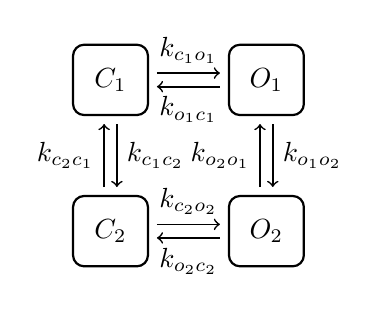
\begin{tikzpicture}[
   font=\sffamily,
   every matrix/.style={ampersand replacement=\&,column sep=1cm,row sep=1cm},
   state/.style={draw,thick,rounded corners,inner sep=.3cm},
   to/.style={->,semithick,shorten >=0.1cm,shorten <=0.1cm},
   Q/.style={->,semithick,sloped,pos=0.700000,shorten >=0.1cm,shorten <=0.1cm},  
   every node/.style={auto}]
\matrix{
\node[state] (C_{1}) {\parbox{10pt}{\centerline{$C_{1}$}}};\&\node[state] (O_{1}) {\parbox{10pt}{\centerline{$O_{1}$}}};\\
\node[state] (C_{2}) {\parbox{10pt}{\centerline{$C_{2}$}}};\&\node[state] (O_{2}) {\parbox{10pt}{\centerline{$O_{2}$}}};\\
};
\draw[to]  (C_{1}.10) to node {$k_{c_{1}o_{1}}$} (O_{1}.170);
\draw[to]  (C_{1}.280) to node {$k_{c_{1}c_{2}}$} (C_{2}.80);
\draw[to]  (O_{1}.190) to node {$k_{o_{1}c_{1}}$} (C_{1}.350);
\draw[to]  (O_{1}.280) to node {$k_{o_{1}o_{2}}$} (O_{2}.80);
\draw[to]  (C_{2}.100) to node {$k_{c_{2}c_{1}}$} (C_{1}.260);
\draw[to]  (C_{2}.10) to node {$k_{c_{2}o_{2}}$} (O_{2}.170);
\draw[to]  (O_{2}.100) to node {$k_{o_{2}o_{1}}$} (O_{1}.260);
\draw[to]  (O_{2}.190) to node {$k_{o_{2}c_{2}}$} (C_{2}.350);
\end{tikzpicture}
\end{center}
\caption{Markov model including four possible states: two open states, $O_{1}$ 
and $O_{2}$, and two closed states, $C_{1}$ and $C_{2}$.}%
\label{M44}%
\end{figure}

The probability density system associated with the model $(\ref{c1g})$ and $(\ref{c2g})$ when the Markov model is given by Figure \ref{M44} can now be 
written in the form%

\begin{align}
\frac{\partial\rho_{o_{1}}}{\partial t}+\frac{\partial}{\partial x}\left(
a_{o}^{x}\rho_{o_{1}}\right)  +\frac{\partial}{\partial y}\left(  a_{o}%
^{y}\rho_{o_{1}}\right)   &  =k_{c_{1}o_{1}}\rho_{c_{1}}-\left(  k_{o_{1}%
c_{1}}+k_{o_{1}o_{2}}\right)  \rho_{o_{1}}+k_{o_{2}o_{1}}\rho_{o_{2}%
},\nonumber\\
\frac{\partial\rho_{o_{2}}}{\partial t}+\frac{\partial}{\partial x}\left(
a_{o}^{x}\rho_{o_{2}}\right)  +\frac{\partial}{\partial y}\left(  a_{o}%
^{y}\rho_{o_{2}}\right)   &  =k_{c_{2}o_{2}}\rho_{c_{2}}-\left(  k_{o_{2}c_{2}%
}+k_{o_{2}o_{1}}\right)  \rho_{o_{2}}+k_{o_{1}o_{2}}\rho_{o_{1}}%
,\label{pdf44}\\
\frac{\partial\rho_{c_{1}}}{\partial t}+\frac{\partial}{\partial x}\left(
a_{c}^{x}\rho_{c_{1}}\right)  +\frac{\partial}{\partial y}\left(  a_{c}%
^{y}\rho_{c_{1}}\right)   &  =k_{o_{1}c_{1}}\rho_{o_{1}}-\left(  k_{c_{1}%
o_{1}}+k_{c_{1}c_{2}}\right)  \rho_{c_{1}}+k_{c_{2}c_{1}}\rho_{c_{2}%
},\nonumber\\
\frac{\partial\rho_{c_{2}}}{\partial t}+\frac{\partial}{\partial x}\left(
a_{c}^{x}\rho_{c_{2}}\right)  +\frac{\partial}{\partial y}\left(  a_{c}%
^{y}\rho_{c_{2}}\right)   &  =k_{c_{1}c_{2}}\rho_{c_{1}}-\left(  k_{c_{2}%
c_{1}}+k_{c_{2}o_{2}}\right)  \rho_{c_{2}}+k_{o_{2}c_{2}}\rho_{o_{2}%
},\nonumber
\end{align}
where %
\begin{align}
a_{o}^{x} &  =v_{r}\left(  y-x\right)  +v_{d}\left(  c_{0}-x\right)
,\nonumber\\
a_{o}^{y} &  =v_{r}\left(  x-y\right)  +v_{s}\left(  c_{1}-y\right)
,\label{flux44}\\
a_{c}^{x} &  =v_{d}\left(  c_{0}-x\right)  ,\nonumber\\
a_{c}^{y} &  =v_{s}\left(  c_{1}-y\right)  .\nonumber
\end{align}
By defining the states $O_{1},O_{2},C_{1},$ and $C_{2}$ to be the states 
1, 2, 3, and
4, respectively, we can write the system $(\ref{pdf44})$ in the more compact form%
\begin{equation}
\frac{\partial\rho_{i}}{\partial t}+\frac{\partial}{\partial x}\left(
a_{i}^{x}\rho_{i}\right)  +\frac{\partial}{\partial y}\left(  a_{i}^{y}%
\rho_{i}\right)  =\left(  K\rho\right)  _{i}\label{compact44}%
\end{equation}
for $i=1,2,3,4,$ where%
\begin{align*}
a_{i}^{x} &  =\gamma_{i}v_{r}\left(  y-x\right)  +v_{d}\left(  c_{0}-x\right)
,\\
a_{i}^{y} &  =\gamma_{i}v_{r}\left(  x-y\right)  +v_{s}\left(  c_{1}-y\right),
\end{align*}
and $\rho=(\rho_1,\rho_2,\rho_3,\rho_4)^T.$ 
Here $\gamma_{i}$ is one for the open states (i.e., $i=1$ and $i=2$) and zero for
the closed states (i.e., $i=3$ and $i=4$). Furthermore, the matrix is given by%
\[
K=\left(
\begin{array}
[c]{cccc}%
-\left(  k_{o_{1}c_{1}}+k_{o_{1}o_{2}}\right)   & k_{o_{2}o_{1}} &
k_{c_{1}o_{1}} & 0\\
k_{o_{1}o_{2}} & -\left(  k_{o_{2}c_{2}}+k_{o_{2}o_{1}}\right)   & 0 &
k_{c_{2}o_{2}}\\
k_{o_{1}c_{1}} & 0 & -\left(  k_{c_{1}o_{1}}+k_{c_{1}c_{2}}\right)   &
k_{c_{2}c_{1}}\\
0 & k_{o_{2}c_{2}} & k_{c_{1}c_{2}} & -\left(  k_{c_{2}c_{1}}+k_{c_{2}o_{2}%
}\right)
\end{array}
\right),
\]
which in compact notation is%
\[
K=\left(
\begin{array}
[c]{cccc}%
-\left(  k_{13}+k_{12}\right)   & k_{21} & k_{31} & 0\\
k_{12} & -\left(  k_{24}+k_{21}\right)   & 0 & k_{42}\\
k_{13} & 0 & -\left(  k_{31}+k_{34}\right)   & k_{43}\\
0 & k_{24} & k_{34} & -\left(  k_{43}+k_{42}\right)
\end{array}
\right)  .
\]

\bigskip
\section{Nine-state model}

We have seen how to formulate probability density systems for two-state and
four-state Markov models.  For even larger Markov models, it is useful to
introduce two-dimensional numbering. This will be illustrated using the nine-state model 
given in Figure \ref{ninestates}.%
\begin{figure}[ptb]
\begin{center}
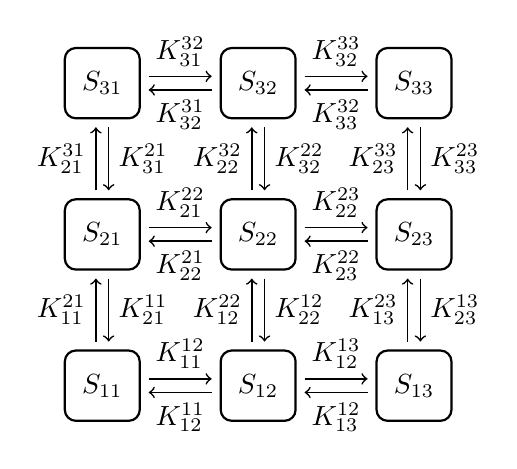
\begin{tikzpicture}[
   font=\sffamily,
   every matrix/.style={ampersand replacement=\&,column sep=1cm,row sep=1cm},
   state/.style={draw,thick,rounded corners,inner sep=.3cm},
   to/.style={->,semithick,shorten >=0.1cm,shorten <=0.1cm},
   Q/.style={->,semithick,sloped,pos=0.700000,shorten >=0.1cm,shorten <=0.1cm},  
   every node/.style={auto}]
\matrix{
\node[state] (S_{31}) {\parbox{10pt}{\centerline{$S_{31}$}}};\&\node[state] (S_{32}) {\parbox{10pt}{\centerline{$S_{32}$}}};\&\node[state] (S_{33}) {\parbox{10pt}{\centerline{$S_{33}$}}};\\
\node[state] (S_{21}) {\parbox{10pt}{\centerline{$S_{21}$}}};\&\node[state] (S_{22}) {\parbox{10pt}{\centerline{$S_{22}$}}};\&\node[state] (S_{23}) {\parbox{10pt}{\centerline{$S_{23}$}}};\\
\node[state] (S_{11}) {\parbox{10pt}{\centerline{$S_{11}$}}};\&\node[state] (S_{12}) {\parbox{10pt}{\centerline{$S_{12}$}}};\&\node[state] (S_{13}) {\parbox{10pt}{\centerline{$S_{13}$}}};\\
};
\draw[to]  (S_{31}.10) to node {$K_{31}^{32}$} (S_{32}.170);
\draw[to]  (S_{31}.280) to node {$K_{31}^{21}$} (S_{21}.80);
\draw[to]  (S_{32}.190) to node {$K_{32}^{31}$} (S_{31}.350);
\draw[to]  (S_{32}.10) to node {$K_{32}^{33}$} (S_{33}.170);
\draw[to]  (S_{32}.280) to node {$K_{32}^{22}$} (S_{22}.80);
\draw[to]  (S_{33}.190) to node {$K_{33}^{32}$} (S_{32}.350);
\draw[to]  (S_{33}.280) to node {$K_{33}^{23}$} (S_{23}.80);
\draw[to]  (S_{21}.100) to node {$K_{21}^{31}$} (S_{31}.260);
\draw[to]  (S_{21}.10) to node {$K_{21}^{22}$} (S_{22}.170);
\draw[to]  (S_{21}.280) to node {$K_{21}^{11}$} (S_{11}.80);
\draw[to]  (S_{22}.100) to node {$K_{22}^{32}$} (S_{32}.260);
\draw[to]  (S_{22}.190) to node {$K_{22}^{21}$} (S_{21}.350);
\draw[to]  (S_{22}.10) to node {$K_{22}^{23}$} (S_{23}.170);
\draw[to]  (S_{22}.280) to node {$K_{22}^{12}$} (S_{12}.80);
\draw[to]  (S_{23}.100) to node {$K_{23}^{33}$} (S_{33}.260);
\draw[to]  (S_{23}.190) to node {$K_{23}^{22}$} (S_{22}.350);
\draw[to]  (S_{23}.280) to node {$K_{23}^{13}$} (S_{13}.80);
\draw[to]  (S_{11}.100) to node {$K_{11}^{21}$} (S_{21}.260);
\draw[to]  (S_{11}.10) to node {$K_{11}^{12}$} (S_{12}.170);
\draw[to]  (S_{12}.100) to node {$K_{12}^{22}$} (S_{22}.260);
\draw[to]  (S_{12}.190) to node {$K_{12}^{11}$} (S_{11}.350);
\draw[to]  (S_{12}.10) to node {$K_{12}^{13}$} (S_{13}.170);
\draw[to]  (S_{13}.100) to node {$K_{13}^{23}$} (S_{23}.260);
\draw[to]  (S_{13}.190) to node {$K_{13}^{12}$} (S_{12}.350);
\end{tikzpicture}
\end{center}
\caption{Markov model including nine possible states.}%
\label{ninestates}%
\end{figure}
Here $S_{ij},$ $i,j=1,2,3$, denotes the states of the Markov model and
$K_{ij}^{mn}$ denotes\footnote{We use $K_{ij}$ as shorthand for $K_{i,j},$ but
we use the comma when an index of the form $j+1$ is needed, that is we write
$K_{i,j+1}.$} the reaction rate from the state $S_{ij}$ to the state $S_{mn}.$
The system governing the probability density functions of these states can be
written in the form%
\begin{equation}
\frac{\partial\rho_{ij}}{\partial t}+\frac{\partial}{\partial x}\left(
a_{ij}^{x}\rho_{ij}\right)  +\frac{\partial}{\partial y}\left(  a_{ij}^{y}%
\rho_{ij}\right)  =R_{ij},\label{pdf99}%
\end{equation}
where%
\begin{align*}
R_{ij}  & =K_{i,j+1}^{i,j}\rho_{i,j+1}+K_{i+1,j}^{i,j}\rho_{i+1,j}%
+K_{i,j-1}^{i,j}\rho_{i,j-1}+K_{i-1,j}^{i,j}\rho_{i-1,j}\\
& -\left(  K_{i,j}^{i,j+1}+K_{i,j}^{i+1,j}+K_{i,j}^{i,j-1}+K_{i,j}%
^{i-1,j}\right)  \rho_{i,j}.
\end{align*}
Here $\rho_{ij}$ denotes the probability density function of the state
$S_{ij}$ and we use the convention that $K_{ij}^{mn}=0$ for $i,j,m,n\notin%
\left\{  1,2,3\right\}  .$ We also have%
\begin{align*}
a_{ij}^{x} &  =\gamma_{ij}v_{r}\left(  y-x\right)  +v_{d}\left(
c_{0}-x\right)  ,\\
a_{ij}^{y} &  =\gamma_{ij}v_{r}\left(  x-y\right)  +v_{s}\left(
c_{1}-y\right)  ,
\end{align*}
where $\gamma_{ij}=1$ when the state $S_{ij}$ represents an open state and
$\gamma_{ij}=0$ when $S_{ij}$ represents a closed state.





\chapter{Calcium-induced calcium release \label{cicr}}



We started in Chapter \ref{Ca_release_1D} by assuming that the concentrations of the junctional sarcoplasmic reticulum (JSR) and the network sarcoplasmic reticulum (NSR) are identical and that the L-type current can be ignored and thus we studied a one-dimensional problem where the calcium concentration of the dyad was the only variable of interest. The model is illustrated in Figures \ref{cicr_1D} and \ref{geom1D}. Then, in Chapter  \ref{Ca_release_2D}, we extended the model to account for the varying concentrations in the dyad and the JSR, but we still ignored the effect of the voltage-gated L-type channels and kept the concentration of the cytosol and the NSR constant. The two-dimensional model is illustrated in Figures \ref{cicr_2D} and \ref{geom2D}. Our aim is now to include the effect of L-type channels. The L-type channels open and close depending on the transmembrane potential $V$, so the model will therefore be parameterized by $V$. The model is illustrated in Figures \ref{cicr_2D_V} and \ref{geomCa_V}.

It should be noted that we are still interested in the dynamics related to the dyad and not to the whole cell. We therefore keep the concentration of the cytosol and NSR constant and assume that the concentration of the extracellular space ($c_e$) only affects the concentration of the dyad through the voltage-gated L-type calcium channels (LCCs). In a whole-cell model, this would be different in many ways, but we shall not consider that topic here.

The state of a voltage-gated channel is governed by a Markov model where the transitions depend on the transmembrane potential (or voltage for short). If the electrical potential in the dyad is given by $V_{i}$
(intracellular potential) and the extracellular potential is given by $V_{e}%
$, we define the transmembrane potential to be%
\[
V=V_{i}-V_{e}.
\]

As a notational convention, we use the subscript $r$ to indicate that $\bar
{\gamma}_{r}$ models the open or closed state of the ryanodine receptor (RyR)
and the subscript $l$ in the term $\bar{\gamma}_{l}J_{l}$ is used to indicate 
that this is the flux through the LCC.

\begin{figure}
\centering\resizebox{0.9\linewidth}{!}{\winslow{2.5}{1.5}{8.5}{8}}
\caption{The figure is a modified version of Figure 1 (panel A) of Winslow et 
al. \cite{winslow2006} and illustrates the components involved in calcium-induced calcium release (CICR). In this chapter, we concentrate on the dynamics in the box surrounded by a thin red line. We assume that the concentrations of the cytosol, the NSR, and the extracellular domain 
represented by the T-tubule are kept constant and that inflow of calcium through the LCCs is governed by a voltage-dependent Markov model.
 \label{cicr_2D_V}}
\end{figure}


\newlength{\Oldarrayrulewidth}
\newcommand{\Cline}[2]{%
  \noalign{\global\setlength{\Oldarrayrulewidth}{\arrayrulewidth}}%
  \noalign{\global\setlength{\arrayrulewidth}{#1}}\cline{#2}%
  \noalign{\global\setlength{\arrayrulewidth}{\Oldarrayrulewidth}}}


\begin{figure}
[ptb]
\begin{center}
\begin{tabular}{c!{\vrule width 1pt}c!{\vrule width 1pt}c!{\vrule width 1pt}c} 
\Cline{1pt}{2-2}  
&& \multicolumn{2}{c}{} \\
& Extracellular, $c_e$ & \multicolumn{2}{c}{} \\
&&  \multicolumn{2}{c}{}\\ \noalign{\hrule height 1pt}  
&&& \\
Cytosol, $c_0$ & Dyad, $\bar{x}(t)$ & JSR, $\bar{y}(t)$ & NSR, $c_1$ \ \ \ \ \  \\
&&& \\ \noalign{\hrule height 1pt}
\end{tabular}
\caption{Sketch of a release unit. The cytosolic ($c_0$), NSR ($c_1$), and extracellular ($c_e$) calcium concentrations are  assumed to be constant, while the concentrations of the dyad and JSR are given by $\bar{x}=\bar{x}(t)$ and $\bar{y}=\bar{y}(t)$, respectively. Furthermore, we assume that the flux of calcium from the extracellular space to the dyad is voltage gated. Recall that $c_0\ll c_1$. }%
\label{geomCa_V}%
\end{center}
\end{figure}

\section[Stochastic release model parameterized by $V$]{Stochastic release model parameterized by the transmembrane potential}

\graytable{l}{
{|c|c|} \hline
$v_d $ & 1 $\rm{ms^{-1}}$\\ \hline
$v_r $ & 0.1 $\rm{ms^{-1}}$\\ \hline
$v_s $ & 0.01 $\rm{ms^{-1}}$\\ \hline
$c_0 $ & 0.1 $\rm{\mu M}$\\ \hline
$c_1 $ & 1000 $\rm{\mu M}$ \\ \hline
$c_e $ & 1800 $\rm{\mu M}$ \\ \hline
}{Values of parameters used in simulations in this chapter. 
%${\ }^*$Unless otherwise stated. 
\label{tab:param2DV}}



%}{Values of parameters used in 2D simulations based on the scheme (\ref{nc1},\ref{nc2}). \label{tab:param2D}}

In the models we have studied so far, a very basic building block has been
that, if $x_{0}$ denotes the concentration of a large reservoir of calcium and
$x=x(t)$ denotes the concentration of a small space connected to the reservoir,
then the concentration $x$ evolves according to the model%
\begin{equation}
x^{\prime}(t)=v\left(  x_{0}-x(t)\right),  \label{linflux}%
\end{equation}
where $v$ denotes the speed of diffusion between the two spaces. Here we assume that the concentration of the large reservoir, $x_0$, can be kept constant.  This model
can be extended to the case where the channel between the spaces can be either
closed or open:%
\begin{equation}
\bar{x}^{\prime}(t)=\bar{\gamma}(t)v\left(  x_{0}-\bar{x}(t)\right),
\label{s_linfux}%
\end{equation}
where $\bar{\gamma}$ is a random variable taking on two possible values, one
(open) and zero (closed). The stochastic release models studied above are derived by
gluing together pieces of models of exactly this type.

 In this chapter, one
additional effect is added: We now allow calcium to flow into the dyad
through the LCCs. This flow depends on both the
gradient of the concentration and of the electrical potential across the membrane
dividing the extracellular space and the dyad. 

The process illustrated in Figure \ref{geomCa_V} can be modeled as follows
\begin{align}
\bar{x}^{\prime} &  =\bar{\gamma}_{r}v_{r}\left(  \bar{y}-\bar{x}\right)
+v_{d}\left(  c_{0}-\bar{x}\right)  -\bar{\gamma}_{l}J_{l},\label{c1v}\\
\bar{y}^{\prime} &  =\bar{\gamma}_{r}v_{r}\left(  \bar{x}-\bar{y}\right)
+v_{s}\left(  c_{1}-\bar{y}\right)  .\label{c2v}%
\end{align}
This model is almost the same as the one we analyzed above (see  $(
\ref{c1})$ and $(\ref{c2})  $ on page \pageref{c1}). The new term is given by
$-\bar{\gamma}_{l}J_{l}$ and it models the inflow of calcium through the
LCCs. The function $\bar{\gamma}_{l}$ is governed by a Markov model and, as
usual, it takes on two values: zero (closed) and one (open). The Markov model
governing $\bar{\gamma}_{l}$ depends on the transmembrane potential $V$ and
the flux depends on $V,$ the extracellular calcium concentration $c_{e}$ and the dyad concentration $x=x(t).$ As above, $v_{r}$ denotes the rate of release
from the JSR to the dyad, $v_{d}$ denotes the speed of calcium diffusion from the dyad
to the cytosol, and $v_{s}$ denotes the speed of calcium diffusion from the NSR
 to the JSR.

The Markov model governing $\bar{\gamma}_{r}$ will be the same as above, but we need to 
introduce a Markov model governing $\bar{\gamma}_{l}$. We will also combine these Markov models
to simplify the introduction of a probability density formulation. Furthermore, we need to describe the electrochemical flux $J_{l}$.

\subsection{Electrochemical Goldman--Hodgkin--Katz (GHK) flux}

Consider Figure \ref{cicr_2D_V} and suppose that the membrane between the
T-tubule and the dyad has thickness $L.$ If the electrical field is
constant through the channel, the flux is given by%
\begin{equation}
J_{l}=\frac{D}{L}\frac{2F}{RT}\frac{x-c_{e}e^{-\frac{2FV}{RT}}}{1-e^{-\frac
{2FV}{RT}}}V, \label{GHK}
\end{equation}
\graytable{l}{
{|c|c|} \hline
$F$ & $96485.3$ C mol$^{-1}$\\ \hline
$R$ & $8.3145$ J mol$^{-1}$K$^{-1}$\\\hline
$T$ & 310 K\\\hline
$V_0$ & 13.357 mV\\ \hline 
$\frac{D}{L}$&0.02 ms$^{-1}$\\ \hline 
}{Parameters in (\ref{GHK}).\label{FRT}}
which is referred to as the GHK flux (see Keener and Sneyd \cite{KeenerSneyd}). Here $D$ is
Fick's diffusion constant, $F$ is Faraday's constant, $R$ is the gas constant,
and $T$ is the absolute temperature.
By defining%
\[
V_0=\frac{RT}{2F},%
\]
we have%
\begin{equation}
J_{l}=\frac{D}{L}\frac{x-c_{e}e^{-\frac{V}{V_0}}}{1-e^{-\frac{V}{V_0}}}\frac{V}{V_0},\label{fluxJ}%
\end{equation}
where $F,R,T$, and $V_0$ are given in Table \ref{FRT}.
%\[%
%\begin{tabular}
%[c]{ll}%
%$F$ & $96485.3$ C mol$^{-1}$\\
%$R$ & $8.3145$ J mol$^{-1}$K$^{-1}$\\
%$T$ & 310 K\\
%$V_0$ & 13.357 mV\\[1mm]
%$\frac{D}{L}$&0.02ms$^{-1}$
%\label{FRT}
%\end{tabular}
%\]

%\K{zzz Jeg pr\o ver \r{a} se p\r{a} enhetene her. 
%Hva er enhetene til D og L? Hvis det er $\text{dm}^{2}/(\text{ms})$ 
%og dm, f\r{a}r vel $J_l$ enhet $\mu \text{mol}/(\text{ms dm}^2)$ mens de andre leddene i
%(8.3) og (8.4) har enhet $\mu \text{mol}/(\text{ms dm}^3)$? 
%Men slik er det vel ikke? }
%\G{We only need to know the ratio, we have used $D/L = v_l = 0.02$/ms. The symbol $v_l$ is not used in the text, but perhaps it should.}

\subsection{Assumptions}

As for the model in Chapter  \ref{Ca_release_2D}, we will make the following assumptions for the parameters involved:
\begin{align}
 c_{1}&\gg c_{0} \, \mbox{ and } \, v_r,v_d,v_s >0,  \label{assumption1V} \\
 v_{d}v_{s}&\ge v_{r}^{2}.  \label{assumption2V}
\end{align}

\begin{comment}
In the present model the transmembrane potential is a parameter and we will assume that it satisfies the condition 
\begin{equation}
V\leqslant V_{0}\ln\left(  \frac{v_{r}+v_{d}}{c_{1}v_{r}+c_{0}v_{d}}%
c_{e}\right). \label{cond_V_200}%
\end{equation}
With the parameters used in our computations (see Table \ref{tab:param2DV}),  this condition implies
that we consider transmembrane potentials satisfying the condition
\begin{equation}
V\leqslant39.87\text{mV.}\label{cond_V_201}%
\end{equation}
\end{comment}


\subsection{Equilibrium potential}

\bigskip The electrochemical equilibrium over the membrane separating the
extracellular space and the dyad is characterized by
\[
J_{l}=0.
\]
In equilibrium, we must have
\[
x=c_{e}e^{-\frac{V}{V_0}},%
\]
so the equilibrium transmembrane potential is given by
\begin{equation}
V_{eq}=V_0 \ln\frac{c_{e}}{x}\label{V_eq}.%
\end{equation}
For this value of the transmembrane potential $V,$ the driving force $\, -\bar{\gamma}_{l}J_{l}$ in the
system (\ref{c1v}) and (\ref{c2v}) is zero even if the channel is open. It
should also be noted that the equilibrium transmembrane potential depends on
the concentration $x$ of the dyad and will therefore be a dynamic quantity. Here it is useful to 
recall that we regard $V$ as a parameter input to the system and not a part of the dynamics.

\bigskip

\subsection{Linear version of the flux}

We mentioned above that our modeling so far has been based on very simple
linear fluxes of the form given in $\left(  \ref{linflux}\right)  .$ In the
case we are considering now, the flux depends on both the difference in
concentration and the electrical potential over the membrane; see $\left(
\ref{fluxJ}\right)$.  A Taylor series expansion of the GHK flux can be written as%

\begin{equation}
J_{l}=\allowbreak\frac{D}{L}\left(  x-c_{e}\right)  +\frac{D}{2L}\left(
x+c_{e}\right)  \frac{V}{V_0} +O\left( \left( V\slash V_0\right)^{2}\right) \label{l_flux}%
\end{equation}
and, therefore, if $V=0,$ the flux is given by 
\[ 
J_{l}=\frac{D}{L}\left(
x-c_{e}\right)
\]
so the term $-\bar{\gamma}_{l}J_{l} $ has the form we used
in $\left(  \ref{s_linfux}\right) .$ This means that the electrochemical flux given by $\left(
\ref{fluxJ}\right)$ reduces to a purely concentration-based flux 
 when there is no difference in electrical potential across the membrane.

%\K{zzz Jeg klarer ikke \r{a} utlede denne Taylor-utviklingen. Skal det egentlig
%v\ae re $O(( \frac{V}{V_0})^{2})$ eller spiller ikke det noen rolle?}

\subsection{Markov models for CICR}

As discussed above, two Markov processes are involved in the CICR. We have seen that the gating of the release of
calcium from the sarcoplasmic reticulum to the dyad is given by the stochastic variable
$\bar{\gamma}_{r}=\bar{\gamma}_{r}(t)$, which is governed by the reaction
scheme%
\begin{equation}
C_{r}\underset{k_{co}^{r}}{\overset{k_{oc}^{r}}{\leftrightarrows}}O_{r}.
\label{m_r}%
\end{equation}
We recall here that $r$ is used to indicate the relation to the RyR
channels. Similarly, the Markov model for the LCC is given by%
\begin{equation}
C_{l}\underset{k_{co}^{l}}{\overset{k_{oc}^{l}}{\leftrightarrows}}O_{l},
\label{m_l}%
\end{equation}
where $l$ is used to indicate the relation to the LCCs.
This Markov model governs the stochastic variable $\bar{\gamma}_{l}%
=\bar{\gamma}_{l}(t).$

It is convenient to combine these two Markov models into one reaction scheme
of the form illustrated in Figure \ref{eq:m_rl}.%
\begin{figure}[ptb]
\begin{center}
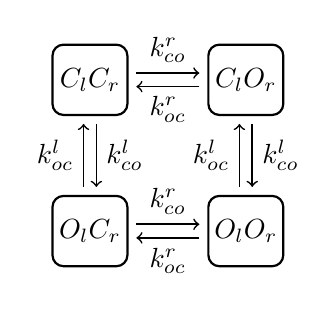
\begin{tikzpicture}[
   font=\sffamily,
   every matrix/.style={ampersand replacement=\&,column sep=1cm,row sep=1cm},
   state/.style={draw,thick,rounded corners,inner sep=.3cm},
   to/.style={->,semithick,shorten >=0.1cm,shorten <=0.1cm},
   Q/.style={->,semithick,sloped,pos=0.700000,shorten >=0.1cm,shorten <=0.1cm},  
   every node/.style={auto}]
\matrix{
\node[state] (C_{l}C_{r}) {\parbox{10pt}{\centerline{$C_{l}C_{r}$}}};\&\node[state] (C_{l}O_{r}) {\parbox{10pt}{\centerline{$C_{l}O_{r}$}}};\\
\node[state] (O_{l}C_{r}) {\parbox{10pt}{\centerline{$O_{l}C_{r}$}}};\&\node[state] (O_{l}O_{r}) {\parbox{10pt}{\centerline{$O_{l}O_{r}$}}};\\
};
\draw[to]  (C_{l}C_{r}.10) to node {$k_{co}^{r}$} (C_{l}O_{r}.170);
\draw[to]  (C_{l}C_{r}.280) to node {$k_{co}^{l}$} (O_{l}C_{r}.80);
\draw[to]  (C_{l}O_{r}.190) to node {$k_{oc}^{r}$} (C_{l}C_{r}.350);
\draw[to]  (C_{l}O_{r}.280) to node {$k_{co}^{l}$} (O_{l}O_{r}.80);
\draw[to]  (O_{l}C_{r}.100) to node {$k_{oc}^{l}$} (C_{l}C_{r}.260);
\draw[to]  (O_{l}C_{r}.10) to node {$k_{co}^{r}$} (O_{l}O_{r}.170);
\draw[to]  (O_{l}O_{r}.100) to node {$k_{oc}^{l}$} (C_{l}O_{r}.260);
\draw[to]  (O_{l}O_{r}.190) to node {$k_{oc}^{r}$} (O_{l}C_{r}.350);
\end{tikzpicture}
\end{center}
\caption{Markov model including four possible states: $C_{l}C_{r}$ (both
closed), $C_{l}O_{r}$ (LCC closed, RyR open), $O_{l}O_{r}$ (both open), and
$O_{l}C_{r}$ (LCC open, RyR closed).}%
\label{eq:m_rl}%
\end{figure}
The states of this combined Markov model are given by $C_{l}C_{r}$ (both
closed), $C_{l}O_{r}$ (LCC closed, RyR open), $O_{l}O_{r}$ (both open), and
$O_{l}C_{r}$ (LCC open, RyR closed). In our computations, we use the rates shown in Table \ref{tab:rate}.
%following functions%
%\begin{equation}%
\begin{table}
\begin{center}
%\begin{tabular}[c]{|l|l|l|l|} \hline
%$k_{co}^{r}=\mu \frac{x^4}{K(y)^4+x^4}$ & $k_{oc}^{r}=1$ & 
%$K(y) =  K_{max}-y/1000$ & $K_{max} = 7.4\mu$M \\ \hline
%$k_{co}^{l}=\eta\, l_{\infty}(V)/\tau_l$ & $k_{oc}^{l}=(1-l_{\infty}(V))/\tau_l%$ &$l_{\infty}(V) = 0.01 \exp(-(V-5)^2/500)$ 
%&$\tau_l=1$ms \\ \hline
\begin{tabular}[c]{|l|l|} \hline
RyR: & LCC: \\
$k_{co}^{r}=\mu \frac{x^4}{K(y)^4+x^4} \text{ ms}^{-1}$ &$k_{co}^{l}=\eta\, l_{\infty}(V)/\tau_l$ \\
$k_{oc}^{r}=1 \text{ ms}^{-1}$ & $k_{oc}^{l}=(1-l_{\infty}(V))/\tau_l$ \\
$K(y) =  K_{max}-y/1000$ &  $l_{\infty}(V) = 0.01 \exp(-(V-5)^{2}/500)$ \\
$K_{max} = 7.4$ $\mu$M & $\tau_l=1$ ms\\ \hline
\end{tabular}
\end{center}
%\end{equation}
\caption{Reaction rates used in the Markov model illustrated in 
Figure \ref{eq:m_rl}.
 Here $\mu \ge 1$ denotes the mutation severity
index of the RyR, $\eta \ge 1$ denotes the mutation severity
index of the LCC and $\mu=\nu=1$ represents the wild type case. 
\label{functions}
\label{tab:rate}}
\end{table}

\subsection{Numerical scheme for the stochastic CICR  model}

 A numerical scheme for running simulations based on the CICR model 
($\ref{c1v}$) and ($\ref{c2v}$)
is given by
\begin{align}
x_{n+1} &  =x_{n}+\Delta t\left(  \gamma_{n}^{r}v_{r}\left(  y_{n}%
-x_{n}\right)  +v_{d}\left(  c_{0}-x_{n}\right)  \right)  -\Delta t \gamma_{n}^{l}%
J_{l}(x_{n},V),\label{nc1v}\\
y_{n+1} &  =y_{n}+\Delta t\left(  \gamma_{n}^{r}v_{r}\left(  x_{n}%
-y_{n}\right)  +v_{s}\left(  c_{1}-y_{n}\right)  \right)  ,\label{nc2v}%
\end{align}
where $\gamma_{n}^{r}$ and $\gamma_{n}^{l}$ are computed according to the
Markov model illustrated in Figure \ref{eq:m_rl}.

\subsection{Monte Carlo simulations of CICR}

In Figure \ref{cicr/cicr.pdf}, we show the results of stochastic simulations 
using the model $(\ref{c1v})$ and $(\ref{c2v}) $. 
The computations are based on the numerical scheme 
$(\ref{nc1v})$  and $(\ref{nc2v}) $ with the parameters given in Table \ref{tab:param2DV} and $\Delta t=0.01$ ms. As initial conditions we have used $x(0) = c_0$ and $y(0) = c_1$ with both gates closed.
From top to bottom, the transmembrane potential is given by $V=20$ mV, $0$ mV, $-20$ mV, and $-40$ mV. 

The associated calcium concentrations of the dyad given by $x=x(t)$ are graphed in the left panels and the 
calcium concentrations of the JSR given by $y=y(t)$ are graphed in the right panels. 
In all cases, we show the solution for a time interval ranging from 0 ms to 1000 ms. 
The calcium concentration clearly depends on the transmembrane potential and we observe in particular that there
is no activity for $V=-40$ mV, since the LCC is inactivated at that voltage. 

In Figure \ref{cicr/zoom.pdf}, we show a detailed view of the case of $V=0$ mV. 
In the upper part of the graph we show the state
of the RyR (upper) and the LCCs (lower). The CICR mechanism is illustrated in the first part of the graph: The LCC opens at $t \approx 5$ ms, but the release is too short-lived to trigger an RyR opening and we therefore observe just a minor increase in the dyad calcium concentration given by  $x$. Next time, at 
$t \approx 9$ ms, there is a new opening and now the channel is open for a longer time;
there is an increase in $x$ leading to opening of the RyR channel and then the concentration increases dramatically.

\fig{cicr/cicr.pdf}{Calcium dynamics of the dyad $x=x(t)$ and the JSR $y=y(t)$ for four values of the transmembrane potential $V$.
}
\fig{cicr/zoom.pdf}{A detailed view of the case of $V=0$ mV taken from Figure \ref{cicr/cicr.pdf}. In addition, we show
the state of the RyR channel (upper panel) and the LCC (lower panel).
The first spike at 5 ms in the LCC is very short and does not trigger an RyR release. 
The next one, at 9 ms, does trigger an RyR release.}


%\begin{table}[ptb]
%\begin{center}%
%\begin{tabular}
%[c]{|l|l||l|l|}\hline
%$v_{r}$ & 0.1/ms & $c_{0}$ & 0.1$\mu$M \\\hline
%$v_{d}$ & 1/ms & $c_{1}$ & 1000$\mu$M \\\hline
%$v_{s}$ & 0.01/ms &  & \\\hline
%$k_{oc}$ &  & $k_{co}$ & \\\hline
%\end{tabular}
%\end{center}
%\caption{Values of parameters used in simulations. }%
%\label{tab:param2DV}%
%\end{table}

\section{Invariant region for the CICR model}

We have seen in both the one- and two-dimensional models above that we can derive invariant
regions for the stochastic models and that these regions define the
computational domain for the probability density system. Our aim is now to
derive an invariant region for the CICR model given by%
\begin{align}
\bar{x}^{\prime}  &  =\bar{\gamma}_{r}v_{r}\left(  \bar{y}-\bar{x}\right)
+v_{d}\left(  c_{0}-\bar{x}\right)  -\bar{\gamma}_{l}J_{l},\label{c1v2}\\
\bar{y}^{\prime}  &  =\bar{\gamma}_{r}v_{r}\left(  \bar{x}-\bar{y}\right)
+v_{s}\left(  c_{1}-\bar{y}\right)  . \label{c2v2}%
\end{align}
Here it is convenient to write the GHK flux in the form%
\[
J_{l}(x)=a_{0}(x-x_{0}),
\]
where%
\[
a_{0}=\frac{D}{L}\frac{1}{1-e^{-\frac{V}{V_{0}}}}\frac{V}{V_{0}}%
\]
and%
\[
x_{0}=c_{e}e^{-\frac{V}{V_{0}}},
\]
so the system takes the form%
\begin{align}
\bar{x}^{\prime}  &  =\bar{\gamma}_{r}v_{r}\left(  \bar{y}-\bar{x}\right)
+v_{d}\left(  c_{0}-\bar{x}\right)  +\bar{\gamma}_{l}a_{0}(x_{0}-\bar
{x}),\label{xc1v2}\\
\bar{y}^{\prime}  &  =\bar{\gamma}_{r}v_{r}\left(  \bar{x}-\bar{y}\right)
+v_{s}\left(  c_{1}-\bar{y}\right)  . \label{yc2v2}%
\end{align}


\subsection{A numerical scheme}

Let us consider the numerical scheme (\ref{nc1v}, \ref{nc2v}), 
\begin{align}
x_{n+1}  &  =x_n+\Delta t\left( \gamma_n^{r}v_{r}\left(  y-x\right)  +v_{d}\left(
c_{0}-x\right)  +\gamma_n^{l}a_{0}(x_{0}-x)\right) ,\label{x400}\\
y_{n+1} &  =y_n+\Delta t\left(\gamma_n^{r}v_{r}\left(  x-y\right)  +v_{s}\left(
c_{1}-y\right) \right)  . \label{y400}%
\end{align}
Here $\gamma_n^{r}$ and $\gamma_n^{l}$ simply denotes constants that take on the
value zero or one and their values will be specified in order to study the
dynamics of the system when the associated channels are open or closed. The
numerical scheme can be written in the form%
\begin{align}
x_{n+1} &  =F\left(  x_{n},y_{n}\right)  ,\label{x401}\\
y_{n+1} &  =G\left(  x_{n},y_{n}\right)  ,\label{y401}%
\end{align}
with%
\begin{align*}
F(x,y) &  =x+\Delta t\left(  \gamma_{r}v_{r}\left(  y-x\right)  +v_{d}\left(
c_{0}-x\right)  +\gamma_{l}a_{0}(x_{0}-x)\right)  ,\\
G(x,y) &  =y+\Delta t\left(  \gamma_{r}v_{r}\left(  x-y\right)  +v_{s}\left(
c_{1}-y\right)  \right).
\end{align*}
Here we assume that
\begin{equation}
\Delta t\leqslant\min\left(  \frac{1}{v_{d}+a_{0}+v_{r}},\frac{1}{v_{s}+v_{r}%
}\right).  \label{dt400}%
\end{equation}
Under this condition, we observe that%
\[
\frac{\partial F}{\partial x}=1-\Delta t\left(  v_{d}+\gamma_{l}a_{0}%
+\gamma_{r}v_{r}\right)  \geqslant0
\]
for any choice of $\gamma_{l}$ and $\gamma_{r}$. We also have%
\[
\frac{\partial F}{\partial y}=\Delta t \gamma_{r}v_{r}\geqslant0.
\]
Similarly, we find that
\begin{equation}
\frac{\partial G}{\partial x}=\Delta t \gamma_{r}v_{r}\geqslant0
\end{equation}
and%
\begin{equation}
\frac{\partial G}{\partial y}=1-\Delta t\left(  v_{s}+\gamma_{r}v_{r}\right)
\geqslant0.
\end{equation}
Assume that%
\begin{equation}
0\leqslant x_{n},y_{n}\leqslant M,\label{y411}%
\end{equation}
where%
\[
M=\max\left(  c_{1},\frac{c_0 v_d +a_{0}x_{0}}{a_{0}+v_{d}}\right)  .
\]
Since
\[
\frac{\partial F}{\partial x},\frac{\partial F}{\partial y},\frac{\partial
G}{\partial x},\frac{\partial G}{\partial y}\geqslant0,
\]
we have%
\[
x_{n+1}=F\left(  x_{n},y_{n}\right)  \leqslant F(M,M)=M+\Delta t\left(
v_{d}\left(  c_{0}-M\right)  +\gamma_{l}a_{0}(x_{0}-M)\right)  \leqslant M
\]
and%
\[
y_{n+1}=G\left(  x_{n},y_{n}\right)  \leqslant G(M,M)=M+\Delta t\left(
v_{s}\left(  c_{1}-M\right)  \right)  \leqslant M.
\]
Furthermore, we have%
\[
x_{n+1}=F\left(  x_{n},y_{n}\right)  \geqslant F(0,0)=\Delta t\left(
v_{d}c_{0}+\gamma_{l}a_{0}x_{0}\right)  \geqslant0
\]
and%
\[
y_{n+1}=G\left(  x_{n},y_{n}\right)  \geqslant G(0,0)=\Delta tv_{s}%
c_{1}\geqslant0.
\]
So, by induction, the invariant region $\left(  \ref{y411}\right)$ holds for
all $n\geqslant0.$


\section[Probability density model parameterized by V]{Probability density model parameterized by the transmembrane potential}


The probability density formulation of the system ($\ref{c1v}$) and ($\ref{c2v}$) is given by the
 system of partial differential equations
\begin{align}
\frac{\partial\rho_{oo}}{\partial t}+\frac{\partial}{\partial x}\left(
a_{oo}^{x}\rho_{oo}\right)  +\frac{\partial}{\partial y}\left(  a_{oo}^{y}%
\rho_{oo}\right)   &  =k_{co}^{l}\rho_{co}-\left(  k_{oc}^{l}+k_{oc}%
^{r}\right)  \rho_{oo}+k_{co}^{r}\rho_{oc},\label{eq:pdfoo}\\
\frac{\partial\rho_{oc}}{\partial t}+\frac{\partial}{\partial x}\left(
a_{oc}^{x}\rho_{oc}\right)  +\frac{\partial}{\partial y}\left(  a_{oc}^{y}%
\rho_{oc}\right)   &  =k_{co}^{l}\rho_{cc}-\left(  k_{oc}^{l}+k_{co}%
^{r}\right)  \rho_{oc}+k_{oc}^{r}\rho_{oo},\label{eq:pdfoc}\\
\frac{\partial\rho_{cc}}{\partial t}+\frac{\partial}{\partial x}\left(
a_{cc}^{x}\rho_{cc}\right)  +\frac{\partial}{\partial y}\left(  a_{cc}^{y}%
\rho_{cc}\right)   &  =k_{oc}^{l}\rho_{oc}-\left(  k_{co}^{l}+k_{co}%
^{r}\right)  \rho_{cc}+k_{oc}^{r}\rho_{co},\label{eq:pdfcc}\\
\frac{\partial\rho_{co}}{\partial t}+\frac{\partial}{\partial x}\left(
a_{co}^{x}\rho_{co}\right)  +\frac{\partial}{\partial y}\left(  a_{co}^{y}%
\rho_{co}\right)   &  =k_{oc}^{l}\rho_{oo}-\left(  k_{co}^{l}+k_{oc}%
^{r}\right)  \rho_{oc}+k_{co}^{r}\rho_{cc},\label{eq:pdfco}%
\end{align}
where $\rho_{oo},\rho_{oc},\rho_{cc},$ and $\rho_{co}$ represent the probability
densities of the states denoted 
$O_{l}O_{r},O_{l}C_{r},C_{l}C_{r},$ and $C_{l}O_{r},$ respectively. The terms of the fluxes are given by%
\[
\begin{tabular}
[c]{ll}%
$a_{oo}^{x}=v_{r}\left(  y-x\right)  +v_{d}\left(  c_{0}-x\right)
-J_{l}(x,V),$ & $a_{oo}^{y}=v_{r}\left(  x-y\right)  +v_{s}\left(
c_{1}-y\right),  $\\
$a_{oc}^{x}=v_{d}\left(  c_{0}-x\right) - J_{l}(x,V),$ &
$a_{oc}^{y}=v_{s}\left(  c_{1}-y\right),  $\\
$a_{cc}^{x}=v_{d}\left(  c_{0}-x\right),  $ & $a_{cc}^{y}=v_{s}\left(
c_{1}-y\right),  $\\
$a_{co}^{x}=v_{r}\left(  y-x\right)+v_{d}\left(  c_{0}-x\right),  $ & $a_{co}^{y}%
=v_{r}\left(  x-y\right)  +v_{s}\left(  c_{1}-y\right),  $%
\end{tabular}
\]
where we use the convention that in the expression $a_{\alpha\beta}%
^{x},$ the index $\alpha$ indicates whether the LCC is open
$(\alpha=o)$ or closed $(\alpha=c)$ and the index $\beta$ plays the same role
for the RyR channel. Similar notation is used for the flux terms represented by
$a_{\alpha\beta}^{y}.$ As usual, the sum of total probabilities is 
one:%
\begin{equation}
\int_{\Omega}\left(  \rho_{oo}+\rho_{oc}+\rho_{cc}+\rho_{co}\right)  dx\,dy=1. \label{sumone}
\end{equation}



\section{Computing probability density representations of CICR}

 In Figure \ref{cicr/Vdep.pdf}, we show solutions of the system ($\ref{c1v2}$) and ($\ref{c2v2}$) defined in the computational domain 
 $\Omega=\Omega(V)$ for four values of the transmembrane potential: $V = 20$ mV, $0$ mV, $-20$ mV, and $-40$ mV. In all computations, the parameters are given in Table \ref{tab:param2DV} and the Markov model is illustrated in Figure \ref{eq:m_rl}. 
All distributions are initially set to zero, except that $\rho_{cc}(c_0,c_1)= 1/(\Delta x \Delta y)$. Hence the initial discrete probability densities integrates to one;
\begin{equation}
\Delta x \Delta y \sum_{i,j}  \rho_{i,j}=1,  % \label{discrete_sumone}
\end{equation}
which is a discrete version of $(\ref{sumone})$ with $\rho=\rho_{oo}+\rho_{oc}+\rho_{co}+\rho_{cc}$.  

The simulation results are shown in Figure \ref{cicr/Vdep.pdf}  and summarized in Table \ref{tab:stat2DV}. We observe that the transmembrane potential $V$ significantly influences the probability density functions. In Table \ref{tab:stat2DV}, we observe that the probability of the LCC being in the open state is highest for $V=0$ mV and it is almost zero for $V=-40$ mV. In the computations, we use $\Delta t=0.001$ ms, $\Delta x=1.02$ $\mu$M, $1.23$ $\mu$M, $1.54$ $\mu$M and $1.95$ $\mu$M (the domain size varies with $V$), and $\Delta y=9.3$ $\mu$M. Note that the scale of the plots varies (see Figure \ref{cicr/Vdep.pdf}).


\fig{cicr/Vdep.pdf}{Probability density functions for different voltages. The LCC is more prone to being open (last two columns) when the voltage is close to $V=5$ mV, that is, where $l_{\infty}(V)$ is close to its maximum. Black corresponds to $10^{-3}$ for $\rho_{cc}$ and to $10^{-6}$ for the other three distributions.}

\begin{table}  \begin{center}
\begin{tabular}{|r|r|r|r|r|} \hline
 $V$ & $\pi_{cc}$ & $\pi_{co}$ & $\pi_{oc}$ & $\pi_{oo}$ \\ \hline
20 & 0.978 & 0.015 & 0.005 & 0.001 \\ \hline
0 & 0.959 & 0.032 & 0.007 & 0.003 \\ \hline
-20 & 0.982 & 0.015 & 0.002 & 0.001 \\ \hline
-40 & 0.993 & 0.006 & 0.000 & 0.000 \\ \hline
\end{tabular} \end{center}
\caption{Probability of being in the four states for different voltages. Recall that the probabilities are computed
using  (\ref{probability}) at page \pageref{probability} where the probability density functions are numerical solutions
of the system (\ref{eq:pdfoo})-(\ref{eq:pdfco}).}
\label{tab:stat2DV}
\end{table}




\section{Effects of LCC and RyR mutations}

We are now in a position to study the effect of both LCC and RyR mutations. We
assume that both the LCC and RyR mutations lead to leaky channels that can be
represented by increasing the reaction rate from closed to open. So we again consider CO-mutations. 

The reaction scheme in the presence of mutations is illustrated in Figure \ref{Eq:m_rl_m}.
Here $\mu\geq1$ denotes the
strength of the RyR mutations and $\eta\geq1$ denotes the strength of the LCC
mutations. Note that $\mu=1$ and $\eta=1$ represent the wild type.

\begin{figure}[ptb]
\begin{center}
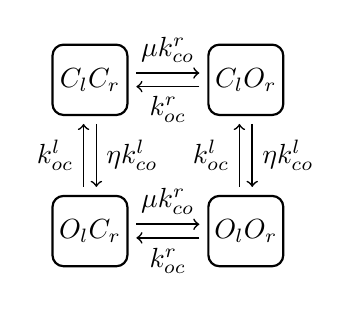
\begin{tikzpicture}[
   font=\sffamily,
   every matrix/.style={ampersand replacement=\&,column sep=1cm,row sep=1cm},
   state/.style={draw,thick,rounded corners,inner sep=.3cm},
   to/.style={->,semithick,shorten >=0.1cm,shorten <=0.1cm},
   Q/.style={->,semithick,sloped,pos=0.700000,shorten >=0.1cm,shorten <=0.1cm},  
   every node/.style={auto}]
\matrix{
\node[state] (C_{l}C_{r}) {\parbox{10pt}{\centerline{$C_{l}C_{r}$}}};\&\node[state] (C_{l}O_{r}) {\parbox{10pt}{\centerline{$C_{l}O_{r}$}}};\\
\node[state] (O_{l}C_{r}) {\parbox{10pt}{\centerline{$O_{l}C_{r}$}}};\&\node[state] (O_{l}O_{r}) {\parbox{10pt}{\centerline{$O_{l}O_{r}$}}};\\
};
\draw[to]  (C_{l}C_{r}.10) to node {$\mu k_{co}^{r}$} (C_{l}O_{r}.170);
\draw[to]  (C_{l}C_{r}.280) to node {$\eta k_{co}^{l}$} (O_{l}C_{r}.80);
\draw[to]  (C_{l}O_{r}.190) to node {$k_{oc}^{r}$} (C_{l}C_{r}.350);
\draw[to]  (C_{l}O_{r}.280) to node {$\eta k_{co}^{l}$} (O_{l}O_{r}.80);
\draw[to]  (O_{l}C_{r}.100) to node {$k_{oc}^{l}$} (C_{l}C_{r}.260);
\draw[to]  (O_{l}C_{r}.10) to node {$\mu k_{co}^{r}$} (O_{l}O_{r}.170);
\draw[to]  (O_{l}O_{r}.100) to node {$k_{oc}^{l}$} (C_{l}O_{r}.260);
\draw[to]  (O_{l}O_{r}.190) to node {$k_{oc}^{r}$} (O_{l}C_{r}.350);
\end{tikzpicture}
\end{center}
\caption{Mutant version of the Markov model given in Figure \ref{eq:m_rl}
including four possible states: $C_{l}C_{r}$ (both
closed), $C_{l}O_{r}$ (LCC closed, RyR open), $O_{l}O_{r}$ (both open), and
$O_{l}C_{r}$ (LCC open, RyR closed).}%
\label{Eq:m_rl_m}%
\end{figure}
 
 

\subsection{Effect of mutations measured in a norm}

To
measure the effect of the mutations, we introduce the norm
\begin{equation}
\Vert \rho^{\eta,\mu}-\rho^{1,1}\Vert=\frac{1}{6}\sum_{V} \sum_{z}\frac{\Vert\rho_z^{\eta,\mu}-\rho_z^{1,1}\Vert_{L^{2}\left(  \Omega\right)  }}{\Vert\rho_z^{\eta,\mu}\Vert_{L^{2}\left(  \Omega\right)}+\Vert\rho_z^{1,1}\Vert_{L^{2}\left(  \Omega\right)}, \label{norm44}}
\end{equation}
where $\rho_z$ represents $\rho_{oo}$,$\, \rho_{oc}$,$\, \rho_{co}$, or
$\rho_{cc}$ and $V$ represents summation over the following values of the transmembrane potential: $-80$ mV, $-60$ mV, $-40$ mV, $-20$ mV, $0$ mV, and $20$ mV. Furthermore, %
\begin{equation}
\Vert\rho\Vert_{L^{2}\left(  \Omega\right)  }=\left(\int_{\Omega}\rho^2 d\Omega\right) ^{1/2}. \label{norm_rho}
\end{equation}


The difference between the wild type solution and the solution based on
mutated reaction rates is depicted in Figure \ref{cicr/mutations.pdf}. 
The figure shows the difference as a function of the two mutation severity indices $\mu$ and $\eta$. 


\fig{cicr/mutations.pdf}{Difference between wild type solutions and mutated solutions, defined in terms of the norm given by (\ref{norm44}). The wild type solution is represented by $\mu=\eta=1$.}



\subsection{Mutations increase the open probability of both the LCC and RyR channels}

In Section \ref{statistics} (page \pageref{statistics}), we introduced statistical measures for the probability density functions. We will now consider how the LCC and RyR mutations affect the statistical properties of the associated probability density functions. Let us first consider how the mutations affect the total probability of being in the different states. In Figure \ref{cicr/mut_I.pdf}, we show the total probability of being in the states OO, CO, OC, and CC, where, as above, the first letter denotes the state of the LCC and the second letter indicates the state of the RyR channel. Here the value of the transmembrane potential is $V=0$ mV. 
In  Figure \ref{cicr/mut_IV80.pdf}, we show similar results in the case of $V=-80$ mV; the probability of the LCC being open is very small and the LCC mutation must be extremely severe to change this. Basically, at $V=-80$ mV, the LCC is closed independent of the mutations. This observation certainly depends heavily on the particular reaction rates used in these computations (see Table (\ref{functions}) on page \pageref{functions}).



\fig{cicr/mut_I.pdf}{Probability of being in the state OO, CO, OC, or CC at $V=0$ mV
as a function of the mutation severity index of the LCC, represented by $\eta$, and the
mutation severity index of the RyR channel, represented by $\mu$. Here $\eta=\mu=1$ represents the wild type. }
\fig{cicr/mut_IV80.pdf}{Probability of being in the state OO, CO, OC, or CC at $V=-80$ mV
as a function of the mutation severity index of the LCC, represented by $\eta$, and the
mutation severity index of the RyR channel, represented by $\mu$. Here $\eta=\mu=1$ represents the wild type.
Note the scale of the axis in the plots on the left-hand side.}




\subsection{Mutations change the expected values of concentrations}

 Figures \ref{cicr/mut_XY.pdf} and \ref{cicr/mut_XYV80.pdf} show the development of the expected concentration for varying strengths of mutations. In Figure \ref{cicr/mut_XY.pdf}, we set $V=0$ mV and see that the mutations change the expected concentrations significantly. More specifically, both mutations lead to lower expected JSR concentrations. In Figure \ref{cicr/mut_XYV80.pdf}, we set $V=-80$ mV and observe that the expected concentrations are not altered by the LCC mutation. As for the total probabilities discussed above, the reason for this is that, at this value of $V$, the probability of going from closed to open is practically zero and the mutation must be orders of magnitude larger to open the LCC at this voltage. Again, this observation is based on the particular form of the reaction rates given in Table \ref{functions}.

\fig{cicr/mut_XY.pdf}{This figure shows how the expected concentrations of the dyad (given by $x$) and the JSR (given by $y$) change as functions of the mutation severity indices. The curve denoted by $E_{cc}$ starts at the circle that represents the expected values of $x$ and $y$ in the case of both the LCC and RyR being closed. The starting point represents the wild type and the curves represent the two mutations (or combinations of them) and similarly for the curves starting at the circles next to $E_{oc}$,\, $E_{co}$, and $E_{oo}$. All curves are computed using $V=0$ mV.}

\fig{cicr/mut_XYV80.pdf}{This figure shows how the expected concentrations of the dyad (given by $x$) and the JSR (given by $y$) change as functions of the mutation severity indices. The curve denoted by $E_{cc}$ starts at the circle that represents the expected values of $x$ and $y$ in the case of both LCC and RyR being closed. The starting point represents the wild type and the curves represent the two mutations (or combinations of them) and similarly for the curves starting at the circles next to $E_{oc}$,\, $E_{co}$, and $E_{oo}$. All curves are computed using $V=-80$ mV.}



\section{Notes}
\begin{enumerate}
\item The Markov model  (including parameters)  given in Figure \ref{eq:m_rl} and the probability density system  $(  \ref{eq:pdfoo})$--$(\ref{eq:pdfco})  $
 are taken from Williams et al. \cite{Williams2007}.
\item The functions given in Table (\ref{functions}) are motivated by the models of Stern et al. \cite{Stern1999}.
\end{enumerate}

\chapter[Numerical drugs for CICR]{Numerical drugs for calcium-induced calcium release}



\graytable{l}{
{|c|c|} \hline
$v_d $ & 1 $\rm{ms^{-1}}$\\ \hline
$v_r $ & 0.1 $\rm{ms^{-1}}$\\ \hline
$v_s $ & 0.01 $\rm{ms^{-1}}$\\ \hline
$c_0 $ & 0.1 $\rm{\mu M}$\\ \hline
$c_1 $ & 1000 $\rm{\mu M}$ \\ \hline
}{Values of parameters used in simulations in this chapter. 
\label{tab:cicr_again}}


In the previous chapter, we developed models of calcium-induced calcium release (CICR) in terms of both a stochastic release model and a model of the probability density functions of the states involved in the stochastic release model. The models incorporated the effects of mutations in both the ryanodine receptors (RyRs) and the L-type calcium channels (LCCs).
The purpose of the present chapter is to introduce theoretical drugs aimed at repairing the effect of mutations of both the LCCs and RyR channels. 

We have seen in previous chapters that, if we ignore the effect of the LCC, we can completely repair the effect of an RyR mutation using a closed state blocker if the mutation is of the CO type. In this chapter, we want to see if this result also holds when the effect of the LCCs is taken into account. Since the transmembrane potential $V$ enters the model as a parameter, it is sufficient to control the effect of the LCCs for a number of different values of $V$.
The next issue we want to address is how to repair the effect of LCC mutations. 
We will find optimal open and closed state blockers. 
%Although somewhat unconventional, we will also try to use an LCC blocker to repair RyR mutations and vice versa. 

\section{Markov models for CICR, including drugs}

We consider a situation where the RyR or the LCC may be affected by CO-mutations. Both effects are modeled by Markov models and in this section we introduce theoretical drugs in terms of open and closed state blockers for both the RyR and the LCC.

\subsection{Theoretical blockers for the RyR}

As discussed above, the gating of the release of calcium from the sarcoplasmic reticulum to the dyad is
given by the stochastic variable $\bar{\gamma}_{r}=\bar{\gamma}_{r}(t)$
governed by the reaction scheme%
\begin{equation}
C_{r}\underset{\mu k_{co}^{r}}{\overset{k_{oc}^{r}}{\leftrightarrows}}%
O_{r}.\label{m_r2}%
\end{equation}
Here $\mu$ is the mutation severity index, which is one in the wild type case. 
We have seen that open and closed state blockers can be added to the reaction as%
\begin{equation}
B_{c}^{r}\underset{k_{bc}^{r}}{\overset{k_{cb}^{r}}{\leftrightarrows}}%
C_{r}\underset{\mu k_{co}^{r}}{\overset{k_{oc}^{r}}{\leftrightarrows}}%
O_{r}\underset{k_{ob}^{r}}{\overset{k_{bo}^{r}}{\leftrightarrows}}B_{o}%
^{r},\label{m_r2d}%
\end{equation}
where $B_{c}^{r}$ and $B_{o}^{r}$ denote the blocked states associated with the
closed and open states, respectively. The characteristics of the drugs are
given by the constants $k_{cb}^{r}$ and $k_{bc}^{r}$ (for the closed state blocker) and
$k_{ob}^{r}$ and $k_{bo}^{r}$ (for the open state blocker).

\subsection{Theoretical blockers for the LCC}
The Markov model governing the stochastic variable $\bar{\gamma}%
_{l}=\bar{\gamma}_{l}(t)$ of the LCC is given by%

\begin{equation}
C_{l}\underset{\eta k_{co}^{l}}{\overset{k_{oc}^{l}}{\leftrightarrows}}%
O_{l},\label{m_l2}%
\end{equation}
where we have introduced the parameter $\eta$ to indicate a mutation of the
LCC. The wild type case is again represented by $\eta=1$ and any
$\eta>1$ denotes a leaky LCC. We introduce a theoretical representation
of a drug as for the RyR channels:%
\begin{equation}
B_{c}^{l}\underset{k_{bc}^{l}}{\overset{k_{cb}^{l}}{\leftrightarrows}}%
C_{l}\underset{\eta k_{co}^{l}}{\overset{k_{oc}^{l}}{\leftrightarrows}}%
O_{l},\underset{k_{ob}^{l}}{\overset{k_{bo}^{l}}{\leftrightarrows}}B_{o}%
^{l}, \label{m_l2d}%
\end{equation}
where, in line with the RyR case, $B_{c}^{l}$ and $B_{o}^{l}$ denote the
blocked states associated with the closed and open states, respectively, and the
characteristics of the LCC drugs are given by the constants 
$k_{cb}^{l}$ and $k_{bc}^{l}$ (for the closed state blocker) 
and $k_{ob}^{l}$ and $k_{bo}^{l}$ (for the open state blocker). 

\subsection{Combined theoretical blockers for the LCC and the RyR}
To use the probability density formalism, it is
convenient to rewrite the two Markov models as one combined model of the form
illustrated in Figure \ref{Eq:m_rl2}.%
\begin{figure}[ptb]
\begin{center}
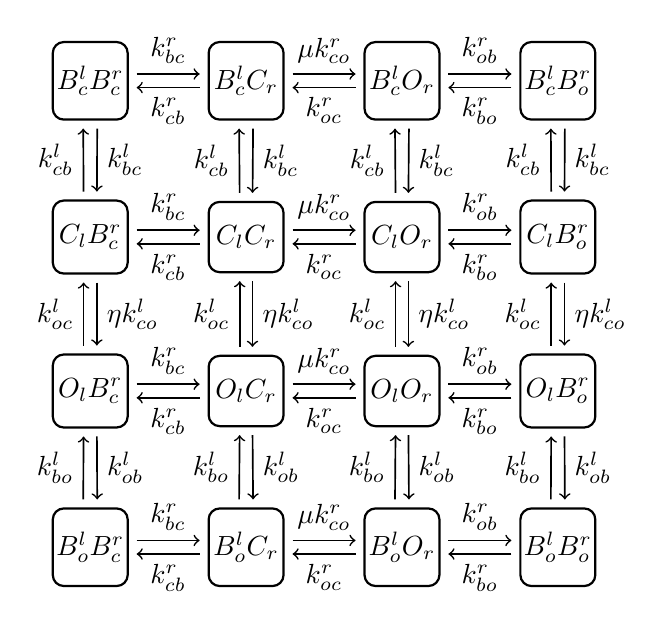
\begin{tikzpicture}[
   font=\sffamily,
   every matrix/.style={ampersand replacement=\&,column sep=1cm,row sep=1cm},
   state/.style={draw,thick,rounded corners,inner sep=.3cm},
   to/.style={->,semithick,shorten >=0.1cm,shorten <=0.1cm},
   Q/.style={->,semithick,sloped,pos=0.700000,shorten >=0.1cm,shorten <=0.1cm},  
   every node/.style={auto}]
\matrix{
\node[state] (B_{c}^{l}B_{c}^{r}) {\parbox{10pt}{\centerline{$B_{c}^{l}B_{c}^{r}$}}};\&\node[state] (B_{c}^{l}C_{r}) {\parbox{10pt}{\centerline{$B_{c}^{l}C_{r}$}}};\&\node[state] (B_{c}^{l}O_{r}) {\parbox{10pt}{\centerline{$B_{c}^{l}O_{r}$}}};\&\node[state] (B_{c}^{l}B_{o}^{r}) {\parbox{10pt}{\centerline{$B_{c}^{l}B_{o}^{r}$}}};\\
\node[state] (C_{l}B_{c}^{r}) {\parbox{10pt}{\centerline{$C_{l}B_{c}^{r}$}}};\&\node[state] (C_{l}C_{r}) {\parbox{10pt}{\centerline{$C_{l}C_{r}$}}};\&\node[state] (C_{l}O_{r}) {\parbox{10pt}{\centerline{$C_{l}O_{r}$}}};\&\node[state] (C_{l}B_{o}^{r}) {\parbox{10pt}{\centerline{$C_{l}B_{o}^{r}$}}};\\
\node[state] (O_{l}B_{c}^{r}) {\parbox{10pt}{\centerline{$O_{l}B_{c}^{r}$}}};\&\node[state] (O_{l}C_{r}) {\parbox{10pt}{\centerline{$O_{l}C_{r}$}}};\&\node[state] (O_{l}O_{r}) {\parbox{10pt}{\centerline{$O_{l}O_{r}$}}};\&\node[state] (O_{l}B_{o}^{r}) {\parbox{10pt}{\centerline{$O_{l}B_{o}^{r}$}}};\\
\node[state] (B_{o}^{l}B_{c}^{r}) {\parbox{10pt}{\centerline{$B_{o}^{l}B_{c}^{r}$}}};\&\node[state] (B_{o}^{l}C_{r}) {\parbox{10pt}{\centerline{$B_{o}^{l}C_{r}$}}};\&\node[state] (B_{o}^{l}O_{r}) {\parbox{10pt}{\centerline{$B_{o}^{l}O_{r}$}}};\&\node[state] (B_{o}^{l}B_{o}^{r}) {\parbox{10pt}{\centerline{$B_{o}^{l}B_{o}^{r}$}}};\\
};
\draw[to]  (B_{c}^{l}B_{c}^{r}.10) to node {$k_{bc}^{r}$} (B_{c}^{l}C_{r}.170);
\draw[to]  (B_{c}^{l}B_{c}^{r}.280) to node {$k_{bc}^{l}$} (C_{l}B_{c}^{r}.80);
\draw[to]  (B_{c}^{l}C_{r}.190) to node {$k_{cb}^{r}$} (B_{c}^{l}B_{c}^{r}.350);
\draw[to]  (B_{c}^{l}C_{r}.10) to node {$\mu k_{co}^{r}$} (B_{c}^{l}O_{r}.170);
\draw[to]  (B_{c}^{l}C_{r}.280) to node {$k_{bc}^{l}$} (C_{l}C_{r}.80);
\draw[to]  (B_{c}^{l}O_{r}.190) to node {$k_{oc}^{r}$} (B_{c}^{l}C_{r}.350);
\draw[to]  (B_{c}^{l}O_{r}.10) to node {$k_{ob}^{r}$} (B_{c}^{l}B_{o}^{r}.170);
\draw[to]  (B_{c}^{l}O_{r}.280) to node {$k_{bc}^{l}$} (C_{l}O_{r}.80);
\draw[to]  (B_{c}^{l}B_{o}^{r}.190) to node {$k_{bo}^{r}$} (B_{c}^{l}O_{r}.350);
\draw[to]  (B_{c}^{l}B_{o}^{r}.280) to node {$k_{bc}^{l}$} (C_{l}B_{o}^{r}.80);
\draw[to]  (C_{l}B_{c}^{r}.100) to node {$k_{cb}^{l}$} (B_{c}^{l}B_{c}^{r}.260);
\draw[to]  (C_{l}B_{c}^{r}.10) to node {$k_{bc}^{r}$} (C_{l}C_{r}.170);
\draw[to]  (C_{l}B_{c}^{r}.280) to node {$\eta k_{co}^{l}$} (O_{l}B_{c}^{r}.80);
\draw[to]  (C_{l}C_{r}.100) to node {$k_{cb}^{l}$} (B_{c}^{l}C_{r}.260);
\draw[to]  (C_{l}C_{r}.190) to node {$k_{cb}^{r}$} (C_{l}B_{c}^{r}.350);
\draw[to]  (C_{l}C_{r}.10) to node {$\mu k_{co}^{r}$} (C_{l}O_{r}.170);
\draw[to]  (C_{l}C_{r}.280) to node {$\eta k_{co}^{l}$} (O_{l}C_{r}.80);
\draw[to]  (C_{l}O_{r}.100) to node {$k_{cb}^{l}$} (B_{c}^{l}O_{r}.260);
\draw[to]  (C_{l}O_{r}.190) to node {$k_{oc}^{r}$} (C_{l}C_{r}.350);
\draw[to]  (C_{l}O_{r}.10) to node {$k_{ob}^{r}$} (C_{l}B_{o}^{r}.170);
\draw[to]  (C_{l}O_{r}.280) to node {$\eta k_{co}^{l}$} (O_{l}O_{r}.80);
\draw[to]  (C_{l}B_{o}^{r}.100) to node {$k_{cb}^{l}$} (B_{c}^{l}B_{o}^{r}.260);
\draw[to]  (C_{l}B_{o}^{r}.190) to node {$k_{bo}^{r}$} (C_{l}O_{r}.350);
\draw[to]  (C_{l}B_{o}^{r}.280) to node {$\eta k_{co}^{l}$} (O_{l}B_{o}^{r}.80);
\draw[to]  (O_{l}B_{c}^{r}.100) to node {$k_{oc}^{l}$} (C_{l}B_{c}^{r}.260);
\draw[to]  (O_{l}B_{c}^{r}.10) to node {$k_{bc}^{r}$} (O_{l}C_{r}.170);
\draw[to]  (O_{l}B_{c}^{r}.280) to node {$k_{ob}^{l}$} (B_{o}^{l}B_{c}^{r}.80);
\draw[to]  (O_{l}C_{r}.100) to node {$k_{oc}^{l}$} (C_{l}C_{r}.260);
\draw[to]  (O_{l}C_{r}.190) to node {$k_{cb}^{r}$} (O_{l}B_{c}^{r}.350);
\draw[to]  (O_{l}C_{r}.10) to node {$\mu k_{co}^{r}$} (O_{l}O_{r}.170);
\draw[to]  (O_{l}C_{r}.280) to node {$k_{ob}^{l}$} (B_{o}^{l}C_{r}.80);
\draw[to]  (O_{l}O_{r}.100) to node {$k_{oc}^{l}$} (C_{l}O_{r}.260);
\draw[to]  (O_{l}O_{r}.190) to node {$k_{oc}^{r}$} (O_{l}C_{r}.350);
\draw[to]  (O_{l}O_{r}.10) to node {$k_{ob}^{r}$} (O_{l}B_{o}^{r}.170);
\draw[to]  (O_{l}O_{r}.280) to node {$k_{ob}^{l}$} (B_{o}^{l}O_{r}.80);
\draw[to]  (O_{l}B_{o}^{r}.100) to node {$k_{oc}^{l}$} (C_{l}B_{o}^{r}.260);
\draw[to]  (O_{l}B_{o}^{r}.190) to node {$k_{bo}^{r}$} (O_{l}O_{r}.350);
\draw[to]  (O_{l}B_{o}^{r}.280) to node {$k_{ob}^{l}$} (B_{o}^{l}B_{o}^{r}.80);
\draw[to]  (B_{o}^{l}B_{c}^{r}.100) to node {$k_{bo}^{l}$} (O_{l}B_{c}^{r}.260);
\draw[to]  (B_{o}^{l}B_{c}^{r}.10) to node {$k_{bc}^{r}$} (B_{o}^{l}C_{r}.170);
\draw[to]  (B_{o}^{l}C_{r}.100) to node {$k_{bo}^{l}$} (O_{l}C_{r}.260);
\draw[to]  (B_{o}^{l}C_{r}.190) to node {$k_{cb}^{r}$} (B_{o}^{l}B_{c}^{r}.350);
\draw[to]  (B_{o}^{l}C_{r}.10) to node {$\mu k_{co}^{r}$} (B_{o}^{l}O_{r}.170);
\draw[to]  (B_{o}^{l}O_{r}.100) to node {$k_{bo}^{l}$} (O_{l}O_{r}.260);
\draw[to]  (B_{o}^{l}O_{r}.190) to node {$k_{oc}^{r}$} (B_{o}^{l}C_{r}.350);
\draw[to]  (B_{o}^{l}O_{r}.10) to node {$k_{ob}^{r}$} (B_{o}^{l}B_{o}^{r}.170);
\draw[to]  (B_{o}^{l}B_{o}^{r}.100) to node {$k_{bo}^{l}$} (O_{l}B_{o}^{r}.260);
\draw[to]  (B_{o}^{l}B_{o}^{r}.190) to node {$k_{bo}^{r}$} (B_{o}^{l}O_{r}.350);
\end{tikzpicture}
\end{center}
\caption{The Markov model represented in Figure \ref{eq:m_rl} extended to
account for blockers for the LCC and the RyR.}%
\label{Eq:m_rl2}%
\end{figure}
This model consists of 16 separate states given by
\begin{equation}%
\begin{tabular}
[c]{cccc}
$B_{c}^{l}B_{c}^{r}$ & $B_{c}^{l}C_{r}$ & $B_{c}^{l}O_{r}$ & $B_{c}^{l}B_{o}^{r}$\\
$C_{l}B_{c}^{r}$ & $C_{l}C_{r}$ & $C_{l}O_{r}$ & $C_{l}B_{o}^{r}$\\
$O_{l}B_{c}^{r}$ & $O_{l}C_{r}$ & $O_{l}O_{r}$ & $O_{l}B_{o}^{r}$\\
$B_{o}^{l} B_{c}^{r}$ & $B_{o}^{l}C_{r}$ & $B_{o}^{l}O_{r}$ &$B_{o}^{l}B_{o}^{r}$
\end{tabular}
\ \ \
\end{equation}
and the combined LCC and RyR drug is fully specified by
\begin{equation}
k_{cb}^{r},k_{bc}^{r},k_{bo}^{r},k_{ob}^{r},k_{cb}^{l},k_{bc}^{l}, k_{bo}^{l}, \text{ and }k_{ob}^{l}.
\end{equation}






\section[Probability density functions;16 state model]{Probability density functions associated with the 16-state model}

As mentioned in Chapter \ref{general} (see page \pageref{general}), it is convenient to use a more compact notation to represent the system of partial differential equations governing the probability density functions when the Markov model consists of numerous states. By using the notation introduced in Chapter \ref{general} , we can write the probability density system associated with the Markov model in Figure \ref{Eq:m_rl2} in the form
\begin{equation}
\frac{\partial\rho_{ij}}{\partial t}+\frac{\partial}{\partial x}\left(
a_{ij}^{x}\rho_{ij}\right)  +\frac{\partial}{\partial y}\left(  a_{ij}^{y}%
\rho_{ij}\right)  =R_{ij}, \label{pdf16}%
\end{equation}
where%
\begin{align*}
R_{ij}  & =K_{i,j+1}^{i,j}\rho_{i,j+1}+K_{i+1,j}^{i,j}\rho_{i+1,j}%
+K_{i,j-1}^{i,j}\rho_{i,j-1}+K_{i-1,j}^{i,j}\rho_{i-1,j}\\
& -\left(  K_{i,j}^{i,j+1}+K_{i,j}^{i+1,j}+K_{i,j}^{i,j-1}+K_{i,j}%
^{i-1,j}\right)  \rho_{i,j}.
\end{align*}
 The flux terms are given by%
\begin{align*}
a_{ij}^{x} &  =\gamma^{r}_{i}v_{r}\left(  y-x\right)  +v_{d}\left(
c_{0}-x\right) -\gamma^{l}_{j}J_{l} ,\\
a_{ij}^{y} &  =\gamma^{r}_{i}v_{r}\left(  x-y\right)  +v_{s}\left(
c_{1}-y\right)  ,
\end{align*}
where $\gamma^{r}_{i}=1$ when the RyR state is open and
$\gamma^{r}_{i}=0$ when the RyR state is closed and similarly for $\gamma^{l}$ and the LCC.

%Here we have formulated the system
%(\ref{Eq:m_rl2}) on the form (\ref{ninestates}) with an obvious extension from a nine state to
%a 16 state model. In the two dimensional numbering we 
%have $\gamma_{ij}=\gamma^l_i \gamma^r_j$ where 
%$\gamma^l_1=\gamma^l_3=\gamma^l_4=0$ and $\gamma^l_2=1$. And similarly,
%$\gamma^r_1=\gamma^r_2=\gamma^r_4=0$ and $\gamma^r_3=1$.

\section[RyR mutations]{RyR mutations under a varying transmembrane potential}

In this section, we assume that a mutation affects the RyR such that the
mutation severity index is increased. This problem has been discussed several times above, but here
we also need to take into account that the value of the transmembrane potential may change. In our computations, we use $\mu=3$ and
we try to repair the effect of the mutation by adding a closed state blocker
to the Markov model of the RyR channel. 
The Markov model is shown in Figure \ref{m_ryr_c}.%
\begin{figure}[ptb]
\begin{center}
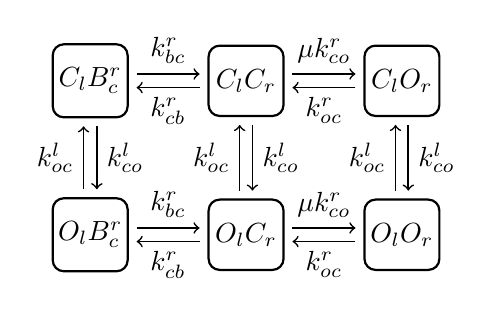
\begin{tikzpicture}[
   font=\sffamily,
   every matrix/.style={ampersand replacement=\&,column sep=1cm,row sep=1cm},
   state/.style={draw,thick,rounded corners,inner sep=.3cm},
   to/.style={->,semithick,shorten >=0.1cm,shorten <=0.1cm},
   Q/.style={->,semithick,sloped,pos=0.700000,shorten >=0.1cm,shorten <=0.1cm},  
   every node/.style={auto}]
\matrix{
\node[state] (C_{l}B_{c}^{r}) {\parbox{10pt}{\centerline{$C_{l}B_{c}^{r}$}}};\&\node[state] (C_{l}C_{r}) {\parbox{10pt}{\centerline{$C_{l}C_{r}$}}};\&\node[state] (C_{l}O_{r}) {\parbox{10pt}{\centerline{$C_{l}O_{r}$}}};\\
\node[state] (O_{l}B_{c}^{r}) {\parbox{10pt}{\centerline{$O_{l}B_{c}^{r}$}}};\&\node[state] (O_{l}C_{r}) {\parbox{10pt}{\centerline{$O_{l}C_{r}$}}};\&\node[state] (O_{l}O_{r}) {\parbox{10pt}{\centerline{$O_{l}O_{r}$}}};\\
};
\draw[to]  (C_{l}B_{c}^{r}.10) to node {$k_{bc}^{r}$} (C_{l}C_{r}.170);
\draw[to]  (C_{l}B_{c}^{r}.280) to node {$k_{co}^{l}$} (O_{l}B_{c}^{r}.80);
\draw[to]  (C_{l}C_{r}.190) to node {$k_{cb}^{r}$} (C_{l}B_{c}^{r}.350);
\draw[to]  (C_{l}C_{r}.10) to node {$\mu k_{co}^{r}$} (C_{l}O_{r}.170);
\draw[to]  (C_{l}C_{r}.280) to node {$k_{co}^{l}$} (O_{l}C_{r}.80);
\draw[to]  (C_{l}O_{r}.190) to node {$k_{oc}^{r}$} (C_{l}C_{r}.350);
\draw[to]  (C_{l}O_{r}.280) to node {$k_{co}^{l}$} (O_{l}O_{r}.80);
\draw[to]  (O_{l}B_{c}^{r}.100) to node {$k_{oc}^{l}$} (C_{l}B_{c}^{r}.260);
\draw[to]  (O_{l}B_{c}^{r}.10) to node {$k_{bc}^{r}$} (O_{l}C_{r}.170);
\draw[to]  (O_{l}C_{r}.100) to node {$k_{oc}^{l}$} (C_{l}C_{r}.260);
\draw[to]  (O_{l}C_{r}.190) to node {$k_{cb}^{r}$} (O_{l}B_{c}^{r}.350);
\draw[to]  (O_{l}C_{r}.10) to node {$\mu k_{co}^{r}$} (O_{l}O_{r}.170);
\draw[to]  (O_{l}O_{r}.100) to node {$k_{oc}^{l}$} (C_{l}O_{r}.260);
\draw[to]  (O_{l}O_{r}.190) to node {$k_{oc}^{r}$} (O_{l}C_{r}.350);
\end{tikzpicture}
\end{center}
\caption{The Markov model represented in Figure \ref{eq:m_rl} extended to 
include an RyR mutation and a closed state blocker for the RyR.}%
\label{m_ryr_c}%
\end{figure}

The closed state drug applied to the RyR channel is represented by the two
parameters $k_{cb}^{r}$ and $k_{bc}^{r}.$ We have seen above that for closed
state blockers of the RyR it is reasonable to define%
\[
k_{cb}^{r}=\left(  \mu-1\right)  k_{bc}^{r},%
\]
where the value of $k_{bc}^{r}$ remains to be decided. 

\subsection{Theoretical closed state blocker repairs the open probabilities of the RyR CO-mutation}

Numerical results using the closed state drug shown in Figure \ref{m_ryr_c} are given 
in Figure \ref{cicr/ryr_cbI.pdf}. Note that we aim to repair the probability of being in the open state and are not interested in whether the channel is in a blocked state or in a closed state. The probability of being in a closed or blocked state is therefore 
added in the graphs. We observe from the graphs that 
the mutant channel is completely repaired by the closed state blocker.

In Figure \ref{cicr/ryr_cbXY.pdf}, we show the development of the expected concentrations of the dyad ($x$) and the junctional sarcoplasmic reticulum  (JSR) ($y$) and observe that 
the expected concentrations are repaired by a sufficiently strong version of the blocker associated with the closed state of the RyR channel.


\fig{cicr/ryr_cbI.pdf}{Total probabilities based on the model for the probability density functions associated with the Markov model
in Figure \ref{m_ryr_c}. A closed state blocker is applied, the mutation severity index is $\mu=3$, and the transmembrane potential is $V=0$ mV.
The plots show the total probability of being in the state OO, (OC+OB), CO, or (CC+CB) as a function of 
$k^r_{bc}$. In the upper left plot, the total probability of being in the OO state is higher for the mutant than for the wild type. This is repaired by the closed 
state drug. Similar results are shown for the other states. }

\fig{cicr/ryr_cbXY.pdf}{Based on the probability density functions of the states OO, (OC+OB), CO, and (CC+CB), we can compute the
expected concentrations of the dyad ($x$) and the JSR ($y$). The wild type is denoted by $\circ$ and the RyR mutation index $\mu$ increases from one to three along the solid line. In the dashed line, we keep $\mu=3$ and increase the value of $k^r_{bc}$ from 0 $\rm{ms^{-1}}$ to 100 $\rm{ms^{-1}}$. We observe that as $k^r_{bc}$  increases, the 
expected concentrations are completely repaired. The experiment is carried out for the case of $V=0$ mV.}


\subsection{The open state blocker does not work as well as the closed state blocker for CO-mutations in RyR}
%\K{zzz Kanskje denne underseksjonen heller burde st\r{a} under forrige seksjon
%siden den handler om RyR-mutasjoner?}
%\{I moved it}

In Table \ref{ryr_ob},  we report on the performance of the open and closed state blockers for the RyR mutation. Recall that the probability $\pi_{oo}$, the expected dyad concentration ($E^x_{oo}$), and the expected JSR concentration ($E^y_{oo}$) are defined on page \pageref{statistics}.  The closed blocker clearly is best suited to repair this mutation.





\begin{table}  \begin{center}
\begin{tabular}{|c|r|r|r|r|} \hline
&WT & MT & Optimal closed blocker & Optimal open blocker \\ \hline
$10^3\times\pi_{oo}$&2.75 & 5.11 & 2.74 & 0.81 \\ \hline
$E^x_{oo}$&51.87 & 45.62 & 51.92 & 52.46 \\ \hline
$E^y_{oo}$&751.76 & 544.30 & 751.99 & 713.89 \\ \hline
\end{tabular} \end{center}
\caption{Properties of the probability density function ($\rho_{oo}$) of being in the state OO with $\mu=3$ (and  $\eta=1$). The closed state blocker works fine in the sense that it is well suited for repairing a CO-mutation of the RyR. 
The  open state blocker is unable to completely repair the effect of the mutation. The open state blocker is found using Matlab's {\it Fminsearch},
with a cost function defined to minimize the difference between the wild type and the mutation when the drug is applied.
In this table, WT and MT mean wild type and mutant, respectively, and  $V=0$ mV is used in the simulations.
%{\bf xxx Glenn:Something is wrong since the integral of $\rho_{oo}$ larger than one.}
%\G{These were scaled by 1000, now noted in the table.}
} \label{ryr_ob}
\end{table}



%{\bf: Glenn:} Can you make a plot of the type given in the upper left corner of Figure  \ref{cicr/ryr_cbXY.pdf}, Where you %have one panel for all the voltages:
%−80, −60, −40, −20, 0, 20 mV? We should comment on that this holds for varying voltage. 

\section[LCC mutations]{LCC mutations under a varying transmembrane potential}

Next, we address the problem of defining a theoretical drug for LCC
mutations. We consider closed state LCC blockers of the form 
given in Figure \ref{m_lcc_c} and open state blockers of the form
given in Figure \ref{m_lcc_o}.%

\begin{figure}[ptb]
\begin{center}
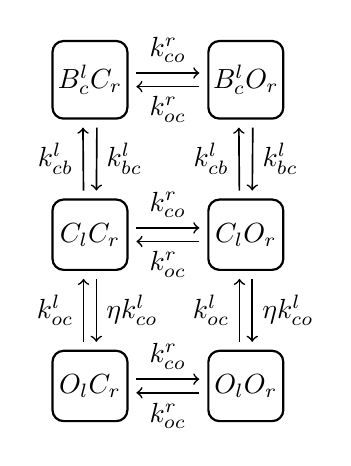
\begin{tikzpicture}[
   font=\sffamily,
   every matrix/.style={ampersand replacement=\&,column sep=1cm,row sep=1cm},
   state/.style={draw,thick,rounded corners,inner sep=.3cm},
   to/.style={->,semithick,shorten >=0.1cm,shorten <=0.1cm},
   Q/.style={->,semithick,sloped,pos=0.700000,shorten >=0.1cm,shorten <=0.1cm},  
   every node/.style={auto}]
\matrix{
\node[state] (B_{c}^{l}C_{r}) {\parbox{10pt}{\centerline{$B_{c}^{l}C_{r}$}}};\&\node[state] (B_{c}^{l}O_{r}) {\parbox{10pt}{\centerline{$B_{c}^{l}O_{r}$}}};\\
\node[state] (C_{l}C_{r}) {\parbox{10pt}{\centerline{$C_{l}C_{r}$}}};\&\node[state] (C_{l}O_{r}) {\parbox{10pt}{\centerline{$C_{l}O_{r}$}}};\\
\node[state] (O_{l}C_{r}) {\parbox{10pt}{\centerline{$O_{l}C_{r}$}}};\&\node[state] (O_{l}O_{r}) {\parbox{10pt}{\centerline{$O_{l}O_{r}$}}};\\
};
\draw[to]  (B_{c}^{l}C_{r}.10) to node {$k_{co}^{r}$} (B_{c}^{l}O_{r}.170);
\draw[to]  (B_{c}^{l}C_{r}.280) to node {$k_{bc}^{l}$} (C_{l}C_{r}.80);
\draw[to]  (B_{c}^{l}O_{r}.190) to node {$k_{oc}^{r}$} (B_{c}^{l}C_{r}.350);
\draw[to]  (B_{c}^{l}O_{r}.280) to node {$k_{bc}^{l}$} (C_{l}O_{r}.80);
\draw[to]  (C_{l}C_{r}.100) to node {$k_{cb}^{l}$} (B_{c}^{l}C_{r}.260);
\draw[to]  (C_{l}C_{r}.10) to node {$k_{co}^{r}$} (C_{l}O_{r}.170);
\draw[to]  (C_{l}C_{r}.280) to node {$\eta k_{co}^{l}$} (O_{l}C_{r}.80);
\draw[to]  (C_{l}O_{r}.100) to node {$k_{cb}^{l}$} (B_{c}^{l}O_{r}.260);
\draw[to]  (C_{l}O_{r}.190) to node {$k_{oc}^{r}$} (C_{l}C_{r}.350);
\draw[to]  (C_{l}O_{r}.280) to node {$\eta k_{co}^{l}$} (O_{l}O_{r}.80);
\draw[to]  (O_{l}C_{r}.100) to node {$k_{oc}^{l}$} (C_{l}C_{r}.260);
\draw[to]  (O_{l}C_{r}.10) to node {$k_{co}^{r}$} (O_{l}O_{r}.170);
\draw[to]  (O_{l}O_{r}.100) to node {$k_{oc}^{l}$} (C_{l}O_{r}.260);
\draw[to]  (O_{l}O_{r}.190) to node {$k_{oc}^{r}$} (O_{l}C_{r}.350);
\end{tikzpicture}
\end{center}
\caption{The Markov model represented in Figure \ref{eq:m_rl} extended to 
include an LCC mutation and a closed state blocker for the LCC.}%
\label{m_lcc_c}%
\end{figure}

\begin{figure}[ptb]
\begin{center}
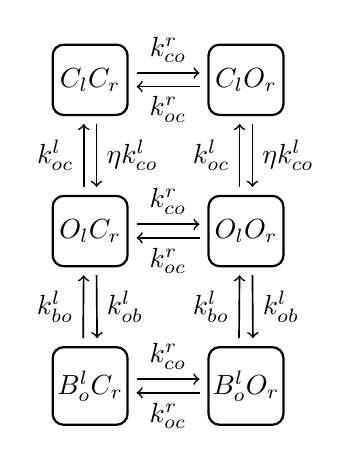
\begin{tikzpicture}[
   font=\sffamily,
   every matrix/.style={ampersand replacement=\&,column sep=1cm,row sep=1cm},
   state/.style={draw,thick,rounded corners,inner sep=.3cm},
   to/.style={->,semithick,shorten >=0.1cm,shorten <=0.1cm},
   Q/.style={->,semithick,sloped,pos=0.700000,shorten >=0.1cm,shorten <=0.1cm},  
   every node/.style={auto}]
\matrix{
\node[state] (C_{l}C_{r}) {\parbox{10pt}{\centerline{$C_{l}C_{r}$}}};\&\node[state] (C_{l}O_{r}) {\parbox{10pt}{\centerline{$C_{l}O_{r}$}}};\\
\node[state] (O_{l}C_{r}) {\parbox{10pt}{\centerline{$O_{l}C_{r}$}}};\&\node[state] (O_{l}O_{r}) {\parbox{10pt}{\centerline{$O_{l}O_{r}$}}};\\
\node[state] (B_{o}^{l}C_{r}) {\parbox{10pt}{\centerline{$B_{o}^{l}C_{r}$}}};\&\node[state] (B_{o}^{l}O_{r}) {\parbox{10pt}{\centerline{$B_{o}^{l}O_{r}$}}};\\
};
\draw[to]  (C_{l}C_{r}.10) to node {$k_{co}^{r}$} (C_{l}O_{r}.170);
\draw[to]  (C_{l}C_{r}.280) to node {$\eta k_{co}^{l}$} (O_{l}C_{r}.80);
\draw[to]  (C_{l}O_{r}.190) to node {$k_{oc}^{r}$} (C_{l}C_{r}.350);
\draw[to]  (C_{l}O_{r}.280) to node {$\eta k_{co}^{l}$} (O_{l}O_{r}.80);
\draw[to]  (O_{l}C_{r}.100) to node {$k_{oc}^{l}$} (C_{l}C_{r}.260);
\draw[to]  (O_{l}C_{r}.10) to node {$k_{co}^{r}$} (O_{l}O_{r}.170);
\draw[to]  (O_{l}C_{r}.280) to node {$k_{ob}^{l}$} (B_{o}^{l}C_{r}.80);
\draw[to]  (O_{l}O_{r}.100) to node {$k_{oc}^{l}$} (C_{l}O_{r}.260);
\draw[to]  (O_{l}O_{r}.190) to node {$k_{oc}^{r}$} (O_{l}C_{r}.350);
\draw[to]  (O_{l}O_{r}.280) to node {$k_{ob}^{l}$} (B_{o}^{l}O_{r}.80);
\draw[to]  (B_{o}^{l}C_{r}.100) to node {$k_{bo}^{l}$} (O_{l}C_{r}.260);
\draw[to]  (B_{o}^{l}C_{r}.10) to node {$k_{co}^{r}$} (B_{o}^{l}O_{r}.170);
\draw[to]  (B_{o}^{l}O_{r}.100) to node {$k_{bo}^{l}$} (O_{l}O_{r}.260);
\draw[to]  (B_{o}^{l}O_{r}.190) to node {$k_{oc}^{r}$} (B_{o}^{l}C_{r}.350);
\end{tikzpicture}
\end{center}
\caption{The Markov model represented in Figure \ref{eq:m_rl} extended to 
include an LCC mutation and an open state blocker for the LCC.}%
\label{m_lcc_o}%
\end{figure}

For the closed state blockers, we need to determine the two parameters
$k_{bc}^{l}$ and $k_{cb}^{l}$ and for the open state blockers we must determine
$k_{bo}^{l}$ and $k_{ob}^{l}.$ For the closed state blockers we define%
\[
k_{cb}^{l}=\left(  \eta-1\right)  k_{bc}^{l}%
\]
and we consider various values of $k_{bc}^{l}.$  

%For the open state blocker we use (as above)
%straightforward optimization to minimize the norm xxx. This gives
%\[
%k_{ob}^{l}=xxx\text{ and }k_{bo}^{l}=xxx.
%\]

\subsection{The closed state blocker repairs the open probabilities of the LCC mutant}

The results of applying the theoretical closed state blocker associated with the closed state  (see Figure \ref{m_lcc_c}) of the LCC are given in Figures
\ref{cicr/lcc_cbI.pdf} to \ref{cicr/lcc_cb_V.pdf}. In the first figure, we show how the closed state blocker repairs the total probabilities and in the second figure we consider the expected concentrations. In Figure  \ref{cicr/lcc_cb_V.pdf}, we show how the expected concentrations are repaired for six values of the transmembrane potential.


\fig{cicr/lcc_cbI.pdf}{Total probabilities based on the model for the probability density functions associated with the Markov model
in Figure \ref{m_lcc_c}, where an LCC-type closed state blocker is included. The LCC mutation severity index is $\eta=3$ and the transmembrane potential is $V=0$ mV.
The plots show the total probability of being in the state OO, OC, (CO+BO), or (CC+BC) as a function of 
$k^l_{bc}$. In the upper left plot, the total probability of being in the OO state is higher for the mutant than for the wild type. This is repaired by the closed state drug. Similar results are shown for the other states.}

\fig{cicr/lcc_cbXY.pdf}{Using the probability density functions of the states OO, OC, (CO+BO), and (CC+BC), we compute the
expected concentrations of the dyad ($x$) and the JSR ($y$). The wild type is denoted by $\circ$ and the LCC mutation index $\eta$ increases from one to three along the solid line. In the dashed line, we keep $\eta=3$ and increase the value of $k^l_{bc}$ from 0 $\rm{ms^{-1}}$ to 100 $\rm{ms^{-1}}$. We observe that as $k^l_{bc}$ increases, the 
expected concentrations are completely repaired. The simulations are performed using $V=0$ mV.}

\fig{cicr/lcc_cb_V.pdf}{ The expected  concentration of the dyad ($x$) and the JSR ($y$) for the OO state for the transmembrane potential
changing from -80 mV to 20 mV. The wild type is denoted by $\circ$ and the LCC mutation index $\eta$ increases from one to three along the solid line. In the dashed line, we keep $\eta=3$ and increase the value of $k^l_{bc}$ from 0 $\rm{ms^{-1}}$ to 100 $\rm{ms^{-1}}$.  In all cases, the closed state blocker repairs the effect of the mutation.
%{\bf xxx Glenn: check that text here is consistent with simulation. Remove if ok.} 
}

%{\bf: Glenn:} Can you make a plot of the type given in the upper left corner of Figure  \ref{cicr/lcc_cbXY.pdf}, Where you have one panel for all the voltages:
%−80, −60, −40, −20, 0, 20 mV? We should comment on that this holds for varying voltage. 

%\subsection{The closed state blocker for RyR does not repair the open probabilities of the LCC mutant}

%Here we check if it is possible to use a closed state blocker on RyR to repair the open probabilities of the LCC mutant. The last column of Table \ref{cross} shows the performanance in terms of restoring $\rho_{oo}$.

%\begin{table}  \begin{center}
%\begin{tabular}{|l|r|r|r|r|} \hline
%&WT & MT & $k^l_{cb}$ & $k^r_{cb}$ \\ \hline
%$\int \rho_{oo}$ &2.75 & 8.59 & 2.75 & 2.44 \\ \hline
%$\int x \rho_{oo}$&51.87 & 46.55 & 51.87 & 49.79 \\ \hline
%$\int y \rho_{oo}$ &751.76 & 580.88 & 751.77 & 657.87 \\ \hline
%\end{tabular} \end{center}
%\caption{Properties of $\rho_{oo}$, $\eta=3$ (and  $\mu=1$). Closed blocker on LCC works fine as seen before. Closed blocker on RyR not so much.The RyR blocker has been found using fminsearch. Cost function tried to minimize error in the overall expected values (overall meaning sum over all pdfs), mostly weighted on $x$ since this is the one that comunicates with the contractile units: $\sqrt{((x-x_{wt})/x_{wt})^2 + 0.1*((y-y_{wt})/y_{wt})^2}$
%} \label{cross}
%\end{table}





\chapter{A prototypical model of an ion channel}
\label{prototype}

So far we have been concerned with calcium-induced calcium release (CICR) as
illustrated in Figure \ref{geomCa_V} (page \pageref{geomCa_V}). To
study CICR, we started by studying the development of the concentration of
calcium ions in the dyad and kept everything else constant. The interesting
part was then to see how the release mechanism of the ryanodine receptor RyR changes 
the dynamics of the dyad concentration. In particular, we were interested in RyR 
mutations and their theoretical effect on the dyad concentration through changes in the
open probability of the RyR channel. We saw how theoretical blockers could be
defined in order to repair the effect of the mutations, in the sense that we
were able to restore essential properties of the process. We also introduced the
effect of allowing the concentration of the junctional sarcoplasmic reticulum 
 to change and we studied how the overall processes were affected by introducing 
 the transmembrane potential and allowing the L-type calcium channel (LCC) to open and close. 

Now we leave the RyR and Markov
models based on concentrations of calcium ions and focus on
voltage-gated channels. We touched upon this topic earlier, since the LCC
is voltage gated, but now we will dynamically update the voltage and focus
solely on how voltage develops and how it affects the transitions of the
Markov model.

We will start by studying a very simple channel to explain
the basics steps as carefully as possible. This channel does not have a name and
probably does not exist in nature, but it provides a good example to
get a handle on the steps involved in understanding much more complex (and more
realistic) ion channels. 
%In later chapters we will focus on both Sodium and Potassium channels and study theoretical drugs for these channels.

In the study of CICR, we examined what was going on in a very small part of the 
cell based on the tacit assumption that if we can repair what is going on in 
every tiny part of the cell, we will probably also do a decent job in repairing all of the cell. We will follow the same strategy in studying voltage-gated channels: We will study a single channel and see how mutations may affect the 
function of the channel and thereby how the transmembrane potential is changed. Again, we will derive 
theoretical drugs and see how they should be defined in order to repair the effect of the mutations. However, the assumption that small domains can be studied independently is less reliable for voltage-gated channels than for 
the CICR process in the vicinity of the dyad. The reason for this is that electrical diffusion waves travel much faster than concentration waves. %Therefore we will conclude our analysis of voltage-gated ion channels by adding many of them together and study the whole cell effect of the theoretical drugs we propose. This will be done in Chapter \ref{ap}, but first we will spend some time studying single channels.

\section[Stochastic model]{Stochastic model of the transmembrane potential}

The transmembrane potential is defined to be the difference between the
intracellular potential $v_{i}$ and the extracellular potential $v_{e}$:
\begin{equation}
v=v_{i}-v_{e}. \label{v0}
\end{equation}
Let us consider a membrane consisting of a leakage current with conductance
given by $g_{L}$ and an ion channel with conductance given by $g_{i}.$ The
transmembrane potential of such a membrane is governed by the
differential equation
\begin{equation}
Cv^{\prime}=-g_{L}\left(  v-V_{L}\right)  -g_{i}(v-V_{i}), \label{v1}
\end{equation}
where $C$ is the capacitance of the membrane, $V_{L}$ is the resting potential
of the leakage current, and $V_{i}$ is the resting potential of the ion
channel. In our computations, we will consider an example\footnote{Here, the choice of the parameter $V_i$ may seem a bit strange, but we will see below that it will lead to a very simple computational domain for the probability density functions.} 
with the parameters listed in Table \ref{11on10}.
\graytable{l}{
{|c|c|} \hline
$C$ &  $1$ $\mu\text{F/cm}^{2}$\\ \hline
$g_L$ & $1/10 \text{ mS/cm}^{2}$ \\ \hline
$V_L$ & $0\text{ mV}$ \\ \hline
$V_{i}$ & $11/10\text{ mV}$\\ \hline
}{ Values of the parameters used in the model \ref{v1}.\label{11on10}}
%\begin{align*}
%C  &  =1 \text{ } \mu\text{F/cm}^{2},\\
%g_{L}  &  =\frac{1}{10}\text{ mS/cm}^{2},\\
%V_{L}  &  =0\text{ mV,}\\
%V_{i}  &  =\frac{11}{10}\text{ mV.}
%\end{align*}
We assume that the ion channel can be either open (O), with $g_{i}=1$ mS/cm$^{2},$ or
closed (C), with $g_{i}=0$ mS/cm$^{2}$. The state of the stochastic ion channel is governed
by a Markov model of the form
\begin{equation}
C\underset{k_{co}}{\overset{k_{oc}}{\leftrightarrows}}O, \label{Markov_volt}
\end{equation}
where the reactions rates will be specified below. With these definitions, the
stochastic equation takes the form
\begin{equation}
v^{\prime}=-\frac{1}{10}v-\gamma\left(  v-\frac{11}{10}\right),  \label{v2}
\end{equation}
where $\gamma$ is zero (closed) or one (open) depending on the state of the Markov model (\ref{Markov_volt}).

\subsection{A numerical scheme}

We compute numerical solutions of the model (ref{v2}) using
the scheme
\begin{equation}
v_{n+1}=v_{n}-\Delta t\left(  \frac{1}{10}v_{n}+\gamma_{n}\left(  v_{n}
-\frac{11}{10}\right)  \right)  \label{vs},
\end{equation}
where $\Delta t$ denotes the time step and $\gamma_{n}$ takes on values
based on the state of the Markov model. Based on the Markov model, the value
of $\gamma_{n}$ is computed as described on page \pageref{numscheme}. We assume that
the time step (in ms) satisfies the condition
\begin{equation}
\Delta t<\frac{10}{11}. \label{vdt}
\end{equation}



\subsection{An invariant region}

We discussed above that it is useful to derive an invariant region for the
stochastic model since such a region can be used to define the computational
domain of the probability density equation. We claim that, under the condition
(ref{vdt}) for the time step, the solutions generated by 
scheme (ref{vs}) will always remain in the interval given by
\[
\Omega=(0,1),
\]
provided that the initial condition is in this region. To show that
$\Omega$ is an invariant region for solutions generated by scheme $\left(
\ref{vs}\right)  $, we write the scheme in the form
\[
v_{n+1}=H(v_{n},\gamma_{n}),
\]
where
\[
H(v,\gamma)=v-\Delta t\left(  \frac{1}{10}v+\gamma\left(  v-\frac{11}
{10}\right)  \right)  .
\]
Since
\[
\frac{\partial H(v,\gamma)}{\partial v}=1-\Delta t\left(  \frac{1}{10}
+\gamma\right)  >0
\]
because of (ref{vdt}) and
\[
\frac{\partial H(v,\gamma)}{\partial\gamma}=\Delta t\left(\frac{11}{10}-v\right)>0
\]
for any $v\in\Omega,$ we have
\[
v_{n+1}=H(v_{n},\gamma_{n})\leqslant H\left(  1,1\right)  =1
\]
and
\[
v_{n+1}=H(v_{n},\gamma_{n})\geqslant H(0,0)=0.
\]
So, by induction, we have  $v_{n}\in\Omega$  for all $n$.



\section[Probability density functions]{Probability density functions for the voltage-gated channel}

We can now follow exactly the same steps as in Section \ref{sec:pdf} (see page
\pageref{sec:pdf}) to derive a model of the probability density
functions of the open state and the closed state. The probability of the
channel being in the open state for voltages between $v$ and $v+\Delta v$ is
given by
\[
P_{o}\left\{  v<V(t)<v+\Delta v\right\}  =\int_{v}^{v+\Delta v}\rho_{o}(w,t)dw,
\]
where $\rho_{o}$ is the probability density function of the open state.
Similarly, we have
\[
P_{c}\left\{  v<V(t)<v+\Delta v\right\}  =\int_{v}^{v+\Delta v}\rho_{c}(w,t)dw
\]
where $\rho_{c}$ is the probability density function of the closed state. By
the arguments given in Section \ref{sec:pdf}, we find that the probability
density functions must be solutions of the system
\begin{align}
\frac{\partial\rho_{o}}{\partial t}+\frac{\partial}{\partial v}\left(
a_{o}\rho_{o}\right)   &  =k_{co}\rho_{c}-k_{oc}\rho_{o},\label{vpdf}\\
\frac{\partial\rho_{c}}{\partial t}+\frac{\partial}{\partial v}\left(
a_{c}\rho_{c}\right)   &  =k_{oc}\rho_{o}-k_{co}\rho_{c},\nonumber
\end{align}
where the flux terms are given by
\begin{align}
a_{o} &  =-g_{L}\left(  v-V_{L}\right)  -(v-V_{i})=\frac{11}{10}\left(
1-v\right)  ,\label{vflux}\\
a_{c} &  =-g_{L}\left(  v-V_{L}\right)  =-\frac{1}{10}v\nonumber
\end{align}
%\K{zzz Skal man egentlig dele p\r{a}  C i uttrykkene for $a_o$ og $a_c$ eller blir C-en bakt inn i ligningen p\r{a}  en annen m\r{a}te?}
%\A{In principle, yes, but since C=1, we do nothing (except that we changes units)}



As usual, the boundary conditions are set up to avoid a probability leak
across the boundary. Hence we need the  fluxes $a_{o}\rho_{o}$ and
$a_{c}\rho_{c}$ to be zero for $v=0$ and $v=1.$ Note that $a_{o}
(1)=a_{c}(0)=0;$ so we require $\rho_{o}(0)=0$ and $\rho_{c}(1)=0.$ In
the numerical simulations presented below, we use the scheme described in
Section \ref{npdf}. Stationary solutions of the numerical scheme are computed
as described on page \pageref{accuracy}.


\section{Analytical solution of the stationary case}

We showed in Section \ref{sec:analytical} how an analytical solution can be derived
for a stationary system of the form (ref{vpdf}) Here we
shall repeat this derivation for a voltage-gated channel. For simplicity we
shall consider a channel where the reaction scheme of the Markov model is
independent of the voltage; we choose
\[
k_{oc}=1\text{ ms}^{-1}\text{ and }k_{co}=\mu\text{ ms}^{-1}.
\]
So, we will again focus on CO-mutations.
Here $\mu$, referred to as the mutation severity index,
 will be specified in the computations below.  In all computations, $\mu=1$ will be 
 referred to as the wild type case. Increased values of
$k_{co}$ will increase the open probability of the ion channel in $\left(
\ref{v1}\right)  $ and therefore bring the transmembrane potential closer to
the maximum  value (given by $V_{+}=1$ mV). 

The first step in the derivation of the analytical solution is to observe that, in the
steady state, the sum of the equations of (ref{vpdf}) results
in the equation
\[
\frac{\partial}{\partial v}\left(  a_{o}\rho_{o}+a_{c}\rho_{c}\right)  =0.
\]
The second step is to observe that the boundary conditions imply that
\[
a_{o}\rho_{o}+a_{c}\rho_{c}=0.
\]
Therefore, for the present model, we find that
\[
\rho_{c}=-\frac{a_{o}}{a_{c}}\rho_{o}=\frac{11}{v}\left(  1-v\right)  \rho_{o}
\]
and, from (ref{vpdf}), we have
\[
\frac{\partial}{\partial v}\left(  a_{o}\rho_{o}\right)  =\mu\rho_{c}-\rho
_{o}=\left(  11\mu\frac{1-v}{v}-1\right)  \rho_{o}.
\]
By differentiation, we obtain
\[
a_{o}\frac{\partial}{\partial v}\rho_{o}=\left(  11\mu\frac{1-v}{v}
-1-\frac{\partial}{\partial v}a_{o}\right)  \rho_{o}
\]
and thus
\begin{equation}
\rho_{o}^{\prime}=a(v)\rho_{o}, \label{rho1}
\end{equation}
where
\[
a(v)=\left(  \frac{10\mu}{v}+\frac{1}{11(1-v)}\right)  .
\]
The solution of (ref{rho1}) is given by
\begin{equation}
\rho_{o}=c\frac{v^{10\mu}}{\left(  1-v\right)  ^{1/11}}\label{rho2}
\end{equation}
and then
\[
\rho_{c}=11 c \left(  1-v\right)  ^{10/11}v^{10\mu-1}.
\]
Here the constant $c$ must be chosen such that
\[
\int_{\Omega}\left(  \rho_{o}+\rho_{c}\right)  dv=1.
\]

It is interesting to note here that, even if both $\rho_o$ and $\rho_c$ depend heavily on the mutation severity 
index $\mu$, the relation between these functions is independent of $\mu$ since
\[ \frac{\rho_o}{\rho_c}=\frac{v}{11(1-v)}. \]

\section[Comparison of MCs and PDFs]{Comparison of Monte Carlo simulations and probability density functions}


In previous chapters we gave many examples showing that the probability density
functions faithfully represent the frequency distributions that can be
computed using Monte Carlo simulations. We will briefly show that this also
holds for the ion channel model considered here. In Figure \ref{V:mc_mut}, we compare the
open probability density function given by (ref{rho2}) and a
histogram computed using Monte Carlo simulations based on the numerical scheme
given by (ref{vs})  We observe again---and by now we are starting to get used to it---that the probability density functions 
more or less coincide with the histograms computed using Monte Carlo simulations.\footnote{At this point
it feels appropriate to remind the reader of one of the many great quotes by John von Neumann: 
{``In mathematics you don't understand things. You just get used to them.''}
}

FIGURE: [fig/V_mc_mut.pdf, width=500 frac=0.8] Comparison of the results of Monte Carlo simulations (histogram) and 
analytical solutions of the system
governing the probability density functions for four values of the mutation severity 
index $\mu$. The unit interval is divided into 100 sub-intervals where the 
number of occurrences is counted in the Monte Carlo simulations. The analytical solutions are evaluated in the center of these sub-intervals. Each case was simulated for 10 s, with $\Delta t=0.01$ ms. label{V:mc_mut}
\section{Mutations and theoretical drugs}

In our analysis of the RyR, we studied the effect of mutations increasing the 
open probability of the channel. In addition, for voltage-gated ion
channels, mutations may affect the open probability of the channel and thereby
change the dynamics of the transmembrane potential. We will study specific
examples of this below, where we present actual mutations and their effect on
actual ion channels, such as the sodium channel. However, for the time being,
we will stick to our not so realistic but rather cute model. We will assume 
that the stochastic dynamics of the transmembrane potential are governed by 
(ref{v1}),  that the probability density functions are governed by
(ref{vpdf}), and that the Markov model is given by
\begin{equation}
C\underset{k_{co}}{\overset{k_{oc}}{\leftrightarrows}}O,
\end{equation}
where $k_{oc}=1 \text{ ms}^{-1}$ and $k_{co}=\mu\text{ ms}^{-1}.$ 
As usual,  $\mu$ is the mutation severity
index and $\mu=1$ denotes the wild type case. 
Motivated by the results for the RyR mutations,
we will try to repair the effect of the mutation using an open or a closed
state blocker. This will prove to be quite efficient, since we are dealing with a CO-mutation.

\bigskip

\subsection{Theoretical open state blocker}

The Markov model of the theoretical open state blocker is
\begin{equation}
C\underset{k_{co}}{\overset{k_{oc}}{\leftrightarrows}}O\underset{k_{ob}
}{\overset{k_{bo}}{\leftrightarrows}}B, \label{ob1}
\end{equation}
where the parameters $k_{bo}$ and $k_{ob}$ need to be determined. The
associated steady state version of the probability density system is given by
\begin{align}
\frac{\partial}{\partial v}\left(  a_{o}\rho_{o}\right)   &  =k_{co}\rho
_{c}-\left(  k_{oc}+k_{ob}\right)  \rho_{o}+k_{bo}\rho_{b},\nonumber\\
\frac{\partial}{\partial v}\left(  a_{c}\rho_{c}\right)   &  =k_{oc}\rho
_{o}-k_{co}\rho_{c},\label{osb1}\\
\frac{\partial}{\partial v}\left(  a_{c}\rho_{b}\right)   &  =k_{ob}\rho
_{o}-k_{bo}\rho_{b},\nonumber
\end{align}
where $\rho_{o},\rho_{c},$ and $\rho_{b}$ denote the probability density
functions of the open (O), closed (C), and blocked (B) states, respectively. We
compute optimal values of the parameters $k_{bo}$ and $k_{ob}$ using the
{\it Fminsearch} function in Matlab applied to the difference between the open
probability density function computed by solving (ref{osb1})
%\K{zzz Skal det egentlig refereres til (\ref{osb1}) her?} \A{Agree}
and the wild type solution given by system (ref{vpdf}),
with $\mu=1.$  The function used in the minimization is given by
\[ \frac{\sqrt{\int |\rho_{o,\rm{mt+d}}-\rho_{o,\rm{wt}}|^2 dv}}{ \sqrt{\int \rho^2_{o,\rm{wt}}}dv}, \]
where $\rho_{o,\rm{wt}}$ is the wild type open probability density function and $\rho_{o,\rm{mt+d}}$
is the mutant open probability density function where the theoretical drug is applied.

\subsection{Theoretical closed state blocker}


\bigskip The Markov model of the theoretical closed state blocker is
\begin{equation}
B\underset{k_{bc}}{\overset{k_{cb}}{\leftrightarrows}}C\underset{k_{co}
}{\overset{k_{oc}}{\leftrightarrows}}O, \label{vcb}
\end{equation}
where the parameters $k_{cb}$ and $k_{bc}$ must be computed. Following the
arguments on page \pageref{sec:eq-closed}, we find that these parameters must be
related as
\begin{equation}
k_{cb}=\left(  \mu-1\right)  k_{bc} \label{kcbv}
\end{equation}
and thus we are left with the task of finding a proper value for only one
parameter: $k_{bc}.$ Of course, based on what we learned for the RyR channel,
we suspect that $k_{bc}$ should be as large as possible. The computations 
reported below will verify this suspicion.

\bigskip The steady state version of the probability density system associated
with the Markov model (ref{vcb}) is given by
\begin{align}
\frac{\partial}{\partial v}\left(  a_{o}\rho_{o}\right)   &  =k_{co}\rho
_{c}-k_{oc}\rho_{o},\nonumber\\
\frac{\partial}{\partial v}\left(  a_{c}\rho_{c}\right)   &  =k_{oc}\rho
_{o}-\left(  k_{co}+\left(  \mu-1\right)  k_{bc}\right)  \rho_{c}+k_{bc}
\rho_{b},\label{cb_v}\\
\frac{\partial}{\partial v}\left(  a_{c}\rho_{b}\right)   &  =\left(
\mu-1\right)  k_{bc}\rho_{c}-k_{bc}\rho_{b},\nonumber
\end{align}
where, again, $\rho_{o},\rho_{c},$ and $\rho_{b}$ denote the probability density
functions of the open (O), closed (C), and blocked (B) states, respectively.
Here, the value of $k_{bc}$ characterizing the drug remains to be determined and
will be discussed below.

\bigskip

\subsection{Numerical computations using the theoretical blockers}

Let us start by showing that the closed state blocker is improved by
increasing values of $k_{bc}.$ In Figure \ref{V:cb}, we show the numerical solutions of system (ref{cb_v}) with
increasing values of $k_{bc}$ for four values of the mutation severity index
$\mu.$ We observe, as expected, that the drug is improved as $k_{bc}$ is increased.

FIGURE: [fig/V_cb.pdf, width=500 frac=0.8] The open probability density functions of the wild type (WT), mutants (MT) and mutants in the presence of the closed state blocker (CB) for four values of the mutation severity index $\mu$. We use $k_{bc}$ = 0.1 $\rm{ms^{-1}}$, 1 $\rm{ms^{-1}}$, 10 $\rm{ms^{-1}}$, 100 $\rm{ms^{-1}}$ and observe that, for the largest value of $k_{bc}$, the drugged solutions are virtually indistinguishable from the wild type solution. label{V:cb}In Figure \ref{V:ob}, we compare a good theoretical closed state blocker (using $k_{bc}=100\text{ ms}^{-1}$) and the best
open state blocker for four values of the mutation severity index $\mu$. This figure does not reveal
much difference between the two alternative blockers, but we will see below that
the statistical properties
of the solutions show that there is a significant difference.


FIGURE: [fig/V_ob.pdf, width=500 frac=0.8] Comparison of the best closed and open state blockers for four values of the mutation severity index.
For the case $\mu=0.5$ the optimization did not find any open state blockers that helped (the solution for the mutant in the presence of the open state blocker (OB) is superimposed on the solution for the mutant (MT) in the lower trace.) We found the following specifications of the open state blockers to be optimal: For $\mu=2$, we used 
 $k_{bo}=0.37\text{ ms}^{-1}$ and  $k_{ob}=0.21\text{ ms}^{-1}$  and, for  $\mu=3$, we used  $k_{bo}=0.45 \text{ ms}^{-1}$ and $k_{ob}=0.35\text{ ms}^{-1}$. In all cases, we used the closed state blocker characterized by $k_{bc}=100\text{ ms}^{-1}$ and $k_{cb}=\left(  \mu-1\right)  k_{bc}$.  label{V:ob}\bigskip

\subsection{Statistical properties of the theoretical drugs}

To further compare the properties of the drugs, it is useful
to use the statistical properties introduced above. We recall that the
probability of being in state $i$ is given by
\[
\pi_{i}=\int_{\Omega}\rho_{i}dv,
\]
where $i=o,c,$ or $b$ for the open, closed, or blocked state, respectively. The expected value of the transmembrane
potential under the condition that the channel is open, closed, or blocked is
given by
\[
E_{i}=\frac{1}{\pi_{i}}\int_{\Omega}v\rho_{i}dv,
\]
for $i=o,c,$ or $b$, respectively. Finally, for $i=o,c,$ or $b,$ the standard
deviations are given by
\[
\sigma_{i}^{2}=\frac{1}{\pi_{i}}\int_{\Omega}v^{2}\rho_{i}dv-E_{i}^{2}.
\]
In Table \ref{Vstat}, we compare the statistical properties of the solutions based on
different theoretical blockers. We see that the mutation significantly increases the open probability but leaves the expected value of the transmembrane potential more or less unchanged. The standard deviation, however, is significantly reduced by the mutation.

Both the open and closed state blockers are able to significantly reduce the effect of the mutations, as illustrated in
Figure \ref{V:ob}. However, the closed state blocker is slightly better at this than the optimal open state blocker.

\begin{table}  \begin{center}
\begin{tabular}{|l|r|r|r|r|} \hline
&WT & MT & CB & OB \\ \hline
$\pi_o$ &0.500 & 0.750 & 0.500 & 0.478 \\ \hline
$E_o$   &0.922 & 0.969 & 0.922 & 0.919 \\ \hline
$\sigma_o$ & 0.076 & 0.031 & 0.076 & 0.088 \\ \hline
\end{tabular} \end{center}
\caption{Statistics of the open probability density functions in the case of $\mu=3$. The closed state blocker is given by
$k_{bc}=100\text{ ms}^{-1}$ and $k_{cb}=\left(  \mu-1\right)  k_{bc}$ and the open state blocker is given by $k_{bo}=0.45\text{ ms}^{-1}$ and $k_{ob}=0.35\text{ ms}^{-1}$.  \label{Vstat}}
\end{table}




\section{Notes}

\begin{enumerate}
\item
The equation
\begin{equation}
Cv^{\prime}=-g_{L}\left(  v-V_{L}\right)  -g_{i}(v-V_{i}) 
\end{equation}
(see (\ref{v1})) underpins this chapter and most of the rest of these lecture notes. It is a classical equation
and derivations are found in numerous places. A thorough discussion is given in the classical text by Plonsey and Barr \cite{Plonsey2007}.
%\K{zzz Det mangler en referanse her.}
The basic idea of the derivation is to equate the flux of ions through the membrane with the associated change of the charge in the extracellular
and intracellular domains.
%\item
%\K{zzz Denne var rettet til: 'Scientific progress is hell on machinery'.}
%Scientific progress is hell of machinery: It chews problems at a slow but seemingly unstoppable pace. Given time, it will solve it all. But the progress is unhurried and every tiny step is often dull and only very rarely surprising. In stark contrast to this is the fact that we can compute the probability density functions either by running a huge number of Monte Carlo simulations and simply counting the occurrences of a state or we can solve a deterministic system of partial differential equations. This is amazing! It is not new, of course; traces of this goes all the way back to Einstein's patent office in Bern, where he figured out that Brownian motion could be studied in terms of solving a diffusion equation. In the case of ion channels, an unusually readable account of the derivation of the deterministic system governing the probability density functions is given by Nykamp et al. \cite{Nykamp2000}. We have leaned very much toward their derivation in our account of this story.
\end{enumerate}



\chapter[Inactivated ion channels]{Inactivated ion channels: Extending the prototype model}
\label{inactivated}

Experimental evidence suggests that some ion channels can take on three main
states: open (O), closed (C), or inactivated (I). Here both C and I mean that
the channel is non-conducting, but when the channel is inactivated, it is harder
to open again than when the channel is in the closed state. This feature is
useful in modeling an action potential. In the action potential of a
cardiac cell, the upstroke is driven mainly by the sodium current. When the
upstroke is completed, the sodium channels are inactivated to avoid
spurious new upstrokes before the cell has undergone a restitution period. 
Certain mutations impair the ability of the channel to deactivate, which
may lead to arrhythmias. We will return to this topic below. Here,
it suffices to state that we need to introduce an inactivated state in the
prototype model discussed above.

The stochastic model considered in this chapter is the same as in Chapter \ref{prototype}
\begin{equation}
Cv^{\prime}=-g_{L}\left(  v-V_{L}\right)  -g_{i}(v-V_{i}), \label{v1b}
\end{equation}
with the parameters given in Table \ref{11on10} on page \pageref{11on10}.


%\begin{align*}
%C  &  =1 \text{ } \mu\text{F/cm}^{2},\\
%g_{L}  &  =\frac{1}{10}\text{ mS/cm}^{2},\\
%V_{L}  &  =0\text{ mV,}\\
%V_{i}  &  =\frac{11}{10}\text{ mV.}
%\end{align*}

\section{Three-state Markov model}
The reaction scheme of an ion channel taking on the three states O, C, and I
is given in Figure \ref{Ionchannels_L:ICO}. To model the properties of the action
potential in the way we described above, we need to introduce reaction rates
that depend on the transmembrane potential $v$. At this point, we just want to
derive a prototypical model and we therefore, admittedly somewhat arbitrarily,
define the following rates:
\begin{equation}
\begin{tabular}
[c]{ll}
$k_{co}=\frac{k_{co}^{\infty}}{\tau_{co}}$, & $k_{oc}=\frac{1-k_{co}^{\infty}
}{\tau_{co}}$,\\[3 mm]
$k_{oi}=1$, & $k_{io}=\frac{k_{co}k_{oi}k_{ic}}{k_{oc}k_{ci}}$,\\[3 mm]
$k_{ic}=e^{-30v}$, & $k_{ci}=\frac{1}{100}$,
\end{tabular}
\ \label{ratesv}
\end{equation}
where
\[
k_{co}^{\infty}  =\frac{1}{1+e^{6-16v}}
\]
and
\[
\tau_{co}  =\frac{1}{10}.
\]
By the definition of $k_{io},$ these rates satisfy the principle of detailed
balance (see page \pageref{db} and the notes of Chapter \ref{Background}).

%\K{zzz Skal man oppgi enheter for disse reasjonsratene? 
%Ser man i dette kapittelet p\r{a} v som enhetsl\o s?
%Og er det greit at man bytter p\r{a} \r{a} bruke $v$ og V?}

\begin{figure}[ptb]
\begin{center}
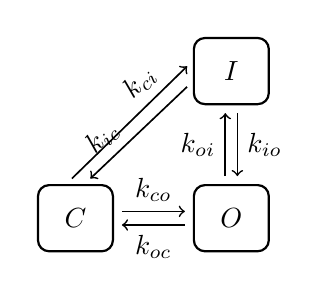
\begin{tikzpicture}[
   font=\sffamily,
   every matrix/.style={ampersand replacement=\&,column sep=1cm,row sep=1cm},
   state/.style={draw,thick,rounded corners,inner sep=.3cm},
   to/.style={->,semithick,shorten >=0.1cm,shorten <=0.1cm},
   Q/.style={->,semithick,sloped,pos=0.700000,shorten >=0.1cm,shorten <=0.1cm},  
   every node/.style={auto}]
\matrix{
\&\node[state] (I) {\parbox{10pt}{\centerline{$I$}}};\\
\node[state] (C) {\parbox{10pt}{\centerline{$C$}}};\&\node[state] (O) {\parbox{10pt}{\centerline{$O$}}};\\
};
\draw[to]  (O.100) to node {$k_{oi}$} (I.260);
\draw[to]  (O.190) to node {$k_{oc}$} (C.350);
\draw[to]  (I.280) to node {$k_{io}$} (O.80);
\draw[Q]  (I.195) to node {$k_{ic}$} (C.75);
\draw[to]  (C.10) to node {$k_{co}$} (O.170);
\draw[Q]  (C.105) to node {$k_{ci}$} (I.165);
\end{tikzpicture}
\end{center}
\caption{Markov model including three possible states: open (O), closed (C), and
inactivated (I).}
\label{Ionchannels_L:ICO}
\end{figure}


%FIGURE: [fig/Ionchannels_L_ICO.pdf, width=500 frac=0.8] Markov model including three possible states; open (O),  closed (C) and inactivated (I). label{Ionchannels_L:ICO}\subsection{Equilibrium probabilities}

We saw above (see page \pageref{eq_prob_ioc}) that the  equilibrium state of the
reaction shown in Figure  \ref{Ionchannels_L:ICO} is given by
\begin{align*}
o  &  =\frac{1}{1+\frac{k_{oc}}{k_{co}}+\frac{k_{oi}}{k_{io}}},\\
c  &  =\frac{\frac{k_{oc}}{k_{co}}}{1+\frac{k_{oc}}{k_{co}}+\frac{k_{oi}
}{k_{io}}},\\
i  &  =\frac{\frac{k_{oi}}{k_{io}}}{1+\frac{k_{oc}}{k_{co}}+\frac{k_{oi}
}{k_{io}}}.
\end{align*}


These probabilities are graphed as functions of the transmembrane potential in Figure
\ref{V:eq}. Note that the open probability in equilibrium is quite small; the channel is basically closed
for $v$ close to zero and it is inactivated for large values of $v$.

FIGURE: [fig/V_eq.pdf, width=500 frac=0.8] Equilibrium probabilities of the open, closed, and inactivated states as functions of the transmembrane potential $v$. label{V:eq}

\section{Probability density functions in the presence of the inactivated
state \label{pdfi}}

When the inactivated state is included in the model, as indicated in Figure  \ref{Ionchannels_L:ICO},
 the system governing the associated probability density functions is given by
\begin{align}
\frac{\partial\rho_{o}}{\partial t}+\frac{\partial}{\partial v}\left(
a_{o}\rho_{o}\right)   &  =k_{co}\rho_{c}-(k_{oc}+k_{oi})\rho_{o}+k_{io}
\rho_{i},\label{vpdfi1}\\
\frac{\partial\rho_{c}}{\partial t}+\frac{\partial}{\partial v}\left(
a_{c}\rho_{c}\right)   &  =k_{oc}\rho_{o}-(k_{co}+k_{ci})\rho_{c}+k_{ic}
\rho_{i},\label{vpdfi2}\\
\frac{\partial\rho_{i}}{\partial t}+\frac{\partial}{\partial v}\left(
a_{c}\rho_{i}\right)   &  =k_{oi}\rho_{o}-(k_{io}+k_{ic})\rho_{i}+k_{ci}
\rho_{c}\label{vpdfi3},
\end{align}
where
\begin{align}
a_{o}  &  =-g_{L}\left(  v-V_{L}\right)  -(v-V_{i})=\frac{11}{10}\left(
1-v\right)  ,\label{vfluxi}\\
a_{c}  &  =-g_{L}\left(  v-V_{L}\right)  =-\frac{1}{10}v.\nonumber
\end{align}


\subsection{Numerical simulations}
Again, we want to compare the solution computed by Monte Carlo simulations based on the stochastic
differential equation given in (\ref{v1b}) and the probability density functions defined by the system  (\ref{vpdfi1})--(\ref{vpdfi3}).
The numerical results are given in their usual form in Figure \ref{V:ioc}. 
As expected, the histograms computed using Monte Carlo simulations
and the numerical solution of the system  (\ref{vpdfi1})--(\ref{vpdfi3}) are quite similar. In these computations, 
the stochastic simulation ran for 100 s, with $\Delta t=0.01$ ms, and we used the mesh size $\Delta v=0.01$ in the numerical solution of the system  (\ref{vpdfi1})--(\ref{vpdfi3}). It is particularly interesting to
see that the tiny boundary layer close to $v=0$ for the probability density function of the inactivated state is captured using both the Monte Carlo and the probability density function approaches.


FIGURE: [fig/V_ioc.pdf, width=500 frac=0.8] Probability density functions of the open, closed, and inactivated states
(red lines) computed as numerical solutions of the system (\ref{vpdfi1})--(\ref{vpdfi3}) and
histograms based on Monte Carlo simulations using the stochastic differential
equation (\ref{v1b}). 
%{\bf xxx Glenn: is this the stationary solution of the pde?}. \G{yes.}
 label{V:ioc}
\section[Mutations affecting inactivation]{Mutations affecting the inactivated state of the ion channel}
\label{mutaffectinactiv}

Certain mutations of the sodium channel are known to impair the
channel's ability to deactivate. We introduce a mutation severity index $\mu$
and assume that the reaction rates of the mutant are changed such that both
the probabilities of moving from the inactivated to the closed state and from the 
inactivated to the open state are increased. The effect of these changes will clearly be to lower 
the probability of the channel being in the inactivated state.

In mathematical terms, we define
\begin{align}
\bar{k}_{ic} &  =\mu k_{ic},\label{ratesvm}\\
\bar{k}_{io} &  =\mu k_{io}, \nonumber
\end{align}
where $\mu\geqslant1$ and where $k_{ic}$ and $k_{io}$ are the wild type
reaction rates given by (ref{ratesv}) It should be noted that the
new reaction rates still satisfy the principle of detailed balance. 
%\K{zzz Jeg er litt usikker p\r{a} hva som menes med den forrige setningen.
%$k_{io}$ forandres ikke, men $\bar{k}_{io}$ er jo ikke lik $k_{io}$.
%Er poenget at ''the principle of detailed balance'' fortsatt gjelder selv
%om vi bruker $\bar{k}_{ic}$ og $\bar{k}_{io}$ i stedet for $k_{ic}$ og $k_{io}$?}
% \A{Corrected}
In Figure \ref{V:mu_ioc}, we show the equilibrium
probability density functions of the open, closed, and inactivated states for 
the wild type and for three values of the mutation severity index $\mu.$

FIGURE: [fig/V_mu_ioc.pdf, width=500 frac=0.8] Probability density functions of the open, closed, and 
inactivated states for the wild type and for three values of the mutation 
severity index: $\mu=1.5,\, 3,\, 10.$ Larger values of $\mu$ give
solutions farther away from the wild type solution (solid line). The probability density of the closed state is 
only shown for $v$ between 0 and 0.1 to magnify very small differences. label{V:mu_ioc}

\section[Drug for mutations of inactivation]{A theoretical drug for mutations affecting the inactivation}


We want to derive a theoretical drug repairing the effect of the mutation described in (\ref{ratesvm}). In the Markov model
illustrated in Figure  \ref{Ionchannels_L:BICO}, we have introduced a blocked state associated with the open, closed, and inactivated state and
we now want to figure out what the best choice might be.
The equilibrium solution of the reaction represented in Figure \ref{Ionchannels_L:BICO} is characterized by the equations
\begin{align*}
k_{co}c &  =k_{oc}o,\, k_{ci}c   =k_{ic}i,\\
k_{oi}o &  =k_{io}i,\, k_{bc}b_{c}   =k_{cb}c,\\
k_{bo}b_{o} &  =k_{ob}o, \, k_{bi}b_{i}   =k_{ib}i.
\end{align*}
It is useful to define
\[
r_{xy}=\frac{k_{xy}}{k_{yx}}
\]
and to note that
\[
r_{xy}=\frac{1}{r_{yx}}.
\]
With this notation, the principle of detailed balance stating that
\[
\frac{k_{co}k_{oi}k_{ic}}{k_{oc}k_{io}k_{ci}}=1
\]
can be written as
\[
r_{co}r_{oi}r_{ic}=r_{oc}r_{io}r_{ci}=1.
\]
The equations above can now be written as
\begin{align*}
c &  =r_{oc}o,\, c   =r_{ic}i,\\
o &  =r_{io}i,\, b_{c}   =r_{cb}c,\\
b_{o} &  =r_{ob}o,\, b_{i}   =r_{ib}i.
\end{align*}
It is convenient to express all probabilities in terms of the open probability:
\begin{align*}
c &  =r_{oc}o,\\
i &  =r_{oi}o,\\
b_{c} &  =r_{cb}c=r_{cb}r_{oc}o,\\
b_{o} &  =r_{ob}o,\\
b_{i} &  =r_{ib}i=r_{ib}r_{oi}o.
\end{align*}
Since $c+i+o+b_{c}+b_{o}+b_{i}=1,$ we have
\[
o=p^{-1},
\]
where
\[
p    =1+r_{oc}\left(  1+r_{cb}\right)  +r_{oi}\left(  1+r_{ib}\right)  +r_{ob}.
\]
We refer to $p$ as the inverse open probability and we note that for the wild type
it is given by
\[
p=1+r_{oc}+r_{oi}.
\]

\begin{figure}[ptb]
\begin{center}
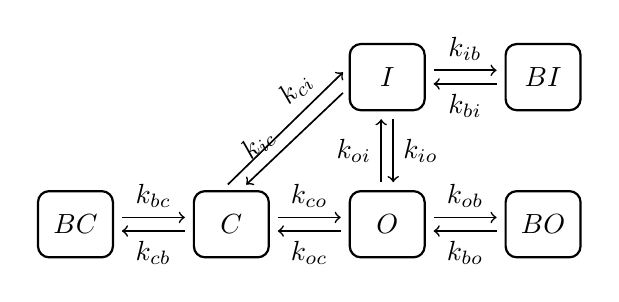
\begin{tikzpicture}[
   font=\sffamily,
   every matrix/.style={ampersand replacement=\&,column sep=1cm,row sep=1cm},
   state/.style={draw,thick,rounded corners,inner sep=.3cm},
   to/.style={->,semithick,shorten >=0.1cm,shorten <=0.1cm},
   Q/.style={->,semithick,sloped,pos=0.700000,shorten >=0.1cm,shorten <=0.1cm},  
   every node/.style={auto}]
\matrix{
\&\&\node[state] (I) {\parbox{10pt}{\centerline{$I$}}};\&\node[state] (BI) {\parbox{10pt}{\centerline{$BI$}}};\\
\node[state] (BC) {\parbox{10pt}{\centerline{$BC$}}};\&\node[state] (C) {\parbox{10pt}{\centerline{$C$}}};\&\node[state] (O) {\parbox{10pt}{\centerline{$O$}}};\&\node[state] (BO) {\parbox{10pt}{\centerline{$BO$}}};\\
};
\draw[to]  (O.100) to node {$k_{oi}$} (I.260);
\draw[to]  (O.190) to node {$k_{oc}$} (C.350);
\draw[to]  (O.10) to node {$k_{ob}$} (BO.170);
\draw[to]  (I.280) to node {$k_{io}$} (O.80);
\draw[Q]  (I.195) to node {$k_{ic}$} (C.75);
\draw[to]  (I.10) to node {$k_{ib}$} (BI.170);
\draw[to]  (C.10) to node {$k_{co}$} (O.170);
\draw[Q]  (C.105) to node {$k_{ci}$} (I.165);
\draw[to]  (C.190) to node {$k_{cb}$} (BC.350);
\draw[to]  (BO.190) to node {$k_{bo}$} (O.350);
\draw[to]  (BI.190) to node {$k_{bi}$} (I.350);
\draw[to]  (BC.10) to node {$k_{bc}$} (C.170);
\end{tikzpicture}
\end{center}
\caption{The model represented in Figure \ref{Ionchannels_L:ICO} extended 
to account for blockers associated with the closed state (BC), 
the open state (BO), and inactivated state (BI).}
\label{Ionchannels_L:BICO}
\end{figure}

%FIGURE: [fig/Ionchannels_L_BICO.pdf, width=500 frac=0.8] The model represented in Figure \ref{Ionchannels_L:ICO} extended to account for 
%blockers associated the closed state (BC), the open state (O) and the inactivated state (BI). label{Ionchannels_L:BICO}\subsection{Open probability in the mutant case }

As discussed above, we are interested in understanding how to define a
theoretical drug for mutations affecting the inactivation of the ion channel.
 We assume that the mutation affects the inactivation in a way that reduces the
probability of being in the inactivated state.  As mentioned above, this can be modeled by increasing
the reaction rates from the inactivated state to both the closed and the open states. We assume that
\[
\bar{k}_{ic}=\mu k_{ic},\text{ }\bar{k}_{io}=\mu k_{io},
\]
where $\mu\geqslant1$ is the mutation severity index.
This gives
\[
\bar{r}_{ic}=\frac{\bar{k}_{ic}}{k_{ci}}=\mu r_{ic}
\]
and
\[
\bar{r}_{io}=\frac{\bar{k}_{io}}{k_{oi}}=\mu r_{io}.
\]
We assume that the reaction rates between the closed and open states are
unaffected by the mutation and therefore
\[
\bar{r}_{oc}=r_{oc}.
\]
Detailed balance dictates that we should have
\[
(\mu k_{ic}) k_{co} k_{oi} = (\mu k_{io}) k_{oc} k_{ci},
\] 
which holds regardless of the choice of $\mu$, since the wild type rates satisfy the
principle of detailed balance.

The inverse open probability in the presence of the mutations is given by
\[
\bar{p}=1+r_{oc}+\bar{r}_{oi}=1+r_{oc}+1/\bar{r}_{io} =1+r_{oc}+\frac{1}{\mu r_{io}}
 = 1+r_{oc}+\frac{r_{oi}}{\mu}.
\]

%%%%%%%%%%%%%%%%%%%%%%%%%%%%%%%%%%%%%%%%%%

\subsection{The open probability in the presence of the theoretical drug}

When the drug given in Figure \ref{Ionchannels_L:BICO} is applied, the inverse open probability is
\[
p_{b}=1+r_{oc}\left(  1+r_{cb}\right)  +\frac{r_{oi}}{\mu}\left(
1+r_{ib}\right)  +r_{ob}
\]
where $r_{cb},r_{ib}$, and $r_{ob}$ are used to characterize the drug. Our aim
is to now use these parameters to tune the drug such that
\[
p_{b}\approx p,
\]
where $p$ is the inverse open probability of the wild type. More precisely, we
want to determine the constants $r_{cb},r_{ib}$, and $r_{ob}$ such that
\[
1+r_{oc}\left(  1+r_{cb}\right)  +\frac{r_{oi}}{\mu}\left(  1+r_{ib}\right)
+r_{ob}\approx1+r_{oc}+r_{oi}
\]
holds for all relevant values of the transmembrane potential $v.$ We observe
that if we put $r_{cb}=r_{ob}=0,$ we obtain the condition
\[
\frac{r_{oi}}{\mu}\left(  1+r_{ib}\right)  \approx r_{oi}
\]
and therefore we set
\[
r_{ib}=\mu-1.
\]
We conclude that we can repair the equilibrium state of the mutation
completely by applying a drug consisting of a blocker of the inactivated
state, provided that the reaction rates of the drug satisfy
\[
\frac{k_{ib}}{k_{bi}}=\mu-1,
\]
where $\mu$ is the severity index of the mutation. This means that we have
reduced the problem of finding a drug to a single parameter given by
$k_{bi}.$ This remaining degree of freedom will be addressed below.


\section[PDFs: blocked inactivated state]{Probability density functions using the blocker of the inactivated state}

\begin{figure}[ptb]
\begin{center}
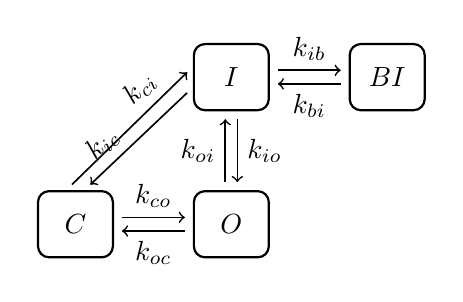
\begin{tikzpicture}[
   font=\sffamily,
   every matrix/.style={ampersand replacement=\&,column sep=1cm,row sep=1cm},
   state/.style={draw,thick,rounded corners,inner sep=.3cm},
   to/.style={->,semithick,shorten >=0.1cm,shorten <=0.1cm},
   Q/.style={->,semithick,sloped,pos=0.700000,shorten >=0.1cm,shorten <=0.1cm},  
   every node/.style={auto}]
\matrix{
\&\node[state] (I) {\parbox{10pt}{\centerline{$I$}}};\&\node[state] (BI) {\parbox{10pt}{\centerline{$BI$}}};\\
\node[state] (C) {\parbox{10pt}{\centerline{$C$}}};\&\node[state] (O) {\parbox{10pt}{\centerline{$O$}}};\&\\
};
\draw[to]  (O.100) to node {$k_{oi}$} (I.260);
\draw[to]  (O.190) to node {$k_{oc}$} (C.350);
\draw[to]  (I.280) to node {$k_{io}$} (O.80);
\draw[Q]  (I.195) to node {$k_{ic}$} (C.75);
\draw[to]  (I.10) to node {$k_{ib}$} (BI.170);
\draw[to]  (C.10) to node {$k_{co}$} (O.170);
\draw[Q]  (C.105) to node {$k_{ci}$} (I.165);
\draw[to]  (BI.190) to node {$k_{bi}$} (I.350);
\end{tikzpicture}
\end{center}
\caption{Markov model of the prototype ion channel with a blocker associated with the inactivated state.}
\label{Ionchannels_L:BICO4}
\end{figure}



%FIGURE: [fig/Ionchannels_L_BICO4.pdf, width=500 frac=0.8] Markov model of the prototype ion channel with a blocker associated with the inactivated state. label{Ionchannels_L:BICO4}In Section \ref{pdfi} above, we derived a system governing the probability density
functions of the open, closed, and inactivated states. Here, we want to extend
the system to account for the theoretical drug represented by a blocker of the
inactivated state. The Markov model of the drug is given in Figure \ref{Ionchannels_L:BICO4}. The drug will
completely repair the equilibrium state of the Markov model, provided that
\begin{equation}
k_{ib}=\left(  \mu-1\right)  k_{bi}\label{kib},
\end{equation}
where $\mu$ is the mutation severity index of the mutation (see (\ref{ratesvm})). The
stationary probability density functions of the states in the Markov model of
Figure \ref{Ionchannels_L:BICO4} are governed by the system
\begin{align}
\frac{\partial}{\partial v}\left(  a_{o}\rho_{o}\right)   &  =k_{co}\rho
_{c}-\left(  k_{oc}+ k_{oi}\right)  \rho_{o}+\mu k_{io}\rho
_{i},\label{bvpdfi1}\\
\frac{\partial}{\partial v}\left(  a_{c}\rho_{c}\right)   &  =k_{oc}\rho
_{o}-\left(  k_{co}+ k_{ci}\right)  \rho_{c}+\mu k_{ic}\rho
_{i},\label{bvpdfi2}\\
\frac{\partial}{\partial v}\left(  a_{c}\rho_{i}\right)   &  = k_{oi}\rho_{o}-(\mu k_{io}+\mu k_{ic}+\left(  \mu-1\right)  k_{bi})\rho_{i}
+k_{ci}\rho_{c}+k_{bi}\rho_{b},\label{bvpdfi3}\\
\frac{\partial}{\partial v}\left(  a_{c}\rho_{b}\right)   &  =\left(
\mu-1\right)  k_{bi}\rho_{i}-k_{bi}\rho_{b},\label{bvpdfi4}
\end{align}
%\K{zzz Jeg forst\r{a}r ikke hvorfor man her deler $k_{oi}$ og $k_{ci}$ p\r{a}
%$\mu$ i stedet for \r{a} gange $k_{io}$ og $k_{ic}$ med $\mu$.}
%\A{Error. Background: we played with different directions for the mutation. Fixed now. xxx Glenn: Make sure code act according to corrected text}
%\G{The code has the mutation in the correct place, as in (11.6).}
where $\rho_{o},\rho_{c},\rho_{i},$ and $\rho_{b}$ denote the probability density
functions of the open, closed, inactivated, and blocked states, respectively, 
and where the flux terms are given by
\begin{align*}
a_{o} &  =-g_{L}\left(  v-V_{L}\right)  -(v-V_{i})=\frac{11}{10}\left(
1-v\right)  ,\\
a_{c} &  =-g_{L}\left(  v-V_{L}\right)  =-\frac{1}{10}v.
\end{align*}
The associated model of the wild type is given by
\begin{align}
\frac{\partial}{\partial v}\left(  a_{o}\rho_{o}\right)   &  =k_{co}\rho
_{c}-\left(  k_{oc}+k_{oi}\right)  \rho_{o}+k_{io}\rho_{i},\label{pdf100}\\
\frac{\partial}{\partial v}\left(  a_{c}\rho_{c}\right)   &  =k_{oc}\rho
_{o}-\left(  k_{co}+k_{ci}\right)  \rho_{c}+k_{ic}\rho_{i},\label{pdf101}\\
\frac{\partial}{\partial v}\left(  a_{c}\rho_{i}\right)   &  =k_{oi}\rho
_{o}-(k_{io}+k_{ic})\rho_{i}+k_{ci}\rho_{c}.\label{pdf102}
\end{align}
All the reactions rates used in the computations are given in (\ref{ratesv}); the computational domain
is given by $\Omega=[0,1]$ and we used 201 mesh points. 
In Figure \ref{V:drug_ico}, we show the difference between the open state probability density
function of the wild type, denoted by $\rho_{o},$ computed by solving the
system ($\ref{pdf100}$)--($\ref{pdf102}$), and the mutant where the
drug is applied, computed by solving ($\ref{bvpdfi1}$)--($\ref{bvpdfi4}$), denoted by $\rho_{o}^{\ast}.$ The difference is defined by the norm
\begin{equation}
\Vert  \rho_{o}-\rho_{o}^{\ast}\Vert=\frac{\left\Vert \rho_{o}-\rho_{o}^{\ast}\right\Vert _{L^{2}\left(
\Omega\right)  }}{\left\Vert \rho_{o}\right\Vert _{L^{2}\left(  \Omega\right)
}+\left\Vert \rho_{o}^{\ast}\right\Vert _{L^{2}\left(  \Omega\right)  }}, \label{normfrac}
\end{equation}
where, as usual,
\[
\left\Vert \rho\right\Vert _{L^{2}\left(  \Omega\right)  }=\left(
\int_{\Omega}\rho^{2}dv\right)  ^{1/2}.
\]
We observe that, as $k_{bi}$ increases, the drug defined by $\left(
\ref{kib}\right)  $ completely repairs the effect of the mutation.

FIGURE: [fig/V_drug_ico.pdf, width=500 frac=0.8] The difference between the open probability density function
of the wild type ($\rho$) and the open probability density function ($\rho^\ast$) of the mutant using the drug defined by
(\ref{kib}), measured by the norm $\Vert  \rho_{o}-\rho_{o}^{\ast}\Vert$ defined in  (\ref{normfrac}). The difference
goes to zero as the parameter $k_{bi}$ is increased. label{V:drug_ico}

%\section{Notes}

%\begin{itemize}
%\item The functions and parameters of (\ref{ratesv}) is motivated by xxxGlenn: where did you get it? referencexxx. \G{Somewhat arbitrarily, st{\aa}r det n{\aa}. Det stemmer bra. Brukte muligens Clancy som inspirasjon, men ikke til aa kjenne igjen naa.}
%\end{itemize}



\chapter{A simple model of the sodium channel \label{simple_Na}}

In the previous two chapters, we studied a prototypical model of an ion
channel. The model consisted of a differential equation involving a gating
mechanism that could be either open or closed. A Markov model governed the
gating and we derived a system giving the probability density functions of
the states involved in the Markov model. We used the probability density
approach to compute optimal theoretical drugs and noted that a mutation
leading to an increase in the closed to open reaction rate could be completely
repaired by an optimal closed state drug.

Next, we extended the prototypical model to also include an inactivated state.
The inactivated state can also be affected by mutations and we studied the
particular case in which the rates from inactivated to open and from 
inactivated to closed were increased by a factor $\mu$ referred to as the 
mutation severity index. In this case, we observed that an optimal drug was 
represented by a blocker associated with the inactivated state. We were again
able to completely repair the effect of the mutation using the theoretical
 drug.

In this chapter, we shall move closer to realistic Markov models of sodium
channels. These models tend to be somewhat more intricate than the
prototypical model we have studied so far. Providing Markov models of the
sodium channels has been a very active field of research for decades and a
series of models are available. We have chosen to study models that seem to
capture the basic structure applied in many models but are manageable from a
mathematical point of view. We choose this approach for clarity of
presentation and not for its ability to represent specific data. It is,
hopefully, quite clear that the method we use to analyze the models is
applicable to many other models.

Mutations of the sodium channel can lead to impaired inactivation. This may
lead to leakage of the sodium current, which can again trigger arrhythmias.
Here we will consider a model of the $\Delta$KPQ mutation of the SCN5A gene.
This mutation may lead to an arrhythmogenic disorder referred to as the long-QT
syndrome, which can lead to sudden cardiac death in the worst case. There are
several models representing the effect of the $\Delta$KPQ mutation. 
One that is well known is
provided by Clancy and Rudy \cite{Clancy1999}. Their approach to model the
impaired inactivation is to introduce a burst mode in the model where no
inactivation state is available. We will consider two ways of modeling the
effect of the mutation.

 In the first approach, we will use the method
utilized above. We will simply increase the reaction rate from the inactivated
to the closed state and from the inactivated to the open state by a factor
$\mu\ge1$, referred to as the mutation severity index. This change will clearly
reduce the probability of being in the inactivated state. 
It is therefore a model of impaired inactivation.

The second approach is
to introduce a burst mode in the model. When the channel is in the burst mode,
there is no inactivated state. This model will be
parameterized such that it is highly unlikely that the channel will enter the
burst mode for the wild type case, but the probability of entering the burst
mode is considerably higher in the mutant case.

\section{Markov model of a wild type sodium channel}

Markov models have turned out to be a powerful tool in representing the physics
of the sodium channel and a series of alternatives have been proposed by
various authors. Since this is still a very active field of research, it is hard
to claim one particular model as the definitive model. We
shall therefore focus on a kind of model that has a structure that seems to
be more or less agreed upon but, as usual, we attack this problem with
simplicity in mind. This also holds true for the way we introduce the effect
of a mutation.

We start by considering a simple model of the sodium channel, illustrated in
Figure \ref{wtreac}. The actual functions used in our computations will be
given below. However, we should note that the functions will always be chosen
such that they satisfy the principle of detailed balance, which, for the model
given in Figure \ref{wtreac}, means that the following relation holds:%
\begin{equation}
k_{io}k_{oc}k_{ci}=k_{oi}k_{ic}k_{co}. \label{db2}%
\end{equation}
The model of the closed states deserves a comment or two. Let us assume that a
sodium channel consists of three subunits and these subunits may exist in two
states: closed or permissible. The whole channel is in the state $C_{0}$ if
all three units are in the permissible state. Over a brief period given
by $\Delta t$, the channel can change from the state $C_{0}$ to the open
state and the probability of this event is $\Delta t k_{co}$ or it can
change to the inactivated state with probability $\Delta t k_{ci}$. However, the
channel can also go from the permissible state $C_{0}$ to the state $C_{1}$ and 
the probability of doing this is $3\Delta t \beta$. The reason for the factor 
of three here is that it is sufficient that one of the three subunits closes. By
assuming that the subunits act independently, we find that the probability is
$3\Delta t \beta$. The same reasoning gives us the rest of the
transitions between the different closed states.

\begin{figure}[ptb]
\begin{center}
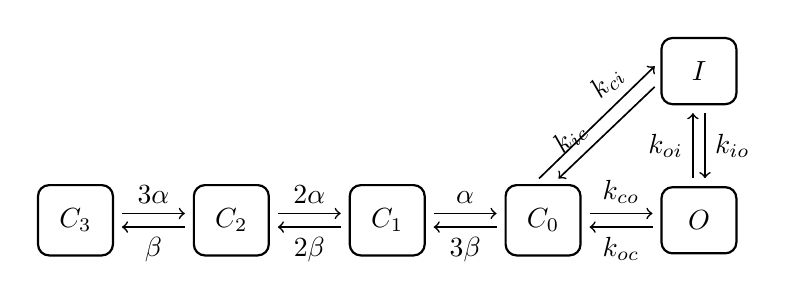
\begin{tikzpicture}[
   font=\sffamily,
   every matrix/.style={ampersand replacement=\&,column sep=1cm,row sep=1cm},
   state/.style={draw,thick,rounded corners,inner sep=.3cm},
   to/.style={->,semithick,shorten >=0.1cm,shorten <=0.1cm},
   Q/.style={->,semithick,sloped,pos=0.700000,shorten >=0.1cm,shorten <=0.1cm}, 
   every node/.style={auto}]
\matrix{
\&\&\&\&\node[state] (I) {\parbox{10pt}{\centerline{$I$}}};\\
\node[state] (C_{3}) {\parbox{10pt}{\centerline{$C_{3}$}}};\&\node[state] (C_{2}) {\parbox{10pt}{\centerline{$C_{2}$}}};\&\node[state] (C_{1}) {\parbox{10pt}{\centerline{$C_{1}$}}};\&\node[state] (C_{0}) {\parbox{10pt}{\centerline{$C_{0}$}}};\&\node[state] (O) {\parbox{10pt}{\centerline{$O$}}};\\
};
\draw[to]  (O.100) to node {$k_{oi}$} (I.260);
\draw[to]  (O.190) to node {$k_{oc}$} (C_{0}.350);
\draw[to]  (I.280) to node {$k_{io}$} (O.80);
\draw[Q]  (I.195) to node {$k_{ic}$} (C_{0}.75);
\draw[to]  (C_{0}.10) to node {$k_{co}$} (O.170);
\draw[Q]  (C_{0}.105) to node {$k_{ci}$} (I.165);
\draw[to]  (C_{0}.190) to node {$3\beta$} (C_{1}.350);
\draw[to]  (C_{1}.10) to node {$\alpha$} (C_{0}.170);
\draw[to]  (C_{1}.190) to node {$2\beta$} (C_{2}.350);
\draw[to]  (C_{2}.10) to node {$2\alpha$} (C_{1}.170);
\draw[to]  (C_{2}.190) to node {$\beta$} (C_{3}.350);
\draw[to]  (C_{3}.10) to node {$3\alpha$} (C_{2}.170);
\end{tikzpicture}
\end{center}
\caption{Markov model of a wild type sodium channel consisting of an open
state $(O)$, an inactivated state $(I)$, and four closed states $(C_{0}%
,C_{1},C_{2},C_{3})$.}%
\label{wtreac}%
\end{figure}


\subsection{The equilibrium solution}

The equilibrium probabilities of the model given in Figure \ref{wtreac} are
characterized by the equations%
\[%
\begin{array}
[c]{ccc}%
k_{ci}c_{0}=k_{ic}i, & k_{oi}o=k_{io}i, & k_{co}c_{0}=k_{oc}o,\\
3\beta c_{0}=\alpha c_{1}, & 2\alpha c_{2}=2\beta c_{1}, & 3\alpha c_{3}=\beta
c_{2},
\end{array}
\]
where $c_{0}$ denotes the equilibrium probability of being in the state
$C_{0}$. Similarly, the other variables are defined as the equilibrium
probability of being in the states $C_{1},C_{2},C_{3},I$, and $O$. We express all
probabilities in terms of the open probability:%
\begin{align*}
i  &  =\frac{k_{oi}}{k_{io}}o,\text{ }c_{0}=\frac{k_{oc}}{k_{co}}o,\text{ }\\
c_{1}  &  =\frac{3\beta}{\alpha}\frac{k_{oc}}{k_{co}}o,\text{ }c_{2}%
=\frac{3\beta^{2}}{\alpha^{2}}\frac{k_{oc}}{k_{co}}o,\text{ }c_{3}=\frac
{\beta^{3}}{\alpha^{3}}\frac{k_{oc}}{k_{co}}o.
\end{align*}
Since $o+i+c_{0}+c_{1}+c_{2}+c_{3}=1,$ we find the following equilibrium probabilities:%

\begin{align}
o  &  =\frac{1}{q_{w}},\text{ }i=\frac{k_{oi}/k_{io}}{q_{w}},\text{ }%
c_{0}=\frac{k_{oc}/k_{co}}{q_{w}}, \label{prob_wt}\\
c_{1}  &  =\frac{3\beta}{\alpha}\frac{k_{oc}/k_{co}}{q_{w}},\text{ }%
c_{2}=\frac{3\beta^{2}}{\alpha^{2}}\frac{k_{oc}/k_{co}}{q_{w}},\text{ }%
c_{3}=\frac{\beta^{3}}{\alpha^{3}}\frac{k_{oc}/k_{co}}{q_{w}},\nonumber
\end{align}
where%
\[
q_{w}=1+\frac{k_{oi}}{k_{io}}+\frac{k_{oc}}{k_{co}}\left(  1+\beta
/\alpha\right)  ^{3}.
\]
Here the subscript $w$ is used to indicate that $q_{w}$ represents the 
wild type case.

\section{Modeling the effect of a mutation impairing the inactivated state}

The mutation impairs the inactivated state of the channel. In Section
\ref{mutaffectinactiv} we modeled this by increasing the probability of moving
from the inactivated state to the open state or to the closed state. This was
done by increasing the rates $k_{io}$ and $k_{ic}.$ We use the same approach
here and define%
\begin{align}
\bar{k}_{ic}  &  =\mu k_{ic},\label{kic1}\\
\bar{k}_{io}  &  =\mu k_{io}, \label{kio2}%
\end{align}
where, as usual, $\mu$ is the mutation severity index. From (\ref{db2}), we
have
\[
k_{io}k_{oc}k_{ci}=k_{ic}k_{co}k_{oi}%
\]
and therefore%
\[
\left(  \mu k_{io}\right)  k_{oc}k_{ci}=\left(  \mu k_{ic}\right)
k_{co}k_{oi};%
\]
so%
\[
\bar{k}_{io}k_{oc}k_{ci}=\bar{k}_{ic}k_{co}k_{oi}%
\]
and thus the principle of detailed balance also holds for the mutant case,
in which the rates are given by $(\ref{kic1})$ and $(\ref{kio2}).$

\subsection{The equilibrium probabilities}
The reaction scheme of the mutant is illustrated in Figure \ref{mtreac}. In
the mutant case, the equilibrium probabilities are given by%
\begin{align}
o  &  =\frac{1}{q_{m}},\text{ }i=\frac{k_{oi}/\left(  \mu k_{io}\right)
}{q_{m}},\text{ }c_{0}=\frac{k_{oc}/k_{co}}{q_{m}}, \\
c_{1}  &  =\frac{3\beta}{\alpha}\frac{k_{oc}/k_{co}}{q_{m}},\text{ }%
c_{2}=\frac{3\beta^{2}}{\alpha^{2}}\frac{k_{oc}/k_{co}}{q_{m}},\text{ }%
c_{3}=\frac{\beta^{3}}{\alpha^{3}}\frac{k_{oc}/k_{co}}{q_{m}}, \nonumber
\end{align}
where%
\[
q_{m}=1+\frac{k_{oi}}{\mu k_{io}}+\frac{k_{oc}}{k_{co}}\left(  1+\beta
/\alpha\right)  ^{3}.
\]
For the equilibrium state it is worth observing that, since
\[
i=\frac{k_{oi}/k_{io}}{\frac{k_{oi}}{k_{io}}+\mu\left(  1+\frac{k_{oc}}%
{k_{co}}\left(  1+\beta/\alpha\right)  ^{3}\right)  },%
\]
the probability of being in the inactivated state is reduced when $\mu$ is
increased. Similarly, we observe that the associated open probability given
by%
\[
o=\frac{1}{1+\frac{k_{oi}}{\mu k_{io}}+\frac{k_{oc}}{k_{co}}\left(
1+\beta/\alpha\right)  ^{3}}%
\]
increases as $\mu$ increases. Although these calculations concern the 
equilibrium state, this is a pretty strong hint of an increased open 
probability in the dynamic case as well and an increased open probability is 
exactly the problem one observes when inactivation is impaired.

\begin{figure}[ptb]
\begin{center}
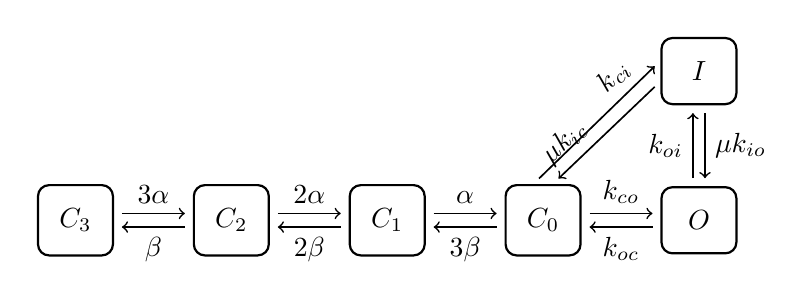
\begin{tikzpicture}[
   font=\sffamily,
   every matrix/.style={ampersand replacement=\&,column sep=1cm,row sep=1cm},
   state/.style={draw,thick,rounded corners,inner sep=.3cm},
   to/.style={->,semithick,shorten >=0.1cm,shorten <=0.1cm},
   Q/.style={->,semithick,sloped,pos=0.750000,shorten >=0.1cm,shorten <=0.1cm},  
   every node/.style={auto}]
\matrix{
\&\&\&\&\node[state] (I) {\parbox{10pt}{\centerline{$I$}}};\\
\node[state] (C_{3}) {\parbox{10pt}{\centerline{$C_{3}$}}};\&\node[state] (C_{2}) {\parbox{10pt}{\centerline{$C_{2}$}}};\&\node[state] (C_{1}) {\parbox{10pt}{\centerline{$C_{1}$}}};\&\node[state] (C_{0}) {\parbox{10pt}{\centerline{$C_{0}$}}};\&\node[state] (O) {\parbox{10pt}{\centerline{$O$}}};\\
};
\draw[to]  (O.100) to node {$k_{oi}$} (I.260);
\draw[to]  (O.190) to node {$k_{oc}$} (C_{0}.350);
\draw[to]  (I.280) to node {$\mu k_{io}$} (O.80);
\draw[Q]  (I.195) to node {$\mu k_{ic}$} (C_{0}.75);
\draw[to]  (C_{0}.10) to node {$k_{co}$} (O.170);
\draw[Q]  (C_{0}.105) to node {$k_{ci}$} (I.165);
\draw[to]  (C_{0}.190) to node {$3\beta$} (C_{1}.350);
\draw[to]  (C_{1}.10) to node {$\alpha$} (C_{0}.170);
\draw[to]  (C_{1}.190) to node {$2\beta$} (C_{2}.350);
\draw[to]  (C_{2}.10) to node {$2\alpha$} (C_{1}.170);
\draw[to]  (C_{2}.190) to node {$\beta$} (C_{3}.350);
\draw[to]  (C_{3}.10) to node {$3\alpha$} (C_{2}.170);
\end{tikzpicture}
\end{center}
\caption{Markov model of the mutant version of the sodium channel consisting of
an open state $(O)$, an inactivated state $(I)$, and four closed states
$(C_{0},C_{1},C_{2},C_{3})$. Here $\mu$ is referred to as the mutation
severity index.}%
\label{mtreac}%
\end{figure}

\bigskip


\section{Stochastic model of the sodium channel}




We use the same model of the transmembrane potential as above (see
(\ref{v1}) on page \pageref{v1}). Recall that the stochastic differential equation is
given by%
\begin{equation}
Cv^{\prime}=-g_{L}\left(  v-V_{L}\right)  -\gamma g_{Na}(v-V_{Na}), \label{sv1}%
\end{equation}
\graytable{l}{
{|c|c|} \hline
$C$ &  $1$ $\mu\text{F/cm}^{2}$\\ \hline
$g_L$ & $1/10 \text{ mS/cm}^{2}$ \\ \hline
$g_{Na}$ & $1\text{ mS/cm}^{2}$ \\ \hline
$V_L$ & $-85\text{ mV}$ \\ \hline
$V_{Na}$ & $45\text{ mV}$\\ \hline
}{Values of the parameters used in model \ref{sv1}.\label{scoef}}
where $C$ is the capacitance of the membrane, $V_{L}$ is the resting potential
of the leakage current, and $V_{Na}$ is the resting potential of the sodium
channel. The parameters are listed in Table \ref{scoef}.


%We use the following parameters:
%\begin{align}
%C  &  =1\mu\text{F/cm}^{2},\nonumber\\
%g_{L}  &  =\frac{1}{10}\text{mS/cm}^{2},\nonumber\\
%g_{Na}  &  =1\text{mS/cm}^{2}\label{scoef}\\
%V_{L}  &  =-85\text{mV,}\nonumber\\
%V_{Na}  &  =45\text{mV.}\nonumber
%\end{align}
The sodium channel can be either open (O), with $\gamma=1,$ or closed (C), with
$\gamma=0,$ and, as usual, the state of the channel is determined by a Markov
model. Since $C=1,$ we rewrite the equation in the more convenient form%

\begin{equation}
v^{\prime}=-g_{L}\left(  v-V_{L}\right)  -\gamma g_{Na}(v-V_{Na}), \label{sv2}%
\end{equation}
where $g_{L}$ and $g_{Na}$ now have the unit\footnote{The use of the odd units for 
$g_{L}$ and $g_{Na}$ stems from the fact that we have, for notational
 convenience, incorporated the capacitance of the membrane in these constants.}
$\text{ms}^{-1}.$

\subsection{A numerical scheme with an invariant region}

A numerical scheme for the model $\left(  \ref{sv2}\right)  $ can be written
in the form%
\begin{equation}
v_{n+1}=v_{n}-\Delta t\left(  g_{L}\left(  v_{n}-V_{L}\right)  +\gamma
_{n}g_{Na}(v_{n}-V_{Na}\right)  ), \label{svs}%
\end{equation}
where $\gamma_{n}$ is either zero or one and where $\Delta t$ denotes the
time step. We assume that the condition%
\begin{equation}
\Delta t<\frac{1}{g_{L}+g_{Na}} \label{svdt}%
\end{equation}
holds and, under this condition, we will show that an invariant region for the solutions
generated by the scheme $\left(  \ref{svs}\right)  $ is given by%
\begin{equation}
\Omega=\left(  V_{L},V_{+}\right)  , \label{inv_region_2}%
\end{equation}
where%
\[
V_{+}=\frac{g_{L}V_{L}+g_{Na}V_{Na}}{g_{L}+g_{Na}}
\]
and, for the parameters we defined in $\left(  \ref{scoef}\right)  $, we have
$V_{+}\approx 33.18$ mV.
%\K{zzz xxxFor parametrene definert i (\ref{scoef}) f\r{a}r jeg 
%$V_{+}\approx 28.64$mV. Men dersom $V_{Na}=45$mV som det st\r{a}r i
%bildetekseten til Figure \ref{NaM/mc.pdf} stemmer det at $V_{+}\approx 33.18$mV.}\G{Har brukt  $V_{Na}=45$mV, endret til det i dokumentet}

To derive the invariant region, we proceed along the lines used on
page \pageref{vdt} and thus start by defining%
\[
H(v,\gamma)=v-\Delta t\left(  g_{L}\left(  v-V_{L}\right)  +\gamma
g_{Na}(v-V_{Na}\right)  ).
\]
For values of $v$ in the region $\Omega$ and for values of $\Delta t$
satisfying condition $\left(  \ref{svdt}\right)$, we have the properties%
\[
\frac{d}{dv}H(v,\gamma)=1-\Delta t\left(  g_{L}+\gamma g_{Na}\right)
\geqslant1-\Delta t\left(  g_{L}+g_{Na}\right)  >0
\]
and%
\[
\frac{d}{d\gamma}H(v,\gamma)=-\Delta t\left(  g_{Na}(v-V_{Na}\right)  )>0.
\]
Using these observations, we obtain%
\[
v_{n+1}=H(v_{n},\gamma_{n})\leqslant H(V_{+},1)=V_{+}%
\]
and%
\[
v_{n+1}=H(v_{n},\gamma_{n})\geqslant H(V_{L},0)=V_{L}.
\]
So, by induction, it holds that $\Omega=\left(  V_{L},V_{+}\right)  $ is an
invariant region for scheme $\left(  \ref{svs}\right)  .$


\section[Probability density functions]{Probability density functions for the
voltage-gated channel}
The systems modeling the probability density functions in the wild type 
and mutant cases are of exactly the same form; the only difference is
given by the mutation severity index. 
The probability density functions of the states of the Markov model given in
Figure \ref{mtreac} are given by%
\begin{align}
\frac{\partial\rho_{o}}{\partial t}+\frac{\partial}{\partial v}\left(
a_{o}\rho_{o}\right)   &  =k_{co}\rho_{0}-\left(  k_{oc}+k_{oi}\right)
\rho_{o}+\mu k_{io}\rho_{i},\nonumber\\
\frac{\partial\rho_{i}}{\partial t}+\frac{\partial}{\partial v}\left(
a_{c}\rho_{i}\right)   &  =k_{oi}\rho_{o}-\mu\left(  k_{io}+k_{ic}\right)
\rho_{i}+k_{ci}\rho_{0},\nonumber\\
\frac{\partial\rho_{0}}{\partial t}+\frac{\partial}{\partial v}\left(
a_{c}\rho_{0}\right)   &  =k_{oc}\rho_{o}-\left(  k_{ci}+k_{co}+3\beta\right)
\rho_{0}+\mu k_{ic}i +\alpha \rho_{1} ,\label{vgpdf}\\
\frac{\partial\rho_{1}}{\partial t}+\frac{\partial}{\partial v}\left(
a_{c}\rho_{1}\right)   &  =2\alpha\rho_{2}-\left(  \alpha+2\beta\right)
\rho_{1}+3\beta\rho_{0},\nonumber\\
\frac{\partial\rho_{2}}{\partial t}+\frac{\partial}{\partial v}\left(
a_{c}\rho_{2}\right)   &  =3\alpha\rho_{3}-\left(  2\alpha+\beta\right)
\rho_{2}+2\beta\rho_{1},\nonumber\\
\frac{\partial\rho_{3}}{\partial t}+\frac{\partial}{\partial v}\left(
a_{c}\rho_{3}\right)   &  =-3\alpha\rho_{3}+\beta\rho_{2},\nonumber
\end{align}
where
\begin{align}
a_{o} &  =-g_{L}\left(  v-V_{L}\right)  -g_{Na}(v-V_{Na}),\label{sflux}\\
a_{c} &  =-g_{L}\left(  v-V_{L}\right)  ,\nonumber
\end{align}
with $\rho_{o}$ denoting the probability density function of being in the open
state, $\rho_{0}$ denoting the probability density function of being in the
state $C_{0},$ and so on.
%\K{zzz I de to f\o rste ligningene i dette systemet blir det brukt 
%$\rho_{c_{0}}$ i stedet for $\rho_{0}$. Er det noen grunn til det? 
%Dessuten ville jeg tro at man i tillegg til det som st\r{a}r der
%skulle legge til leddene 
%$+\alpha \rho_{1} - 3\beta \rho_{0}$ 
%p\r{a} h\o yresiden i den tredje ligningen. 
%Er det noen grunn til at man ikke gj\o r det?}
%\A{Both corrected: xxx  Glenn: make sure you correct the code accordingly.}
%\G{This was correct in the code.}

\subsection{Model parameterization}

To carry out numerical computations comparing the properties
of the  wild type and the mutant sodium channel, we need to define
the rates involved in the model described in Figure \ref{mtreac}. We use the 
rates
\[  k_{ab}(v) = k^{\infty}_{ab}(v)/\tau_{ab}, \ \ \  k_{ba}(v) = (1-k^{\infty}_{ab}(v))/\tau_{ab}, \]
with
\[k^{\infty}_{ab} = \frac{1}{1+e^{s_{a\!b}(V_{a\!b}-v)}}. \]
Furthermore, the rates $\alpha$ and $\beta$ in Figure \ref{mtreac} are given by
\[
\alpha =k^{\infty}_{cp}/\tau_{cp}  \text{ and } \beta =(1-k^{\infty}_{cp})/\tau_{cp}.
\]
With this parameterization, the principle of detailed balance is satisfied, provided that
\[ 
s_{co} + s_{ic} + s_{oi}=0 \mbox{\ \ and\ \ } s_{co}V_{co} + s_{oi}V_{oi} + s_{ic}V_{ic}  =0.  \]
The parameters are given in Table \ref{markov_rates} and we introduce the mutation as we
did in the previous chapter: We increase the probability of going from the
inactivated state to either the open or the closed state. More specifically, we define
\[
\bar{k}_{ic} = \mu k_{ic}  \text{ and } \bar{k}_{io} = \mu k_{io},
\] where, as usual, the wild type case is given by $\mu=1$. 

\begin{table}  \begin{center}
\begin{tabular}{|r|r|r|r|} \hline
$ab$ & $V_{ab}$ (mV) & $s_{ab}$ (1/mV) &  $\tau_{ab}$ (ms)\\ \hline
$co$ & -60 & 0.1& 0.01\\ \hline
$oi$ & -120 & 0.05 & 3 \\  \hline
$ic$ & -80 & -0.15& 10\\ \hline
$cp$ &-60 & 0.1& 0.1\\ \hline
\end{tabular} \end{center}
\caption{Parameters of the Markov model illustrated in Figures \ref{wtreac} 
and \ref{mtreac}. 
%\K{zzz Skal man oppgi enheter for disse parametrene?}
} 
\label{markov_rates} 
\end{table}

\subsection{Numerical experiments comparing the properties of the wild type 
and the mutant sodium channel}



In Figure \ref{NaM/pdf3.pdf}, we show the
probability density functions of the open state, the inactivated state, and the
sum of the closed states for the wild type case $(\mu=1)$ and two mutations
$(\mu=10$ and $\mu=30).$ The properties of the solutions are summarized in
Table \ref{na_stat}, which presents the expected values of the open state, the
inactivated state, and the sum of the closed states.


\fig{NaM/pdf3.pdf}{The probability density functions of the open state (left),
the sum of the closed states  (center), and the inactivated state (right) 
for the wild type case (solid line) and two values of the mutation severity 
index: $\mu=10$ and $\mu=30$. The strongest mutation differs the most
from the wild type solution. 
%{\bf xxx Glenn: something wrong here - read text and compare with headings of figures} \G{yes, fixed now.}
}

%\begin{table}  \begin{center}
%\begin{tabular}{|r|r|r|r|} \hline
%$\mu$ & $E_o$ & $E_i$ & $E_c$ \\ \hline
%1 & -50.8 & -84.9 & -83.5 \\ \hline
%10 & -13.4 & -84.9 & -57.0 \\ \hline
%30 & 13.0 & -84.9 & -20.8 \\ \hline
%\end{tabular} \end{center}
%\caption{Expected value of pdfs for WT and MT.
%{\bf xxx Glenn: Kan du legge inn $\pi_o,\pi_i,\pi_c$ i samme tabell?}}\label{na%_stat}
%\end{table}


%\begin{table}  \begin{center}
%\begin{tabular}{|r|r|r|r|r|r|r|} \hline
%$\mu$ & $\pi_o$ & $\pi_i$ & $\pi_c$ & $\rho_o$ & $\rho_i$ & $\rho_c$ \\ \hline
%1 & 0.0001 & 0.9951 & 0.0048 & -50.8 & -84.9 & -83.5 \\ \hline
%10 & 0.0002 & 0.9989 & 0.0009 & -13.4 & -84.9 & -57.0 \\ \hline
%30 & 0.0015 & 0.9941 & 0.0044 & 13.0 & -84.9 & -20.8 \\ \hline
%\end{tabular} \end{center}

\begin{table}  \begin{center}
\begin{tabular}{|r|r|r|r|r|r|r|} \hline
$\mu$ & $\pi_o\times 100 $ & $\pi_c$ & $\pi_i\times 100$ & $E_o$ & $E_c$ & $E_i$ \\ \hline
1 & 0.0067 & 0.9951 & 0.4834 & -50.8 & -84.9 & -83.5 \\ \hline
3 & 0.0080 & 0.9982 & 0.1765 & -41.1 & -84.9 & -79.6 \\ \hline
10 & 0.0162 & 0.9989 & 0.0942 & -13.4 & -84.9 & -57.0 \\ \hline
\end{tabular} \end{center}
\caption{Probability of being in the open, closed, or inactivated states and the expected value of the transmembrane
potential, provided that the channel is open, closed, or inactivated.}
%{\bf xxx Glenn xxx: Something wrong here since probability of being in inactivated state increases for increasing $\mu$.
%I guess it is ok that the channel almost certainly inactivate but that should be less likely when $\mu$ increases.
%Since numbers are small: refine mesh and refine stopping criterions?}}
\label{na_stat}
\end{table}




\subsection{Stochastic simulations illustrating the late sodium current in the mutant case}


Impaired inactivation of the sodium channel leads to a late sodium current,
which is illustrated in Figure \ref{NaM/mc.pdf}. The figure also includes 
experimental data of the sodium current taken from Bennett et al. 
\cite{Bennett1995}. We observe that, by
using $\mu=30$, the model fits the experimental data fairly well.

%\fig{NaM/mc.pdf}{Current for $\mu=1,10,30,100$.}

\begin{figure}[p]\centering
\vbox{
\includegraphics[width=0.9\linewidth]{NaM/mc.pdf}
\includegraphics[width=0.7\linewidth]{NaM/Bennet.png}
}
\caption{Currents computed using the Markov model given in Figure \ref{mtreac}. Top panel: Currents based on numerical simulations for  $\mu=1,10,30,100$. Each trace is an average of 10,000 Monte Carlo runs. The current is given by $I=g_{Na} P_o (v-V_{Na})$, with the transmembrane potential clamped at $v=0$. The currents are normalized so that the wild type case peaks at -1. The parameters are given by $V_{Na} = 45$ and $g_{Na} = 1$ and $P_o$ is the average ratio of open channels over 10,000 runs, computed at each time step. The lower graphs are from Bennett et al. \cite{Bennett1995}, for the wild type case (left) and mutant case (right). 
%\K{zzz Skal man ha med enheter her?} 
\label{NaM/mc.pdf} }
%\K{zzz Hva st\r{a}r $P_{o}$ for?}}
%\A{xxx Glenn; check that the definition $P_o$ adheres with the one you have used in code.}
%\G{$P_o$: Ratio of open channels, taken over 10000 runs.}
\end{figure}

\section[Theoretical drug for the Sodium channel]{A theoretical drug repairing the sodium channel mutation}

We introduce a theoretical drug for the sodium channel of the form given in
Figure \ref{mtreadr}. The equilibrium probabilities of the model are characterized by the equations%
\[%
\begin{array}
[c]{ccc}%
k_{ci}c_{0}=\mu k_{ic}i, & k_{oi}o=\mu k_{io}i, & k_{co}c_{0}=k_{oc}o,\\
3\beta c_{0}=\alpha c_{1}, & 2\alpha c_{2}=2\beta c_{1}, & 3\alpha c_{3}=\beta
c_{2},\\
k_{bc}b_{0}=k_{cb}c_{0}, & k_{bc}b_{1}=k_{cb}c_{1}, & k_{bc}b_{2}=k_{cb}c_{2},\\
k_{bc}b_{3}=k_{cb}c_{3}, & k_{bi}b_{i}=k_{ib}i, & k_{bo}b_{o}=k_{ob}o.
\end{array}
\]
As usual, we express all probabilities in terms of the open state probability, \label{9001}%
\begin{align*}
i &  =\frac{k_{oi}}{\mu k_{io}}o,\text{ }c_{0}=\frac{k_{oc}}{k_{co}}o,\text{
}\\
c_{1} &  =\frac{3\beta}{\alpha}\frac{k_{oc}}{k_{co}}o,\text{ }c_{2}%
=\frac{3\beta^{2}}{\alpha^{2}}\frac{k_{oc}}{k_{co}}o,\text{ }c_{3}=\frac
{\beta^{3}}{\alpha^{3}}\frac{k_{oc}}{k_{co}}o,\\
b_{0} &  =\text{ }\delta_{c}\frac{k_{oc}}{k_{co}}o,\text{ }b_{1}=\text{
}\delta_{c}\frac{3\beta}{\alpha}\frac{k_{oc}}{k_{co}}o,\text{ }b_{2}=\text{
}\delta_{c}\frac{3\beta^{2}}{\alpha^{2}}\frac{k_{oc}}{k_{co}}o,\\
b_{3} &  =\text{ }\delta_{c}\frac{\beta^{3}}{\alpha^{3}}\frac{k_{oc}}{k_{co}%
}o,\text{ }b_{i}=\delta_{i}\frac{k_{oi}}{\mu k_{io}}o,\text{ }b_{o}=\delta
_{o}o,
\end{align*}
where we have introduced the following parameters characterizing the drug:%
\[
\delta_{o}=\frac{k_{ob}}{k_{bo}},\text{ }\delta_{i}=\frac{k_{ib}}{k_{bi}%
},\text{ }\delta_{c}=\frac{k_{cb}}{k_{bc}}.
\]
Since the sum of the probabilities is one, we obtain%
\[
o_{m,d}=\frac{1}{q_{m,d}},%
\]
where the subscript indicates the mutant case in the presence of a drug. Here,%
\[
q_{m,d}=1+\frac{k_{oi}}{\mu k_{io}}+\frac{k_{oc}}{k_{co}}\left(
1+\beta/\alpha\right)  ^{3}\left(  1+\delta_{c}\right)  +\delta_{i}%
\frac{k_{oi}}{\mu k_{io}}+\delta_{o}
\]
and we recall that the wild type open probability is given by 
\[
o_{w}=\frac{1}{q_{w}},
\]
where%
\[
q_{w}=1+\frac{k_{oi}}{k_{io}}+\frac{k_{oc}}{k_{co}}\left(  1+\beta
/\alpha\right)  ^{3}.
\]
Obviously, we obtain $o_{m,d}\approx o_{w}$, provided that $q_{m,d}\approx q_{w}$.
If we choose a drug characterized by
\begin{equation}
\delta_{o}=\delta_{c}=0,\text{and }\delta_{i}=\mu-1 \label{drg_inac}%
\end{equation}
we find that%
\[
q_{m,d}=1+\frac{k_{oi}}{k_{io}}+\frac{k_{oc}}{k_{co}}\left(  1+\beta
/\alpha\right)  ^{3}=q_{w}
\]
and therefore, with the drug specified by  $\left(  \ref{drg_inac}\right)
,$ we have $o_{m,d}=o_{w}$, so the open probability at equilibrium is repaired.



\begin{figure}[ptb]
\begin{center}
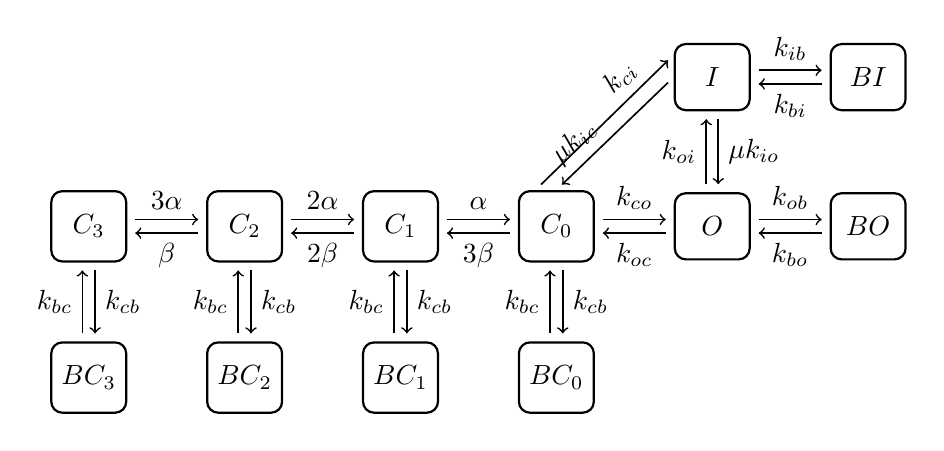
\begin{tikzpicture}[
   font=\sffamily,
   every matrix/.style={ampersand replacement=\&,column sep=1cm,row sep=1cm},
   state/.style={draw,thick,rounded corners,inner sep=.3cm},
   to/.style={->,semithick,shorten >=0.1cm,shorten <=0.1cm},
   Q/.style={->,semithick,sloped,below, above,pos=0.720000,shorten >=0.1cm,shorten <=0.1cm},  
   %Q/.style={->,semithick,pos=0.60000,shorten >=0.1cm,shorten <=0.1cm},  
   every node/.style={auto}]
\matrix{
\&\&\&\&\node[state] (I) {\parbox{10pt}{\centerline{$I$}}};\&\node[state] (BI) {\parbox{10pt}{\centerline{$BI$}}};\\
\node[state] (C_{3}) {\parbox{10pt}{\centerline{$C_{3}$}}};\&\node[state] (C_{2}) {\parbox{10pt}{\centerline{$C_{2}$}}};\&\node[state] (C_{1}) {\parbox{10pt}{\centerline{$C_{1}$}}};\&\node[state] (C_{0}) {\parbox{10pt}{\centerline{$C_{0}$}}};\&\node[state] (O) {\parbox{10pt}{\centerline{$O$}}};\&\node[state] (BO) {\parbox{10pt}{\centerline{$BO$}}};\\
\node[state] (BC_{3}) {\parbox{10pt}{\centerline{$BC_{3}$}}};\&\node[state] (BC_{2}) {\parbox{10pt}{\centerline{$BC_{2}$}}};\&\node[state] (BC_{1}) {\parbox{10pt}{\centerline{$BC_{1}$}}};\&\node[state] (BC_{0}) {\parbox{10pt}{\centerline{$BC_{0}$}}};\&\&\\
};
\draw[to]  (O.100) to node {$k_{oi}$} (I.260);
\draw[to]  (O.190) to node {$k_{oc}$} (C_{0}.350);
\draw[to]  (O.10) to node {$k_{ob}$} (BO.170);
\draw[to]  (I.280) to node {$\mu k_{io}$} (O.80);
\draw[Q]  (I.180) to node {$\mu k_{ic}$} (C_{0}.90);
\draw[Q]  (C_{0}.120) to node {$k_{ci}$} (I.150);
\draw[to]  (I.10) to node {$k_{ib}$} (BI.170);
\draw[to]  (C_{0}.10) to node {$k_{co}$} (O.170);
\draw[to]  (C_{0}.190) to node {$3\beta$} (C_{1}.350);
\draw[to]  (C_{0}.280) to node {$k_{cb}$} (BC_{0}.80);
\draw[to]  (C_{1}.10) to node {$\alpha$} (C_{0}.170);
\draw[to]  (C_{1}.190) to node {$2\beta$} (C_{2}.350);
\draw[to]  (C_{1}.280) to node {$k_{cb}$} (BC_{1}.80);
\draw[to]  (C_{2}.10) to node {$2\alpha$} (C_{1}.170);
\draw[to]  (C_{2}.190) to node {$\beta$} (C_{3}.350);
\draw[to]  (C_{2}.280) to node {$k_{cb}$} (BC_{2}.80);
\draw[to]  (C_{3}.10) to node {$3\alpha$} (C_{2}.170);
\draw[to]  (C_{3}.280) to node {$k_{cb}$} (BC_{3}.80);
\draw[to]  (BO.190) to node {$k_{bo}$} (O.350);
\draw[to]  (BI.190) to node {$k_{bi}$} (I.350);
\draw[to]  (BC_{0}.100) to node {$k_{bc}$} (C_{0}.260);
\draw[to]  (BC_{1}.100) to node {$k_{bc}$} (C_{1}.260);
\draw[to]  (BC_{2}.100) to node {$k_{bc}$} (C_{2}.260);
\draw[to]  (BC_{3}.100) to node {$k_{bc}$} (C_{3}.260);
\end{tikzpicture}
\end{center}
\caption{Markov model for a theoretical drug of the sodium channel. The model
consists of the usual states $O,I,C_{0},C_{1},C_{2}$, and $C_{3}$ and the blocked
states $BO,BI,BC_{0},BC_{1},BC_{2}$, and $BC_{3}$.}%
\label{mtreadr}%
\end{figure}




\subsection{Numerical experiments using the blocker of the inactivated state}

We have seen that a blocker of the inactivated state is a promising
candidate for repairing the mutation described in Figure \ref{mtreac}. The drug
is characterized by $\left(  \ref{drg_inac}\right)  $, so we have%
\begin{equation}
k_{ib}=\delta_{i}k_{bi}=\left(  \mu-1\right)  k_{bi} \label{kbi10}
\end{equation}
and the parameter $k_{bi}$ remains to be determined. In Table \ref{kbi_stat}, we show that the
blocker is more efficient the larger $k_{bi}$ is. In fact, the blocker is able to
repair all the relevant statistical properties of the solution. The statistical properties
presented in the table are introduced in Section \ref{statistics} on page \pageref{statistics}.


In Figure \ref{NaM/pdf_drug.pdf}, we show the open state probability density functions of the
wild type, the mutant, and the drugged version of the mutant. Again, we see
that the drug completely repairs the open state probability density function.

\fig{NaM/pdf_drug.pdf}{The open probability density function for the wild type
(WT) case and the mutant (MT) case using the mutation severity index $\mu=30$
and, finally, the mutant case with the drug given by (\ref{kbi10}) with 
$k_{bi} = 0.001\text{ ms}^{-1}$. A small value of $k_{bi}$ was used to
see a difference between the drugged case and the WT case.}

\begin{table}  \begin{center}
\begin{tabular}{|r|r|r|r|} \hline
$k_{bi}$ & $\pi_o\times 10^3 $ & $E_o$ & $\sigma_o$ \\ \hline
WT & 0.067 & -50.794 & 46.828 \\ \hline
MT & 1.534 & 12.991 & 26.831 \\ \hline
$10^{-6}$ & 1.341 & 12.940 & 26.913 \\ \hline
$10^{-5}$ & 1.180 & 12.487 & 27.634 \\ \hline
$10^{-4}$ & 0.556 & 8.240 & 33.343 \\ \hline
$10^{-3}$ & 0.135 & -16.903 & 49.326 \\ \hline
0.01 & 0.070 & -47.563 & 48.205 \\ \hline
0.1 & 0.067 & -50.729 & 46.869 \\ \hline
1 & 0.067 & -50.791 & 46.830 \\ \hline
\end{tabular} \end{center}
\caption{The open probability, $\pi_o$, the expected value of the transmembrane potential, $E_o$, and the
standard deviation, $\sigma_o$, for increasing values of $k_{bi}$. For large values of $k_{bi}$, the statistical properties 
of the mutant are completely repaired by the drug. 
}
\label{kbi_stat}
\end{table}

\subsection{The late sodium current is removed by the inactivated state blocker}


In Figure \ref{NaM/mc.pdf} above, we demonstrated, using Monte Carlo simulations, that the
mutation under consideration leads to a significant late sodium current
comparable to the current observed in experiments. By using the drug described
in $\left(  \ref{drg_inac}\right) $ with $k_{bi}=0.01 \text{ ms}^{-1},$ we see that the late
current more or less completely disappears (see Figure \ref{NaM/mc_drug}).

\fig{NaM/mc_drug}{The sodium current for the wild type (WT) and the mutant (MT)
with the mutation severity index $\mu=30$. The drug given by (\ref{kbi10}) with $k_{bi} = 0.01 \text{ ms}^{-1}$
almost completely removes the late sodium current.}


\section{Notes}

\begin{enumerate}
\item The basic structure of the Markov model in Figure \ref{wtreac} is taken 
from Patlak \cite{Patlak1991}, who discusses and evaluates several possible models in relation to experimental data.

\item Modeling the effects of a drug on the sodium channel is motivated by
the paper of Clancy et al. \cite{Clancy2007}.


\end{enumerate}



%
%
%


\chapter{Mutations affecting the mean open time \label{mot_chapter}}

In the simplest case of Markov models of the form
\begin{equation}
C\underset{k_{co}}{\overset{k_{oc}}{\leftrightarrows}}O, \label{mot_markov}%
\end{equation}
we have studied mutations leading to an increased open probability by increasing
the rate from closed (C) to open (O), given by $k_{co}$. We refer to these as 
CO-mutations and for such mutations we
have successfully derived closed state blockers represented as%
\begin{equation}
B\underset{k_{bc}}{\overset{k_{cb}}{\leftrightarrows}}C\underset{\mu
k_{co}}{\overset{k_{oc}}{\leftrightarrows}}O, \label{mot_cl}%
\end{equation}
where $\mu\geqslant1$ is the mutation severity index and $\mu=1$
represents the wild type. These blockers can completely repair the equilibrium
open probability of the mutant by adjusting the ``on rate'' divided by the
``off rate'' of the drug given by
\[
\delta_{c}=\frac{k_{cb}}{k_{bc}}
\]
(see, e.g., page \pageref{d_c}). The remaining degree of freedom can be found
using probability density systems and the resulting drugs have been proven to
work exceptionally well in theoretical computations.

There is, however, another way of modeling increased equilibrium open
probability. Rather than increasing the rate from C to O, we can reduce the
rate from O to C:%
\begin{equation}
C\underset{k_{co}}{\overset{k_{oc}/\mu}{\leftrightarrows}}O,
\end{equation}
where again $\mu\geqslant1$ is referred to as the mutation severity index. 
This type of mutation is referred to as an OC-mutation and the
equilibrium open probability for this Markov model is given by%
\[
o=\frac{1}{1+\frac{k_{oc}/\mu}{k_{co}}},%
\]
which clearly increases for increasing values of $\mu.$ Formally, we can carry out
the same math to devise a closed state drug that completely repairs the
equilibrium open probability of the mutant; however, when this drug is put into the
probability density system to determine the remaining degree of
freedom of the drug, we quickly observe that the task is impossible and the
theoretical drug does not provide significant improvement.

The core difficulty here is that a CO-mutation does not
change the mean open time of the channel. A closed state blocker is therefore
well suited because such a blocker does not affect the mean open time. 
However, for an OC-mutation,
an increased mean open time is part of the problem and a closed state blocker
is not the solution, simply because it cannot affect the mean open time. Rather, an open state blocker must be used.

In this chapter, we will explain the notion of mean open time and study
mutations that lead to an increased open probability \textit{and} an increased mean
open time. We will show that open state blockers are optimal for such mutations.

\section{The mean open time}

Let us briefly recall the interpretation of the Markov model
\[
C\underset{k_{co}}{\overset{k_{oc}}{\leftrightarrows}}O.
\]
This scheme means that if the channel is closed (C), the probability of
changing the state from closed to open (O) in a small time interval $\Delta t$ is
given by $k_{co}\Delta t.$ Clearly, this interpretation only holds for short
time intervals, since the probability cannot exceed one. Note also that if the
rate $k_{co}$ increases, this leads to an increased probability of moving from C
to O during the time step $\Delta t.$ Similarly, $k_{oc}\Delta t$ denotes the
probability of moving from the open state to the closed state in the time step
$\Delta t.$

Suppose that the channel is open at time $t=0.$ The probability that the
channel remains open after a short time step $\Delta t$ is given by%
\[
p_{1}=1-k_{oc}\Delta t.
\]
If we take another time step, the probability that the channel is still open
at time $t=2\Delta t$ is given by%
\[
p_{2}=p_{1}\left(  1-k_{oc}\Delta t\right)  =\left(  1-k_{oc}\Delta t\right)
^{2}%
\]
and so on. At time $t=n\Delta t,$ the probability of the channel still being
open is given by%
\[
p_{n}=\left(  1-k_{oc}\Delta t\right)  ^{n}.
\]
If we now introduce time given by%
\[
t=n\Delta t,
\]
we have%
\[
\left(  1-k_{oc}\Delta t\right)  ^{n}=\left(  1-k_{oc}\Delta t\right)
^{\frac{t}{\Delta t}}.%
\]
The probability of closing a channel that is in the open state during a
time step is given by $\Delta tk_{oc}$ and therefore the probability of
closing a channel that has remained open for $n$ time steps is given by%
\[
\Delta tk_{oc}\left(  1-k_{oc}\Delta t\right)  ^{\frac{t}{\Delta t}}.
\]
The expected open time is therefore given by%
\[
\sum_{n=1}^{\infty}n\Delta t\left(  1-k_{oc}\Delta t\right)  ^{\frac{t}{\Delta
t}}\Delta tk_{oc}.
\]
If we go to the limit of $\Delta t\rightarrow0$ in this expression, we find
that%
\[
\sum_{n=1}^{\infty}n\Delta t\left(  1-k_{oc}\Delta t\right)  ^{\frac{t}{\Delta
t}}\Delta tk_{oc}\overset{\Delta t\rightarrow0}{\longrightarrow}\int%
_{0}^{\infty}tk_{oc}e^{-k_{oc}t}dt=\frac{1}{k_{oc}}%
\]
and therefore we have found that the mean open time is given by%
\begin{equation}
\tau_{o}=\frac{1}{k_{oc}}. \label{tau_o}%
\end{equation}


\subsection{Mean open time for more than one open state\label{mot_many}}


We have seen that the mean open time for a Markov model of the form
\[
C\underset{k_{co}}{\overset{k_{oc}}{\leftrightarrows}}O
\]
is given by
\begin{equation}
\tau_{o}=\frac{1}{k_{oc}}. %
\end{equation}
It is straightforward to extend the argument above to see that, for a Markov
model of the form 
\[
C\underset{k_{co}}{\overset{k_{oc}}{\leftrightarrows}}O\underset{k_{ob}}{\overset{k_{bo}}{\leftrightarrows}}B,
\]
the mean open time is given by
\begin{equation}
\tau_{o}=\frac{1}{k_{oc}+k_{ob}}. %
\end{equation}
But what happens if there is more than one open state? This situation
will become relevant below, where we consider models including a burst mode.
The models contain at least two open states. To understand the mean
open time in the presence of more than one open state, we consider the
generic extension illustrated in Figure \ref{o2}.

%
\begin{figure}[ptb]
\begin{center}
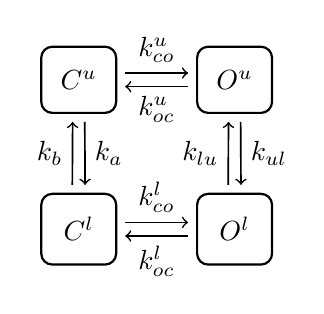
\begin{tikzpicture}[
   font=\sffamily,
   every matrix/.style={ampersand replacement=\&,column sep=1cm,row sep=1cm},
   state/.style={draw,thick,rounded corners,inner sep=.3cm},
   to/.style={->,semithick,shorten >=0.1cm,shorten <=0.1cm},
   Q/.style={->,semithick,sloped,pos=0.700000,shorten >=0.1cm,shorten <=0.1cm}, 
   every node/.style={auto}]
\matrix{
\node[state] (C^{u}) {\parbox{10pt}{\centerline{$C^{u}$}}};\&\node[state] (O^{u}) {\parbox{10pt}{\centerline{$O^{u}$}}};\\
\node[state] (C^{l}) {\parbox{10pt}{\centerline{$C^{l}$}}};\&\node[state] (O^{l}) {\parbox{10pt}{\centerline{$O^{l}$}}};\\
};
\draw[to]  (C^{u}.10) to node {$k_{co}^{u}$} (O^{u}.170);
\draw[to]  (C^{u}.280) to node {$k_{a}$} (C^{l}.80);
\draw[to]  (O^{u}.190) to node {$k_{oc}^{u}$} (C^{u}.350);
\draw[to]  (O^{u}.280) to node {$k_{ul}$} (O^{l}.80);
\draw[to]  (C^{l}.100) to node {$k_{b}$} (C^{u}.260);
\draw[to]  (C^{l}.10) to node {$k_{co}^{l}$} (O^{l}.170);
\draw[to]  (O^{l}.100) to node {$k_{lu}$} (O^{u}.260);
\draw[to]  (O^{l}.190) to node {$k_{oc}^{l}$} (C^{l}.350);
\end{tikzpicture}
\end{center}
\caption{Markov model with two open states ($O^{u}$, $O^{l}$) and two closed states ($C^{u}$, $C^{l}$).}%
\label{o2}%
\end{figure}
Assuming that the rates are set according to the principle of detailed balance,
 we have
\[k_{ul}o_{u}=k_{lu}o_{l}, \]
where $o_{u}$ and $o_{l}$ are the probabilities of being in the states 
$O^{u}$ or $O^{l}$, respectively, and $u$ and $l$ represent the upper and lower states,
respectively. 

As for the derivation above, we assume that the channel is open and
our task is to figure out how long we can expect the channel to remain open. We
know that, initially, the channel is either in the state $O^{u}$ or
$O^{l}$. Let us define $q_u$ and $q_l$ to be the conditional 
probabilities of being in the upper and lower open states, given that the channel is open. For the upper state we write
\[ q_u = P(S=O_u | (S={O_u} \mbox{\ or\ } S={O_l})), \]
where $S=X$ means that the channel is in state $X$.
Since
\[ P(A|B) = P(A \mbox{\ and\ } B)/P(B) \]
 and, in our case, since ($A$ and $B$) = $A$, we obtain
\[ q_u = P(S=O_u)/P(S={O_u} \mbox{\ or\ } S={O_l}) = \frac{o_u}{o_u+o_l} \]
and similarly for the lower state; with
\[ q_l = P(S=O_l | (S={O_u} \mbox{\ or\ } S={O_l})), \]
we obtain
\[ q_l  = \frac{o_l}{o_u+o_l}.\]
It follows that $q_u + q_l = 1$ and that

\[
q_{u}=\frac{k_{lu}}{k_{ul}+k_{lu}}%
\]
and%
\[
q_{l}=\frac{k_{ul}}{k_{ul}+k_{lu}}.
\]
The probability of remaining in the open states in the first time step is now given
by%
\begin{align*}
p_{1}  & =\left(  1-\Delta tk_{oc}^{u}\right)  q_{u}+\left(  1-\Delta
tk_{oc}^{l}\right)  q_{l}\\
& =1-\Delta t\left(  \frac{k_{oc}^{u}k_{lu}+k_{oc}^{l}k_{ul}}{k_{ul}+k_{lu}%
}\right)  
\end{align*}
and thus, by following the steps above, we find that%
\[
p_{n}=\left(  1-\Delta tK\right)  ^{n},
\]
where%
\[
K=\frac{k_{oc}^{u}k_{lu}+k_{oc}^{l}k_{ul}}{k_{ul}+k_{lu}}.
\]
The probability of closing a channel that is in one of the open states during
a time step is given by%
\[
\Delta tk_{oc}^{u}q_{u}+\Delta tk_{oc}^{l}q_{l}=\Delta tK
\]
and, therefore, the probability of closing a channel in a time step that has
remained open for $n$ time steps is given by%
\[
\Delta tK\left(  1-\Delta tK\right)^{n}.%
\]
We find  that the expected mean open time is given by%
\begin{equation}
\tau_{o}=\frac{1}{K}=\frac{k_{ul}+k_{lu}}{k_{oc}^{u}k_{lu}+k_{oc}^{l}k_{ul}}. \label{tau_oo}
\end{equation}

\subsubsection{Special cases}

It is interesting to consider the formula  for the mean open time given 
by $(\ref{tau_oo})$ in two special cases. First, we assume that 
$k^u_{oc}=k^l_{oc}$  and we let $k_{oc}$ denote this common value. Then, by $(\ref{tau_oo})$, we have 
\begin{equation*}
\tau_{o}=\frac{1}{k_{oc}}
\end{equation*}
which is the same as we found for the two-state scheme above. Next consider the case of $k_{ul}=k_{lu}$  (and 
$k^u_{oc}\not=k^l_{oc}$). By $(\ref{tau_oo})$, we find 
\begin{equation}
\tau_{o}=\frac{1}{(k_{oc}^{u}+k_{oc}^{u})/2}. \label{tau_ooo}
\end{equation}


\section{Numerical experiments}

It is useful to have a look at the mean open time computed in specific
numerical experiments to determine how well it is represented by the theoretical
value derived above. Similarly, it is useful to consider how well the
theoretical equilibrium open probability represents the data we observe in
actual computations. In this section, we will present experiments that
hopefully clarify these matters.

\subsection{Mean open time and equilibrium open probability: Theoretical
values versus sample mean values}

Let us illustrate the result above by a few numerical experiments. We start by
considering the Markov model%
\[
C\underset{k_{co}}{\overset{k_{oc}}{\leftrightarrows}}O,
\]
where we set $k_{co}=1$ ms$^{-1}$ and we let
\[
k_{oc}=\frac{1}{m}\text{ms}^{-1}%
\]
for $m=1,...,100.$ For every value of $k_{oc},$ we run a simulation using the
Markov model for $T=10^{4}$ ms. The time instances when the channel changes
state are stored in the sequence $\left\{  t_{i}\right\}  _{i=0}^{N}$ and the
mean open time observed in the simulation is given by\footnote{The
index $s$ here is used to indicate {\it sample}, since these are values for a
specific computation and not the theoretical value computed above.}
\[
\tau_{o,s}=\frac{2}{N}\sum_{i}\left(  t_{i}-t_{i-1}\right)  _{o},%
\]
where
\[
\left(  t_{i}-t_{i-1}\right)  _{o}=\left\{
\begin{array}
[c]{ll}%
t_{i}-t_{i-1}\text{ } & \text{if the channel is open in this interval,}\\
0\text{ } & \text{if the channel is closed in this interval.}%
\end{array}
\text{ }\right.
\]
With this notation we can also define the sample open probability by%
\[
o_{s}=\frac{1}{T}\sum_{i}\left(  t_{i}-t_{i-1}\right)  _{o}.
\]
In Figure  \ref{MOT/mot.pdf} (left panel), we plot the sample mean open time 
$\tau_{o,s}$ and the theoretical mean open time given by%
\begin{equation}
\tau_{o}=\frac{1}{k_{oc}} \label{mot2}%
\end{equation}
as functions of $k_{oc}.$ We also plot (right panel) the sample open
probability $o_{s}$ and the theoretical equilibrium probability given by%
\begin{equation}
o=\frac{1}{1+\frac{k_{oc}}{k_{co}}}. \label{mot3}%
\end{equation}
In both plots, we see that the mean values computed in the simulations are
quite close to the theoretical values. If we increase the simulation time $T,$
these graphs converge toward the same value.

\fig{MOT/mot.pdf}{Mean open time (left) and open probability (right), with $k_{oc}=1/m$ ms$^{-1}$ and $k_{co}=1$ ms$^{-1}$. The sample
values (dashed lines) correspond well with the theoretical values (solid line).}


\subsection{The closed to open rate $k_{co}$ does not affect the mean open
time}

We have seen that, theoretically, according to $\left(  \ref{mot2}\right)  ,$
the mean open time $\tau_{o}$ is independent of the closed to open rate
$k_{co},$ but the open probability is affected as stated in $\left(
\ref{mot3}\right)  .$ This is illustrated in Figure \ref{MOT/mct.pdf}, where we use
$k_{oc}=1$ ms$^{-1}$ and $k_{co}=1/m$ ms$^{-1}$ 
and plot the mean open time (left panel) and the open
probability (right panel) as functions of $m.$

\fig{MOT/mct.pdf}{Mean open time (left) and open probability (right) with $k_{co}=1/m$ ms$^{-1}$ and $k_{oc}=1$ ms$^{-1}$. The mean open
time is not affected by changes in $k_{co}$. The sample values correspond well to 
the theoretical values.}


\subsection{The mean open time in the presence of two open states}
In Figure \ref{MOT/burst_mot.pdf}, we show the sample mean open time and the theoretical mean open time given by 
\begin{equation}
\tau_{o}=\frac{1}{K}=\frac{k_{ul}+k_{lu}}{k_{oc}^{u}k_{lu}+k_{oc}^{l}k_{ul}} 
\end{equation}
for the Markov model in Figure \ref{o2}. In the computations, we have used $k^l_{oc} = 1$ ms$^{-1}$, $k^u_{oc} = 10$ ms$^{-1}$, and $k_{lu}  = 0.001$ ms$^{-1}$ and $k_{ul}$ varies. The other parameters of the model do not affect the result, as long as detailed balance holds.
\fig{MOT/burst_mot.pdf}{Mean open time for a Markov model with two open states.}


\subsection[Changing MOT affects the dynamics of the transmembrane potential]{Changing the mean open time affects the dynamics of the transmembrane potential}
%\K{zzz For meg virker det som at parametrene som i de tidligere kapitlene 
%har blitt kalt for $V_{Na}$ og lignende n\r{a} blir kalt for $E_{Na}$ og lignende.
%Hvis det er tilfellet, er det greit med to forskjellige notasjoner eller
%burde det brukes den samme notasjonen? I kapittel 12 ble de samme 
%parameterverdiene brukt, men da ble $g_{K}$ og $E_{K}$ kalt for $g_{L}$ og $V_{L}$.
%Er det meningen at dette skal v\ae re det samme eksempelet eller er dette et
%annet eksempel?}
%\A{I have changed all back to $V_{Na}$ and $V_{K}$.}
We consider the stochastic model of the transmembrane potential given by
\begin{equation}
v_{t}=g_{K}(V_{K}-v)+\gamma g_{Na}(V_{Na}-v) \label{mot_s_1},%
\end{equation}
where $\gamma$ is a stochastic variable governed by the two-state Markov
model
\[
C\underset{k_{co}}{\overset{k_{oc}}{\leftrightarrows}}O.
\]
We use the parameters%
\begin{align}
g_{K}  &  =\frac{1}{10}\text{ ms}^{-1},\text{ }g_{Na}=1\text{ ms}%
^{-1}, \label{mmm_dta}\\
V_{K} &  =-85\text{ mV, }V_{Na}=45\text{ mV,}\nonumber
\end{align}
and compute solutions using the standard scheme
\begin{equation}
v_{n+1}=v_{n}-\Delta t\left(  g_{K}\left(  v_{n}-V_{K}\right)  +\gamma
_{n}g_{Na}(v_{n}-V_{Na}\right)  ), \label{mot_vs}%
\end{equation}
where the time step is assumed to satisfy the condition%
\begin{equation}
\Delta t<\frac{1}{g_{K}+g_{Na}}.
\end{equation}
Under this condition, we have seen above that, for solutions computed by
$\left(  \ref{mot_s_1}\right),  $ an invariant region is given by
\begin{equation}
\Omega=\left(  V_{K},V_{+}\right)  ,
\end{equation}
where%
\[
V_{+}=\frac{g_{K}V_{K}+g_{Na}V_{Na}}{g_{K}+g_{Na}}.
\]
In Figure \ref{MOT/time.pdf}, we show numerical solutions of $\left(  \ref{mot_s_1}\right)  $
for
\[
k_{oc}=k_{co}=0.1\text{ ms}^{-1},1\text{ ms}^{-1}, 10\text{ ms}^{-1}, 100 \text{ ms}^{-1}.
\]
According to the considerations above, the equilibrium open probability is
given by%
\[
o=\frac{1}{1+\frac{k_{oc}}{k_{co}}},%
\]
which is constant for the four parameter sets used in Figure \ref{MOT/time.pdf}. The mean
open time, however, varies with $k_{oc}$ as%
\[
\tau_{o}=\frac{1}{k_{oc}}.
\]
For the cases studied in Figure \ref{MOT/time.pdf}, the mean open times are 
10 ms, 1 ms, 1/10 ms, and 1/100 ms and we observe that the reduced mean open time greatly 
reduces the variations of the transmembrane potential.

\fig[0.95]{MOT/time.pdf}{Simulations based on the numerical scheme (\ref{mot_vs}) with 
changing reaction rates for the Markov model.
From top to bottom, $k_{oc}=k_{co}=0.1\text{ ms}^{-1}$, $1 \text{ ms}^{-1}$, $10\text{ ms}^{-1}$, and $100 \text{ ms}^{-1}.$ 
Since $k_{oc}=k_{co}$ for all values, the open probability
is kept constant but the mean open time given by $1/k_{oc}$ is decreasing from top 
to bottom. }


\section[Changing MOT affects the PDFs]{Changing the mean open time affects the probability density functions}

The stationary version of the probability density system governing the states
of the Markov model%
\[
C\underset{k_{co}}{\overset{k_{oc}}{\leftrightarrows}}O
\]
is given by%

\begin{align}
\frac{\partial}{\partial v}\left(  a_{o}\rho_{o}\right)   &  =k_{co}\rho
_{c}-k_{oc}\rho_{o},\label{vpdf_mot}\\
\frac{\partial}{\partial v}\left(  a_{c}\rho_{c}\right)   &  =k_{oc}\rho
_{o}-k_{co}\rho_{c},\nonumber
\end{align}
where 
\begin{align}
a_{o}  &  =g_{K}(V_{K}-v)+g_{Na}(V_{Na}-v),\label{vflux_mot}\\
a_{c}  &  =g_{K}(V_{K}-v).\nonumber
\end{align}
The analytical solution of this problem is given by%

\begin{align*}
\rho_{o}(v)  &  =Kg_{K}(V_{+}-v)^{\frac{k_{oc}}{g}-1}(v-V_{K})^{\frac{k_{co}%
}{g_{K}}},\\
\rho_{c}(v)  &  =Kg(V_{+}-v)^{\frac{k_{oc}}{g}}(v-V_{K})^{\frac{k_{co}}{g_{K}}-1},%
\end{align*}
%\K{zzz Det skal vel egentlig st\r{a} v der det st\r{a}r x i disse uttrykkene?
%Og blir det ikke $(v-V_{K})$ i stedet for $(V_{K}-v)$ 
%siden vi antar $v \in (V_{K},V_{+})$?}\A{ Changed according to K.}
where
\[
g=g_{Na}+g_{K}\text{, }V_{+}=\frac{g_{Na}V_{Na}+g_{K}V_{K}}{g_{Na}+g_{K}}%
\]
%\K{zzz Denne E-en ble kalt for $V_{+}$ i forrige seksjon.}\A{ Changed according to K.}
and $K$ is chosen such that%
\[
\int_{V_{K}}^{V_{+}}\rho_{o}+\rho_{c}=1,
\]
which is given by
\[
1/K=\frac{k_{co}+k_{oc}}{a+b} (V_+-V_K)^{(a+b)} B(a,b),
\]
with $a = k_{co}/g_{K}, b = k_{oc}/g$, and $B(a,b) =\Gamma(a)\Gamma(b)/\Gamma(a+b)$.
%\K{zzz Burde det st\r{a} $V_{K}$ i stedet for $V_{-}$ i uttrykket slik at det henger mer sammen med det over?}


In Figure \ref{MOT/pdf.pdf}, we show the open probability density function for the data given
in $\left( \ref{mmm_dta}\right)  $ with
\[
k_{oc}=k_{co}=0.1 \text{ ms}^{-1},1\text{ ms}^{-1},10\text{ ms}^{-1},100 \text{ ms}^{-1}.
\]
Again, we recall that as $k_{oc}$ increases, the mean open time
decreases and we observe in the figure that the probability density function
becomes narrower.
%\K{zzz stoppet her}

\fig{MOT/pdf.pdf}{The open probability density function $\rho_o$ (solid line) and closed
 probability density function $\rho_c$ depend on the mean open time given by $1/k_{oc}$. In the figures,
 we have used $k=k_{oc}=k_{co}.$}

\bigskip

\begin{comment}
\subsection{The limit of the zero mean open time}

In Figure \ref{MOT/pdf.pdf}, we observed that as $k_{oc}$ and $k_{co}$ increase, the open
probability density function becomes increasingly narrow and it is tempting to
understand where this ends. Let $k=k_{oc}=k_{co}$ and consider the probability
density system%
\begin{align}
\frac{1}{k}\frac{\partial}{\partial v}\left(  a_{o}\rho_{o}\right)   &
=\rho_{c}-\rho_{o},\label{mot_k}\\
\frac{1}{k}\frac{\partial}{\partial v}\left(  a_{c}\rho_{c}\right)   &
=\rho_{o}-\rho_{c}.\nonumber
\end{align}
In the limit of $k\longrightarrow\infty,$ the mean open time
\[
\tau_{o}=\frac{1}{k_{oc}}=\frac{1}{k}\longrightarrow0
\]
and, by (\ref{mot_k}), we have
\[
\rho_{c}=\rho_{o}.
\]
By adding the equations, we obtain (for any value of $k$)%
\[
\frac{\partial}{\partial v}\left(  a_{o}\rho_{o}+a_{c}\rho_{c}\right)  =0
\]
and with $\rho_{o}=\rho_{c},$ this yields%
\[
\frac{\partial}{\partial v}\left(  \left(  a_{o}+a_{c}\right)  \rho
_{o}\right)  =0.
\]
Since $\rho_{o}=0$ for sufficiently large values of $\left\vert v\right\vert
,$ we find that%
\begin{equation}
\left(  a_{o}+a_{c}\right)  \rho_{o}=0 \label{0}%
\end{equation}
for almost all\footnote{This means {\sl almost all} in this sense: \url{http://en.wikipedia.org/wiki/Almost_all}.} $v$. Since
 $\rho_{o}=\rho_{c},$ we have%
\[
\int\rho_{o}dv=\frac{1}{2}%
\]
and thus $\rho_{o}=\frac{1}{2}\delta\left(  v-v_{\ast}\right)  , $ where
$\delta$ is the Dirac delta function. In general, we have%
\[
\int f(v)\delta\left(  v-v_{\ast}\right)  dv=f\left(  v_{\ast}\right)
\]
and, therefore, by (\ref{0}), we must have%
\[
\left(  a_{o}+a_{c}\right)  \left(  v_{\ast}\right)  =\frac{1}{2}\int\left(
a_{o}+a_{c}\right)  \left(  v\right)  \delta\left(  v-v_{\ast}\right)
dv=0.
\]
By using the definitions $\left(  \ref{vflux_mot}\right)  $, we obtain%
\[
2g_{K}(V_{K}-v_{\ast})+g_{Na}(V_{Na}-v_{\ast})=0
\]
and therefore%
\[
v_{\ast}=\frac{2g_{K}V_{K}+g_{Na}V_{Na}}{2g_{K}+g_{Na}}.
\]
In Figure \ref{MOT/pdf.pdf} we show the open and closed probability density functions
defined by the system $\left(  \ref{mot_k}\right)  .$ We observe that as $k$
increases, the functions converges and the distributions center around
$v_{\ast}=23.33$ mV. In these computations we have used the parameters defined in (\ref{mmm_dta}).

{\bf xxx Glenn: Kan du legge inn stoerre verdier av $k$ slik at vi ser at 
peak-verdier  konvergerer mot $v^*$?}
\G{Updated parameter value in text, peak should be at $v_{\ast}=23.33.$, so the plots are OK as is I guess.}

\end{comment}


\section{Theoretical drugs for OC-mutations}

We have seen earlier that when mutations increase the open probability by
increasing the reaction rate from C to O $(k_{co}),$ the effect of the
mutation can be completely repaired by using an optimal closed state blocker.
Now we are interested in a mutation that increases the open probability by reducing
the reaction rate from O to C $\left(  k_{oc}\right).$ Such a mutation
increases both the open probability and  the mean open time
and we will observe that a closed state blocker is unable to repair the effect
of such a mutation.

We consider the two-state Markov model
\begin{equation}
C\underset{k_{co}}{\overset{k_{oc}/\mu}{\leftrightarrows}}O, \label{mmm0}%
\end{equation}
where $\mu\geqslant1$ is the mutation severity index; as usual, $\mu=1$ denotes
the wild type. Recall that the equilibrium open probability is given by%
\[
o=\frac{1}{1+\frac{k_{oc}}{\mu k_{co}}}%
\]
and the mean open time is given by%
\[
\tau_{o}=\frac{\mu}{k_{oc}},%
\]
so the mutation clearly increases both the open probability and the mean open time.

\bigskip

\subsection{The theoretical closed state blocker does not work for the OC-mutation}

Let us start by considering a closed state blocker of the form%
\begin{equation}
B\underset{k_{bc}}{\overset{k_{cb}}{\leftrightarrows}}C\underset{k_{co}}{\overset{k_{oc}/\mu}{\leftrightarrows}}O. \label{mmm1}%
\end{equation}
%\K{zzz Burde man i denne Markov-modellen heller ta med at vi deler $k_{oc}$ 
%p\r{a} $\mu$?}
% A: ja; fixet
We find that the equilibrium open probability of the mutant in the presence of the
closed state blocker is given by%
\[
o=\frac{1}{1+\frac{k_{oc}}{k_{co}}\frac{1+\delta_{c}}{\mu}},%
\]
where%
\[
\delta_{c}=\frac{k_{cb}}{k_{bc}}.
\]
Since the wild type equilibrium open probability is given by%
\[
o=\frac{1}{1+\frac{k_{oc}}{k_{co}}},%
\]
the drug will repair the open probability, provided that%
\[
\frac{1+\delta_{c}}{\mu}=1
\]
and therefore the drug must satisfy the usual condition%
\[
\delta_{c}=\mu-1.
\]
A drug satisfying this condition will completely repair the equilibrium open
probability and that is, of course, good, but it is not enough. Since the
mutation represented by $\left(  \ref{mmm0}\right)  $ also affects the mean
open time, a drug of the form $\left(  \ref{mmm1}\right)  $ cannot repair that
effect of the mutation. To see this, we consider the probability
density system defined by%
\begin{align}
\frac{\partial}{\partial v}\left(  a_{o}\rho_{o}\right)   &  =k_{co}\rho
_{c}-\frac{1}{\mu}k_{oc}\rho_{o},\nonumber\\
\frac{\partial}{\partial v}\left(  a_{c}\rho_{c}\right)   &  =\frac{1}{\mu}k_{oc}\rho
_{o}-\left(  k_{co}+\left(  \mu-1\right)  k_{bc}\right)  \rho_{c}+k_{bc}%
\rho_{b},\label{mmm3}\\
\frac{\partial}{\partial v}\left(  a_{c}\rho_{b}\right)   &  =\left(
\mu-1\right)  k_{bc}\rho_{c}-k_{bc}\rho_{b},\nonumber
\end{align}
%\K{zzz Skal man ikke i disse ligningene dele $k_{oc}$ p\r{a} $\mu$?}
where, as usual, $\rho_{o},\rho_{c},$ and $\rho_{b}$ denote the probability
density functions of the open (O), closed (C), and blocked (B) states,
respectively, and where the fluxes are defined by $\left(  \ref{vflux_mot}%
\right)  $. In Figure \ref{MOT/cb.pdf}, we compare the open probability density computed by
solving the system $\left(  \ref{mmm3}\right)  $ with the open probability
density of the wild type. The wild type probability density functions are
given by%

\begin{align}
\frac{\partial}{\partial v}\left(  a_{o}\rho_{o}\right)   &  =k_{co}\rho
_{c}-k_{oc}\rho_{o},\label{mmm4}\\
\frac{\partial}{\partial v}\left(  a_{c}\rho_{c}\right)   &  =k_{oc}\rho
_{o}-k_{co}\rho_{c},\nonumber
\end{align}
and the probability density functions of the mutant case are given by
\begin{align}
\frac{\partial}{\partial v}\left(  a_{o}\rho_{o}\right)   &  =k_{co}\rho
_{c}-\frac{1}{\mu}k_{oc}\rho_{o},\label{mutant44}\\
\frac{\partial}{\partial v}\left(  a_{c}\rho_{c}\right)   &  =\frac{1}{\mu}k_{oc}\rho
_{o}-k_{co}\rho_{c}.\nonumber
\end{align}
In the computations we have used the parameters given by $\left(
\ref{mmm_dta}\right)  $ and the rates%
\[
k_{co}=1\text{ ms}^{-1} \text{ and }k_{oc}=1\text{ ms}^{-1}.
\]
We use three values of the rates $k_{bc}$ and we observe that no parameter is
able to repair the open state probability density function of the mutation. In
Figure \ref{MOT/norm.pdf}, we show the norm of the difference between the open probability
density defined by $\left(  \ref{mmm3}\right)  $ and $\left(  \ref{mmm4}%
\right)  .$ The norm is defined by $\left(  \ref{norm}\right)  $ on page
\pageref{norm} and we see that no version of the closed state blocker defined 
by $\left(  \ref{mmm1}\right)  $ is able to repair the effect of the mutations
given by $\left(  \ref{mmm0}\right)  .$

\fig{MOT/cb.pdf}{The solid line represents the wild type solution and the dashed line represents the mutant. Various closed state drugs are applied, but none are able to repair the effect of the mutation.}

\fig{MOT/norm.pdf}{The norm of the difference between the wild type solution and the mutant after the drug is applied. 
The norm is defined by $\left(  \ref{norm}\right)  $ on page \pageref{norm}. We see that no value of the drug parameter 
$k_{bc}$ for the closed state blocker is able to repair the effect of the mutation.
}


\subsection{The theoretical open state blocker repairs the effect of the OC-mutation}

Next, we consider an open state blocker for the mutation leading to both an
increased open probability and an increased mean open time. The theoretical open 
state blocker can be written in the form%
\begin{equation}
C\underset{k_{co}}{\overset{k_{oc}/\mu}{\leftrightarrows}}O\underset{k_{ob}%
}{\overset{k_{bo}}{\leftrightarrows}}B, \label{mmob1}%
\end{equation}
where the parameters $k_{bo}$ and $k_{ob}$ define the theoretical drug. For this
Markov model, the equilibrium open probability is given by%
\[
o_{\mu}=\frac{1}{1+\frac{k_{oc}}{\mu k_{co}}+\frac{k_{ob}}{k_{bo}}}%
\]
and the mean open time is given by%
\[
\tau_{o,\mu}=\frac{1}{\frac{1}{\mu}k_{oc}+k_{ob}}.
\]
Since the associated wild type values are%
\[
o=\frac{1}{1+\frac{k_{oc}}{k_{co}}}%
\]
and
\[
\tau_{o}=\frac{1}{k_{oc}},
\]
we want to define the drug such that%
\[
1+\frac{k_{oc}}{\mu k_{co}}+\frac{k_{ob}}{k_{bo}}=1+\frac{k_{oc}}{k_{co}}%
\]
and%
\[
\frac{1}{\mu}k_{oc}+k_{ob}=k_{oc}.
\]
To satisfy these two requirements, we find that the drug must be given by
\begin{equation} \label{mot_o_drg}
\begin{aligned}
k_{ob}  &  =\frac{\mu-1}{\mu}k_{oc},\\
k_{bo}  &  =k_{co}.
\end{aligned}
\end{equation}

\subsection{The theoretical open state blocker is optimal}
We will show analytically that the open state blocker defined by (\ref{mmob1}) where the parameters are given by
(\ref{mot_o_drg}) is an optimal drug, in the sense that the effect of the mutation is completely repaired.
We start by observing that the probability density system associated with the Markov model  (\ref{mmob1}) is given by
\begin{align}
\frac{\partial}{\partial v}\left(  a_{o}\rho_{o}\right)   &  =k_{co}\rho
_{c}-(\mu^{-1}k_{oc}+k_{ob})\rho_{o}+k_{bo}\rho_{b},\nonumber\\
\frac{\partial}{\partial v}\left(  a_{c}\rho_{c}\right)   &  =\mu^{-1}%
k_{oc}\rho_{o}-k_{co}\rho_{c},\label{mm_dr_3}\\
\frac{\partial}{\partial v}\left(  a_{c}\rho_{b}\right)   &  =k_{ob}\rho
_{o}-k_{bo}\rho_{b}.\nonumber
\end{align}
If we insert the drug given by $\left(  \ref{mot_o_drg}\right)  $, we obtain the
system
\begin{align}
\frac{\partial}{\partial v}\left(  a_{o}\rho_{o}\right)   &  =k_{co}\rho
_{c}-k_{oc}\rho_{o}+k_{co}\rho_{b},\nonumber\\
\frac{\partial}{\partial v}\left(  a_{c}\rho_{c}\right)   &  =\mu^{-1}%
k_{oc}\rho_{o}-k_{co}\rho_{c},\label{mm_dr_o2}\\
\frac{\partial}{\partial v}\left(  a_{c}\rho_{b}\right)   &  =\left(
1-\mu^{-1}\right)  k_{oc}\rho_{o}-k_{co}\rho_{b}.\nonumber
\end{align}
We define%
\[
\bar{\rho}_{c}=\rho_{c}+\rho_{b}%
\]
and add the two latter equations of this system to find that $\rho_{o}$ and 
$\bar{\rho}_{c}$ solve the system%
\begin{align}
\frac{\partial}{\partial v}\left(  a_{o}\rho_{o}\right)   &  =k_{co}\bar{\rho
}_{c}-k_{oc}\rho_{o},\\
\frac{\partial}{\partial v}\left(  a_{c}\bar{\rho}_{c}\right)   &  =k_{oc}%
\rho_{o}-k_{co}\bar{\rho}_{c},\nonumber
\end{align}
which coincides with the system defining the wild type probability density
functions (see $\left(  \ref{mmm4}\right)  $ above). We therefore conclude that
the open state blocker defined by the parameters 
$\left(  \ref{mot_o_drg}\right)  $
completely repairs the probability density functions of the mutant for any
value of the mutation severity index.

\bigskip

\subsubsection{The probability density function of the blocked state is
proportional to the probability density function of the wild type closed state}


In Figure \ref{MOT/ob.pdf}, we show the open probability density functions of the
wild type
(defined by system $\left(  \ref{mmm4}\right)  ),$ the mutant (defined by system $\left(  \ref{mutant44}\right)  $ with $\mu=3),$ 
%\K{zzz (\ref{mmm3}) er ligningene for closed state blocker. 
%Tror ikke at ligningene for mutant uten drug st\r{a}r noe sted.} 
and the mutant including the optimal drug (defined by system 
$\left(  \ref{mm_dr_o2} \right)  ).$ As expected, the open probability is 
completely repaired by the theoretical drug.

In the right panel of the figure, we show the graph of $\rho_{c}$ for the wild type
(solid line) and for the mutant case in the presence of the open blocker. We show
both $\rho_{c}$ and $\rho_{b}$. We note that these graphs seem to have the same 
shape  and we will show that they indeed differ only by a constant. 

We start by making the ansatz that for the solution of system $\left(  \ref{mm_dr_o2}\right)$ we have
\begin{equation}
\rho_{b}=\left(  \mu-1\right)  \rho_{c}. \label{mot_ans}%
\end{equation}
If we insert this into system $\left(  \ref{mm_dr_o2}\right)$, we find that
the two latter equations become identical and the system is therefore reduced to the following $2\times 2$
system:
\begin{align}
\frac{\partial}{\partial v}\left(  a_{o}\rho_{o}\right)   &  =\mu k_{co}%
\rho_{c}-k_{oc}\rho_{o},\nonumber\\
\frac{\partial}{\partial v}\left(  a_{c}\rho_{c}\right)   &  =\mu^{-1}%
k_{oc}\rho_{o}-k_{co}\rho_{c}.
\end{align}
Therefore, we can define
\[
\rho_{c}^{\ast}=\mu\rho_{c}%
\]
and find that $\rho_{o}$ and $\rho_{c}^{\ast}$ solve system%
\begin{align}
\frac{\partial}{\partial v}\left(  a_{o}\rho_{o}\right)   &  = k_{co}%
\rho_{c}^{\ast}-k_{oc}\rho_{o},\nonumber\\
\frac{\partial}{\partial v}\left(  a_{c}\rho_{c}^{\ast}\right)   &
=k_{oc}\rho_{o}-k_{co}\rho_{c}^{\ast},
\end{align}
which is exactly the wild type system. We therefore conclude that 
\begin{equation}
\rho_{b}=\left(  \mu-1\right)  \rho_{c}=\frac{\mu-1}{\mu}  \rho^*_{c}, \label{rb}
\end{equation}
where $(\rho_{o},\rho_{c},\rho_{b})$ solves the system $\left(  \ref{mm_dr_o2}\right)$
and where $(\rho^*_{o},\rho^*_{c})$ solves the wild type system
\begin{align*}
\frac{\partial}{\partial v}\left(  a_{o}\rho^*_{o}\right)   &  =k_{co}\rho^*_{c}-k_{oc}\rho^*_{o},\\
\frac{\partial}{\partial v}\left(  a_{c}\rho^*_{c}\right)   &  =k_{oc}%
\rho^*_{o}-k_{co}\rho^*_{c}.
\end{align*}

%{\bf Glenn: Can you check you numerical results and see if I have got the constant right; check the correctness
%of (\ref{rb}) by a numerical comparison.}
%\G{The ratios in Fig 13.9 are spot on (1/3 and 2/3).}
\fig{MOT/ob.pdf}{Probability density functions of the wild type, mutant, and mutant in the presence of the open blocker. The open blocker completely
repairs the open probability density function of the mutant. }


%\bf xxx Glenn: Is there something wrong in the right panel? In the
%left panel the two first curves are $\rho_o$ for wt and mt; but in the right panel it is
%$\rho_c$ for wt and

\subsection{Stochastic simulations using the optimal open state blocker}

In Figure \ref{MOT/ob_mc.pdf}, we show the results of numerical
simulations using scheme
$\left(  \ref{mot_vs}\right)  .$ We show the result for the wild type model
(upper panel), the mutant model (middle panel), and the model of the mutant 
where the drug defined by $\left(  \ref{mot_o_drg}\right)  $ is used (lower panel).

The graphs show that the effect of the mutation is repaired using the drug $\left(
\ref{mot_o_drg}\right) $; the solutions are not identical and this is
reasonable, since a random number generator is involved in updating the state
of the Markov model and therefore two computed solutions will not be identical
(not even two wild type solutions). However, we note that the qualitative properties
of the upper and lower solutions are similar, whereas the mutant case is
different due to the increased open probability and prolonged mean open time.

\fig{MOT/ob_mc.pdf}{Numerical simulations using scheme $\left(  \ref{mot_vs}\right) $
for wild type data (upper panel), mutant data (center panel), and mutant data where the drug
defined by $\left(  \ref{mot_o_drg}\right)$ is used (lower panel). 
Observe the long open periods in the middle panel
and that these are repaired by the drug (lower panel).}

\section{Inactivated states and mean open time}

In Chapter \ref{inactivated}, we studied a Markov model including the
open state (O), closed state (C), and inactivated state (I). The prototypical 
Markov model is repeated in Figure \ref{MOT_mut_L/ICO.pdf}.
 As usual, we assumed that the principle of detailed balance holds and
therefore the parameters of the Markov model satisfy the equation%
\begin{equation}
k_{io}k_{oc}k_{ci}=k_{oi}k_{co}k_{ic}.\label{db_m}%
\end{equation}
We also introduced a mutation that increased the rates $k_{io}$ and $k_{ic}$ and thus
reduced the probability of being in the inactivated state. From what we have
just seen, we readily observe that such a mutation does not influence the mean
open time; however, if data show that the mean open time is affected, the effect of
the mutation must be modeled differently. Another way to model the reduced
equilibrium probability of being in the inactivated state is to reduce the
rates toward the inactivated state. Such a mutation takes the form%
\begin{align}
\bar{k}_{ci} &  =k_{ci}/\mu,\label{ratesvm_m}\\
\bar{k}_{oi} &  =k_{oi}/\mu, \nonumber
\end{align}
where $\mu\geqslant1$ and, as usual, $\mu=1$ represents the wild type. It
follows from $\left(  \ref{db_m}\right)  $ that the principle of detailed
balance also holds for the mutant model:%
\begin{equation}
k_{io}k_{oc}\frac{k_{ci}}{\mu}=\frac{k_{oi}}{\mu}k_{co}k_{ic}.\label{db_mm}%
\end{equation}
If we repeat the argument above, we find that the mean open time of the model
presented in Figure \ref{MOT_mut_L/ICO.pdf} is given by%
\[
\tau_{o}=\frac{1}{k_{oc}+k_{oi}}% 
\]
for wild type data and
\[
\tau_{o,\mu}=\frac{1}{k_{oc}+k_{oi}/\mu}%
\]
for the mutant case. We note that the mean open time increases as the mutation severity
index $\mu$ increases. Following the usual steps, we find that the equilibrium
probabilities are given by
\begin{align*}
o &  =\frac{1}{1+\frac{k_{oc}}{k_{co}}+\frac{k_{oi}}{\mu k_{io}}},\\
c &  =\frac{\frac{k_{oc}}{k_{co}}}{1+\frac{k_{oc}}{k_{co}}+\frac{k_{oi}}{\mu
k_{io}}},\\
i &  =\frac{\frac{k_{oi}}{k_{io}}}{\mu\left(  1+\frac{k_{oc}}{k_{co}}\right)
+\frac{k_{oi}}{k_{io}}}.
\end{align*}
We observe that the equilibrium probability of being in the open and closed states
increases as a consequence of the mutation and the equilibrium probability of
being in the inactivated state is reduced under the mutation.

\begin{figure}[ptb]
\begin{center}
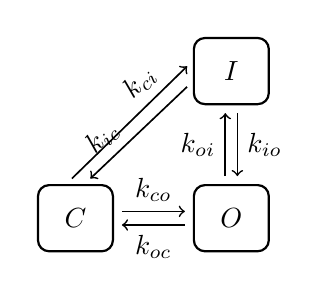
\begin{tikzpicture}[
   font=\sffamily,
   every matrix/.style={ampersand replacement=\&,column sep=1cm,row sep=1cm},
   state/.style={draw,thick,rounded corners,inner sep=.3cm},
   to/.style={->,semithick,shorten >=0.1cm,shorten <=0.1cm},
   Q/.style={->,semithick,sloped,pos=0.700000,shorten >=0.1cm,shorten <=0.1cm}, 
   every node/.style={auto}]
\matrix{
\&\node[state] (I) {\parbox{10pt}{\centerline{$I$}}};\\
\node[state] (C) {\parbox{10pt}{\centerline{$C$}}};\&\node[state] (O) {\parbox{10pt}{\centerline{$O$}}};\\
};
\draw[to]  (O.100) to node {$k_{oi}$} (I.260);
\draw[to]  (O.190) to node {$k_{oc}$} (C.350);
\draw[to]  (I.280) to node {$k_{io}$} (O.80);
\draw[Q]  (I.195) to node {$k_{ic}$} (C.75);
\draw[to]  (C.10) to node {$k_{co}$} (O.170);
\draw[Q]  (C.105) to node {$k_{ci}$} (I.165);
\end{tikzpicture}
\end{center}
\caption{Three-state Markov model. In the mutant case, we
replace the rates $k_{ci}$ and $k_{oi}$ by  $k_{ci}/\mu$ and $k_{oi}/\mu$, 
respectively, where $\mu$ denotes the mutation severity index.}
\label{MOT_mut_L/ICO.pdf}%
\end{figure}


%\fig[0.5]{MOT_mut_L/ICO.pdf}{Three state Markov model. In the mutant case we
%replace the rates $k_{ci}$ and $k_{oi}$ by  $k_{ci}/\mu$ and $k_{oi}/\mu$ where
%$\mu$ denotes the mutation severity index.}



\subsection{A theoretical open state blocker}



We observed above that to repair the effect of changes in the mean
open time, it is necessary to use an open state blocker. The reason for this is 
that neither a closed blocker nor an inactivated blocker has any effect on the 
mean open time and, therefore, it is inconceivable that such blockers 
can repair the effect of a mutation on the mean open time. An open state blocker 
directly affects the mean open time and the drug must be tuned to repair the 
effect of the mutation.

A Markov model that includes an open state blocker is shown in 
Figure \ref{MOT_mut_L/BICO_O.pdf}.
We have already computed
formulas for the equilibrium probabilities of a Markov model of this form (see
page \pageref{Ionchannels_L/BICO.pdf}). The inverse $(p=1/o)$ open probability in equilibrium is given by
\[
p_{\mu}=1+\frac{k_{oc}}{k_{co}}+\frac{1}{\mu}\frac{k_{oi}}{k_{io}}%
\]
and thus the wild type inverse open probability is given by%
\[
p=1+\frac{k_{oc}}{k_{co}}+\frac{k_{oi}}{k_{io}}.
\]
Similarly, the inverse open probability in the presence of the open state blocker 
is given by%
\[
p_{b,\mu}=1+\frac{k_{oc}}{k_{co}}+\frac{1}{\mu}\frac{k_{oi}}{k_{io}}+\frac{k_{ob}%
}{k_{bo}}.
\]
Furthermore, the mean open time of wild type is given by%
\[
\tau_{o}=\frac{1}{k_{oi}+k_{oc}}%
\]
and, when the theoretical drug is included in the mutant case, the mean open
time is given by%
\[
\tau_{o,b,\mu}=\frac{1}{\frac{1}{\mu}k_{oi}+k_{oc}+k_{ob}}.
\]
We are now looking for a drug that will repair the equilibrium probability and
the mean open time. More precisely, we want to find the parameters $k_{bo}$
and $k_{ob}$ such that $p_{b,\mu}=p$ and $\tau_{o,b,\mu}=\tau_{o}$. More explicitly, we require that
\[
1+\frac{k_{oc}}{k_{co}}+\frac{1}{\mu}\frac{k_{oi}}{k_{io}}+\frac{k_{ob}%
}{k_{bo}}=1+\frac{k_{oc}}{k_{co}}+\frac{k_{oi}}{k_{io}}\text{ }%
\]
and%
\[
\frac{1}{\mu}k_{oi}+k_{oc}+k_{ob}=k_{oi}+k_{oc}.
\]
This is a $2\times 2$ system of equations in the unknowns $k_{ob}$ and $k_{bo}$ and the 
solution is given by
\begin{equation}
k_{ob}=\left(  1-\mu^{-1}\right)  k_{oi}\text{ and }k_{bo}=k_{io}.\label{mot_in_dr}%
\end{equation}
We will see in numerical experiments below that the open state blocker
illustrated in Figure  \ref{MOT_mut_L/BICO_O.pdf} where the parameters of the drug are given by (\ref{mot_in_dr})
repairs the effect of the mutation.

\begin{figure}[ptb]
\begin{center}
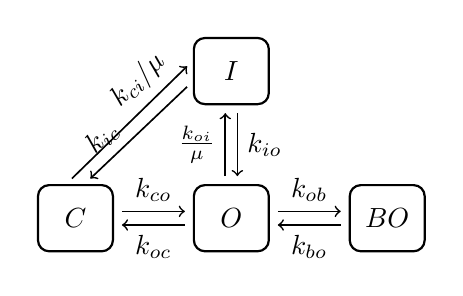
\begin{tikzpicture}[
   font=\sffamily,
   every matrix/.style={ampersand replacement=\&,column sep=1cm,row sep=1cm},
   state/.style={draw,thick,rounded corners,inner sep=.3cm},
   to/.style={->,semithick,shorten >=0.1cm,shorten <=0.1cm},
   Q/.style={->,semithick,sloped,pos=0.700000,shorten >=0.1cm,shorten <=0.1cm},  
   every node/.style={auto}]
\matrix{
\&\node[state] (I) {\parbox{10pt}{\centerline{$I$}}};\&\\
\node[state] (C) {\parbox{10pt}{\centerline{$C$}}};\&\node[state] (O) {\parbox{10pt}{\centerline{$O$}}};\&\node[state] (BO) {\parbox{10pt}{\centerline{$BO$}}};\\
};
\draw[to]  (O.100) to node {$\frac{k_{oi}}{\mu}$} (I.260);
\draw[to]  (O.190) to node {$k_{oc}$} (C.350);
\draw[to]  (O.10) to node {$k_{ob}$} (BO.170);
\draw[to]  (I.280) to node {$k_{io}$} (O.80);
\draw[Q]  (I.195) to node {$k_{ic}$} (C.75);
\draw[to]  (C.10) to node {$k_{co}$} (O.170);
\draw[Q]  (C.105) to node {$k_{ci}/\mu$} (I.165);
\draw[to]  (BO.190) to node {$k_{bo}$} (O.350);
\end{tikzpicture}
\end{center}
\caption{The model represented in Figure  \ref{MOT_mut_L/ICO.pdf} is extended 
to account for the blocker (BO) associated with the open state.}
\label{MOT_mut_L/BICO_O.pdf}
\end{figure}

%\fig[0.7]{MOT_mut_L/BICO_O.pdf}{The model represented in Figure  \ref{MOT_mut_L/ICO.pdf} extended to account for
%the blocker (BO) associated the open state.}


\subsection{Probability density functions using the open state blocker}

We have found a theoretical drug (see $\left(  \ref{mot_in_dr}\right)$) for
the mutation affecting the rates from O to I and from C to I and we want to
assess the drug's usefulness by considering the open probability density
functions. For the wild type case, the probability density functions of the
states present in the Markov model of Figure \ref{MOT_mut_L/ICO.pdf} are
governed by the system%


\begin{align}
\frac{\partial}{\partial v}\left(  a_{o}\rho_{o}\right)   &  =k_{co}\rho
_{c}-\left(  k_{oc}+k_{oi}\right)  \rho_{o}+k_{io}\rho_{i},\nonumber\\
\frac{\partial}{\partial v}\left(  a_{c}\rho_{c}\right)   &  =k_{oc}\rho
_{o}-\left(  k_{co}+k_{ci}\right)  \rho_{c}+k_{ic}\rho_{i},\label{wt_mt_in}\\
\frac{\partial}{\partial v}\left(  a_{c}\rho_{i}\right)   &  =k_{oi}\rho
_{o}-(k_{io}+k_{ic})\rho_{i}+k_{ci}\rho_{c}.\nonumber
\end{align}
In the mutant case, when the open state blocker is added as indicated in Figure
\ref{MOT_mut_L/BICO_O.pdf}, the probability density system is%
\begin{align}
\frac{\partial}{\partial v}\left(  a_{o}\rho_{o}\right)   &  =k_{co}\rho
_{c}-\left(  k_{oc}+\frac{1}{\mu}k_{oi}+k_{ob}\right)  \rho_{o}+k_{io}\rho_{i}%
+k_{bo}\rho_{b},\nonumber\\
\frac{\partial}{\partial v}\left(  a_{c}\rho_{c}\right)   &  =k_{oc}\rho
_{o}-\left(  k_{co}+\frac{1}{\mu}k_{ci}\right)  \rho_{c}+k_{ic}\rho
_{i},\label{mot_dr_123}\\
\frac{\partial}{\partial v}\left(  a_{c}\rho_{i}\right)   &  =\frac{1}{\mu
}k_{oi}\rho_{o}-(k_{io}+k_{ic})\rho_{i}+\frac{1}{\mu}k_{ci}\rho_{c}%
,\nonumber\\
\frac{\partial}{\partial v}\left(  a_{c}\rho_{b}\right)   &  =k_{ob}\rho
_{o}-k_{bo}\rho_{b}.\nonumber
\end{align}
%\K{zzz Skal man ikke i den f\o rste ligningen  i (\ref{mot_dr_123}) ha med leddet $-k_{ob}\rho_{o}$? I s\r{a} fall m\r{a} man vel ogs\r{a} endre fra  $\left(  k_{oc}+\frac{1}{\mu}k_{oi}\right)  \rho_{o}$ til $\left(  k_{oc}+k_{oi}\right)  \rho_{o}$ i den f\o rste ligningen i (\ref{mot_dr_124})?}
%{\bf xxx Glenn: I have corrected the text according to Karoline; can you check the code?}
%\G{This was correct in the code. In general, models are implemented based on the  figure, not the math. (And diagonal entries are computed automatically.)}
As usual, $\rho_{o},\rho_{c},\rho_{i},$ and $\rho_{b}$ denote the probability density
functions of the open, closed, inactivated, and blocked states, respectively,
and the functions of the flux are given by $\left(  \ref{vflux_mot}\right)  .$ By introducing
the drug given by $\left(  \ref{mot_in_dr}\right)  $, we obtain the system
\begin{align}
\frac{\partial}{\partial v}\left(  a_{o}\rho_{o}\right)   &  =k_{co}\rho
_{c}-\left(  k_{oc}+k_{oi}\right)  \rho_{o}+k_{io}\rho_{i}%
+k_{io}\rho_{b},\nonumber\\
\frac{\partial}{\partial v}\left(  a_{c}\rho_{c}\right)   &  =k_{oc}\rho
_{o}-\left(  k_{co}+\frac{1}{\mu}k_{ci}\right)  \rho_{c}+k_{ic}\rho
_{i},\label{mot_dr_124}\\
\frac{\partial}{\partial v}\left(  a_{c}\rho_{i}\right)   &  =\frac{1}{\mu
}k_{oi}\rho_{o}-(k_{io}+k_{ic})\rho_{i}+\frac{1}{\mu}k_{ci}\rho_{c}%
,\nonumber\\
\frac{\partial}{\partial v}\left(  a_{c}\rho_{b}\right)   &  =\left(
1-\mu^{-1}\right)  k_{oi}\rho_{o}-k_{io}\rho_{b}.\nonumber
\end{align}
In Figure \ref{MOT/iocb.pdf}, we show solutions of the wild type system 
$\left(\ref{wt_mt_in}\right)  $, the mutant system, and the mutant system where the
drug is added $\left(  \ref{mot_dr_124}\right)  $. Note that the mutant system
is equal to the wild type system, except for the change of the rates $k_{ci}$
and $k_{oi}$ given by
\begin{align}
\bar{k}_{ci} &  =k_{ci}/\mu,\\
\bar{k}_{oi} &  =k_{oi}/\mu.\nonumber
\end{align}
In Figure \ref{MOT/iocb.pdf},  we compare the open probability density functions of the three models for three
different sets of parameters. In the left panel of Figure \ref{MOT/iocb.pdf},  we show the open probability of the wild type (solid line),
 the mutant ($\mu=10$), and the mutant in the presence of the theoretical open blocker. We see that the effect of the
 mutation is completely repaired by the drug. Other cases are shown in the center and right panels. The effect of the drug is still good but the effect of the mutation is not completely repaired. These observations are confirmed in Table \ref{tab:iocb}.
Furthermore, we have  tested a large variety of parameters and the results 
we show here (center and right panels)  represent the most difficult cases we could find in experiments. 
Therefore, we conclude that the theoretical open state blocker illustrated in Figure  \ref{MOT_mut_L/BICO_O.pdf}
 works very well. 

\fig{MOT/iocb.pdf}{Left panel: All rates equal one. The theoretical drug restores $\rho_o$. Middle panel: As in the left panel, except $k_{co}=10\text{ ms}^{-1}$. 
Right panel:  As in the left panel, except $k_{io}=0.1\text{ ms}^{-1}$. For all three cases, $\mu = 10$.}
%\G{Jeg har testet hver parameter for seg, fra 0.01 til 100. Det er kun disse parameterne som kan gi betydelige avvik, og det blir ikke verre en det vises her, som jo egentlig er ganske bra.}} 

%{\bf xxx Glenn: Can you compute the usual statistical properties of the three cases of 
%Figure \ref{MOT_mut_L/BICO_O.pdf} and put it in a table?}
%\G{This is now Table \ref{tab:iocb}}

\begin{table}  \begin{center}
\begin{tabular}{|c|r|r|r|r|r|r|} \hline
& \multicolumn{2}{c|}{$k=1$} &
\multicolumn{2}{c|}{$k_{co}=10$} &
\multicolumn{2}{c|}{$k_{io}=0.1$}  \\ \cline{2-7}
 & $\pi_o$ & $E_o$ & $\pi_o$ & $E_o$ & $\pi_o$ & $E_o$ \\ \hline
WT&0.333 & 16.366 & 0.476 & 22.995 & 0.083 & -12.867 \\ \hline
MT&0.476 & 23.272 & 0.833 & 31.074 & 0.333 & 17.702 \\ \hline
MT+OB&0.333 & 16.366 & 0.476 & 23.169 & 0.083 & -9.225 \\ \hline
\end{tabular} \end{center}
\caption{Statistical properties of $\rho_o$ for the cases shown in Figure \ref{MOT/iocb.pdf}.\label{tab:iocb}}
\end{table}


\subsection{Stochastic simulations using the open state blocker}

In Figure \ref{MOT/iocb_mc.pdf}, we show simulations using the numerical scheme%
\begin{equation}
v_{n+1}=v_{n}-\Delta t\left(  g_{K}\left(  v_{n}-V_{K}\right)  +\gamma
_{n}g_{Na}(v_{n}-V_{Na}\right)  ), \label{s1000}%
\end{equation}
where the value of the variable $\gamma_{n}$ 
is determined by the Markov model given in
Figure \ref{MOT_mut_L/ICO.pdf}. For the wild type case, the rates $k_{ci}$ and $k_{oi}$
are used and, in the mutant case, the rates $k_{ci}/\mu$ and $k_{oi}%
/\mu$ are used. Furthermore, when the drug is applied in the mutant case, the Markov
model is as illustrated in Figure \ref{MOT_mut_L/BICO_O.pdf}, where the rates of
the drug are given by $\left(\ref{mot_in_dr}\right).$ We observe that, in the
mutant case, the channel does not inactivate and therefore more action
potentials are generated. When the drug is applied, this effect seems to be removed and
the channel again acts more or less as in the wild type case. However, as mentioned above
it is not straightforward to compare solutions based on the stochastic model and therefore we emphasis
the use of probability density functions. 

\fig[0.6]{MOT/iocb_mc.pdf}{Monte Carlo runs of the case shown in the right panel of Figure \ref{MOT/iocb.pdf}.}

\section{Notes}

\begin{enumerate}
\item The derivation of the formula for the mean open time given by (\ref{tau_o}) can be found in many
places (e.g., Keener and Sneyd \cite{KeenerSneyd} or Smith \cite{Smith2002}). 
\end{enumerate}




\chapter[The burst mode]{The burst mode of the mutant sodium channel \label{burst_chap}}

We observed above that the effect of the $\Delta$KPQ mutation of the SCN5A
gene leading to a delayed sodium current can be modeled by increasing the
reaction rates from the inactivated state to the open state and to the
permissible state $C_{0}$. The model gave results at least qualitatively 
similar to the experimental data (see Figure \ref{NaM/mc.pdf}). 

A better-established way of
modeling the effect of the mutation is to introduce a so-called burst mode.
A simple Markov model including a burst mode is illustrated in Figure \ref{burst_prototype}, where the states of the burst mode
are indicated by $\ast$. Note that when the channel is in the burst mode,
there is no inactivated state and therefore the burst mode can be used to model the effect of impaired inactivation.
The reaction rates going from the burst mode to
the normal mode are given by $k^{u}$ (where $u$ stands for up) and the reaction rates from the normal mode
to the burst mode are given by $k^{d}$
(where $d$ stands for down). We assume $k^{d}<<k^{u}$, which means that, for the wild type, 
the probability of being in the burst mode is very small. The probability
of being in the burst mode increases with the mutation severity index $\mu$.
As usual, $\mu=1$ represents the wild type. In the wild type, a channel is basically never in the burst mode and therefore the channel inactivates as it should and no late sodium current is observed. In the mutant case, however, the probability of being in the burst mode is increased. Since there is no inactivated state in the burst mode, the channel fails to inactivate and therefore the probability of being in the open state is increased and therefore we observe a non-negligible late current. This will be illustrated in the numerical computations below.

\begin{figure}[ptb]
\begin{center}
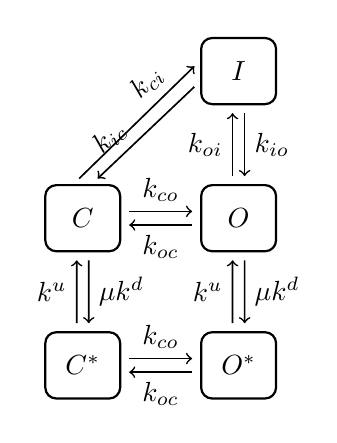
\begin{tikzpicture}[
   font=\sffamily,
   every matrix/.style={ampersand replacement=\&,column sep=1cm,row sep=1cm},
   state/.style={draw,thick,rounded corners,inner sep=.3cm},
   to/.style={->,semithick,shorten >=0.1cm,shorten <=0.1cm},
   Q/.style={->,semithick,sloped,pos=0.700000,shorten >=0.1cm,shorten <=0.1cm},  
   every node/.style={auto}]
\matrix{
\&\node[state] (I) {\parbox{10pt}{\centerline{$I$}}};\\
\node[state] (C) {\parbox{10pt}{\centerline{$C$}}};\&\node[state] (O) {\parbox{10pt}{\centerline{$O$}}};\\
\node[state] (C^{*}) {\parbox{10pt}{\centerline{$C^{*}$}}};\&\node[state] (O^{*}) {\parbox{10pt}{\centerline{$O^{*}$}}};\\
};
\draw[to]  (O^{*}.100) to node {$k^{u}$} (O.260);
\draw[to]  (O^{*}.190) to node {$k_{oc}$} (C^{*}.350);
\draw[to]  (O.280) to node {$\mu k^{d}$} (O^{*}.80);
\draw[to]  (O.100) to node {$k_{oi}$} (I.260);
\draw[to]  (O.190) to node {$k_{oc}$} (C.350);
\draw[to]  (I.280) to node {$k_{io}$} (O.80);
\draw[Q]  (I.195) to node {$k_{ic}$} (C.75);
\draw[to]  (C.10) to node {$k_{co}$} (O.170);
\draw[Q]  (C.105) to node {$k_{ci}$} (I.165);
\draw[to]  (C.280) to node {$\mu k^{d}$} (C^{*}.80);
\draw[to]  (C^{*}.10) to node {$k_{co}$} (O^{*}.170);
\draw[to]  (C^{*}.100) to node {$k^{u}$} (C.260);
\end{tikzpicture}
\end{center}
\caption{Prototypical model of a sodium channel including a burst mode. 
 The model consists of the states $O,I,$ and $C$ of the normal mode and $O^{*}$ and
$C^{*}$ of the burst mode (lower part). }%
\label{burst_prototype}%
\end{figure}



\section{Equilibrium probabilities}

We will start by considering the equilibrium states of the prototypical
model illustrated in Figure \ref{burst_prototype}. By following the usual steps
(see, e.g., page \pageref{9001}) we find
\begin{comment}
The equilibrium solutions are characterized by
the system of equations%
\begin{align}
k_{io}i  &  =k_{oi}o,\text{ }k_{ci}c=k_{ic}i,\text{ }k_{co}c=k_{oc}o,\\
\mu k^{d}c  &  =k^{u}c^{\ast},\text{ }\mu k^{d}o=k^{u}o^{\ast}.
\end{align}
As usual, all variables can be expressed in terms of the open probability,%
\begin{equation}
i=\frac{k_{oi}}{k_{io}}o,\text{ }c=\frac{k_{oc}}{k_{co}}o,\text{ }c^{\ast
}=\frac{\mu k^{d}}{k^{u}}\frac{k_{oc}}{k_{co}}o,\text{ }o^{\ast}=\frac{\mu
k^{d}}{k^{u}}o,
\end{equation}
and, since $o+i+c+c^{\ast}+o^{\ast}=1,$ we have%
\begin{equation}
\left(  1+\frac{k_{oi}}{k_{io}}+\frac{k_{oc}}{k_{co}}+\frac{\mu k^{d}}{k^{u}%
}\frac{k_{oc}}{k_{co}}+\frac{\mu k^{d}}{k^{u}}\right)  o=1
\end{equation}
and therefore
\end{comment}
 the equilibrium probabilities given by%
\begin{align}
o  &  =\frac{1}{1+\frac{k_{oi}}{k_{io}}+\frac{k_{oc}}{k_{co}}+\frac{\mu k^{d}%
}{k^{u}}\frac{k_{oc}}{k_{co}}+\frac{\mu k^{d}}{k^{u}}},\\
i  &  =\frac{\frac{k_{oi}}{k_{io}}}{1+\frac{k_{oi}}{k_{io}}+\frac{k_{oc}%
}{k_{co}}+\frac{\mu k^{d}}{k^{u}}\frac{k_{oc}}{k_{co}}+\frac{\mu k^{d}}{k^{u}%
}},\\
c  &  =\frac{\frac{k_{oc}}{k_{co}}}{1+\frac{k_{oi}}{k_{io}}+\frac{k_{oc}%
}{k_{co}}+\frac{\mu k^{d}}{k^{u}}\frac{k_{oc}}{k_{co}}+\frac{\mu k^{d}}{k^{u}%
}},\\
c^{\ast}  &  =\frac{\frac{k_{oc}}{k_{co}}\frac{\mu k^{d}}{k^{u}}}%
{1+\frac{k_{oi}}{k_{io}}+\frac{k_{oc}}{k_{co}}+\frac{\mu k^{d}}{k^{u}}%
\frac{k_{oc}}{k_{co}}+\frac{\mu k^{d}}{k^{u}}},\\
o^{\ast}  &  =\frac{\frac{\mu k^{d}}{k^{u}}}{1+\frac{k_{oi}}{k_{io}}%
+\frac{k_{oc}}{k_{co}}+\frac{\mu k^{d}}{k^{u}}\frac{k_{oc}}{k_{co}}+\frac{\mu
k^{d}}{k^{u}}}.
\end{align}
Here, we observe that the equilibrium probability of being in the inactivated
state is clearly reduced as the mutation severity index is increased. This is
the effect we wanted, since inactivation is impaired in the
mutation and the effect is modeled by introducing a burst mode that lacks the
inactivated state. Second, we observe that the sum of the open probabilities
given by%
\begin{equation}
o+o^{\ast}=\frac{1+\mu\frac{k^{d}}{k^{u}}}{1+\frac{k_{oi}}{k_{io}}%
+\frac{k_{oc}}{k_{co}}+\mu\frac{k^{d}}{k^{u}}\frac{k_{oc}}{k_{co}}+\mu
\frac{k^{d}}{k^{u}}}%
\end{equation}
is an increasing function of $\mu;$ in fact,%
\begin{equation}
\frac{d}{d\mu}\left(  o+o^{\ast}\right)  =\frac{\frac{k^{d}}{k^{u}}%
\frac{k_{oi}}{k_{io}}}{\left(  1+\frac{k_{oc}}{k_{co}}+\frac{k_{oi}}{k_{io}%
}+\mu\frac{k^{d}}{k^{u}}\frac{k_{oc}}{k_{co}}+\mu\frac{k^{d}}{k^{u}}\right)
^{2}}>0.
\end{equation}
So the model has the two main properties we seek: The equilibrium
probability of being in the inactivated state is reduced and the open probability
is increased.

\bigskip

\section{The mean open time}

We observed above (see page \pageref{mot_many}) that the formula for the mean open time can also
be derived in the presence of several open states. If we generalize the
argument to also take into account the inactivated state, we find that the
mean open time of the Markov model illustrated in Figure \ref{burst_prototype} is given by%
\begin{equation}
\tau_{o,\mu}=\frac{\mu k^{d}+k^{u}}{\mu k^{d}k_{oc}+k^{u}\left(  k_{oc}%
+k_{oi}\right)  }%
\end{equation}
and, since%
\begin{equation}
\frac{d\tau_{o,\mu}}{d\mu}=\frac{k_{oi}k^{d}k^{u}}{\left(  k^{u}k_{oc}+k^{u}k_{oi}+\mu k_{oc}k^{d}\right)  ^{2}},
\end{equation}
the mean open time increases as a function of the mutation severity index.

%\K{zzz Skal man skifte slik fra $k_{oc}$ og $k_{oi}$ til $k_{co}$ og $k_{io}$
%n\r{a}r man deriverer?}

\bigskip

\section{An optimal theoretical open state blocker}

\begin{figure}[ptb]
\begin{center}
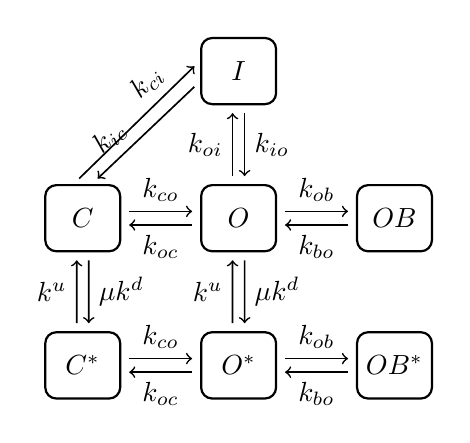
\begin{tikzpicture}[
   font=\sffamily,
   every matrix/.style={ampersand replacement=\&,column sep=1cm,row sep=1cm},
   state/.style={draw,thick,rounded corners,inner sep=.3cm},
   to/.style={->,semithick,shorten >=0.1cm,shorten <=0.1cm},
   Q/.style={->,semithick,sloped,pos=0.700000,shorten >=0.1cm,shorten <=0.1cm},  
   every node/.style={auto}]
\matrix{
\&\node[state] (I) {\parbox{10pt}{\centerline{$I$}}};\&\\
\node[state] (C) {\parbox{10pt}{\centerline{$C$}}};\&\node[state] (O) {\parbox{10pt}{\centerline{$O$}}};\&\node[state] (OB) {\parbox{10pt}{\centerline{$OB$}}};\\
\node[state] (C^{*}) {\parbox{10pt}{\centerline{$C^{*}$}}};\&\node[state] (O^{*}) {\parbox{10pt}{\centerline{$O^{*}$}}};\&\node[state] (OB^{*}) {\parbox{10pt}{\centerline{$OB^{*}$}}};\\
};
\draw[to]  (O^{*}.100) to node {$k^{u}$} (O.260);
\draw[to]  (O^{*}.10) to node {$k_{ob}$} (OB^{*}.170);
\draw[to]  (O^{*}.190) to node {$k_{oc}$} (C^{*}.350);
\draw[to]  (O.280) to node {$\mu k^{d}$} (O^{*}.80);
\draw[to]  (O.100) to node {$k_{oi}$} (I.260);
\draw[to]  (O.190) to node {$k_{oc}$} (C.350);
\draw[to]  (O.10) to node {$k_{ob}$} (OB.170);
\draw[to]  (I.280) to node {$k_{io}$} (O.80);
\draw[Q]  (I.195) to node {$k_{ic}$} (C.75);
\draw[to]  (C.10) to node {$k_{co}$} (O.170);
\draw[Q]  (C.105) to node {$k_{ci}$} (I.165);
\draw[to]  (C.280) to node {$\mu k^{d}$} (C^{*}.80);
\draw[to]  (OB.190) to node {$k_{bo}$} (O.350);
\draw[to]  (OB^{*}.190) to node {$k_{bo}$} (O^{*}.350);
\draw[to]  (C^{*}.10) to node {$k_{co}$} (O^{*}.170);
\draw[to]  (C^{*}.100) to node {$k^{u}$} (C.260);
\end{tikzpicture}
\end{center}
\caption{Prototypical model of a sodium channel including a burst mode and an open state blocker. 
 The model consists of the states $O,I,C,$ and $OB$ of the normal mode and $O^{*},C^{*},$ and $OB^*$ of the burst mode (lower part). 
 The states $OB$ and $OB^*$ represent the open blocker and we assume that the rates characterizing the blocker are the same in the normal and burst modes.}%
\label{burst_prototype_drg}%
\end{figure}


Our aim is now to define an open state drug that can repair both the
equilibrium open probability and the mean open time. The structure of the open
state blocker is given in Figure \ref{burst_prototype_drg} and the equilibrium total open probability is now
given by 
\begin{comment}
the following system of equations:%
\begin{align*}
k_{io}i  &  =k_{oi}o,\text{ }k_{ci}c=k_{ic}i,\text{ }k_{co}c=k_{oc}o,\text{
}k_{bo}b=k_{ob}o,\\
\mu k^{d}c  &  =k^{u}c^{\ast},\text{ }\mu k^{d}o=k^{u}o^{\ast},\text{ }%
k_{bo}b^{\ast}=k_{ob}o^{\ast}.
\end{align*}
Since%
\begin{equation*}
i=\frac{k_{oi}}{k_{io}}o,\text{ }c=\frac{k_{oc}}{k_{co}}o,\text{ }c^{\ast
}=\frac{\mu k^{d}}{k^{u}}\frac{k_{oc}}{k_{co}}o,\text{ }o^{\ast}=\frac{\mu
k^{d}}{k^{u}}o,\text{ }b=\frac{k_{ob}}{k_{bo}}o,\text{ }b^{\ast}=\frac{k_{ob}%
}{k_{bo}}\frac{\mu k^{d}}{k^{u}}o
\end{equation*}
and $o+i+c+c^{\ast}+o^{\ast}+b+b^{\ast}=1,$ 
we obtain the total open probability%
\end{comment}
\begin{equation}
\left(  o+o^{\ast}\right)  _{\mu,d}=\frac{1+\mu\frac{k^{d}}{k^{u}}}{1+\frac
{k_{oi}}{k_{io}}+\frac{k_{oc}}{k_{co}}+\mu\frac{k^{d}}{k^{u}}\frac{k_{oc}%
}{k_{co}}+\mu\frac{k^{d}}{k^{u}}+\frac{k_{ob}}{k_{bo}}\left(  1+\frac{\mu
k^{d}}{k^{u}}\right)  }. \label{o300}%
\end{equation}
Furthermore, the mean open time is now given by%
\begin{equation}
\tau_{o,\mu,d}=\frac{\mu k^{d}+k^{u}}{\mu k^{d}\left(  k_{oc}+k_{ob}\right)
+k^{u}\left(  k_{oc}+k_{oi}+k_{ob}\right)  }, \label{mot300}%
\end{equation}
where the subscript $d$ is used to remind us that this concerns the case where
the theoretical drug has been applied.

\bigskip

The task at hand is now to tune the drug such that the equilibrium open
probability and the mean open time given by $\left(  \ref{o300}\right)  $ and
$\left(  \ref{mot300}\right)  $, respectively, are as close as possible to the equilibrium open
probability and the mean open time of the wild type. We regard the parameters
$k_{ob}$ and $k_{bo}$ as the unknowns and we want to solve the following
$2\times2$ system of equations:%
\begin{align}
\frac{1+\mu\frac{k^{d}}{k^{u}}}{1+\frac{k_{oi}}{k_{io}}+\frac{k_{oc}}{k_{co}%
}+\mu\frac{k^{d}}{k^{u}}\frac{k_{oc}}{k_{co}}+\mu\frac{k^{d}}{k^{u}}%
+\frac{k_{ob}}{k_{bo}}\left(  1+\mu\frac{k^{d}}{k^{u}}\right)  }  &  =\frac
{1+\frac{k^{d}}{k^{u}}}{1+\frac{k_{oi}}{k_{io}}+\frac{k_{oc}}{k_{co}}+\frac{k^{d}}{k^{u}}%
\frac{k_{oc}}{k_{co}}+\frac{k^{d}}{k^{u}}},\label{dr300}\\
\frac{\mu k^{d}+k^{u}}{\mu k^{d}\left(  k_{oc}+k_{ob}\right)  +k^{u}\left(
k_{oc}+k_{oi}+k_{ob}\right)  }  &  =\frac{k^{d}+k^{u}}{k^{d}k_{oc}%
+k^{u}\left(  k_{oc}+k_{oi}\right)  }, \label{dr301}%
\end{align}
where the latter equation determines the on rate, $k_{ob},$ of the drug,%
\begin{equation}
k_{ob}=\left(  \mu-1\right)  \frac{k^{d}k^{u}k_{oi}}{\left(  k^{u}+\mu
k^{d}\right)  \left(  k^{u}+k^{d}\right)  }, \label{kob300}%
\end{equation}
and we note that, in the case of $\mu=1,$ the  drug is completely turned off,
which is reasonable. Since $k_{ob}$ is known, the off rate of the drug can be
computed by solving $\left(  \ref{dr300}\right).$ If we define%
\begin{equation}
A=\frac{k_{ob}}{k_{bo}},
\end{equation}
we find from $\left(  \ref{dr300}\right)$  
\begin{equation}
A=(\mu-1)\frac{k_{oi}}{k_{io}}  \frac{k^{u}k^{d}}{\left(  \mu k^{d}+k^{u}\right)  \left(  k^{d}%
+k^{u}\right)  \label{Akbo}}
\end{equation}
and then the off rate of the drug is given by%
\begin{equation}
k_{bo}=A^{-1}k_{ob}=k_{io} \label{kbo300}
\end{equation}
which is the same as we have in the prototypical model given in 
Figure \ref{MOT_mut_L/BICO_O.pdf}; see (\ref{mot_in_dr}) on page \pageref{mot_in_dr}.


\bigskip

\section{Numerical experiments}

\graytable{l}{
{|c|c|} \hline
$\mu$ & 20 \\ \hline
$k_u$ & 0.0001 $\rm{ms^{-1}}$\\ \hline
$k_d$ & 0.001 $\rm{ms^{-1}}$\\ \hline
$k_{ob}$ & 0.0286 $\rm{ms^{-1}}$\\ \hline
$k_{bo}$ &0.000824 $\rm{ms^{-1}}$\\ \hline
}{Values of the parameters used in the model in Figure \ref{burst_prototype_drg}.
The remaining rates  are as in Table \ref{markov_rates}.
\label{tab:burst_ob}}

The purpose of this section is to show how the burst mode can be used to represent impaired inactivation and how the theoretical drug derived above works. 

\subsection{Representation of the late sodium current using the burst mode model}

As discussed in Chapter \ref{simple_Na}, impaired inactivation leads to a late sodium current (see Figure \ref{NaM/mc.pdf}). Here, we will see that this effect can also be obtained using a Markov model of the form indicated in Figure \ref{burst_prototype}. In Figure \ref{NaB/current.pdf}, we repeat the computations reported in Figure \ref{NaM/mc.pdf}, using the Markov model of Figure \ref{burst_prototype}. The parameters used in this computation are given in Table \ref{tab:burst_ob}. We observe from Figure \ref{NaB/current.pdf} that $\mu=20$ seems to represent the late current of Figure \ref{NaM/mc.pdf} fairly well. 
 
 \subsection{The open state blocker repairs the effect of the mutation}

In Figure \ref{NaB/current.pdf}, we show the late current for the wild type, the mutant $\mu=20$, and the drug using the optimal open state blocker defined by (\ref{kob300}) and (\ref{kbo300}). We observe that the late current induced by the mutation is  repaired by the open state blocker. The statistics of the open probability density function (for the wild type, the mutant ($\mu=20$), and the mutant where the drug has been applied) are given in Table \ref{tab:burst_stat} and  
the corresponding probability density functions are shown in Figure \ref{NaB/ob.pdf}. Again we note that the open blocker repairs the main features of the solution.



\fig{NaB/current.pdf}{Currents computed using the Markov model illustrated in Figure \ref{burst_prototype_drg}. 
The simulations are based on averages of 10,000 runs. As expected, the open blocker asymptotically repairs the late current. }

%\fig{NaB/current_zoom.pdf}{Just to illustrate that things work as expected, we might not want to use this one.}

\fig{NaB/ob.pdf}{Stationary probability density functions computed using the Markov model illustrated in Figure
\ref{burst_prototype_drg}. The open probability density function is given in the left panel and the probability density function of the sum of non-conducting states is given in the right panel. We observe that the open blocker repairs most parts of the probability density functions.}

\begin{table}  \begin{center}
\begin{tabular}{|r|r|r|r|r|} \hline
$\mu$ & $\pi_o$ & $\pi_n$ & $E_o$ & $E_n$ \\ \hline
1 & 0.59 & 0.41 & 31.2 & -54.2 \\ \hline
20 & 0.96 & 0.04 & 33.1 & -52.8 \\ \hline
50 & 0.98 & 0.02 & 33.1 & -51.3 \\ \hline
100 & 0.99 & 0.01 & 33.2 & -49.8 \\ \hline
20+OB & 0.46 & 0.54 & 30.2 & -57.9 \\ \hline
\end{tabular} \end{center}
\caption{Statistics of the stationary probability density functions computed using the Markov model illustrated in Figure
\ref{burst_prototype_drg}. The subscript $o$ refers to open states and the subscript $n$ refers to non-conducting states.
 \label{tab:burst_stat}}
\end{table}



\section{A more sophisticated Markov model \label{sophisticated}}

The Markov model presented in Figure \ref{burst_prototype} above has a structure that is a bit simpler than
the Markov model commonly used to model the sodium channel. A more common structure is given in 
Figure \ref{wtreac330}. This is the model we studied in Chapter \ref{simple_Na}. When a burst mode is added to it, the Markov model obtains the form illustrated in Figure \ref{burst}.


\begin{figure}[ptb]
\begin{center}
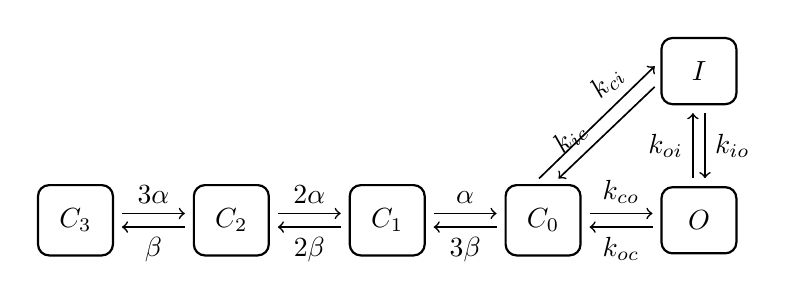
\begin{tikzpicture}[
   font=\sffamily,
   every matrix/.style={ampersand replacement=\&,column sep=1cm,row sep=1cm},
   state/.style={draw,thick,rounded corners,inner sep=.3cm},
   to/.style={->,semithick,shorten >=0.1cm,shorten <=0.1cm},
   Q/.style={->,semithick,sloped,pos=0.700000,shorten >=0.1cm,shorten <=0.1cm},  
   every node/.style={auto}]
\matrix{
\&\&\&\&\node[state] (I) {\parbox{10pt}{\centerline{$I$}}};\\
\node[state] (C_{3}) {\parbox{10pt}{\centerline{$C_{3}$}}};\&\node[state] (C_{2}) {\parbox{10pt}{\centerline{$C_{2}$}}};\&\node[state] (C_{1}) {\parbox{10pt}{\centerline{$C_{1}$}}};\&\node[state] (C_{0}) {\parbox{10pt}{\centerline{$C_{0}$}}};\&\node[state] (O) {\parbox{10pt}{\centerline{$O$}}};\\
};
\draw[to]  (O.100) to node {$k_{oi}$} (I.260);
\draw[to]  (O.190) to node {$k_{oc}$} (C_{0}.350);
\draw[to]  (I.280) to node {$k_{io}$} (O.80);
\draw[Q]  (I.195) to node {$k_{ic}$} (C_{0}.75);
\draw[to]  (C_{0}.10) to node {$k_{co}$} (O.170);
\draw[Q]  (C_{0}.105) to node {$k_{ci}$} (I.165);
\draw[to]  (C_{0}.190) to node {$3\beta$} (C_{1}.350);
\draw[to]  (C_{1}.10) to node {$\alpha$} (C_{0}.170);
\draw[to]  (C_{1}.190) to node {$2\beta$} (C_{2}.350);
\draw[to]  (C_{2}.10) to node {$2\alpha$} (C_{1}.170);
\draw[to]  (C_{2}.190) to node {$\beta$} (C_{3}.350);
\draw[to]  (C_{3}.10) to node {$3\alpha$} (C_{2}.170);
\end{tikzpicture}
\end{center}
\caption{Typical Markov model of a wild type sodium channel consisting of an open
state $(O)$, an inactivated state $(I)$, and four closed states $(C_{0}%
,C_{1},C_{2}, \text{ and }C_{3})$. This model was analyzed in Chapter \ref{simple_Na}.}%
\label{wtreac330}%
\end{figure}



\begin{figure}[ptb]
\begin{center}
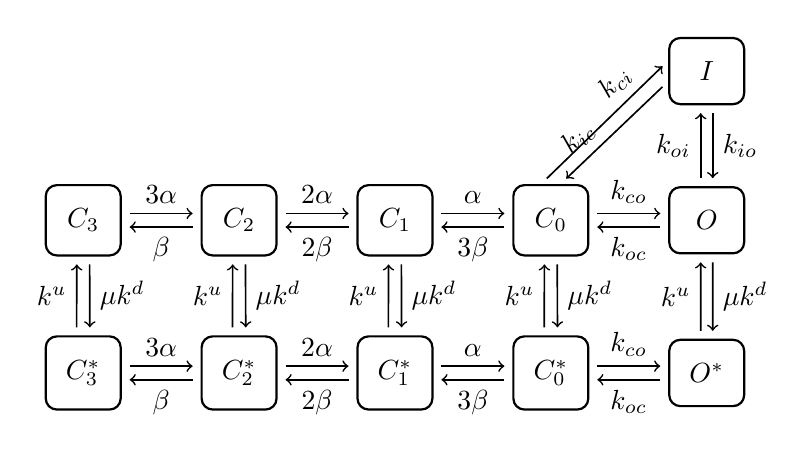
\begin{tikzpicture}[
   font=\sffamily,
   every matrix/.style={ampersand replacement=\&,column sep=1cm,row sep=1cm},
   state/.style={draw,thick,rounded corners,inner sep=.3cm},
   to/.style={->,semithick,shorten >=0.1cm,shorten <=0.1cm},
   Q/.style={->,semithick,sloped,pos=0.700000,shorten >=0.1cm,shorten <=0.1cm},  
   every node/.style={auto}]
\matrix{
\&\&\&\&\node[state] (I) {\parbox{10pt}{\centerline{$I$}}};\\
\node[state] (C_{3}) {\parbox{10pt}{\centerline{$C_{3}$}}};\&\node[state] (C_{2}) {\parbox{10pt}{\centerline{$C_{2}$}}};\&\node[state] (C_{1}) {\parbox{10pt}{\centerline{$C_{1}$}}};\&\node[state] (C_{0}) {\parbox{10pt}{\centerline{$C_{0}$}}};\&\node[state] (O) {\parbox{10pt}{\centerline{$O$}}};\\
\node[state] (C_{3}^{*}) {\parbox{10pt}{\centerline{$C_{3}^{*}$}}};\&\node[state] (C_{2}^{*}) {\parbox{10pt}{\centerline{$C_{2}^{*}$}}};\&\node[state] (C_{1}^{*}) {\parbox{10pt}{\centerline{$C_{1}^{*}$}}};\&\node[state] (C_{0}^{*}) {\parbox{10pt}{\centerline{$C_{0}^{*}$}}};\&\node[state] (O^{*}) {\parbox{10pt}{\centerline{$O^{*}$}}};\\
};
\draw[to]  (O^{*}.100) to node {$k^{u}$} (O.260);
\draw[to]  (O^{*}.190) to node {$k_{oc}$} (C_{0}^{*}.350);
\draw[to]  (O.280) to node {$\mu k^{d}$} (O^{*}.80);
\draw[to]  (O.100) to node {$k_{oi}$} (I.260);
\draw[to]  (O.190) to node {$k_{oc}$} (C_{0}.350);
\draw[to]  (I.280) to node {$k_{io}$} (O.80);
\draw[Q]  (I.195) to node {$k_{ic}$} (C_{0}.75);
\draw[to]  (C_{0}.10) to node {$k_{co}$} (O.170);
\draw[Q]  (C_{0}.105) to node {$k_{ci}$} (I.165);
\draw[to]  (C_{0}.190) to node {$3\beta$} (C_{1}.350);
\draw[to]  (C_{0}.280) to node {$\mu k^{d}$} (C_{0}^{*}.80);
\draw[to]  (C_{1}.10) to node {$\alpha$} (C_{0}.170);
\draw[to]  (C_{1}.190) to node {$2\beta$} (C_{2}.350);
\draw[to]  (C_{1}.280) to node {$\mu k^{d}$} (C_{1}^{*}.80);
\draw[to]  (C_{2}.10) to node {$2\alpha$} (C_{1}.170);
\draw[to]  (C_{2}.190) to node {$\beta$} (C_{3}.350);
\draw[to]  (C_{2}.280) to node {$\mu k^{d}$} (C_{2}^{*}.80);
\draw[to]  (C_{3}.10) to node {$3\alpha$} (C_{2}.170);
\draw[to]  (C_{3}.280) to node {$\mu k^{d}$} (C_{3}^{*}.80);
\draw[to]  (C_{0}^{*}.10) to node {$k_{co}$} (O^{*}.170);
\draw[to]  (C_{0}^{*}.100) to node {$k^{u}$} (C_{0}.260);
\draw[to]  (C_{0}^{*}.190) to node {$3\beta$} (C_{1}^{*}.350);
\draw[to]  (C_{1}^{*}.100) to node {$k^{u}$} (C_{1}.260);
\draw[to]  (C_{1}^{*}.10) to node {$\alpha$} (C_{0}^{*}.170);
\draw[to]  (C_{1}^{*}.190) to node {$2\beta$} (C_{2}^{*}.350);
\draw[to]  (C_{2}^{*}.100) to node {$k^{u}$} (C_{2}.260);
\draw[to]  (C_{2}^{*}.10) to node {$2\alpha$} (C_{1}^{*}.170);
\draw[to]  (C_{2}^{*}.190) to node {$\beta$} (C_{3}^{*}.350);
\draw[to]  (C_{3}^{*}.100) to node {$k^{u}$} (C_{3}.260);
\draw[to]  (C_{3}^{*}.10) to node {$3\alpha$} (C_{2}^{*}.170);
\end{tikzpicture}
\end{center}\caption{Markov model of the sodium channel. The model consists of the states
$O,I,C_{0},C_{1},C_{2},$ and $C_{3}$ of the normal mode and $O^{*},C^{*}%
_{0},C^{*}_{1},C^{*}_{2},$ and $C^{*}_{3}$ of the burst mode (lower part). Note
that there is no inactivated state in the burst mode and that $\mu$ denotes
the mutation severity index. A larger value of $\mu$ increases the probability
of moving from the normal (upper) mode to the burst (lower) mode.}%
\label{burst}%
\end{figure}

To understand how the burst mode changes the properties of the model,
it is of interest to compute the equilibrium probabilities. 
%\begin{comment}
The equilibrium state of the model presented in Figure \ref{burst} is
characterized by the following system of equations:%
\begin{equation}%
\begin{array}
[c]{ccc}%
k_{ci}c_{0}=k_{ic}i, & k_{oi}o=k_{io}i, & k_{co}c_{0}=k_{oc}o,\\
3\beta c_{0}=\alpha c_{1}, & 2\alpha c_{2}=2\beta c_{1}, & 3\alpha c_{3}=\beta c_{2},\\
k^{u}o^{\ast}=\mu k^{d}o, & k^{u}c_{0}^{\ast}=\mu k^{d}c_{0}, & k^{u}%
c_{1}^{\ast}=\mu k^{d}c_{1},\\
k^{u}c_{2}^{\ast}=\mu k^{d}c_{2}, & k^{u}c_{3}^{\ast}=\mu k^{d}c_{3}. &
\end{array}
\label{ep1}
\end{equation}
It follows that%
\begin{align*}
i &  =\frac{k_{oi}}{k_{io}}o,\text{ }c_{0}=\frac{k_{oc}}{k_{co}}o,\text{ }\\
c_{1} &  =\frac{3\beta}{\alpha}\frac{k_{oc}}{k_{co}}o,\text{ }c_{2}%
=\frac{3\beta^{2}}{\alpha^{2}}\frac{k_{oc}}{k_{co}}o,\text{ }c_{3}=\frac
{\beta^{3}}{\alpha^{3}}\frac{k_{oc}}{k_{co}}o,\\
o^{\ast} &  =\mu\frac{k^{d}}{k^{u}}o,c_{0}^{\ast}=\mu\frac{k^{d}}{k^{u}}%
\frac{k_{oc}}{k_{co}}o,c_{1}^{\ast}=\mu\frac{3\beta}{\alpha}\frac{k^{d}}%
{k^{u}}\frac{k_{oc}}{k_{co}}o,\\
c_{2}^{\ast} &  =\mu\frac{3\beta^{2}}{\alpha^{2}}\frac{k^{d}}{k^{u}}%
\frac{k_{oc}}{k_{co}}o,c_{3}^{\ast}=\mu\frac{\beta^{3}}{\alpha^{3}}\frac
{k^{d}}{k^{u}}\frac{k_{oc}}{k_{co}}o
\end{align*}
and, since the sum of the probabilities equals one, we have%
%\end{comment}
\[
o\left(  \mu\right)  =\frac{1}{\frac{k_{oi}}{k_{io}}+\left(  1+\mu\frac{k^{d}%
}{k^{u}}\right)  \left(  1+\frac{k_{oc}}{k_{co}}\left(  1+\beta/\alpha\right)
^{3}\right)  }
\]
and
\[
o\left(  \mu\right)  +o^{\ast}\left(  \mu\right)  =\frac{1+\mu\frac{k^{d}%
}{k^{u}}}{\frac{k_{oi}}{k_{io}}+\left(  1+\mu\frac{k^{d}}{k^{u}}\right)
\left(  1+\frac{k_{oc}}{k_{co}}\left(  1+\beta/\alpha\right)  ^{3}\right)  }.%
\]
Therefore,
\[
\frac{d}{d\mu}\left(  o\left(  \mu\right)  +o^{\ast}\left(  \mu\right)
\right)  =\frac{\frac{k_{oi}}{k_{io}}\frac{k^{d}}{k^{u}}}{\left(  \frac
{k_{oi}}{k_{io}}+\left(  1+\frac{k_{oc}}{k_{co}}\left(  1+\beta/\alpha\right)
^{3}\right)  \left(  1+\mu\frac{k^{d}}{k^{u}}\right)  \right)  ^{2}}>0,%
\]
so the total open probability increases as the mutation severity index
$\mu$ increases. This will lead to a sustained sodium current characteristic
of the mutation under consideration. 

It is also interesting to see how the mutation severity index changes the
probability of being in the normal or burst mode. To understand
this, we define $b$ and $b^{\ast}$ as the sum of the probabilities in the
normal and burst modes, respectively. By using the equilibrium probabilities
derived above, we obtain
\[
\frac{b^{\ast}}{b}=\frac{o^{\ast}+c_{0}^{\ast}+c_{1}^{\ast}+c_{2}^{\ast}%
+c_{3}^{\ast}}{o+c_{0}+c_{1}+c_{2}+c_{3}+i}=\mu\frac{k^{d}}{k^{u}}%
\frac{1+\frac{k_{oc}}{k_{co}}\left(  1+\beta/\alpha\right)  ^{3}}%
{\frac{k_{oi}}{k_{io}}+1+\frac{k_{oc}}{k_{co}}\left(  1+\beta/\alpha\right)
^{3}}%
\]
and thus the probability of being in the burst mode increases as the mutation
severity index increases.

\bigskip

\section[Numerical experiments; burst mode]{Numerical experiments illustrating the effect of the burst mode}

\graytable{l}{
{|c|c|} \hline
$\mu$ & 1,10,30,100 \\ \hline
$k_u$ & 0.1 $\rm{ms^{-1}}$\\ \hline
$k_d$ & 0.01 $\rm{ms^{-1}}$\\ \hline
%$k_{ob}$ &  0.2196 $\rm{ms^{-1}}$\\ \hline
%$k_{bo}$ &0.0001578 $\rm{ms^{-1}}$\\ \hline
}{Values of the parameters used in the model in Figure \ref{burst}.
%\ref{burstdrg}.
The remaining rates  are as in Table \ref{markov_rates} on page \pageref{markov_rates}. \label{tab:burst_param}
}


The effect of increasing the mutation severity index of the Markov model given in Figure \ref{burst} is shown in
 Figure \ref{NaB/pdf3.pdf} using the parameters given in Table \ref{tab:burst_param}.
  %In the computations we use the parameters $k_u=0.1, k_d = 0.01$ and the mutation severity index is $\mu=1,10,30,100$ where $\mu=1$ (solid line) represents the wild type. 
 The associated currents are shown in Figure
 \ref{NaB/mc.pdf} and we note that when the mutation severity index increases, there is a significant late sodium current.
 
\fig{NaB/pdf3.pdf}{ The probability density functions of the open, closed, and inactivated states for the
burst mode model. The mutation severity index is given by $\mu=10,$ $30,$ and $100$ and the black line represents the wild type.
Note that we only show solutions for the values of the transmembrane potential where the solutions differ as a result of the mutations.}

%\fig{NaB/mc.pdf}{\G{Top trace is WT, the other ones MT, with the lowest corresponding to $\mu=100$.} 
%Current from the burst model. Stronger mutations leads to slower closing of the channel.}


\begin{figure}[p]\centering
\vbox{
\includegraphics[width=0.9\linewidth]{NaB/mc.pdf}
\includegraphics[width=0.7\linewidth]{NaM/Bennet.png}
}
\caption{Currents computed using the Markov model including the burst mode (see Figure \ref{burst}). Top panel: Current for $\mu=1,$ $10,$ $30,$ $100$. Each trace is an average of 10,000 Monte Carlo runs and the current is computed by  $I=g_{Na} P_o (v-V_{Na})$, with the transmembrane potential at $v=0$ mV. The currents are normalized so that the wild type current peaks at -1. Here $V_{Na} = 45$ mV and $g_{Na} = 1$ mS/$\mbox{cm}^2$.  The lower figures are from Bennett et al. \cite{Bennett1995}.\label{NaB/mc.pdf}}
\end{figure}


%\begin{table}  \begin{center}
%\begin{tabular}{|r|r|r|r|r|r|r|} \hline
%$\mu$ & $\pi_o$ & $\pi_c$ & $\pi_i$ & $\rho_o$ & $\rho_c$ & $\rho_i$ \\ \hline
%1 & 0.00006 & 0.99961 & 0.00033 & -53.2 & -84.9 & -73.4 \\ \hline
%10 & 0.00008 & 0.99967 & 0.00024 & -26.1 & -84.9 & -67.5 \\ \hline
%30 & 0.00012 & 0.99969 & 0.00019 & -8.3 & -84.9 & -61.0 \\ \hline
%100 & 0.00022 & 0.99963 & 0.00015 & 10.5 & -84.9 & -54.2 \\ \hline
%\end{tabular} \end{center}
%\caption{ Expected values of the transmembrane potential for open, closed or inactivated
%states for increasing values of the mutation severity index $\mu$.} \label{tab:burst}
%\end{table}
\begin{table}  \begin{center}
\begin{tabular}{|r|r|r|r|r|} \hline
$\mu$ & $1000 \times \pi_o$ & $\pi_n$ & $E_o$ & $E_c$ \\ \hline
1 & 0.05738 &  0.99994 & -53.2 & -84.9 \\ \hline
10 & 0.08435 & 0.99992 & -26.1 & -84.9 \\ \hline
30 & 0.12109 & 0.99983 & -8.3 & -84.9 \\ \hline
100 & 0.22305 & 0.99978 & 10.5 & -84.9 \\ \hline
30+OB & 0.05490&0.99995 & -57.0 & -84.9 \\ \hline
\end{tabular} \end{center}
\caption{Probabilities and expected values of the transmembrane potential for open and non-conducting states for increasing values of the mutation severity index $\mu$.} \label{tab:burst}
\end{table}


%xxx Glenn xxx: repeat experiments of the previous model. That is repeat figure 11.3, table 11.2, figure 11.4.



\section[Theoretical drug for the burst mode model]{A theoretical drug for the
mutation represented by the burst mode}

 In the simplified Markov model presented in Figure \ref{burst_prototype} above, we saw
that an open blocker was able to repair the effect of the mutation.
Now the Markov model is extended (see Figure \ref{burst}), but it is reasonable to
believe that an open blocker is still the best alternative, since both the open
probability and the mean open time are affected by the mutation. We consider
the Markov model given in Figure \ref{burstdrg}, where an open blocker is added to both
the open states of the Markov model given in Figure \ref{burst}. 
\begin{comment}
The equilibrium state
of the Markov model given in Figure \ref{burstdrg} is characterized by%
\begin{equation}%
\begin{array}
[c]{ccc}%
k_{ci}c_{0}=k_{ic}i, & k_{oi}o=k_{io}i, & k_{co}c_{0}=k_{oc}o,\\
3\beta c_{0}=\alpha c_{1}, & 2\alpha c_{2}=2\beta c_{1}, & 3\alpha c_{3}=\beta
c_{2},\\
k^{u}o^{\ast}=\mu k^{d}o, & k^{u}c_{0}^{\ast}=\mu k^{d}c_{0}, & k^{u}%
c_{1}^{\ast}=\mu k^{d}c_{1},\\
k^{u}c_{2}^{\ast}=\mu k^{d}c_{2}, & k^{u}c_{3}^{\ast}=\mu k^{d}c_{3}, & \\
k_{ob}o=k_{bo}b, & k_{ob}o^{\ast}=k_{bo}b^{\ast}. &
\end{array}
\end{equation}
\end{comment}
By following our usual procedure, we find that%
\begin{comment}
\begin{align*}
i &  =\frac{k_{oi}}{k_{io}}o,\text{ }c_{0}=\frac{k_{oc}}{k_{co}}o,\text{ }\\
c_{1} &  =\frac{3\beta}{\alpha}\frac{k_{oc}}{k_{co}}o,\text{ }c_{2}%
=\frac{3\beta^{2}}{\alpha^{2}}\frac{k_{oc}}{k_{co}}o,\text{ }c_{3}=\frac
{\beta^{3}}{\alpha^{3}}\frac{k_{oc}}{k_{co}}o,\\
o^{\ast} &  =\mu\frac{k^{d}}{k^{u}}o,c_{0}^{\ast}=\mu\frac{k^{d}}{k^{u}}%
\frac{k_{oc}}{k_{co}}o,c_{1}^{\ast}=\mu\frac{3\beta}{\alpha}\frac{k^{d}}%
{k^{u}}\frac{k_{oc}}{k_{co}}o,\\
c_{2}^{\ast} &  =\mu\frac{3\beta^{2}}{\alpha^{2}}\frac{k^{d}}{k^{u}}%
\frac{k_{oc}}{k_{co}}o,c_{3}^{\ast}=\mu\frac{\beta^{3}}{\alpha^{3}}\frac
{k^{d}}{k^{u}}\frac{k_{oc}}{k_{co}}o,\\
b &  =\frac{k_{ob}}{k_{bo}}o,b^{\ast}=\mu\frac{k_{ob}}{k_{bo}}\frac{k^{d}%
}{k^{u}}o,
\end{align*}
\newline and, since the sum of the probabilities equals one, we have
\end{comment}
\[
\left(  o+o^{\ast}\right)  _{\mu,d}=\frac{1+\mu\frac{k^{d}}{k^{u}}}%
{\frac{k_{ob}}{k_{bo}}\left(  1+\mu\frac{k^{d}}{k^{u}}\right)  +\frac{k_{oi}%
}{k_{io}}+\left(  1+\mu\frac{k^{d}}{k^{u}}\right)  \left(  1+\frac{k_{oc}%
}{k_{co}}\left(  1+\beta/\alpha\right)  ^{3}\right)  }.
\]
The associated mean open time is given by%
\begin{equation}
\tau_{o,\mu,d}=\frac{\mu k^{d}+k^{u}}{\mu k^{d}\left(  k_{oc}+k_{ob}\right)
+k^{u}\left(  k_{oc}+k_{oi}+k_{ob}\right)  }.
\end{equation}
We now want to tune the drug characterized by the two parameters $k_{ob}$
and $k_{bo}$ such that
\[
\left(  o+o^{\ast}\right)  _{\mu,d}\approx\left(  o+o^{\ast}\right)  _{wt}%
\]
and%
\[
\tau_{o,\mu,d}\approx\tau_{o,wt},%
\]
where the subscript {\it wt} denotes wild type values. As above, we have two equations
for the two unknowns  $k_{ob}$ and $k_{bo}$ and the solution is given by%
\begin{equation}
k_{ob}=\left(  \mu-1\right)  \frac{k^{d}k^{u}k_{oi}}{\left(  k^{u}+\mu
k^{d}\right)  \left(  k^{u}+k^{d}\right)  } \label{na_drug_ob}
\end{equation}
and%
\begin{equation}
k_{bo}=A^{-1}k_{ob},
\end{equation}
where%
\begin{equation}
A=\frac{k_{oi}}{k_{io}}k^{u}k^{d}\frac{\mu-1}{\left(  \mu k^{d}+k^{u}\right)
\left(  k^{d}+k^{u}\right)  }.
\end{equation}
So we obtain
\begin{equation}
k_{bo}=k_{io}. \label{na_drug_bo}
\end{equation}
We note that the formulas for the optimal open blocker for the Markov model
given in Figure \ref{burstdrg} are exactly the same as for the open blocker of the prototype Markov
model given in Figure \ref{burst_prototype_drg}.


\begin{figure}[ptb]
\begin{center}
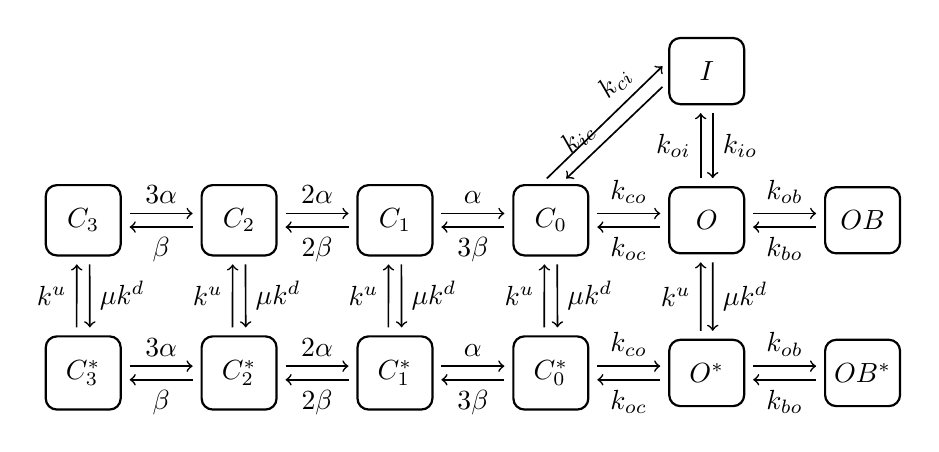
\begin{tikzpicture}[
   font=\sffamily,
   every matrix/.style={ampersand replacement=\&,column sep=1cm,row sep=1cm},
   state/.style={draw,thick,rounded corners,inner sep=.3cm},
   to/.style={->,semithick,shorten >=0.1cm,shorten <=0.1cm},
   Q/.style={->,semithick,sloped,pos=0.700000,shorten >=0.1cm,shorten <=0.1cm},  
   every node/.style={auto}]
\matrix{
\&\&\&\&\node[state] (I) {\parbox{10pt}{\centerline{$I$}}};\&\\
\node[state] (C_{3}) {\parbox{10pt}{\centerline{$C_{3}$}}};\&\node[state] (C_{2}) {\parbox{10pt}{\centerline{$C_{2}$}}};\&\node[state] (C_{1}) {\parbox{10pt}{\centerline{$C_{1}$}}};\&\node[state] (C_{0}) {\parbox{10pt}{\centerline{$C_{0}$}}};\&\node[state] (O) {\parbox{10pt}{\centerline{$O$}}};\&\node[state] (OB) {\parbox{10pt}{\centerline{$OB$}}};\\
\node[state] (C_{3}^{*}) {\parbox{10pt}{\centerline{$C_{3}^{*}$}}};\&\node[state] (C_{2}^{*}) {\parbox{10pt}{\centerline{$C_{2}^{*}$}}};\&\node[state] (C_{1}^{*}) {\parbox{10pt}{\centerline{$C_{1}^{*}$}}};\&\node[state] (C_{0}^{*}) {\parbox{10pt}{\centerline{$C_{0}^{*}$}}};\&\node[state] (O^{*}) {\parbox{10pt}{\centerline{$O^{*}$}}};\&\node[state] (OB^{*}) {\parbox{10pt}{\centerline{$OB^{*}$}}};\\
};
\draw[to]  (O^{*}.100) to node {$k^{u}$} (O.260);
\draw[to]  (O^{*}.10) to node {$k_{ob}$} (OB^{*}.170);
\draw[to]  (O^{*}.190) to node {$k_{oc}$} (C_{0}^{*}.350);
\draw[to]  (O.280) to node {$\mu k^{d}$} (O^{*}.80);
\draw[to]  (O.100) to node {$k_{oi}$} (I.260);
\draw[to]  (O.190) to node {$k_{oc}$} (C_{0}.350);
\draw[to]  (O.10) to node {$k_{ob}$} (OB.170);
\draw[to]  (I.280) to node {$k_{io}$} (O.80);
\draw[Q]  (I.195) to node {$k_{ic}$} (C_{0}.75);
\draw[to]  (C_{0}.10) to node {$k_{co}$} (O.170);
\draw[Q]  (C_{0}.105) to node {$k_{ci}$} (I.165);
\draw[to]  (C_{0}.190) to node {$3\beta$} (C_{1}.350);
\draw[to]  (C_{0}.280) to node {$\mu k^{d}$} (C_{0}^{*}.80);
\draw[to]  (C_{1}.10) to node {$\alpha$} (C_{0}.170);
\draw[to]  (C_{1}.190) to node {$2\beta$} (C_{2}.350);
\draw[to]  (C_{1}.280) to node {$\mu k^{d}$} (C_{1}^{*}.80);
\draw[to]  (C_{2}.10) to node {$2\alpha$} (C_{1}.170);
\draw[to]  (C_{2}.190) to node {$\beta$} (C_{3}.350);
\draw[to]  (C_{2}.280) to node {$\mu k^{d}$} (C_{2}^{*}.80);
\draw[to]  (C_{3}.10) to node {$3\alpha$} (C_{2}.170);
\draw[to]  (C_{3}.280) to node {$\mu k^{d}$} (C_{3}^{*}.80);
\draw[to]  (OB.190) to node {$k_{bo}$} (O.350);
\draw[to]  (OB^{*}.190) to node {$k_{bo}$} (O^{*}.350);
\draw[to]  (C_{0}^{*}.10) to node {$k_{co}$} (O^{*}.170);
\draw[to]  (C_{0}^{*}.100) to node {$k^{u}$} (C_{0}.260);
\draw[to]  (C_{0}^{*}.190) to node {$3\beta$} (C_{1}^{*}.350);
\draw[to]  (C_{1}^{*}.100) to node {$k^{u}$} (C_{1}.260);
\draw[to]  (C_{1}^{*}.10) to node {$\alpha$} (C_{0}^{*}.170);
\draw[to]  (C_{1}^{*}.190) to node {$2\beta$} (C_{2}^{*}.350);
\draw[to]  (C_{2}^{*}.100) to node {$k^{u}$} (C_{2}.260);
\draw[to]  (C_{2}^{*}.10) to node {$2\alpha$} (C_{1}^{*}.170);
\draw[to]  (C_{2}^{*}.190) to node {$\beta$} (C_{3}^{*}.350);
\draw[to]  (C_{3}^{*}.100) to node {$k^{u}$} (C_{3}.260);
\draw[to]  (C_{3}^{*}.10) to node {$3\alpha$} (C_{2}^{*}.170);
\end{tikzpicture}
\end{center}
\caption{Markov model of the mutant sodium channel with a blocker associated
with the open states. The model consists of the states $O,I,OB,C_{0}%
,C_{1},C_{2},$ and $C_{3}$ of the normal mode and $OB^*,O^{*},C^{*}_{0},C^{*}%
_{1},C^{*}_{2},$ and $C^{*}_{3}$ of the burst mode (lower part). The drug is
characterized by the two parameters $k_{bo}$ and $k_{ob}$.}%
\label{burstdrg}
\end{figure}

\newpage

%\subsection{Numerical experiments}
%\graytable{l}{
%{|c|c|} \hline
%$\mu$ & 30\\ \hline
%$k_{ob}$ &  0.2196 $\rm{ms^{-1}}$\\ \hline
%$k_{bo}$ &0.0001578 $\rm{ms^{-1}}$\\ \hline
%}{Values of the parameters used in the model in Figure \ref{burstdrg}.
%%\ref{burstdrg}. 
%The remaining rates are as in Table \ref{tab:burst_param}.
%}


In Figure \ref{NaB/pdf3_d.pdf}, we show the probability density functions of the wild type, the mutant (using $\mu=30$), and
the mutant case where the optimal open blocker is applied. The blocker repairs the effect of the mutation and the same effect is seen in Figure \ref{NaB/mc_d.pdf} where the currents are given; the open blocker removes the late sodium current.


\fig{NaB/pdf3_d.pdf}{Probability density functions for the wild type, the mutant ($\mu=30$), and the mutant in the presence of the open blocker. The subscripts $o$ and $n$ refer to open and non-conduction states, respectively, where the states are shown in  Figure \ref{burstdrg}.}
\fig{NaB/mc_d.pdf}{Currents computed using the Markov model given in Figure \ref{burstdrg}
for the wild type, the mutant ($\mu=30$), and the mutant in the presence of the open blocker.}

\clearpage

\section{Notes \label{notesburst}}

\begin{enumerate}
\item The burst mode is discussed by Bennett et al. \cite{Bennett1995} and modeled
in the paper by Clancy and Rudy \cite{Clancy1999}.
\item The form of the model illustrated in Figure \ref{burst} is taken from Clancy and
Rudy \cite{Clancy1999}, but the functions and parameters of the model are not
taken from their paper.
\item As mentioned above, the introduction of a burst mode is a convenient way of modeling the effect of certain mutations. The notion that gating may enter various modes has been considerably extended and studied in the papers by Chakrapani et al. \cite{ Chakrapani2007a, Chakrapani2007b, Chakrapani2011} and by Ionescu et al. \cite{Ionescu2007}. In the recent paper by Siekmann et al \cite{Siekmann2014} the concept of modal gating is studied and a method for detecting mode changes based on single channel data is developed.
\end{enumerate}

\chapter[Whole cell action potentials]{Action potentials: Summing up the effect of loads of ion channels \label{ap}}
    
    In this final chapter we will use the theoretical drugs developed in various chapters above for whole cell simulations. So far we have studied very small parts of a cell. We started by studying the dynamics going on in a single dyad; see Figure \ref{cicr_1D}. The size of one dyad is 
less than 1/1000 $\mu \mbox{m}^3$\cite{Bers2001} and we have been concerned with the concentration of calcium ions in this small volume. We have also studied the voltage dynamics in the vicinity of a single ion channel. The size of a single channel is about \GTLV{1 nm}. Now we address what is going on in a whole cell and it is important to realize that, compared to the single dyad and the single ion channel, the whole cell is huge; a normal ventricular cell is about 30,000 $\mu \mbox{m}^3$  \cite{Bers2001}, or on the order of  30 million times larger than the single dyad.
   
    In the analysis of single channels, we have regarded the state of a channel as a stochastic variable. In the whole cell, however, the effect of a huge number of channels is added and the sum can be modeled using deterministic equations. We will still use the same Markov model formalism in terms of reaction schemes to formulate the models, but now we will use the associated master equations (see page \pageref{master_equation}) to define the open probability of the channel. Thus we need to solve deterministic systems of ordinary differential equations to find the open probability as a function of time.
    
    Since the state of the channels will be represented using Markov model reaction schemes, we can study mutations in the same manner as we did for the single channel case. Therefore, we can use the results we derived above regarding optimal theoretical drugs for the single channel case for the whole cell case as well. The reasoning behind this was indicated earlier: If a mathematical model of a cell is constructed by using models of a huge number of single channels and we can repair the function of each single channel, the whole cell will be repaired.
    
    In this chapter we will start by introducing a model of the action potential of the whole cell. We will focus on a simplified model that will merely represent the action potential in a qualitatively relevant manner; it will not represent any particular action potential in a quantitatively correct manner.   Using numerical experiments, we will show that the model provides reasonable results for both wild type and various mutations. Finally, we will use the optimal theoretical drugs derived above and see that the effect of various mutations can be repaired using the theoretical drugs.

\section{Whole cell action potential model \label{sec:ap}}
 
    
Our aim is now to introduce a reasonably simple action potential model for a whole cell. We will use the building blocks developed above and add some new features in order to get an action potential that is qualitatively reasonable. 


\begin{figure}
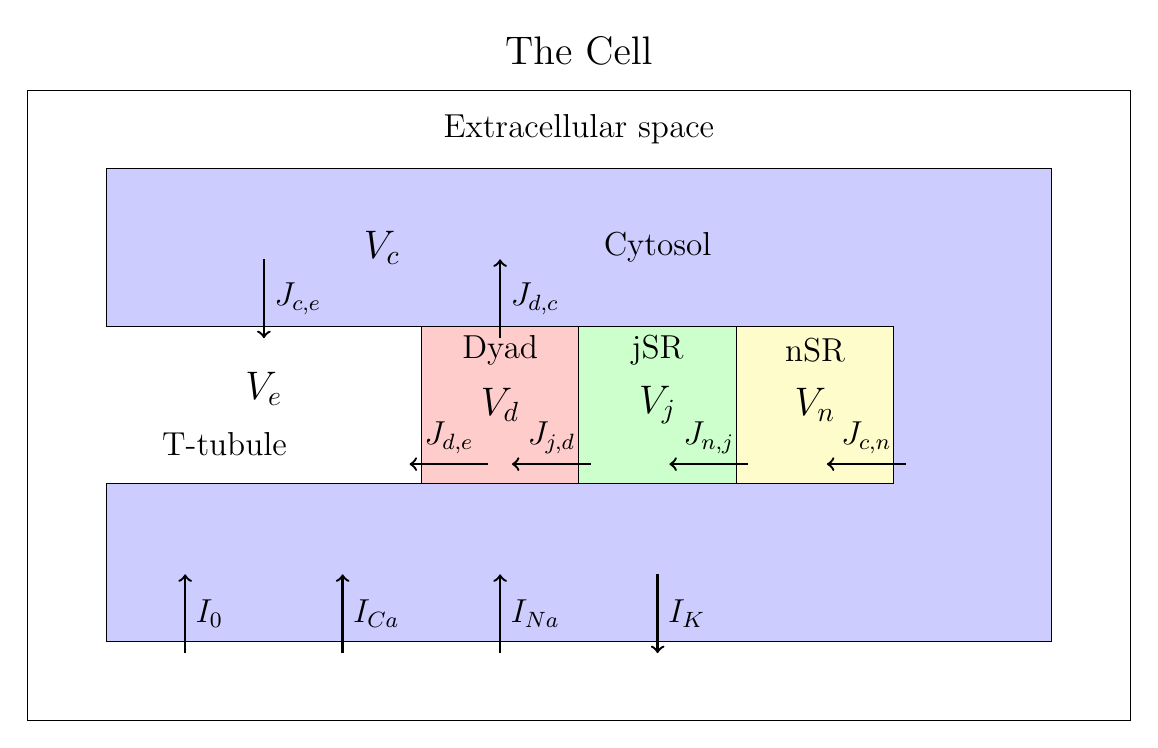
\begin{tikzpicture}[line width=0.3mm]
\tikzstyle{every node}=[font=\large]
\draw[line width=0,fill=white!80!white] (-1,-1) -- (13,-1) -- (13,7) -- (-1,7) -- (-1,-1);
\draw[line width=0,fill=white!80!blue] (0,0) -- (12,0) -- (12,6) -- (0,6)  -- (0,4) -- (10,4) -- (10,2) -- (0,2) -- (0,0);
\draw[line width=0,fill=white!80!yellow] (8,2) -- (10,2) -- (10,4) -- (8,4) -- (8,2);
\draw[line width=0,fill=white!80!green] (6,2) -- (8,2) -- (8,4) -- (6,4) -- (6,2);
\draw[line width=0,fill=white!80!red] (4,2) -- (6,2) -- (6,4) -- (4,4) -- (4,2);
\node[black!50!black] at (5, 3.0) {\Large{$V_{d}$}};
\node[black!50!black] at (7, 3.0) {\Large{$V_{j}$}};
\node[black!50!black] at (9, 3.0) {\Large{$V_{n}$}};
\node[black!50!black] at (5, 3.7) {Dyad};
\node[black!50!black] at (7, 3.7) {jSR};
\node[black!50!black] at (9, 3.7) {nSR};
\draw[->, black] (5,3.85) --node[right] {$J_{d,c}$} (5,4.85);
\draw[->, black] (2,4.85) --node[right] {$J_{c,e}$} (2,3.85);
\node[black!50!black] at (3.5, 5) {\Large{$V_{c}$}};
\node[black!50!black] at (2, 3.2) {\Large{$V_{e}$}};
\node[black!50!black] at (1.5, 2.5) {T-tubule};
\node[black!50!black] at (6, 6.5) {Extracellular space};
\node[black!50!black] at (7, 5) {Cytosol};
\node[black!50!black] at (6, 7.5) {\Large{The Cell}};
\draw[<-, black] (3.85,2.25) --node[above] {$J_{d,e}$} (4.85,2.25);
\draw[->, black] (6.15,2.25) --node[above] {$J_{j,d}$} (5.15,2.25);
\draw[->, black] (8.15,2.25) --node[above] {$J_{n,j}$} (7.15,2.25);
\draw[->, black] (10.15,2.25) --node[above] {$J_{c,n}$} (9.15,2.25);
\draw[->, black] (1,-0.15) --node[right] {$I_{0}$} (1,0.85);
\draw[->, black] (3,-0.15) --node[right] {$I_{Ca}$} (3,0.85);
\draw[->, black] (5,-0.15) --node[right] {$I_{Na}$} (5,0.85);
\draw[<-, black] (7,-0.15) --node[right] {$I_{K}$} (7,0.85);
%\draw[<->, black] (9,-0.15) --node[right] {$I_{NaK}$} (9,0.85);
\end{tikzpicture}
\caption{Sketch of the calcium dynamics and the fluxes and pumps involved. The volumes of the cytosol, the dyad, the junctional sarcoplasmic reticulum (JSR) and the network sarcoplasmic reticulum (NSR) are $V_c,\, V_d,\, V_j,$ and $V_n$, respectively.\label{fig:sketch}}
\end{figure}




The model consists of six main variables: $v, \, c_{e}, \, c_{c}, \, c_{d}, \, c_{j}$, and $c_{n}.$
Here $v,$ as usual, denotes the transmembrane potential given in mV. All the
other variables are concentrations given in $\mu$M; $c_{e}$ is the extracellular calcium concentration, $c_{c}$ is the cytosolic
concentration, $c_{d}$ is the concentration of the dyad, $c_{j}$ is the
concentration of the JSR, and finally $c_{n}$ is the concentration of the NSR;
see Figure \ref{fig:sketch}. In addition to these six main variables, we will have
variables associated with various Markov models; all these variables are between zero
and one; they also denote probabilities and they have no unit. The transmembrane
potential is governed by the equation%
\begin{equation}
Cv^{\prime}=-\left(  I_{Na}+I_{Ca}+I_{K}+I_{0}\right)  \label{dvdt50}%
\end{equation}
where the minus sign is according to convention in the field. Here $C$ denotes the
capacitance and is simply a constant that will be specified below. The current
$I_{0}$ represents a stimulus of the cell and we will use it below to initiate
action potentials. The sodium current $I_{Na},$ the calcium current $I_{Ca},$
and the potassium current $I_{K}$ need some attention and will be handled
separately. 

\bigskip 
In addition to the transmembrane potential, we need to keep track of
all five calcium concentrations. 
%We will assume that the extracellular calcium concentration $c_{e}$ is given and that it is kept constant for all time; it will just enter as a paramter in the computations. But theconcentrations $c_{c},c_{d},c_{j}$ and $c_{n}$ must be updated dynamically. 
By considering Figure \ref{fig:sketch}, we see that the cytosolic concentration can change in
three ways:\footnote{This is a major simplification; many other things can
happen to calcium but this rough description is sufficient for our purposes.
} (1) Calcium may diffuse into the cytosolic space from the
dyad,\footnote{It is important to recall here that when we talk about the dyad
now, we really refer to a space representing the sum of all the dyads of the
cell. So what used to be a very tiny place is not so tiny anymore.} leading to
an increase in the cytosolic concentrations; (2) it can be pumped from the cytosol into the
NSR and thereby reduce the cytosolic concentration; or, finally, (3) it can be
pumped out to the extracellular space, thereby reducing the cytosolic
concentration. The calcium concentration of the NSR, $c_{n},$ will be
increased as calcium is pumped into this space from the cytosol and reduced
by diffusion into its neighboring space, the JSR. In the JSR the calcium
concentration will increase through diffusion from the NSR and be reduced when
calcium is released through the ryanodine receptor (RyR) into the dyadic space. Finally, the
concentration in the dyad will increase when calcium is released from the JSR
to the dyad; it will be reduced as calcium diffuses out to the cytosol and
finally it will be increased when calcium is released into the dyad through
the L-type calcium channels (LCCs). In mathematical terms, we get the following system of
equations:%
\begin{align}
V_{c}c_{c}^{\prime}  & =J_{d,c}-J_{c,n}-J_{c,e},\label{c51}\\
V_{n}c_{n}^{\prime}  & =J_{c,n}-J_{n,j},\label{c52}\\
V_{j}c_{j}^{\prime}  & =J_{n,j}-J_{j,d},\label{c53}\\
V_{d}c_{d}^{\prime}  & =J_{j,d}-J_{d,c}-J_{d,e}.\label{c54} \\
V_{e}c_{e}^{\prime}  & =J_{c,e}+J_{d,e}.\label{c55}%
\end{align}
Here the notation $J_{x,y}$ denotes a flux of calcium from space $x$ to 
space $y.$ So $J_{d,c}$ denotes the flux of calcium from the dyad ($d$) to
the cytosol ($c$) and, similarly, $J_{d,e}$ denotes the flux of calcium from
the  dyad ($d$)  to the extracellular ($e$) space. Here $V_{x}$ denotes the
volume fraction occupied by the space $x.$  The total amount of calcium in the system is given by%
\begin{equation}
c=V_{c}c_{c}+V_{n}c_{n}+V_{j}c_{j}+V_{d}c_{d}+V_{e}c_{e}. \label{tot_ca}
\end{equation}


%\fig{Ap_L/ca_dyn.pdf}{Sketch of the calcium dynamics and the fluxes and pumps involved. The volume of the cytosol, the dyad, the JSR and the NSR is $V_c,\, V_d,\, V_j,$ and $V_n$, respectively. {\bf xxxGTL: can you professionalize the figure?}}


\subsection{Conservation of calcium}

%Suppose the cell membrane is completely closed so we have%
%\begin{equation}
%J_{d,e}=J_{e,d}=0,
%\end{equation}
%then
It follows from the system $\left(  \ref{c51})-(\ref{c55}\right)  $ that%
\begin{equation}
c^{\prime}=0,
\end{equation}
so the total amount of calcium is conserved no matter how the calcium
dynamics of the cell are organized. 

%This observation motivates a modeling
%requirement for the fluxes across the cell membrane. We are modeling a
%process where the cell is supposed to be stimulated by a current, then undergo
%an action potential of length $T$, and then turn back to a normal resting
%state and wait for another stimulus. 
%In general, we have%
%\begin{equation}
%c^{\prime}=J_{e,d}-J_{d,e}%
%\end{equation}
%and in order for the total calcium concentration to return to the same value
%after an action potential, we need to have%
%\begin{equation}
%c(T)=c(0)
%\end{equation}
%\bigskip and this is satisfied if
%\begin{equation}
%\int_{0}^{T}J_{e,d}dt=\int_{0}^{T}J_{d,e}dt.\label{J_req}%
%\end{equation}
%Below, we will make sure that we tune our parameters such that this requirement (at least approximately) is satisfied.


\subsection{Definition of calcium-related fluxes}

\begin{table}
\begin{center}
\begin{tabular}{|c|c|} \hline
$V_d$ & 0.1\% \\ \hline
$V_j$ & 0.3\% \\ \hline
$V_n$ & 1\% \\ \hline
$V_c$ & 98.6\% \\ \hline
\end{tabular} 
\caption{The table shows the relative size of the intracellular spaces. Note that the volume fractions
of the intracellular space add up to $100\%$. In addition, $V_e$ represents $100\%$ of the extracellular space.
We assume that both the extracellular space and the total intracellular space are 30.4 pL
%The extracellular space is 30.4 pL and we assume that it equals the total intracellular space.
}
\end{center}
\end{table}

\begin{table}
\begin{center}
\begin{tabular}{|c|c|} \hline
$k_{c,n}$ & 0.01 \\ \hline
$k_{j,d}$ & 0.01 \\ \hline
$k_{d,c}$ & 0.001 \\ \hline
$k_{d,e}$ & 0.0001 \\ \hline
$k_{n,j}$ & 0.0001  \\ \hline
$k_{c,e}$ & 0.00001 \\ \hline
\end{tabular} 
\caption{\label{tab:k}Constants used to define the fluxes between the different spaces. The constants are in units of 1/ms.
}
\end{center}
\end{table}

\begin{figure}[ptb]
\begin{center}
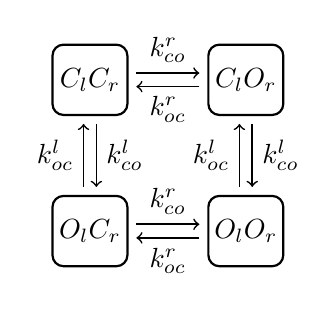
\begin{tikzpicture}[
   font=\sffamily,
   every matrix/.style={ampersand replacement=\&,column sep=1cm,row sep=1cm},
   state/.style={draw,thick,rounded corners,inner sep=.3cm},
   to/.style={->,semithick,shorten >=0.1cm,shorten <=0.1cm},
   Q/.style={->,semithick,sloped,pos=0.700000,shorten >=0.1cm,shorten <=0.1cm},  
   every node/.style={auto}]
\matrix{
\node[state] (C_{l}C_{r}) {\parbox{10pt}{\centerline{$C_{l}C_{r}$}}};\&\node[state] (C_{l}O_{r}) {\parbox{10pt}{\centerline{$C_{l}O_{r}$}}};\\
\node[state] (O_{l}C_{r}) {\parbox{10pt}{\centerline{$O_{l}C_{r}$}}};\&\node[state] (O_{l}O_{r}) {\parbox{10pt}{\centerline{$O_{l}O_{r}$}}};\\
};
\draw[to]  (C_{l}C_{r}.10) to node {$k_{co}^{r}$} (C_{l}O_{r}.170);
\draw[to]  (C_{l}C_{r}.280) to node {$k_{co}^{l}$} (O_{l}C_{r}.80);
\draw[to]  (C_{l}O_{r}.190) to node {$k_{oc}^{r}$} (C_{l}C_{r}.350);
\draw[to]  (C_{l}O_{r}.280) to node {$k_{co}^{l}$} (O_{l}O_{r}.80);
\draw[to]  (O_{l}C_{r}.100) to node {$k_{oc}^{l}$} (C_{l}C_{r}.260);
\draw[to]  (O_{l}C_{r}.10) to node {$k_{co}^{r}$} (O_{l}O_{r}.170);
\draw[to]  (O_{l}O_{r}.100) to node {$k_{oc}^{l}$} (C_{l}O_{r}.260);
\draw[to]  (O_{l}O_{r}.190) to node {$k_{oc}^{r}$} (O_{l}C_{r}.350);
\end{tikzpicture}
\end{center}
\caption{Markov model including four possible states: $C_{l}C_{r}$ (both
closed), $C_{l}O_{r}$ (LCC closed, RyR open), $O_{l}O_{r}$ (both open), and
$O_{l}C_{r}$ (LCC open, RyR closed).}%
\label{eq:m_rl2}%
\end{figure}

%The states of this combined Markov model are given by $C_{l}C_{r}$ (both
%closed), $C_{l}O_{r}$ (LCC closed, RyR open), $O_{l}O_{r}$ (both open), and
%$O_{l}C_{r}$ (LCC open, RyR closed). In our computations, we use the rates shown in Table \ref{fundtions2}.

%following functions%
%\begin{equation}%
\begin{table}
\begin{center}
%\begin{tabular}[c]{|l|l|l|l|} \hline
%$k_{co}^{r}=\mu \frac{x^4}{K(y)^4+x^4}$ & $k_{oc}^{r}=1$ & 
%$K(y) =  K_{max}-y/1000$ & $K_{max} = 7.4\mu$M \\ \hline
%$k_{co}^{l}=\eta\, l_{\infty}(V)/\tau_l$ & $k_{oc}^{l}=(1-l_{\infty}(V))/\tau_l%$ &$l_{\infty}(V) = 0.01 \exp(-(V-5)^2/500)$ 
%&$\tau_l=1$ms \\ \hline
\begin{tabular}[c]{|l|l|} \hline
RyR: & LCC: \\
$k_{co}^{r}(c_d,c_j)=\mu \frac{c_d^4}{K(c_j)^4+c_d^4} \text{ ms}^{-1}$ &$k_{co}^{l}(v)=\eta\, l_{\infty}(v)/\tau_l$ \\
$k_{oc}^{r}=1 \text{ ms}^{-1}$ & $k_{oc}^{l}(v)=(1-l_{\infty}(v))/\tau_l$ \\
$K(c_j) = 20+1000(\frac{1000-c_j}{600})^2$ &  $ l_{\infty}(v) = \exp(-(\frac{v-55}{10})^2)$ \\
 & $\tau_l=1$ ms\\ \hline
\end{tabular}
\end{center}
%\end{equation}
\caption{Reaction rates used in the Markov model illustrated in 
Figure \ref{eq:m_rl2}.
As usual,  $\mu \ge 1$ denotes the mutation severity
index of the RyR and $\eta \ge 1$ denotes the mutation severity
index of the LCC. }
\label{functions2}
\end{table}

We need to define all the fluxes entering the system $\left( \ref{c51})-(\ref{c55}\right)$ and we start with the simple diffusion fluxes. Some of
them have been used in earlier chapters, but we need a little more notation
here, so we redefine all the terms. 

\subsubsection{Flux $J_{d,c}$ from the dyad to the cytosol}
We assume that the pure diffusion flux
from the dyad to the cytosol can be written as%
\begin{equation}
J_{d,c}=k_{d,c}\left(  c_{d}-c_{c}\right).
 \label{J_dc}
\end{equation}
Here we assume that $k_{d,c}$ is a constant and the value used in our computations is given in Table \ref{tab:k}.

\subsubsection{Flux $J_{n,j}$ from the NSR to the JSR}
Similarly, we assume that the diffusion flux from the NSR to the JSR can be written as%
\begin{equation}
J_{n,j}=k_{n,j}\left(  c_{n}-c_{j}\right), \label{J_nj}
\end{equation}
where $k_{n,j}$ is assumed to be a constant (see Table \ref{tab:k}).

\subsubsection{RyR flux $J_{j,d}$ from the JSR to the dyad}
The
flux from the JSR to the dyad can be written in the form%
\begin{equation}
J_{j,d}=o_{j,d}k_{j,d}\left(  c_{j}-c_{d}\right), \label{J_jd}
\end{equation}
where, as usual, $o_{j,d}$ is governed by a Markov model and $k_{j,d}$ is a
constant giving the speed of diffusion when the RyR channel (situated between
the JSR and the dyad) is open. 

The variable $o_{j,d}$ is governed by the Markov model 
used in Chapter \ref{cicr}. For convenience the Markov model is repeated here in Figure \ref{eq:m_rl2} and  the functions
used in the model are given in Table \ref{functions2}. Note that $o_{j,d}$ is the probability of being in the state $C_lO_r$ or the state $O_lO_r$ of the Markov model given in Figure \ref{eq:m_rl2}.

%The parameters and functions are unaltered, except for $K(y)$
%the halv-saturation constant 
%which has been changed to:
%\begin{equation}
%K(y) = 20+1000(\frac{1000-y}{600})^2. \label{halfmax}
%\end{equation}

%have been adapted to the current setting:
%illustrated in Figure xxx and the associated system of ordinary differential equations are given by xxx: 
%\textbf{GTL: Insert the Markov model (ode-system and Figure) that you actually use.}



\subsubsection{Flux from the extracellular space to the dyad: $J_{d,e}$}

 This flux was introduced above (see page \pageref{GHK}) and referred to as the Goldman-Hodgkin-Katz (GHK) flux. In the present notation, we write

\begin{equation}
J_{d,e}=o_{d,e} k_{d,e} \frac{c_d-c_{e}e^{-\frac{v}{v_0}}}{1-e^{-\frac{v}{v_0}}}\frac{v}{v_0}.\label{J_ed}%
\end{equation}
\graytable{l}{
{|c|c|} \hline
$F$ & $96485.3$ C mol$^{-1}$\\ \hline
$R$ & $8.3145$ J mol$^{-1}$K$^{-1}$\\\hline
$T$ & 310 K\\\hline
$v_0$ & 13.357 mV\\ \hline 
}{Parameters in (\ref{J_ed}).\label{FRT_ed}}
Here %$D$ is Fick's diffusion constant, 
$F$ is Faraday's constant, $R$ is the gas constant,
and $T$ is the absolute temperature and we have defined
\[
v_0=\frac{RT}{2F}.%
\]
 The parameters involved in defining the $J_{d,e}$ flux are given in Table \ref{FRT_ed}. Furthermore, $o_{d,e}$ is governed by the Markov model 
 given in Figure \ref{eq:m_rl2}. Here $o_{d,e}$ is the probability of being in the state $O_lC_r$ or the state $O_lO_r$ of the Markov model
  in Figure \ref{eq:m_rl2}.

 
 
%\GTL{used in Chapter 8, see Table \ref{functions2}. The parameters and functions are unaltered, except for $l_{\infty}$  which has been changed to:
%\[ l_{\infty}(v) = \exp(-(\frac{v-55}{10})^2). \]
%}
%presented in Figure xxx. The associated system of ordinary differential equations is given by xxxGTLxxx.
%xxx. \textbf{GTL: Insert the LCC model (ode-system and Figure) that you
%actually use (I do not if you want to couple the two models or treat them
%separately (LCC and RYR).}




\subsection{Definition of calcium pumps}


The terms $J_{c,e}$ and $J_{c,n}$ remain to be defined. These terms are active
fluxes, or pumps, that continuously remove calcium from the cytosol
and out to the extracellular domain $(J_{c,e})$ and into the NSR $(J_{c,n}).$
These pumps transport calcium against a considerable concentration gradient and
the operation therefore requires energy. In our model we do not track the
energy consumption and we simply introduce the pumps:%
\begin{equation}
J_{c,e}=k_{c,e} (c_c-c_e/18000)  \label{J_ce}
\end{equation}
and%
\begin{equation}
J_{c,n}= k_{c,n} (c_c-c_n/10000).  \label{J_cn}
\end{equation}


%xxx \textbf{GTL: insert the pumps you are using (follow the notational convention).}

\subsection{Definition of the currents}

The currents $I_{Na},\, I_K$ and $I_{Ca}$ of (\ref{dvdt50}) remain to be defined. Each current will be written in the form
\[
I_x=o_x g_x (v-v_x),
\]
where  $o_x$ is the open probability of the channel given by the continuous version of a Markov model, $g_x$ is the maximum conductance of the channel, and $v_x$ is the resting potential.

\subsubsection{Sodium current $I_{Na}$}

The sodium current has been studied above; see Chapters \ref{simple_Na} and \ref{burst_chap}. The model takes the form
\begin{equation}
I_{Na}= o_{Na} g_{Na}(v-v_{Na}),   \label{J_Na}
\end{equation}
where the open probability $o_{Na}$ is the sum of the probability of being in the $O$ or the $O^*$ state of the Markov model of Figure  \ref{wtreac3300}. 

\begin{figure}[ptb]
\begin{center}
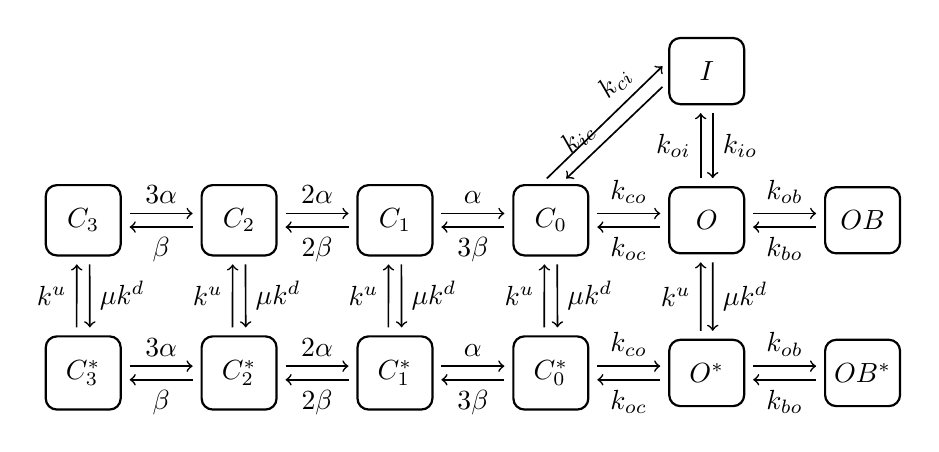
\begin{tikzpicture}[
   font=\sffamily,
   every matrix/.style={ampersand replacement=\&,column sep=1cm,row sep=1cm},
   state/.style={draw,thick,rounded corners,inner sep=.3cm},
   to/.style={->,semithick,shorten >=0.1cm,shorten <=0.1cm},
   Q/.style={->,semithick,sloped,pos=0.700000,shorten >=0.1cm,shorten <=0.1cm},  
   every node/.style={auto}]
\matrix{
\&\&\&\&\node[state] (I) {\parbox{10pt}{\centerline{$I$}}};\&\\
\node[state] (C_{3}) {\parbox{10pt}{\centerline{$C_{3}$}}};\&\node[state] (C_{2}) {\parbox{10pt}{\centerline{$C_{2}$}}};\&\node[state] (C_{1}) {\parbox{10pt}{\centerline{$C_{1}$}}};\&\node[state] (C_{0}) {\parbox{10pt}{\centerline{$C_{0}$}}};\&\node[state] (O) {\parbox{10pt}{\centerline{$O$}}};\&\node[state] (OB) {\parbox{10pt}{\centerline{$OB$}}};\\
\node[state] (C_{3}^{*}) {\parbox{10pt}{\centerline{$C_{3}^{*}$}}};\&\node[state] (C_{2}^{*}) {\parbox{10pt}{\centerline{$C_{2}^{*}$}}};\&\node[state] (C_{1}^{*}) {\parbox{10pt}{\centerline{$C_{1}^{*}$}}};\&\node[state] (C_{0}^{*}) {\parbox{10pt}{\centerline{$C_{0}^{*}$}}};\&\node[state] (O^{*}) {\parbox{10pt}{\centerline{$O^{*}$}}};\&\node[state] (OB^{*}) {\parbox{10pt}{\centerline{$OB^{*}$}}};\\
};
\draw[to]  (O^{*}.100) to node {$k^{u}$} (O.260);
\draw[to]  (O^{*}.10) to node {$k_{ob}$} (OB^{*}.170);
\draw[to]  (O^{*}.190) to node {$k_{oc}$} (C_{0}^{*}.350);
\draw[to]  (O.280) to node {$\mu k^{d}$} (O^{*}.80);
\draw[to]  (O.100) to node {$k_{oi}$} (I.260);
\draw[to]  (O.190) to node {$k_{oc}$} (C_{0}.350);
\draw[to]  (O.10) to node {$k_{ob}$} (OB.170);
\draw[to]  (I.280) to node {$k_{io}$} (O.80);
\draw[Q]  (I.195) to node {$k_{ic}$} (C_{0}.75);
\draw[to]  (C_{0}.10) to node {$k_{co}$} (O.170);
\draw[Q]  (C_{0}.105) to node {$k_{ci}$} (I.165);
\draw[to]  (C_{0}.190) to node {$3\beta$} (C_{1}.350);
\draw[to]  (C_{0}.280) to node {$\mu k^{d}$} (C_{0}^{*}.80);
\draw[to]  (C_{1}.10) to node {$\alpha$} (C_{0}.170);
\draw[to]  (C_{1}.190) to node {$2\beta$} (C_{2}.350);
\draw[to]  (C_{1}.280) to node {$\mu k^{d}$} (C_{1}^{*}.80);
\draw[to]  (C_{2}.10) to node {$2\alpha$} (C_{1}.170);
\draw[to]  (C_{2}.190) to node {$\beta$} (C_{3}.350);
\draw[to]  (C_{2}.280) to node {$\mu k^{d}$} (C_{2}^{*}.80);
\draw[to]  (C_{3}.10) to node {$3\alpha$} (C_{2}.170);
\draw[to]  (C_{3}.280) to node {$\mu k^{d}$} (C_{3}^{*}.80);
\draw[to]  (OB.190) to node {$k_{bo}$} (O.350);
\draw[to]  (OB^{*}.190) to node {$k_{bo}$} (O^{*}.350);
\draw[to]  (C_{0}^{*}.10) to node {$k_{co}$} (O^{*}.170);
\draw[to]  (C_{0}^{*}.100) to node {$k^{u}$} (C_{0}.260);
\draw[to]  (C_{0}^{*}.190) to node {$3\beta$} (C_{1}^{*}.350);
\draw[to]  (C_{1}^{*}.100) to node {$k^{u}$} (C_{1}.260);
\draw[to]  (C_{1}^{*}.10) to node {$\alpha$} (C_{0}^{*}.170);
\draw[to]  (C_{1}^{*}.190) to node {$2\beta$} (C_{2}^{*}.350);
\draw[to]  (C_{2}^{*}.100) to node {$k^{u}$} (C_{2}.260);
\draw[to]  (C_{2}^{*}.10) to node {$2\alpha$} (C_{1}^{*}.170);
\draw[to]  (C_{2}^{*}.190) to node {$\beta$} (C_{3}^{*}.350);
\draw[to]  (C_{3}^{*}.100) to node {$k^{u}$} (C_{3}.260);
\draw[to]  (C_{3}^{*}.10) to node {$3\alpha$} (C_{2}^{*}.170);
\end{tikzpicture}
\end{center}
\caption{This figure is a copy of Figure \ref{burstdrg} and it illustrates a Markov model of the mutant sodium channel.
 The model consists of the states $O,I,OB,C_{0}%
,C_{1},C_{2},$ and $C_{3}$ of the normal mode and $OB^*,O^{*},C^{*}_{0},C^{*}%
_{1},C^{*}_{2},$ and $C^{*}_{3}$ of the burst mode (lower part). }%
\label{wtreac3300}
\end{figure}

\subsubsection{Potassium current $I_{K}$}

The potassium current is written in the form
\begin{equation}
I_{K}= (o_{K} g_{K}(v) + g_{K1}(v)) (v-v_{K}),   \label{J_K}
\end{equation}
where the open probability $o_{K}$ is given by the Markov model of Figure  \ref{K1} with rates
\begin{align*}
\alpha(v) &  = e^{-7+0.03v},\\
\beta(v) &  = e^{-8-0.03v}. \\
\end{align*}
The voltage-dependent conductances are given by
\begin{align*}
g_K(v) &=  0.1 e^{-0.03v}, \\
g_{K1}(v) &= \frac{1}{1+e^{0.1 v+10}}. \\
\end{align*}


\begin{figure}[ptb]
\begin{center}
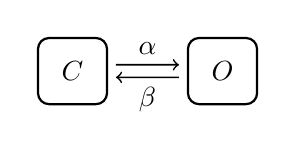
\begin{tikzpicture}[
   font=\sffamily,
   every matrix/.style={ampersand replacement=\&,column sep=1cm,row sep=1cm},
   state/.style={draw,thick,rounded corners,inner sep=.3cm},
   to/.style={->,semithick,shorten >=0.1cm,shorten <=0.1cm},
   Q/.style={->,semithick,sloped,pos=0.700000,shorten >=0.1cm,shorten <=0.1cm},
   every node/.style={auto}]
\matrix{
\node[state] (C) {$C$};\&\node[state] (O) {$O$};\\
};
\draw[to]  (O.190) to node {$\beta$} (C.350);
\draw[to]  (C.10) to node {$\alpha$} (O.170);
\end{tikzpicture}
\end{center}
\caption{Markov model of a potassium channel
consisting of one closed and one open state. }%
\label{K1}%
\end{figure}


\subsubsection{Calcium current $I_{Ca}$}

The calcium current is given by the calcium flux  $J_{d,e}$ from the dyad to the extracellular space plus the flux $J_{c,e}$ from the cytosol to the extracellular space.
In order to use these fluxes  in the equation governing the transmembrane potential, we need convert to current density,
\begin{equation}
I_{Ca}= 2 F\frac{V}{A} (-J_{d,e}-J_{c,e}).   \label{I_Ca}
\end{equation}
Here $V=30.4$ pL is the cell volume and $A=1.4\cdot 10^{-4} \text{ cm}^2$ is the cell area.

\subsection[Markov models as ODEs]{Markov models in terms of systems of differential equations}

The model of the action potential for a whole cell is a system of ordinary differential equations. For parts of the system this is clear from the equations,
but for the Markov models, this may seem unclear. In Section \ref{me_eq} we explained how to formulate a system of ordinary differential equation associated with the reaction scheme defining a Markov model.  Since the Markov models considered in the present chapter are considerably more complex, we will give one more example of this transition in order to clarify matters. To this end, consider the Markov model presented in Figure \ref{wtreac3331}. 
 The associated system of ordinary differential equations governing the probabilities is given by
\begin{align*}
o^{\prime}  & =k_{io}i+k_{co}c_{0}-\left(  k_{oc}+k_{oi}\right)  o,\\
i^{\prime}  & =k_{oi}o+k_{ci}c_{0}-\left(  k_{io}+k_{ic}\right)  i,\\
c_{0}^{\prime}  & =k_{oc}o+k_{ic}i+\alpha c_{1}-\left(  k_{co}+k_{ci}%
+3\beta\right)  c_{0},\\
c_{1}^{\prime}  & =3\beta c_{0}+2\alpha c_{2}-\left(  2\beta+\alpha\right)
c_{1},\\
c_{2}^{\prime}  & =2\beta c_{1}+3\alpha c_{3}-\left(  2\alpha+\beta\right)
c_{2},\\
c_{3}^{\prime}  & =\beta c_{2}-3\alpha c_{3}.%
\end{align*}
Here, $o$ denotes the open probability of the sodium channel,  $c_0$ is the probability of the $C_0$ state, and so forth. Ideally, we would write $o_{Na}$ for $o$, $c_{0,Na}$ for $c_0$, and so forth, but it becomes clumsy. Since these variables represent probabilities, they sum to one (for all time) and we can therefore reduce the number of unknowns in the system by one.

Based on this example, it should be straightforward to formulate the system of ordinary differential equations associated with the more complex Markov model given in Figure \ref{wtreac3300}.

\begin{figure}[ptb]
\begin{center}
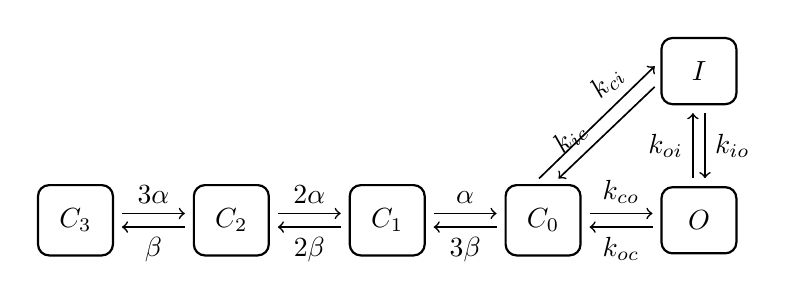
\begin{tikzpicture}[
   font=\sffamily,
   every matrix/.style={ampersand replacement=\&,column sep=1cm,row sep=1cm},
   state/.style={draw,thick,rounded corners,inner sep=.3cm},
   to/.style={->,semithick,shorten >=0.1cm,shorten <=0.1cm},
   Q/.style={->,semithick,sloped,pos=0.700000,shorten >=0.1cm,shorten <=0.1cm},  
   every node/.style={auto}]
\matrix{
\&\&\&\&\node[state] (I) {\parbox{10pt}{\centerline{$I$}}};\\
\node[state] (C_{3}) {\parbox{10pt}{\centerline{$C_{3}$}}};\&\node[state] (C_{2}) {\parbox{10pt}{\centerline{$C_{2}$}}};\&\node[state] (C_{1}) {\parbox{10pt}{\centerline{$C_{1}$}}};\&\node[state] (C_{0}) {\parbox{10pt}{\centerline{$C_{0}$}}};\&\node[state] (O) {\parbox{10pt}{\centerline{$O$}}};\\
};
\draw[to]  (O.100) to node {$k_{oi}$} (I.260);
\draw[to]  (O.190) to node {$k_{oc}$} (C_{0}.350);
\draw[to]  (I.280) to node {$k_{io}$} (O.80);
\draw[Q]  (I.195) to node {$k_{ic}$} (C_{0}.75);
\draw[to]  (C_{0}.10) to node {$k_{co}$} (O.170);
\draw[Q]  (C_{0}.105) to node {$k_{ci}$} (I.165);
\draw[to]  (C_{0}.190) to node {$3\beta$} (C_{1}.350);
\draw[to]  (C_{1}.10) to node {$\alpha$} (C_{0}.170);
\draw[to]  (C_{1}.190) to node {$2\beta$} (C_{2}.350);
\draw[to]  (C_{2}.10) to node {$2\alpha$} (C_{1}.170);
\draw[to]  (C_{2}.190) to node {$\beta$} (C_{3}.350);
\draw[to]  (C_{3}.10) to node {$3\alpha$} (C_{2}.170);
\end{tikzpicture}
\end{center}
\caption{Markov model of a wild type sodium channel consisting of an open
state $(O)$, an inactivated state $(I)$, and four closed states $(C_{0}%
,C_{1},C_{2}, \text{ and }C_{3})$. }%
\label{wtreac3331}%
\end{figure}


\section[Numerical action potential; wild type]{Numerical simulations using the action potential model for wild type Markov models}

The complete version of the model presented above can be written in the compact form
\begin{align}
Cv^{\prime}  & =-\left(  I_{Na}+I_{Ca}+I_{K}+I_{0}\right),  \label{s401}\\
u^{\prime}  & =F(v,u)\label{s402},%
\end{align}
where $v$ is the transmembrane potential and all other variables are gathered in the vector $u$. The initial conditions used in the simulations are given in Table \ref{tab:init}. In addition, we need to specify the applied current $I_0$. This current will be zero most of the time, but it will be turned on every 500 ms in order to mimic periodic stimulation of the cell. More specifically, 
we hold $I_0$ = -6 mV/ms for 5 ms at the start of each cycle.

\begin{table}
\begin{center}
\begin{tabular}{|c|c|} \hline
$v$ & -85 mV \\ \hline
$c_{d}$ & 0.1 $\mu$M \\ \hline
$c_{c}$ & 0.1 $\mu$M \\ \hline
$c_{j}$ & 1000 $\mu$M \\ \hline
$c_{n}$ & 1000 $\mu$M \\ \hline
$c_{e}$ & 1800 $\mu$M \\ \hline
\end{tabular} 
\caption{Initial conditions. The Markov models for the LCC and RyR were initially set to closed and the Markov model for sodium channel was set to be in the state $C_3$. Starting with these conditions, the code is run for 1000 cycles in order to generate the initial conditions used in generating the figures below. The exact numbers obtained depend upon the chosen cycle length. \label{tab:init}}
\end{center}
\end{table}





\subsection{Single action potential}

In Figure \ref{ap/single1.pdf} we show the transmembrane potential and all the calcium concentration for a single action potential. There are a number of interesting effects acting together to generate the action potential. Let us consider some of them in some detail. 

\fig[0.95]{ap/single1.pdf}{The action potential of the model described in the present chapter. The membrane potential (upper left) and the dynamics of the five
calcium concentrations are shown for 500 ms. The action potential is initiated by holding $I_0$ = -6 mV/ms for 5 ms. All variables return to their resting values after about 500 ms. }

\fig{ap/single2.pdf}{The first 20 ms of the simulation shown in Figure \ref{ap/single1.pdf}. Note the log scale in the upper right panel. There we see a slow rise due to the LCC opening, followed by a fast rise due to the RyR opening.}

In Figure \ref{ap/single2.pdf} we show the first 20 ms of the computation. In the left panel we show the transmembrane potential $v$ (upper left panel), the open probability $o_{Na}$ (middle left panel), and the sodium current $I_{Na}$ (lower left panel). Observe that when the cell is stimulated by the applied current $I_0$, the transmembrane potential increases. This increase leads to an increased open probability of the sodium channel. When the sodium channel opens, the sodium current becomes large (or very negative, to be precise), which leads to a fast increase of the transmembrane potential. As the transmembrane potential reaches its peak value (at about 15 ms), the open probability starts to decline, since the channel inactivates. In the three right panels, we show the calcium concentration of the dyad $c_d$ (upper right panel), the calcium flux $J_{d,e}$ (middle right panel), and the open probability of the RyR channel  (lower right panel). We see that when the transmembrane potential starts increasing, the calcium flux $J_{d,e}$ increases and the calcium concentration of the dyad increases. This increase leads to the increased open probability (lower right panel) of the RyR channel and therefore the dyad concentration increases rapidly. 

In Figure \ref{ap/single3.pdf}, we show the return to the stable equilibrium solution. In the left panel, we show the transmembrane (upper left panel), the open probability of the LCC (middle left panel), and the open probability of the gated potassium channel. After the sodium channel has switched off (see Figure \ref{ap/single2.pdf}), the calcium current contributes to a continued depolarized state. However, after about 20 ms the transmembrane potential starts declining because of a substantial (positive) potassium current. 
%the open probability $o_{Na}$ (middle left panel), and the potassium current $I_K$ (lower left panel). We see that the sodium channel now is not conducting since $o_{Na}$ is almost zero. The transmembrane potential is reduced and this is due to a substantial (positive) potassium current. 

In the right panels, we follow the development of the calcium concentration of the dyad $c_d$ (upper right panel),  the calcium concentration 
\GTLV{$c_j$ of the JSR},
%$c_n$ of the NSR 
(middle right panel), and the open probability of the RyR channel, denoted $o_{j,d}$ (lower right panel). 
%\GTLV{we see that the jSR consentration falls rapidly when channel is open. This causes the channel to close, due an incrase in the half-maximum  constant (see 
%$equation \ref{halfmax})}.
%We see that the dyad concentration is reduced and that the RyR is practically closed. The increase of the calcium concentration in the NSR is due to the pump $J_{c,n}$ and to the fact that the RyR channel is closed. 

\fig{ap/single3.pdf}{After about 15 ms, the transmembrane potential (upper left) reaches its peak value and enters the plateau phase before it starts to decline toward the stable equilibrium solution. }


\subsection{Many action potentials}

In Figure \ref{ap/multiple.pdf}, we show the action potential for a simulation running for 25,000 ms. The left panel shows the transmembrane potential $v$ (upper left panel), the calcium concentration $c_d$ of the dyad (middle left panel), and the extracellular calcium concentration $c_e$ (lower left panel). From top to bottom in the right panels, we show the cytosolic calcium concentration $c_c$, the NSR calcium concentration $c_n$, and finally the JSR calcium concentration $c_j$. All variables return to their initial values and the rhythm seems to be perfect. 
%In Figure xxx5, we show exactly the same variables after 10000 action potentials and it looks exactly the same. 

\fig{ap/multiple.pdf}{The action potential running for 25,000 ms (50 beats). All variables return to their equilibrium values before a new action potential is initiated (every 500 ms). }

\section[Changing the mean open time]{Changing the mean open time of the sodium channel while keeping the equilibrium probability fixed changes the action potential \label{sec:ap_mot}}

We consider a case where we multiply all rates of the Markov model (see Figure \ref{wtreac3300}) of the sodium channel by the same factor. Here we use the wild type case ($\mu=1$) and the drug parameters ($k_{ob}, k_{bo}$) are set to zero. This will change the mean open time, but not the equilibrium probabilities. The results are given in Figure \ref{ap/mot.pdf}, where the blue line illustrates the results using default parameters, the red line represents the solution when all the rates are multiplied by 1.3, and finally the green line represents the solution when all the rates are multiplied by 0.7. We observe that the action potential changes substantially when the rates are changed (and the mean open time is changed), even though the equilibrium probabilities are kept unchanged.

\fig{ap/mot.pdf}{Slower dynamics (green) lead to later inactivation, yielding a higher plateau. Quicker dynamics (red) lead to faster recovery from inactivation, allowing a stronger late current. }




\section[Numerical action potential; mutations]{Numerical simulations using the action potential model when the cell is affected by a mutation}

We will use the model of the action potential for the whole cell introduced above to study the effect of mutations. We have studied many different theoretical models of mutations earlier, but here we will limit ourselves to study the effect of one theoretical model of a sodium channel mutation, one model of a RyR mutation, and one model of an LCC mutation. We will also see how the theoretical drugs derived above handle these mutations.




\subsection{Mutation of the sodium channel}

We consider a mutation of the sodium channel of the form presented in Figure \ref{wtreac3300}. 
In Figure \ref{ap/burst_mut.pdf} we show simulation results comparing the wild type ($\mu=1$, blue),
the mutant ($\mu=10$, green), and a simulation (red) where  a drug is applied to the mutant case.
The Markov model describing the open state drug is given
in Figure \ref{wtreac3300}, where we have used drug parameters given by
\[
k_{bo} = k_{io}, \mbox{\ and \ }
k_{ob}=\left(  \mu-1\right)  \frac{k^{d}k^{u}k_{oi}}{\left(  k^{u}+\mu
k^{d}\right)  \left(  k^{u}+k^{d}\right)  };%
\]
see (\ref{na_drug_ob}) and (\ref{na_drug_bo}).
As in the single channel case, we observe that the theoretical drug is able to repair the effect of the mutation. 






\fig{ap/burst_mut.pdf}{The figure shows the action potential of the wild type (blue), the mutant (green), and the
mutant after the application of the drug (red).}


\subsection{Mutation of the RyR}

In Figure \ref{ap/ryr_mut.pdf} we have simulated mutation in the RyR using the Markov model given in Figure \ref{eq:m_rl2}. The figure shows the
wild type (blue, $\mu=1$), the mutant (green, $\mu=3$), and the mutant where the drug has been applied (red). We have used a closed state drug  computed as described in (\ref{closed_drg}) and (\ref{optimal_closed_charac}) and we observe that the theoretical drug is able to repair the effect of the mutation. 
%{\bf xxxGTL: Is this a RyR mutation?  If RYR- what is the Markov model with drugs? Refs to model}

%\GTL{Mutation model and drug as defined in (\ref{closed_drg}) and (\ref{optimal_closed_charac}). As usual $k_{bc}$ is a free parameter that should be large enough.}

%\GTL{If we want a new figure we could expand Figure 15.2 to a 2x3 matrix here, and then to a 3x2 matrix in the next section. Or make a 3x3 figure from the start. In reality LCC and RyR are implemented as stand-alone models, so we could also have 1x3 matrix, here and below, like in (\ref{closed_drg}), or just refer to this figure. Perhaps best to split Figure 15.2 into an RyR and and LCC figure.}


\fig{ap/ryr_mut.pdf}{The cytosolic calcium concentration for wild type (blue, $\mu=1$), the mutant (green, $\mu=3$), and the mutant after the application of the drug (red). 
We have used a closed state drug  as defined in (\ref{closed_drg}) with $k_{bc}=0.5$ ms$^{-1}$ and $k_{cb}=(\mu-1)k_{bc}$; see (\ref{optimal_closed_charac}). }

\subsection{Mutation of the LCC}

In Figure \ref{ap/lcc_mut.pdf} we have simulated mutation in the LCC channel, using $\eta=3$. 
%{\bf xxxGTL: Is this a LCC mutation?  If LCC- what is the Markov model with drugs? Refs to model}
We model the mutation and the drug as defined in (\ref{closed_drg}) and (\ref{optimal_closed_charac}). As usual, $k_{bc}$ is a free parameter that must be chosen sufficiently large. Again, we note that the theoretical drug repairs the effect of the mutation. 

\fig{ap/lcc_mut.pdf}{LCC mutation. The cytosolic calcium concentration for the wild type (blue, $\eta=1$), the mutant (green $\eta=3$), and the mutant case where the theoretical drug is applied (red). In the computations we have used $k_{bc}=0.05$ ms$^{-1}$; for larger values of $k_{bc}$ the results overlap with the
wild type case.}


\clearpage
\section{Notes}
\begin{enumerate}
\item The action potential model discussed in Section \ref{sec:ap} and used throughout this chapter is only of qualitative relevance; no effort is made to mimic the properties of one particular cell. The field of models for the action potential is huge and growing. A great collection of models is provided by the Auckland Bioengineering Institute at the University of Auckland and their collaborators; see CellML.org. Recent models tend to be increasingly complex and hard to deal with from a mathematical perspective, but clearly the models become more and more realistic in terms of mimicking the properties of the actual action potential.  As mentioned earlier, there are comprehensive introductions to the cardiac action potential, such as Rudy \cite{Rudy2012} and Rudy and Silva \cite{Rudy2006}.
\item In these notes we have used Matlab as the computational platform for all our simulations. For solving ordinary differential equations we have used the ODE15s function. However, solving the ordinary differential equations modeling the single cell action potential has received a great deal of attention and numerical methods suited for this problem have been developed. An early alternative was developed by Rush and Larsen \cite{Rush1978}; the method was improved to second by Sundnes et al.  \cite{Sundnes2009} and comparisons of several methods were provided by Marsh et al. \cite{Marsh2012} and Campos et al. \cite{Campos2013}; see also Stary and Biktashev \cite{Stary2015}. From a programming perspective, the explicit Euler scheme is always an attractive alternative, but for stiff problems the stability requirement often excludes that method. For instance, if we use the explicit Euler method with a fixed time step to compute the solutions shown in  Figure \ref{ap/single1.pdf}, we need about 26000 time-steps, whereas the ODE15s method needs 335 time steps.

\end{enumerate}

%\input{Potassium_L/blocker}
%\input{Potassium_L/K}


%\bibliographystyle{unsrt}
\bibliographystyle{plain}
\bibliography{ln}
\end{document}
